\documentclass[thmcnt=section, 12pt]{my-elegantbook}

% index page
\usepackage{imakeidx}
\makeindex[columns=2, intoc, options=-s index_style.ist]

% title and author
\title{Mathematical Analysis}
\author{Isaac FEI}

% reference file
\addbibresource{Mathematical Analysis.bib} 

% image of the book cover
\cover{cover}

\begin{document}

% Print title and cover page
\maketitle

%--------
% preface
%--------

\frontmatter
\section*{Preface}

This book mainly follows the structure of \parencite{apostolMathematicalAnalysisModern1974}.

%------------------------------

% Print table of contents
\tableofcontents
\mainmatter

%-------------------------------
% main document starts from here
%-------------------------------

%==============================

\chapter{Set Theory}

%------------------------------

\section{Properties of Suprema and Infima}

\begin{theorem} \label{thm:27}
    Let $f: X \to \R$ be a real-valued function. We have the following equation.
    \begin{align}
        \sup_{x \in X} f(x) - \inf_{x \in X} f(x)
        = \sup_{x,y \in X} [f(x) - f(y)]
        \label{eq:66}
    \end{align}
\end{theorem}

\begin{proof}
    Let $M$ and $m$ denote 
    \begin{align*}
        M = \sup_{x \in X} f(x)
        \quad\text{and}\quad
        m = \inf_{x \in X} f(x)
    \end{align*}
    We have 
    \begin{align*}
        f(x) - f(y) \leq M - m
        \quad \forall x,y \in X
    \end{align*}
    It then follows that 
    \begin{align}
        \sup_{x,y \in X} [f(x) - f(y)]
        \leq M - m
        \label{eq:67}
    \end{align}

    On the other hand, given $\varepsilon > 0$, there exists $x, y \in X$ such that 
    \begin{align}
        f(x) > M - \varepsilon / 2
        \quad \text{and} \quad 
        f(y) < m + \varepsilon / 2
    \end{align} 
    It follows that 
    \begin{align*}
        \sup_{x,y \in X} [f(x) - f(y)]
        \geq f(x) - f(y)
        > M - m - \varepsilon
    \end{align*}
    Because 
    \begin{align*}
        \sup_{x,y \in X} [f(x) - f(y)]
        > M - m - \varepsilon
    \end{align*}
    holds for any $\varepsilon > 0$, we have 
    \begin{align}
        \sup_{x,y \in X} [f(x) - f(y)]
        \geq M - m
        \label{eq:68}
    \end{align}
    Then, equation \eqref{eq:66} follows from \eqref{eq:67} and \eqref{eq:68}.
\end{proof}

%==============================

\chapter{Numerical Sequences and Series}

We are interested in real or complex-valued sequences and series.

%------------------------------

\section{Monotonic Sequences of Real Numbers}

\begin{theorem} \label{thm:57}
    A monotonic sequence $\{a_n\}$ converges if and only if it is bounded. Furthermore, assuming $\{a_n\}$ does converge, 
    \begin{enumerate}
        \item $\lim_{n \to \infty} a_n = \sup_{n \in \N^\ast} a_n$ if $\{a_n\}$ is increasing, and
        \item $\lim_{n \to \infty} a_n = \inf_{n \in \N^\ast} a_n$ if $\{a_n\}$ is decreasing.
    \end{enumerate}
\end{theorem}

%------------------------------

\section{Limit Superior and Limit Inferior}

Given a real-valued sequence $\{a_n\}$, sometimes the information about the upper and lower bounds of the \textit{entire} sequence, if they exist, may not be useful for we are often interested in the \textbf{tail}\index{tail of a sequence} of the sequence, which is simply the portion of $\{a_n\}$ after a few indices. To be  specific, the $n$-th tail of $\{a_n\}$ is defined by $\{a_{m+n-1}\}_{m \in \N^\ast}$, and is written as $\{a_m\}_{m \geq n}$ in shorthand.

If $\{a_n\}$ is bounded, we can define two sequences of upper and lower bounds, $\{u_n\}$ and $\{l_n\}$, of the tail $\{a_m\}_{m \geq n}$ by
\begin{align*}
    u_n = \sup_{m \geq n} a_m
    \quad \text{and} \quad
    l_n = \inf_{m \geq n} a_m,
    \quad n \in \N^\ast
\end{align*}
To study the limiting behavior of $\{a_n\}$, it is helpful to know how the $n$-th tail $\{a_m\}_{m \geq n}$ is bounded when $n$ is relatively large.

At a first glance, we observe that $\{u_n\}$ is decreasing and $\{l_n\}$ is increasing, which we shall prove in the next lemma.

\begin{lemma} \label{lem:5}
    Let $\{a_n\}$ be a sequence of real numbers.
    \begin{enumerate}
        \item If $\{a_n\}$ is bounded above, for each integer $n \in \N^\ast$ we can define
        \begin{align*}
            u_n = \sup_{m \geq n} a_m,
            \quad n \in \N^\ast
        \end{align*}
        The sequence $\{u_n\}$ is decreasing.
        \item If $\{a_n\}$ is bounded below, for each integer $n \in \N^\ast$ we can define
        \begin{align*}
            l_n = \inf_{m \geq n} a_m,
            \quad n \in \N^\ast
        \end{align*}
        The sequence $\{l_n\}$ is increasing.
    \end{enumerate}
\end{lemma}

\begin{proof}
    We only prove 1. For every $m \in \N^\ast$ with $m \geq n+1$, it is clear
    \begin{align*}
        a_{m} \in \set{a_m}{m \geq n, n \in \N^\ast}
    \end{align*}
    Note that $u_n$ is an upper bound of the set on the right-hand side. Hence, 
    \begin{align*}
        a_m \leq u_n
        \quad \forall m \geq n+1
    \end{align*}
    This implies $u_n$ is also an upper bound of 
    \begin{align*}
        \set{a_m}{m \geq n+1, n \in \N^\ast}
    \end{align*}
    It then follows that $u_{n+1} \leq u_n$ since $u_{n+1}$ is the least upper bound of the set above. Therefore, we have shown 
    \begin{align*}
        u_{n} \geq u_{n+1}
        \quad \forall n \in \N^\ast
    \end{align*}
    Hence, $\{u_n\}$ is decreasing.
\end{proof}

%------------------------------

\subsection{Definition}

By Theorem~\ref{thm:57}, we know that the limits of $\{u_n\}$ and $\{l_n\}$ always exist (as finite or infinite numbers). This gives rise to the definitions of limit superior as well as limit inferior. We also take into consideration the cases where $\{a_n\}$ is not bounded.

\begin{definition}
    Let $\{a_n\}$ be a sequence of real numbers. The \textbf{limit superior}\index{limit superior} of $\{a_n\}$, denoted by $\limsup_{n \to \infty} a_n$, is defined as follows:
    \begin{enumerate}
        \item $\limsup_{n \to \infty} a_n := \infty$ if $\{a_n\}$ is not bounded above, and 
        \item $\limsup_{n \to \infty} a_n := \lim_{n \to \infty} u_n$ if $\{a_n\}$ is bounded above where $u_n = \sup_{m \geq n} a_m$.
    \end{enumerate}
    The \textbf{limit inferior}\index{limit inferior} of $\{a_n\}$ is denoted by $\liminf_{n \to \infty} a_n$ and is defined similarly.
\end{definition}

\begin{note}
    The notation $\limsup$ consists of two parts, the limit symbol and the supremum symbol. Indeed, as we can see from the definition, this notation arises naturally for we can write
    \begin{align*}
        \limsup_{n \to \infty} a_n
        = \lim_{n \to \infty} \sup_{m \geq n} a_m
    \end{align*}
    if $\{a_n\}$ is bounded above.
\end{note}

\begin{example}
    Let
    \begin{align*}
        a_n = \brk{1 + \frac{10}{n}} \sin \frac{n \pi}{32}
    \end{align*}
    We claim that the limit superior and limit inferior of $\{a_n\}$ are $1$ and $-1$, respectively. See Figure~\ref{fig:12}.

    \begin{figure}[ht]
        \centering
        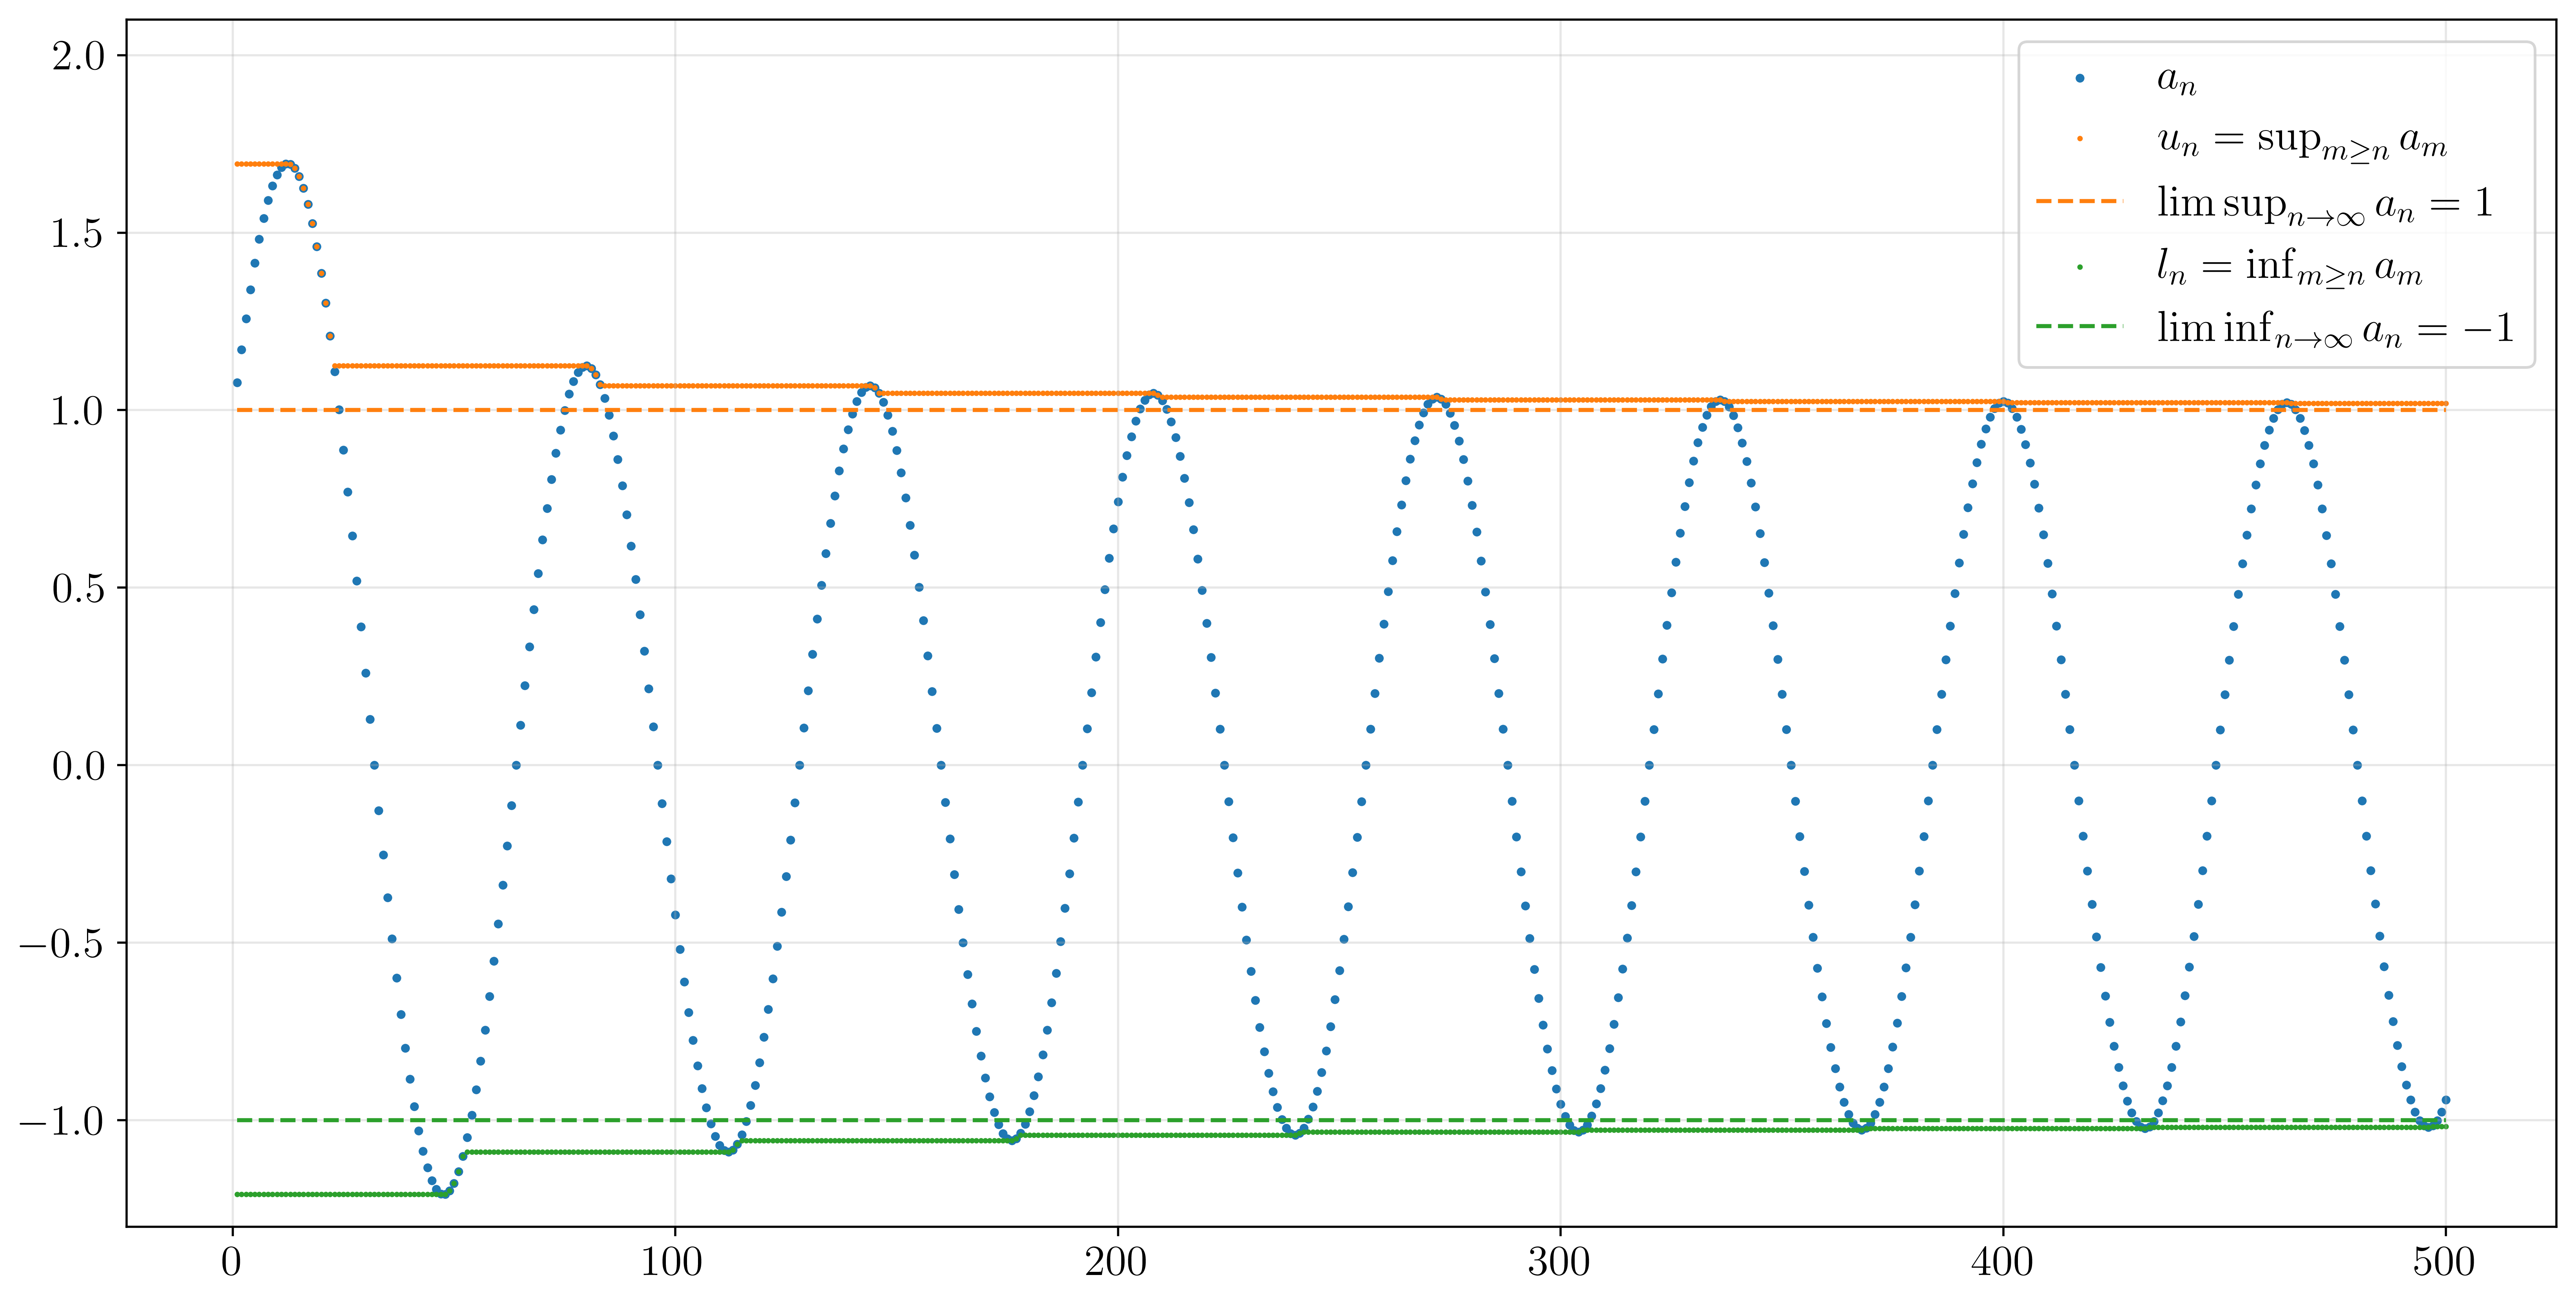
\includegraphics[scale=0.4]{figures/limsup-liminf.png}
        \caption{Limit superior and limit inferior of $\{a_n\}$ where $a_n = \brk{1 + \frac{10}{n}} \sin \frac{n \pi}{32}$.}
        \label{fig:12}
    \end{figure}

    Now, we show that the values of limit superior and limit inferior are indeed as claimed. Note that for any given integer $n \in \N^\ast$, we can choose an integer $k$ such that $16 + 64k \geq n$. Let $m = 16 + 64k$. We have 
    \begin{align*}
        a_m = \brk{1 + \frac{10}{m}} \sin \frac{(16 + 64k) \pi}{32}
        = \brk{1 + \frac{10}{m}} \sin \brk{
            \frac{\pi}{2} + 2k\pi
        }
        = 1 + \frac{10}{m}
        > 1
    \end{align*}
    This implies that 
    \begin{align}
        u_n = \sup_{m \geq n} a_m > 1
        \quad \forall n \in \N^\ast
    \end{align}
    which means the sequence $\{u_n\}$ is bounded below by $1$. We know by Lemma~\ref{lem:5} that $\{u_n\}$ is decreasing. Thus, by Theorem~\ref{thm:57}, $\{u_n\}$ converges to the infimum of its range, $\inf_{n \in \N^\ast} u_n$. We need to show that $\inf_{n \in \N^\ast} u_n = 1$. Given $\varepsilon > 0$, there exists $n \in \N^\ast$ such that $10 / n < \varepsilon/2$. Then, for every $m \geq n$, we have 
    \begin{align*}
        1 + \frac{10}{m} < 1 + \varepsilon/2
    \end{align*}
    Because the absolute value of the sine function is bounded by $1$, it follows that 
    \begin{align*}
        a_m = \brk{1 + \frac{10}{m}} \sin \frac{m \pi}{32} < 1 + \varepsilon/2
        \quad \forall m \geq n
    \end{align*}
    Taking the supremum, we obtain
    \begin{align*}
        u_n = \sup_{m \geq n} a_m
        \leq 1 + \varepsilon/2
        < 1 + \varepsilon
    \end{align*}
    Therefore, 
    \begin{align*}
        \limsup_{n \to \infty} a_n
        = \lim_{n \to \infty} u_n
        = \inf_{n \in \N^\ast} u_n = 1
    \end{align*}
    The proof of $\liminf a_n = -1$ is similar and is left as an exercise.
\end{example}

%------------------------------

When the limit superior/inferior of $\{a_n\}$ is finite, then we have the following equivalent conditions, which may be helpful in proofs.

\begin{theorem} \label{thm:58}
    Let $\{a_n\}$ be a sequence of real numbers. Suppose there exists a (finite) number $u$ satisfying the following two conditions:
    \begin{enumerate}
        \item For every $\varepsilon > 0$, there exists an integer $N$ such that 
        \begin{align*}
            a_n < u + \varepsilon
            \quad \forall n \geq N
        \end{align*}
        \item Given $\varepsilon > 0$ and given an integer $m$, there exists an integer $N \geq m$ such that 
        \begin{align*}
            a_N > u - \varepsilon
        \end{align*}
    \end{enumerate}
    Then $u$ is the limit superior of $\{a_n\}$, i.e., $u = \limsup a_n$. Conversely, if $u = \limsup a_n$ is a finite number, then it satisfies the above conditions. An analogous result exists concerning the limit inferior of $\{a_n\}$.
\end{theorem}

Given $\varepsilon > 0$, the first condition says $u+\varepsilon$ is an upper bound for some $N$-th tail of $\{a_n\}$. In other words, all the terms of $\{a_n\}$ will eventually fall below the number $u + \varepsilon$. While the second condition says there are \textit{infinitely} many terms of $\{a_n\}$ that exceed $u - \varepsilon$.

\begin{note}
    These two conditions are used to define the limit superior in Apostol's book\cite{apostolMathematicalAnalysisModern1974}. The problem is that we cannot assume the existence of such a number $u$ if we adopt this definition, although the existence can be proved later. But this would increase the difficulty in understanding the concept of limit superior/inferior. 
\end{note}

\begin{proof}
    (Sufficiency) We first assume $u$ satisfies the above two conditions and show that it is indeed the limit superior of $\{a_n\}$. Note that the first condition implies that $\{a_n\}$ is bounded above. Hence, it is feasible to define 
    \begin{align*}
        u_n = \sup_{m \geq n} a_m,
        \quad n \in \N^\ast
    \end{align*}
    By Lemma~\ref{lem:5}, we know $\{u_n\}$ is decreasing. Let $m \in \N^\ast$ be fixed for now, by exploiting the second condition, for any $\varepsilon > 0$, there exists an integer $N \geq m$ such that 
    \begin{align*}
        a_N > u - \varepsilon
    \end{align*}
    It then follows that 
    \begin{align*}
        u_m = \sup_{n \geq m} a_n
        \geq a_N
        > u - \varepsilon
    \end{align*}
    Since 
    \begin{align*}
        u_m > u - \varepsilon
    \end{align*}
    holds for any $\varepsilon > 0$. We have 
    \begin{align}
        u_m \geq u
        \label{eq:118}
    \end{align}
    But $m \in \N^\ast$ is also chosen arbitrarily. Therefore, the above inequality implies that the sequence $\{u_n\}$ is bounded below by $u$.

    Next, we show that $u$ is the infimum of the range of $\{u_n\}$. Given $\varepsilon > 0$, by condition 1, there exists $N \in \N^\ast$ such that 
    \begin{align*}
        a_n < u + \varepsilon/2
        \quad \forall n \geq N
    \end{align*}
    Taking the supremum over $n$, we obtain 
    \begin{align*}
        u_N = \sup_{n \geq N} a_n 
        \leq u + \varepsilon/2
        < u + \varepsilon
    \end{align*}
    That is, 
    \begin{align}
        u_N < u + \varepsilon
        \label{eq:119}
    \end{align}

    It then follows from \eqref{eq:118} and \eqref{eq:119} that
    \begin{align*}
        u = \inf_{n \in \N^\ast} u_n
    \end{align*} 
    Recall $\{u_n\}$ is decreasing. Then by Theorem~\ref{thm:57}, $\lim u_n$ is precisely the infimum of its range since it is bounded below. Finally, since the limit superior of $\{a_n\}$ is defined by $\lim u_n$, we conclude that $u = \limsup a_n$.

    (Necessity) Assume that the limit superior of $\{a_n\}$, $u$, is a finite number. By definition, $\{a_n\}$ is bounded above. Hence, we can again define 
    \begin{align*}
        u_n = \sup_{m \geq n} a_m,
        \quad n \in \N^\ast
    \end{align*}
    And by definition along with the fact that $\{u_n\}$ is decreasing, we have 
    \begin{align*}
        u = \lim_{n \to \infty} u_n
        = \inf_{n \in \N^\ast} u_n
    \end{align*}
    We need to show $u$ indeed satisfies the two conditions stated in this theorem.

    Given $\varepsilon > 0$, since $u = \inf u_n$, there exists $N \in \N^\ast$ such that 
    \begin{align*}
        u_N < u + \varepsilon
    \end{align*}
    But $u_N = \sup_{n \geq N} a_n$. Therefore, 
    \begin{align*}
        \sup_{n \geq N} a_n < u + \varepsilon
    \end{align*}
    And because $a_n \leq \sup_{n \geq N} a_n \; \forall \geq N$, we have 
    \begin{align*}
        a_n < u + \varepsilon
        \quad \forall n \geq N
    \end{align*}
    This shows that $u$ satisfies condition 1.

    Given $\varepsilon > 0$ and $m \in \N^\ast$. Because $u$ is a lower bound of $\{u_n\}$, we have 
    \begin{align}
        \sup_{n \geq m} a_n = u_m \geq u
        \label{eq:120}
    \end{align}
    By the property of supremum, there exists an integer $N \geq m$ such that 
    \begin{align}
        a_N > \sup_{n \geq m} a_n - \varepsilon
        \label{eq:121}
    \end{align}
    Combining \eqref{eq:120} with \eqref{eq:121}, we find
    \begin{align*}
        a_N > u - \varepsilon
    \end{align*}
    which implies that $u$ also satisfies condition 2. This completes the proof.
\end{proof}

%------------------------------

\subsection{Properties}

\begin{proposition} \label{pro:6}
    Let $\{a_n\}$ be a sequence of real numbers. Then 
    \begin{enumerate}
        \item $\limsup a_n = -\infty \implies \liminf a_n = -\infty$, and
        \item $\{a_n\}$ diverges to $-\infty$ if and only if $\limsup a_n = \liminf a_n = -\infty$.
    \end{enumerate}
\end{proposition}

\begin{proof}
    (Proof of 1) Note that the fact that the limit superior is not positive infinity implicitly implies that $\{a_n\}$ is bounded above. Define 
    \begin{align}
        u_n = \sup_{m \geq n} a_m,
        \quad n \in \N^\ast
        \label{eq:122}
    \end{align}
    We have $\lim u_n = -\infty$. Hence, for every $M > 0$, there exists $N \in \N^\ast$ such that 
    \begin{align*}
        u_n \leq -M
        \quad \forall n \geq N
    \end{align*}
    But $a_n \leq \sup_{m \geq n} a_m = u_n$. It follows that 
    \begin{align*}
        a_n \leq -M
        \quad \forall n \geq N
    \end{align*}
    This implies $\{a_n\}$ diverges to $-\infty$, that is, $\lim a_n = -\infty$. As a consequence, $\{a_n\}$ is not bounded below. Therefore, $\liminf a_n = -\infty$ by definition.

    (Proof of 2) Note that in proving the first statement, we have already shown that $\limsup a_n = \liminf a_n = -\infty$ implies $\lim a_n = -\infty$. We only need to prove the other direction. Suppose $\lim a_n = -\infty$. For every $M > 0$, there exists $N \in \N^\ast$ such that 
    \begin{align*}
        a_n \leq -M
        \quad \forall n \geq N
    \end{align*}
    \begin{note}
        Note that the above inequality implies that $\{a_n\}$ is bounded above. Hence, we can again define $\{u_n\}$ as in \eqref{eq:122}.
    \end{note}
    \noindent Taking the supremum over $n$, we obtain
    \begin{align*}
        u_N = \sup_{n \geq N} a_n \leq -M
    \end{align*}
    Note that $\{u_n\}$ is decreasing by Lemma~\ref{lem:5}. Hence,
    \begin{align*}
        u_n \leq u_N \leq -M
        \quad \forall n \geq N
    \end{align*}
    This implies that $\lim u_n = -\infty$. Therefore, by the definition of limit superior, $\limsup a_n = -\infty$. Then by statement 1, which we have proved earlier, $\liminf a_n = -\infty$.
\end{proof}

As an analogous result, we also have the following proposition, the proof of which is similar and is left as an exercise.

\begin{proposition} \label{pro:4}
    Let $\{a_n\}$ be a sequence of real numbers. Then 
    \begin{enumerate}
        \item $\liminf a_n = \infty \implies \limsup a_n = \infty$, and
        \item $\{a_n\}$ diverges to $\infty$ if and only if $\limsup a_n = \liminf a_n = \infty$.
    \end{enumerate}
\end{proposition}

%------------------------------

\begin{proposition} \label{pro:5}
    Let $\{a_n\}$ be a sequence of real numbers. Then $\{a_n\}$ converges if and only if both limit superior and limit inferior are equal to a finite number. That is, 
    \begin{align*}
        \lim a_n = a
        \iff
        \limsup a_n = \liminf a_n = a
    \end{align*}
    where $a$ is finite.
\end{proposition}

\begin{proof}
    (Sufficiency) Suppose that the limit superior and limit inferior are equal to a finite number, i.e.,  $\limsup a_n = \liminf a_n = a$. Let $\varepsilon > 0$ be chosen arbitrarily. Because $a$ is the limit superior, by the first condition in Theorem~\ref{thm:58}, there exists $N_1 \in \N^\ast$ such that 
    \begin{align*}
        a_n < a + \varepsilon
        \quad \forall n \geq N_1
    \end{align*}
    Similarly, if we treat $a$ as the limit superior, then there exists $N_2 \in \N^\ast$ such that 
    \begin{align}
        a_n > a - \varepsilon
        \quad \forall n \geq N_2
    \end{align}
    Let $N = \max\{N_1, N_2\}$. We have 
    \begin{align*}
        \abs{a_n - a} < \varepsilon
        \quad \forall n \geq N
    \end{align*}
    Therefore, $\{a_n\}$ converges to $a$.

    (Necessity) Suppose $\{a_n\}$ converges to $a$. Given $\varepsilon > 0$, there exists $N \in \N^\ast$ such that 
    \begin{align*}
        \abs{a_n - a} < \varepsilon
        \quad \forall n \geq N
    \end{align*}
    We have 
    \begin{enumerate}
        \item $a_n < a + \varepsilon$ for all $n \geq N$, and 
        \item for any given $m \in \N^\ast$, there exists $M \geq \max\{m, N\}$ such that $a_M > a - \varepsilon$.
    \end{enumerate}
    By Theorem~\ref{thm:58}, $a = \limsup a_n$. Similarly, we can also show $a = \liminf a_n$.
\end{proof}

%------------------------------

Like the limit and supremum/infimum, limit superior/inferior also preserves the order.

\begin{theorem} \label{thm:59}
    If $a_n \leq b_n \; \forall n \in \N^\ast$, then 
    \begin{align*}
        \limsup a_n \leq \limsup b_n 
        \quad \text{and} \quad 
        \liminf a_n \leq \liminf b_n 
    \end{align*}
\end{theorem}

\begin{proof}
    We only prove $\limsup a_n \leq \limsup b_n$. 

    (Extreme Cases) If $\limsup a_n = -\infty$ or $\limsup b_n = \infty$, then there is nothing to prove. If $\limsup a_n = \infty$, then $\{a_n\}$ is not bounded above and nor is $\{b_n\}$, and hence $\limsup b_n = \infty$. Suppose $\limsup b_n = -\infty$, then $\lim b_n = -\infty$ by Proposition~\ref{pro:6}. It follows that $\lim a_n = -\infty$, and hence $\limsup a_n = -\infty$.

    (Finite Limit Superiors) Now, suppose that $\limsup a_n$ and $\limsup b_n$ are both finite. We have 
    \begin{align*}
        \sup_{m \geq n} a_m \leq \sup_{m \geq n} b_m
        \quad \forall n \in \N^\ast
    \end{align*}
    Taking the limit on both sides yields
    \begin{align*}
        \limsup a_n
        = \lim_{n \to \infty} \sup_{m \geq n} a_m 
        \leq \lim_{n \to \infty} \sup_{m \geq n} b_m
        = \limsup b_n
    \end{align*}
\end{proof}

%------------------------------

The next theorem can be treated as the reciprocal rule of limit superior, which establishes the relation between $\limsup 1 / a_n$ and $\liminf a_n$.

\begin{theorem} \label{thm:60}
    Let $\{a_n\}$ be a sequence of positive numbers, then 
    \begin{enumerate}
        \item $\limsup \frac{1}{a_n} = 1 / \liminf a_n$, and 
        \item $\liminf \frac{1}{a_n} = 1 / \limsup a_n$.
    \end{enumerate}
    Note that, in the first equation, if $\liminf a_n = 0$ then $\limsup 1 / a_n = \infty$, and $\limsup 1 / a_n = 0$ if $\liminf a_n = \infty$. A similar treatment also applies to the second equation.
\end{theorem}

\begin{proof}
    We only prove 1 since the second equation can be obtained by replacing $a_n$ with $1 / a_n$ in the first one. 

    (Case 1: $\liminf a_n = 0$.) For every positive number $M > 0$. By Theorem~\ref{thm:58} (the second condition for limit inferior), there exists $N \in \N^\ast$ such that 
    \begin{align*}
        a_N < 0 + \frac{1}{M} = \frac{1}{M}
    \end{align*}
    Taking the reciprocal, we find
    \begin{align*}
        \frac{1}{a_N} > M
    \end{align*}
    This implies that the sequence $\{1 / a_n\}$ is not bounded above. Hence, $\limsup 1 / a_n = \infty$ by definition.

    (Case 2: $\liminf a_n = \infty$.) We know $\lim a_n = \infty$ by Proposition~\ref{pro:4}. This implies $\{1 / a_n\}$ will converge to zero, i.e., $\lim 1 / a_n = 0$. By Proposition~\ref{pro:5}, $\limsup a_n = 0$.

    (Case 3: $\liminf a_n$ is a finite positive number.) Write $l = \liminf a_n$. Let $\varepsilon > 0$ be chosen arbitrarily. Put 
    \begin{align*}
        \varepsilon_1 = \frac{\varepsilon l^2}{1 + \varepsilon l}
    \end{align*}
    By Theorem~\ref{thm:58}, there exists $N \in \N^\ast$ such that 
    \begin{align*}
        a_n > l - \varepsilon_1
        \quad \forall n \geq N
    \end{align*}
    We note that $l - \varepsilon_1 > 0$. Taking the reciprocal of both sides and then plugging in the value of $\varepsilon_1$, we find 
    \begin{align}
        \frac{1}{a_n} < \frac{1}{l - \varepsilon_1}
        = \frac{1}{l} + \varepsilon
        \quad
        \forall n \geq N
        \label{eq:123}
    \end{align}

    Now, choose another $\varepsilon > 0$ so small that $1 - \varepsilon l  > 0$. Let
    \begin{align*}
        \varepsilon_2 = \frac{\varepsilon l^2}{1 - \varepsilon l}
    \end{align*}
    \begin{note}
        The reason why we choose $\varepsilon$ such that $1 - \varepsilon l  > 0$ is that we want $\varepsilon_2 > 0$. Notice also that the choice of sufficient small $\varepsilon$ in this way will not affect the generality of the proof.
    \end{note}
    \noindent Given any integer $m \in \N^\ast$, by Theorem~\ref{thm:58}, there exists an integer $N \geq m$ such that 
    \begin{align*}
        a_N < l + \varepsilon_2
    \end{align*}
    Taking the reciprocal and then plugging in the value of $\varepsilon_2$, we obtain
    \begin{align}
        \frac{1}{a_N} > \frac{1}{l + \varepsilon_2}
        = \frac{1}{l} - \varepsilon
        \label{eq:124}
    \end{align}

    Therefore, by Theorem~\ref{thm:58}, we may conclude $\limsup a_n = 1 / l = 1 / \liminf a_n$ from \eqref{eq:123} and \eqref{eq:124}.
\end{proof}

%------------------------------

\section{Infinite Series}

%------------------------------

The next theorem tells us that we can add two convergent series term by term. And we can also multiply a convergent series by a constant.

\begin{theorem} \label{thm:48}
    If $\sum a_n$ and $\sum b_n$ are two convergent series, then the series $\sum (\alpha a_n + \beta b_n)$ also converges where $\alpha$ and $\beta$ are constants. Furthermore, we have 
    \begin{align*}
        \sum_{n=1}^\infty (\alpha a_n + \beta b_n)
        = \alpha \sum_{n=1}^\infty a_n 
        + \beta \sum_{n=1}^\infty b_n
    \end{align*}
\end{theorem}

\begin{proof}
    % TODO
\end{proof}

%------------------------------

Recall the convergence of a series $\sum a_n$ is defined by the convergence of the sequence of its partial sums $\{s_n\}$. Hence, by interpreting Cauchy's criterion for the sequence $\{s_n\}$ in terms of sums of terms $a_n$s, we will obtain a version of \textbf{Cauchy's criterion}\index{Cauchy's criterion for series} for series.

\begin{theorem}[Cauchy's Criterion for Series] \label{thm:53}
    The series $\sum a_n$ converges if and only if for every $\varepsilon > 0$, there exists an integer $N \in \N^\ast$ such that 
    \begin{align*}
        \abs{\sum_{k=1}^p a_{n+k}} 
        = \abs{a_{n+1} + \cdots + a_{n+p}}
        < \varepsilon
        \quad
        \forall n \geq N \; 
        \forall p \in \N^\ast
    \end{align*}
\end{theorem}

\begin{corollary} \label{cor:2}
    If $\sum a_n$ converges, then the absolute value of its term tends to zero. That is, 
    \begin{align*}
        \lim_{n \to \infty} \abs{a_n} = 0
    \end{align*}
\end{corollary}

%------------------------------

\begin{theorem} \label{thm:51}
    If series $\sum a_n$ converges, then 
    \begin{enumerate}
        \item the set of its partial sums is bounded, that is, 
        \begin{align*}
            \abs{\sum_{k=1}^n a_k} \leq M
            \quad \forall n \in \N^\ast
        \end{align*}
        for some positive constant $M$, and
        \item even more generally, all finite sums of consecutive terms are bounded by a common constant, that is, there exists $M > 0$ such that 
        \begin{align*}
            \abs{\sum_{k=m}^n a_k} \leq M
            \quad \forall m \in \N^\ast \; 
            \forall n \geq m
        \end{align*}
    \end{enumerate}
\end{theorem}

\begin{proof}
    % TODO
\end{proof}

%------------------------------

\begin{theorem}[Weierstrass M-Test] \label{thm:56}
    Let $\{M_n\}$ be a sequence of non=negative terms such that 
    \begin{align*}
        \abs{f_n(x)} \leq M_n
        \quad \forall n \in \N^\ast \; 
        \forall x \in S
    \end{align*}
    Then $\sum f_n(x)$ converges uniformly on $S$ if $\sum M_n$ converges.
\end{theorem}

\begin{proof}
    % TODO
\end{proof}

%------------------------------

\section{Inserting and Removing Parentheses}

%------------------------------

\begin{definition}
    Given a series $\sum a_n$, we say the series  $\sum A_n$ is obtained 
	by inserting parentheses into  $\sum a_n$
	if there is a function $p: \N^\ast \to \N^\ast$ satisfying 
	 \begin{align*}
	    n > m \implies p(n) > p(m)
	\end{align*}
	and each term $A_n$ is given by 
	 \begin{enumerate}
		 \item $A_1 = a_1 + \cdots a_{p(1)}$, and
		 \item  $A_n = a_{p(n-1)+1} + \cdots + a_{p(n)}$ if $n \geq 2$.
	\end{enumerate}
	The function $p$ is also referred to as the locations of parentheses.
\end{definition}

\begin{theorem}
	Let $\sum A_n$ be a series obtained from $\sum a_n$ 
	by inserting parentheses. 
	If $\sum a_n$ converges to sum $s$,
	then $\sum A_n$ also converges to sum $s$.
\end{theorem}

\begin{proof}
    Given $\varepsilon > 0$, since $\sum a_n$ converges to $s$, 
	there exists an integer $N \in \N^\ast$ such that 
	\begin{align*}
	\abs{s_n - s} < \varepsilon 
	\quad \forall n \geq N
	\end{align*}
	where $s_n$ is the  $n$-th partial sum of $\sum a_n$.
	Suppose the locations of parentheses are given by function $p$.
	We have 
	\begin{align*}
		\abs{\sum_{k=1}^n A_k - s}
		= \abs{s_{p(n)} - s}
		< \varepsilon 
		\quad \forall n \geq N 
	\end{align*}
	since $p(n) \geq n \; \forall n \in \N^\ast$ (Exercise~\ref{ex:8}).
	Therefore, $\sum A_n$ also converges to $s$.
\end{proof}

\begin{exercise}
Complete the above proof by showing 
\begin{align*}
   p(n) \geq n 
   \quad \forall n \in \N^\ast
\end{align*}
	\label{ex:8}
\end{exercise}

\begin{solution}
    We shall prove by induction.

	\textbf{Base Case:} It is clear that $p(1) \geq 1$.

	\textbf{Inductive Step:} Assume  $p(k) \geq k$.
	We have  $p(k+1) > p(k) \geq k$ by the definition.
	Therefore, we must have  $p(k+1) \geq k+1$.
\end{solution}

%------------------------------

\section{The Comparison Test}

%------------------------------

\begin{theorem}[Comparison Test] \label{thm:52}
    Let $\{a_n\}$ and $\{b_n\}$ be two sequences with non-negative terms. If there exists an integer $N \in \N^\ast$ such that 
    \begin{align*}
        a_n \leq b_n
        \quad \forall n \geq N
    \end{align*}
    then 
    \begin{enumerate}
        \item $\sum a_n$ converges if $\sum b_n$ converges, and 
        \item $\sum b_n$ diverges if $\sum a_n$ diverges.
    \end{enumerate}
\end{theorem}

\begin{proof}
    % TODO
\end{proof}

%------------------------------

\section{The Ratio Test and the Root Test}

%------------------------------

\begin{theorem}[Ratio Test] \label{thm:54}
    Given a series $\sum a_n$ with nonzero complex terms, let 
    \begin{align*}
        r = \liminf_{n \to \infty} \abs{\frac{a_{n+1}}{a_n}}
        \quad \text{and} \quad
        R = \limsup_{n \to \infty} \abs{\frac{a_{n+1}}{a_n}}
    \end{align*}
    Then 
    \begin{enumerate}
        \item $\sum a_n$ converges absolutely if $R < 1$,
        \item $\sum a_n$ diverges if $r > 1$, and
        \item the test is inclusive if $r \leq 1 \leq R$.
    \end{enumerate}
\end{theorem}

\begin{proof}
    (Proof of 1) Choose a positive number $\varepsilon$ such that $R + \varepsilon < 1$. By the definition of limit superior, there exists an integer $N \in \N^\ast$ such that 
    \begin{align*}
        \abs{\frac{a_{n+1}}{a_n}} < R + \varepsilon
        \quad \forall n \geq N
    \end{align*}
    Multiplying by $\abs{a_n}$ on both sides yields
    \begin{align*}
        \abs{a_{n+1}} < (R + \varepsilon) \abs{a_n}
        \quad \forall n \geq N
    \end{align*}
    By applying the above inequality repeatedly, we obtain
    \begin{align*}
        \abs{a_n} < (R+\varepsilon)^{n-N} \abs{a_N}
        = [(R+\varepsilon)^{-N} \abs{a_N}] (R+\varepsilon)^n 
        \quad \forall n \geq N+1
    \end{align*}
    Note that $\sum (R+\varepsilon)^n$ converges since it is a geometric series the absolute values of whose terms are less than $1$. Therefore, $\sum \abs{a_n}$ converges by the comparison test (Theorem~\ref{thm:52}).

    (Proof of 2) The proof of statement 2 is similar. This time, we can choose a positive number $\varepsilon$ such that $r-\varepsilon > 1$. Then 
    \begin{align*}
        \abs{\frac{a_{n+1}}{a_n}} > r - \varepsilon
        \quad \forall n \geq N
    \end{align*}
    for some fixed integer $N \in \N^\ast$. By applying a similar argument, we have 
    \begin{align}
        \abs{a_n} > [(r-\varepsilon)^{-N} \abs{a_N}] (r-\varepsilon)^n 
        \quad \forall n \geq N+1
        \label{eq:117}
    \end{align}
    \begin{note}
        If we apply the comparison test here, then we can only conclude that the series $\sum \abs{a_n}$ diverges since the geometric series $\sum (r-\varepsilon)^n$ diverges. But this result is not sufficient enough to conclude that $\sum a_n$ also diverges.
    \end{note}
    \noindent By observing the right-hand side of \eqref{eq:117}, we note that the sequence $\{\abs{a_n}\}$ does not converge to zero. In fact, 
    \begin{align*}
        \lim_{n \to \infty} \abs{a_n} = \infty
    \end{align*}
    Therefore, $\sum a_n$ diverges by Theorem~\ref{cor:2}.

    (Proof of 3) See Example~\ref{eg:7} and Example~\ref{eg:8}.
\end{proof}

%------------------------------

Whenever the ratio test is inclusive, one can always try the \textbf{root test}\index{root test} as we shall soon introduce. It also has a close connection with the power series and the concept of the radius of convergence, which we shall cover in Section~\ref{sec:2}.

\begin{theorem}[Root Test] \label{thm:55}
    Let $\sum a_n$ be a series of complex numbers. Let 
    \begin{align*}
        \rho = \limsup_{n \to \infty} \sqrt[n]{\abs{a_n}}
    \end{align*}
    Then
    \begin{enumerate}
        \item $\sum a_n$ converges absolutely if $\rho < 1$,
        \item $\sum a_n$ diverges if $\rho > 1$, and 
        \item the test is inclusive if $\rho = 1$.
    \end{enumerate}
\end{theorem}

\begin{proof}
    (Proof of 1) Choose $\varepsilon > 0$ such that $\rho + \varepsilon < 1$. By the property of limit superior, there exists $N \in \N^\ast$ such that 
    \begin{align*}
        \sqrt[n]{\abs{a_n}} < \rho + \varepsilon
        \quad \forall n \geq N
    \end{align*}
    Hence, 
    \begin{align*}
        \abs{a_n} < (\rho+\varepsilon)^n
        \quad \forall n \geq N
    \end{align*}
    Note that the geometric series $\sum (\rho+\varepsilon)^n$ converges. Hence, $\sum \abs{a_n}$ converges by the comparison test. In other words, $\sum a_n$ converges absolutely.

    (Proof of 2) Choose $\varepsilon > 0$ such that $\rho-\varepsilon > 1$. Again by the property of limit superior, for any integer $N \in \N^\ast$, we can always find an integer $n \geq N$ such that 
    \begin{align*}
        \sqrt[n]{\abs{a_n}} > \rho - \varepsilon
    \end{align*}
    That is, 
    \begin{align*}
        \abs{a_n} > (\rho - \varepsilon)^n 
        \geq (\rho - \varepsilon)
    \end{align*}
    This implies that the sequence $\{\abs{a_n}\}$ cannot converge to zero. Therefore, $\sum a_n$ diverges by Corollary~\ref{cor:2}.

    (Proof of 3) See Example~\ref{eg:7} and Example~\ref{eg:8}.
\end{proof}

%------------------------------

\begin{example}
    Let
    \begin{align*}
        a_n = \begin{cases}
            \brk{\frac{i}{2}}^{n-1},
            &\text{if $n$ is odd} \\ 
            \brk{\frac{i}{2}}^{n},
            &\text{if $n$ is even} \\ 
        \end{cases},
        \quad n \in \N^\ast
    \end{align*}
    Let us investigate whether $\sum a_n$ converges or not. 

    We first apply the ratio test. Note that 
    \begin{align*}
        \abs{\frac{a_{n+1}}{a_n}} = 
        \begin{cases}
            \frac{1}{4},
            &\text{if $n$ is odd} \\ 
            1,
            &\text{if $n$ is even} \\ 
        \end{cases}
    \end{align*}
    Hence, 
    \begin{align*}
        r = \liminf_{n \to \infty} \abs{\frac{a_{n+1}}{a_n}} 
        = \frac{1}{4}
        \quad \text{and} \quad 
        R = \limsup_{n \to \infty} \abs{\frac{a_{n+1}}{a_n}} 
        = 1
    \end{align*}
    The ratio test is inconclusive.

    Now, let us try the root test. We have 
    \begin{align*}
        \sqrt[n]{\abs{a_n}} = 
        \begin{cases}
            \brk{\frac{1}{2}}^{1 - 1 / n},
            &\text{if $n$ is odd} \\ 
            \frac{1}{2},
            &\text{if $n$ is even} \\ 
        \end{cases}
    \end{align*}
    Taking the limit superior, we obtain
    \begin{align*}
        \limsup_{n \to \infty} \sqrt[n]{\abs{a_n}}
        = \frac{1}{2} < 1
    \end{align*}
    Therefore, $\sum a_n$ converges absolutely.
\end{example}

%------------------------------

From the above example, the reader may conjecture that the root test is somehow more powerful than the ratio test. This is indeed true as we will see in the next theorem.

\begin{theorem}
    Let $\{a_n\}$ be a sequence of position numbers. We have 
    \begin{align*}
        \liminf \frac{a_{n+1}}{a_n}
        \leq \liminf \sqrt[n]{a_n}
        \leq \limsup \sqrt[n]{a_n}
        \leq \limsup \frac{a_{n+1}}{a_n}
    \end{align*}
\end{theorem}

\begin{proof}
    Note that the second inequality follows directly from Theorem~\ref{thm:59}. What remains to show are the first and the last inequalities. We only prove
    \begin{align*}
        \limsup \sqrt[n]{a_n}
        \leq \limsup \frac{a_{n+1}}{a_n}
    \end{align*}
    If $\limsup a_{n+1} / {a_n}$, then the above inequality holds trivially. Assume $r = \limsup a_{n+1} / {a_n}$ is finite. Given $\varepsilon > 0$, by Theorem~\ref{thm:58}, there exists $N \in \N^\ast$ such that 
    \begin{align*}
        \frac{a_{n+1}}{a_n} < r + \varepsilon
        \quad \forall n \geq N
    \end{align*}
    It then follows that 
    \begin{align*}
        \frac{a_{N+m}}{a_N}
        = \frac{a_{N+1}}{a_{N}} 
            \frac{a_{N+2}}{a_{N+1}}
            \cdots \frac{a_{N+m}}{a_{N+m-1}}
        < (r + \varepsilon)^m
        \quad \forall m \in \N^\ast
    \end{align*}
    Multiplying by $a_N$ on both sides and then taking the $(N+m)$-th root, we obtain
    \begin{align*}
        \sqrt[N+m]{a_{N+m}}
        < \sqrt[N+m]{a_{N}} (r+\varepsilon)^{1 - \frac{N}{N + m}}
        \quad \forall m \in \N^\ast
    \end{align*}
    By Theorem~\ref{thm:59}, we can take the limit superior on both sides while preserving the (partial) order. We have 
    \begin{align*}
        \limsup_{m \to \infty} \sqrt[N+m]{a_{N+m}}
        \leq \limsup_{m \to \infty} \sqrt[N+m]{a_{N}} (r+\varepsilon)^{1 - \frac{N}{N + m}}
        = r + \varepsilon
    \end{align*}
    Hence, 
    \begin{align*}
        \limsup_{n \to \infty} \sqrt[n]{a_{n}}
        \leq r + \varepsilon
    \end{align*}
    Since the above inequality holds for any $\varepsilon > 0$, we finally have
    \begin{align*}
        \limsup_{n \to \infty} \sqrt[n]{a_{n}}
        \leq r
        = \limsup_{n \to \infty} \frac{a_{n+1}}{a_n}
    \end{align*}
\end{proof}

%------------------------------

We will see in the following two examples that neither the ratio test nor the root test will be helpful.

\begin{example}
    Let
    \begin{align*}
        \sum a_n = \sum_{n=1}^\infty \frac{1}{n}
    \end{align*}
    We know that this series diverges. 
    
    We first try the ratio test. Since $\abs{ a_{n+1} / a_n } = n / (n+1)$, we have 
    \begin{align*}
        \liminf_{n \to \infty} \abs{\frac{a_{n+1}}{a_n}} 
        = \limsup_{n \to \infty} \abs{\frac{a_{n+1}}{a_n}}
        = \lim_{n \to \infty} \abs{\frac{a_{n+1}}{a_n}}
        = 1
    \end{align*}
    Because the limit inferior and limit superior of the ratio are both $1$, the ratio test is inclusive.

    As for the root test, we find 
    \begin{align*}
        \limsup_{n \to \infty} \sqrt[n]{\abs{a_n}}
        = \lim_{n \to \infty} \sqrt[n]{\abs{a_n}}
        = \lim_{n \to \infty} \frac{1}{\sqrt[n]{n}}
        = 1
    \end{align*}
    Hence, the root test also fails.
    \label{eg:7}
\end{example}

\begin{example}
    Let
    \begin{align*}
        \sum a_n = \sum_{n=1}^\infty \frac{1}{n^2}
    \end{align*}
    This series converges.
    
    For the ratio test, since $\abs{ a_{n+1} / a_n } = n^2 / (n+1)^2$, we have 
    \begin{align*}
        \liminf_{n \to \infty} \abs{\frac{a_{n+1}}{a_n}} 
        = \limsup_{n \to \infty} \abs{\frac{a_{n+1}}{a_n}}
        = \lim_{n \to \infty} \abs{\frac{a_{n+1}}{a_n}}
        = 1
    \end{align*}
    The ratio test fails.

    Applying the root test, we find
    \begin{align*}
        \limsup_{n \to \infty} \sqrt[n]{\abs{a_n}}
        = \lim_{n \to \infty} \sqrt[n]{\abs{a_n}}
        = \lim_{n \to \infty} \frac{1}{\sqrt[n]{n^2}}
        = \lim_{n \to \infty} \brk{\frac{1}{\sqrt[n]{n}} \times \frac{1}{\sqrt[n]{n}}}
        = 1
    \end{align*}
    Hence, the root test also fails.
    \label{eg:8}
\end{example}

%------------------------------

\section{Subseries}

Think about summing up countably many (real or complex) numbers:
\begin{align*}
    a_1, a_2, \ldots, a_n, \ldots
\end{align*}
If you do not have to sum them up in order one by one, how many ways can you think of? For example, one way is to first sum up all the terms with odd indices:
\begin{align*}
    s_1 = a_1 + a_3 + \cdots + a_{2k-1} + \cdots
\end{align*}
and then all the terms with even indices:
\begin{align*}
    s_2 = a_2 + a_4 + \cdots + a_{2k} + \cdots
\end{align*}
Finally, the total sum is $s_1 + s_2$. As a matter of fact, there are more ways of summing these numbers than one can imagine at first thought, some of which may be difficult to describe. The need for a precise description of summing countably many numbers in the way we want gives rise to the concept of \textbf{subseries}\index{subseries}.

Suppose $s$ is the sum we will obtain by summing up the numbers in the way we like. A natural question to ask is whether $\sum a_n$ converges to $s$. The answer is yes by Theorem~\ref{thm:50}, which we will soon show provided that $\sum a_n$ converges absolutely.

%------------------------------

\begin{definition}
    Let $f: \N^\ast \N^\ast$ be an \textbf{injective}/\textbf{one-to-one} function whose domain is $\N^\ast$ and whose range $f(\N^\ast)$ is a subset of $\N^\ast$. Let $\sum a_n$ and $\sum b_n$ be two series such that 
    \begin{align*}
        b_n = a_{f(n)}, 
        \quad n \in \N^\ast
    \end{align*}
    Then we say $\sum b_n$ is a \textbf{subseries} of $\sum a_n$.
\end{definition}

To understand the definition, we note that a subseries of $\sum a_n$ can be constructed in the following way. Given a sequence
\begin{align*}
    a_1, a_2, \ldots a_n, \ldots
\end{align*}
We first extract a subsequence $\{a_{k_n}\}$ out of it:
\begin{align*}
    a_{k_1}, a_{k_2}, \ldots a_{k_n}, \ldots
\end{align*}
where $k_{n} < k_{n+1} \; \forall n \in \N^\ast$. And then we rearrange this subsequence into 
\begin{align*}
    a_{g(k_1)}, a_{g(k_2)}, \ldots a_{g(k_n)}, \ldots
\end{align*}
where $g$ is a bijection from $\set{k_n}{n \in \N^\ast}$ to itself. If we define $f(n) = g(k_n)$, then $\sum_{a_{f(n)}}$ is precisely a subseries of $\sum a_n$.

\begin{example}
    Consider the series $\sum a_n = \sum_{n=1}^\infty i^n$. We write down its first several terms:
    \begin{align*}
        \sum_{n=1}^\infty i^n
        = i + (-1) + (-i) + 1 
        + i + (-1) + (-i) + 1 + \cdots 
    \end{align*}
    Let 
    \begin{align*}
        f(n) = 2n - 1 + 2 \times (-1)^{n-1},
        \quad n \in \N^\ast
    \end{align*}
    Note that $f$ is injective. The following expression of $f$ is more intuitive:
    \begin{align*}
        f(n) = \begin{cases}
            2n + 1,
            &\text{$n$ is odd} \\
            2n - 3,
            &\text{$n$ is even}
        \end{cases}
    \end{align*}
    The first several values of $f$ are 
    \begin{align*}
        f(1) = 3,
        \quad
        f(2) = 1,
        \quad
        f(3) = 7,
        \quad
        f(4) = 5,
        \ldots
    \end{align*}
    Hence, the subseries $\sum a_{f(n)}$ is 
    \begin{align*}
        \sum a_{f(n)} = (-i) + i + (-i) + i + \cdots
    \end{align*}
\end{example}

%------------------------------

\begin{theorem} \label{thm:49}
    If $\sum a_n$ converges absolutely, then every subseries $\sum b_n$ also converges absolutely. And we have
    \begin{align}
        \abs{\sum_{n=1}^\infty b_n} 
        \leq \sum_{n=1}^\infty \abs{b_n} 
        \leq \sum_{n=1}^\infty \abs{a_n}
        \label{eq:105}
    \end{align}
\end{theorem}

\begin{proof}
    Suppose $b_k = a_{f(k)} \; k \in \N^\ast$. Let integer $n$ be fixed, and let $N = \max \{ f(1), \ldots, f(n) \}$. Then we have 
    \begin{align*}
        \abs{\sum_{k=1}^n b_k} 
        \leq \sum_{k=1}^n \abs{b_k} 
        \leq \sum_{k=1}^N \abs{a_k}
        \leq \sum_{k=1}^\infty \abs{a_k}
    \end{align*}
    Since 
    \begin{align*}
        \abs{\sum_{k=1}^n b_k} 
        \leq \sum_{k=1}^n \abs{b_k}
        \leq \sum_{k=1}^\infty \abs{a_k}
    \end{align*}
    holds for every $n \in \N^\ast$, we conclude that $\sum b_n$ converges absolutely. Then by sending $n \to \infty$, we see that \eqref{eq:105} indeed holds.
\end{proof}

%------------------------------

To sum up
\begin{align*}
    a_1, a_2, \ldots, a_n, \ldots
\end{align*}
we first \textit{partition} them into several (possibly countably infinitely many) subseries
\begin{align*}
    \sum_{n=1}^\infty a_{f_1(n)}, \sum_{n=1}^\infty a_{f_2(n)}, \ldots, 
    \sum_{n=1}^\infty a_{f_k(n)}, \ldots
\end{align*}
After that, we sum up all the subseries. Suppose the final sum is $s$, the next theorem says if $\sum a_n$ converges absolutely, then it must also converge to $s$. In other words, we can sum up an absolutely convergent series in whatever way we want without changing its sum!

\begin{theorem} \label{thm:50}
    Let $\{f_1, f_2, \ldots\}$ be a countable collection of functions defined on $\N^\ast$, each having the following properties:
    \begin{enumerate}
        \item $f_k$ is injective,
        \item the range $f_k(\N^\ast)$ is a subset of $\N^\ast$, and
        \item the collection of all function ranges form a partition of $\N^\ast$, that is, $\biguplus_{k=1}^\infty f_k(\N^\ast) = \N^\ast$.
    \end{enumerate}
    Suppose that $\sum a_n$ is an absolutely convergent series. Let $b_k(n)$ be defined by 
    \begin{align*}
        b_k(n) = a_{f_k(n)},
        \quad
        n \in \N^\ast, \;
        k \in \N^\ast
    \end{align*}
    Then
    \begin{enumerate}
        \item each $\sum_n b_k(n)$ is an absolutely convergent subseries of $\sum a_n$, and 
        \item if we let $s_k = \sum_{n=1}^\infty b_k(n)$, then $\sum s_k$ converges absolutely to the same sum as $\sum a_n$, that is, $\sum_{k=1}^\infty s_k = \sum_{n=1}^\infty a_n$.
    \end{enumerate}
\end{theorem}

\begin{note}
    Pay attention to how the properties of $f_k$ being injective and $\biguplus_{k=1}^\infty f_k(\N^\ast)= \N^\ast$ are used in the proof below.
\end{note}

\begin{proof}
    The first statement that $\sum_n b_k(n)$ is an absolutely convergent subseries of $\sum a_n$ immediately follows from Theorem~\ref{thm:49}. We now prove 2. 

    We first show that $\sum s_k$ converges absolutely. The $p$-th partial sum of $\sum \abs{s_k}$ satisfies
    \begin{align*}
        \sum_{k=1}^p \abs{s_k}
        &= \abs{s_1} + \cdots + \abs{s_p} \\ 
        &= \abs{ \sum_{n=1}^\infty b_1(n) } + \cdots
        + \abs{ \sum_{n=1}^\infty b_p(n) } \\ 
        &\leq \sum_{n=1}^\infty \abs{b_1(n)} + \cdots
        + \sum_{n=1}^\infty \abs{b_p(n)} \\
        &= \sum_{n=1}^\infty ( \abs{b_1(n)} + \cdots
        + \abs{b_p(n)} )
    \end{align*}
    where the last equality follows from Theorem~\ref{thm:48} since every series $\sum_{k} \abs{b_k(n)}$ converges. For any given $q \in \N^\ast$, we always have
    \begin{align*}
        \sum_{n=1}^q ( \abs{b_1(n)} + \cdots
        + \abs{b_p(n)} )
        \leq \sum_{n=1}^\infty \abs{a_n}
    \end{align*}
    because $\sum_{n=1}^q ( \abs{b_1(n)} + \cdots + \abs{b_p(n)} )$ is just a sum of finitely many terms of the series $\sum \abs{a_n}$. Letting $q \to \infty$, we obtain
    \begin{align*}
        \sum_{k=1}^p \abs{s_k}
        \leq \sum_{n=1}^\infty ( \abs{b_1(n)} + \cdots
        + \abs{b_p(n)} )
        \leq \sum_{n=1}^\infty \abs{a_n}
    \end{align*}
    Hence, all partial sums of $\sum \abs{s_k}$ are bounded above by $\sum_{n=1}^\infty \abs{a_n}$. Therefore, the series $\sum \abs{s_k}$ converges, i.e., $\sum s_k$ converges absolutely.

    Suppose $\sum a_n$ converges to sum $a$. Given $\varepsilon > 0$, there exists $N \in \N^\ast$ such that 
    \begin{align}
        \abs{\sum_{n=1}^q a_n - s} < \varepsilon / 2
        \quad \forall q \geq N
        \label{eq:107}
    \end{align}
    For any integer $j \in \N^\ast$, there exists a \textit{unique} integer $k \in \N^\ast$ such that 
    \begin{align*}
        j \in f_k(\N^\ast)
    \end{align*}
    since $\biguplus_{k=1}^\infty f_k(\N^\ast) = \N^\ast$. (Existence of $k$ is due to $\bigcup_{k=1}^\infty f_k(\N^\ast) = \N^\ast$, and the uniqueness follows from the fact that these function ranges are mutually disjoint.) Furthermore, there exists a \textit{unique} integer $n \in \N^\ast$ such that 
    \begin{align*}
        f_k(n) = j
    \end{align*}
    since $f_k$ is injective. Therefore, any integer $j$ can uniquely determine a pair $(k, n)$ and hence we can define a function $g: \N^\ast \to \N^\ast \times \N^\ast$ by 
    \begin{align*}
        g(j) = (k, n)
    \end{align*}
    satisfying
    \begin{align*}
        f_k(n) = j
    \end{align*}
    Recall how we chose the integer $N$. Write
    \begin{align*}
        g(1) = (k_1, n_1), \ldots, g(N) = (k_N, n_N)
    \end{align*}
    Let 
    \begin{align*}
        K = \max \{ k_1, \ldots, k_N \}
        \quad \text{and} \quad
        M = \max \{ n_1, \ldots, n_N \}
    \end{align*}
    We claim that 
    \begin{align}
        \abs{\sum_{k=1}^p \sum_{n=1}^q b_k(n) - s} < \varepsilon / 2
        \quad \forall p \geq K \;
        \forall q \geq M
        \label{eq:106}
    \end{align}
    The proof of \eqref{eq:106} is left as an exercise. See Exercise~\ref{ex:5}. Letting $q \to \infty$ in \eqref{eq:106} yields
    \begin{align*}
       \abs{\sum_{k=1}^p \sum_{n=1}^\infty b_k(n) - s} \leq \varepsilon / 2 < \varepsilon
        \quad \forall p \geq K
    \end{align*}
    Recall each subseries $\sum_n b_k(n)$ converges absolutely, and $s_k = \sum_{n=1}^\infty b_k(n)$. Hence, we have 
    \begin{align*}
       \abs{\sum_{k=1}^p s_k - s}
       < \varepsilon
        \quad \forall p \geq K
    \end{align*}
    Note that the choice of $K$ only depends on $\varepsilon$ (through $N$). Therefore, the series $\sum s_k$ indeed converges to sum $a$.
\end{proof}

\begin{exercise}
    Complete the above proof by proving the inequality \eqref{eq:106}.
    \label{ex:5}
\end{exercise}

\begin{solution}
    For each $j \in \{1, \ldots, N\}$, we have $g(j) = (k, n)$ where $k$ and $n$ satisfy
    \begin{align*}
        f_k(n) = j,
        \quad k \leq K
        \quad \text{and} \quad 
        n \leq M
    \end{align*}
    This implies
    \begin{align*}
        \set{f_k(n)}{1 \leq k \leq p, 1 \leq n \leq q}
        \supseteq \{1, \ldots, N\}
    \end{align*}
    provided that $p \geq K$ and $q \geq M$. Inequality \eqref{eq:106} then immediately follows from \eqref{eq:107} since
    \begin{align*}
        \sum_{k=1}^p \sum_{n=1}^q b_k(n)
        = \sum_{k=1}^p \sum_{n=1}^q a_{f_k(n)}
    \end{align*}
    is a sum of terms including the first $N$ terms of $\sum a_n$.
\end{solution}

%------------------------------

\section{Double Series}

%------------------------------

\begin{theorem} \label{thm:47}
    Suppose double series $\sum a_{m,n}$ consists of non-negative terms. Then it converges if and only if the set of its partial sums is bounded above.
\end{theorem}

\begin{proof}
    % TODO
\end{proof}

%------------------------------

The absolute convergence of a double series will also imply convergence of itself.

\begin{theorem}
    A double series $\sum a_{m,n}$ converges if it converges absolutely.
\end{theorem}

\begin{proof}
    % TODO
\end{proof}

%------------------------------

\section{Rearrangement Theorem for Double Series}

\begin{definition}
    Suppose $\{a_{m,n}\}$ is a double sequence, and $g: \N^\ast \to \N^\ast \times \N^\ast$ is a \textbf{bijective} function. Let $b_k$ be defined by 
    \begin{align*}
        b_k = a_{g(k)} = a_{m, n},
        \quad k \in \N^\ast
    \end{align*}
    Then function $g$ is said to be an \textbf{arrangement}\index{arrangement of double sequences} of $\{a_{m,n}\}$ into the (single) sequence $\{b_k\}$.
\end{definition}

%------------------------------

\begin{lemma} \label{lem:4}
    Let $\sum a_{m,n}$ be a double series, and $g$ an arrangement of double sequence $\{a_{m,n}\}$ into $\{b_k\}$. Then the series $\sum b_k$ converges absolutely if and only if $\sum a_{m,n}$ converges absolutely.
\end{lemma}

\begin{proof}
    We first suppose that $\sum a_{m,n}$ converges absolutely. By Theorem~\ref{thm:47}, the set of its partial sums of the series $\sum \abs{a_{m,n}}$ must be bounded above by some positive number, say $A$, that is,
    \begin{align*}
        \sum_{m=1}^p \sum_{n=1}^q \abs{a_{m,n}} \leq A
        \quad \forall p,q \in \N^\ast
    \end{align*}
    The $K$-th partial sum of $\sum \abs{b_k}$ satisfies
    \begin{align*}
        \sum_{k=1}^K \abs{b_k}
        = \sum_{k=1}^K \abs{a_{g(k)}}
    \end{align*}
    where the right-hand side is just a partial sum of $\sum \abs{a_{m,n}}$. Hence, 
    \begin{align*}
        \sum_{k=1}^K \abs{b_k}
        \leq A 
        \quad
        \forall K \in \N^\ast
    \end{align*}
    Then $\sum \abs{b_k}$ indeed converges by Theorem~\ref{thm:47}, i.e., $\sum b_k$ converges absolutely.

    Conversely, suppose now the series $\sum b_k$ converges absolutely. Hence, the set of partial sums of $\sum \abs{b_k}$ is bounded above by some number $B > 0$. It follows that 
    \begin{align*}
        \sum_{m=1}^p \sum_{n=1}^q \abs{a_{m,n}}
        \leq \sum_{k=1}^K \abs{b_k}
    \end{align*}
    where
    \begin{align*}
        K = \max \set{ g^{-1}(m,n) }{1 \leq m \leq p, 1 \leq n \leq q}
    \end{align*}
    We then have
    \begin{align*}
        \sum_{m=1}^p \sum_{n=1}^q \abs{a_{m,n}}
        \leq B
        \quad
        \forall p,q \in \N^\ast
    \end{align*}
    Therefore, $\sum \abs{a_{m,n}}$ converges absolutely by Theorem~\ref{thm:47}.
\end{proof}

\begin{theorem} \label{thm:62}
    Suppose $\sum a_{m,n}$ is an absolutely convergent double series with sum $s$. Let $g$ be an arrangement of double sequence $\{a_{m,n}\}$ into $\{b_k\}$. Then 
    \begin{enumerate}
        \item $\sum b_k$ converges absolutely to $s$.
        \item Series $\sum_n a_{m,n}$ converges absolutely for each $m \in \N^\ast$, and series $\sum_m a_{m,n}$ converges absolutely for each $n \in \N^\ast$.
        \item Let $r_m = \sum_{n=1}^\infty a_{m,n}$ and $c_n = \sum_{m=1}^\infty a_{m,n}$. Then the series $\sum r_m$ and $\sum c_n$ both converge absolutely to the same sum $s$, i.e., 
        \begin{align*}
            \sum_{m=1}^\infty r_m 
            = \sum_{n=1}^\infty c_n
            = s
        \end{align*}
        If we expand $r_m$ and $c_n$, then we obtain the same equation as above in terms of iterated sums:
        \begin{align*}
            \sum_{m=1}^\infty \sum_{n=1}^\infty a_{m,n}
            = \sum_{n=1}^\infty \sum_{m=1}^\infty a_{m,n}
            = s
        \end{align*}
    \end{enumerate}
\end{theorem}

\begin{note}
    The symbols $r_m$ and $c_n$ have the meanings of the sum of $m$-th row and $n$-th column, respectively.
\end{note}

\begin{proof}
    By the above lemma (Lemma~\ref{lem:4}), we know that $\sum b_k$ converges absolutely. Now, we show that it converges to $s$. Choose an arbitrary $\varepsilon > 0$. Let $s_{p,q} = \sum_{m=1}^{p} \sum_{n=1}^{q} a_{m,n}$. Since $\sum a_{m,n}$ converges to $s$, there exists an integer $N_1 \in \N^\ast$ such that 
    \begin{align*}
        \abs{s_{p,q} - s} < \varepsilon / 2
        \quad 
        \forall p,q \geq N_1
    \end{align*}
    On the other hand, since $\sum \abs{a_{m,n}}$ converges, there exists $N_2 \in \N^\ast$ such that 
    \begin{align*}
        S_{p+l, p+l} - S_{p,p} < \varepsilon / 2
        \quad
        \forall p \geq N_2 \; 
        \forall l \in \N^\ast
    \end{align*}
    where $S_{p,q} = \sum_{m=1}^{p} \sum_{n=1}^{q} \abs{a_{m,n}}$. Let $N = \max\{N_1, N_2\}$. In particular, we have
    \begin{align}
        \abs{s_{N,N} - s} < \varepsilon / 2
        \quad \text{and} \quad 
        S_{N+l,N+l} - S_{N,N} < \varepsilon / 2
        \quad \forall l \in \N^\ast
        \label{eq:108}
    \end{align}
    Let 
    \begin{align*}
        K = \max \set{g^{-1}(m,n)}{1 \leq m \leq N, 1 \leq n \leq N}
    \end{align*}
    Combined with \eqref{eq:108}, we find 
    \begin{align*}
        \abs{\sum_{k=1}^K b_k - s}
        \leq \abs{\sum_{k=1}^K b_k - s_{N,N}}
        + \abs{s_{N,N} - s}
        < \varepsilon
    \end{align*}
    \begin{note}
        Terms $b_1, \ldots, b_K$ includes all the terms $a_{m,n}$ with $1 \leq m \leq N$ and $1 \leq n \leq N$. Hence, the difference $\sum_{k=1}^K b_k - s_{N, N}$ is a sum of terms $a_{m,n}$, at least one of whose two indices is greater than $N$.
    \end{note}
    
    \noindent Therefore, $\sum b_k$ indeed converges to sum $s$.

    Let $m \in \N^\ast$ be fixed. Define a function $h_m: \N^\ast \to \N^\ast \times \N^\ast$ by 
    \begin{align*}
        h_m(n) = (m, n)
    \end{align*}
    And let function $f_m: \N^\ast \to \N^\ast$ be defined as a composition of $h_m$ and $g^{-1}$, i.e.,
    \begin{align}
        f_m = g^{-1} \circ h_m
        \label{eq:109}
    \end{align}
    Note that $f_m$ is injective since both $h_m$ and $g$ are injective. For a term $a_{m,n}$, through arrangement $g$, we have 
    \begin{align*}
        a_{m,n} = b_k
        \quad \text{where $k = g^{-1}(m,n)$}
    \end{align*}
    Applying $f_m$ to $n$, we find that 
    \begin{align*}
        f_m(n) = g^{-1}( h_m(n) )
        = g^{-1}(m, n)
        = k
    \end{align*}
    This implies $\sum_n a_{m,n}$ is a subseries of $\sum b_k$. Because $\sum b_k$ converges absolutely, by Theorem~\ref{thm:50}, $\sum_n a_{m,n}$ also converges absolutely. Similarly, each $\sum_m a_{m,n}$ also converges absolutely.

    Write $r_m = \sum_{n=1}^\infty a_{m,n}$. Define $f_m$ for each $m \in \N^\ast$ as in \eqref{eq:109}. It can be shown that 
    \begin{enumerate}
        \item $f_m$ is injective,
        \item $f_m(\N^\ast) \subseteq \N^\ast$, and 
        \item $\biguplus_{m=1}^\infty f_m(\N^\ast) = \N^\ast$.
    \end{enumerate}
    (See Exercise~\ref{ex:6}.) Hence, all the requirements of Theorem~\ref{thm:50} are met. Therefore, $\sum r_m$ converges absolutely, and 
    \begin{align*}
        \sum_{m=1}^\infty r_m 
        = \sum_{k=1}^\infty b_k 
        = s
    \end{align*}
    Similarly, we can also show that $\sum c_n$ converges absolutely to $s$.
\end{proof}

\begin{exercise}
    Complete the above proof by showing 
    \begin{enumerate}
        \item $f_m$ is injective,
        \item $f_m(\N^\ast) \subseteq \N^\ast$, and 
        \item $\biguplus_{m=1}^\infty f_m(\N^\ast) = \N^\ast$.
    \end{enumerate}
    Each function $f_m$ is defined by \eqref{eq:109}.
    \label{ex:6}
\end{exercise}

\begin{solution}
    The first two statements are evident by \eqref{eq:109}. We now show 
    \begin{align*}
        \biguplus_{m=1}^\infty f_m(\N^\ast) = \N^\ast
    \end{align*}
    Given $k \in \N^\ast$, we have
    \begin{align*}
        g(k) = (m, n)
    \end{align*}
    It then follows from \eqref{eq:109} that 
    \begin{align*}
        f_m(n) = g^{-1}(h_m(n))
        = g^{-1}(m,n)
        = k
    \end{align*}
    Hence, $n \in f_m(\N^\ast)$. This, along with the fact $f_m(\N^\ast) \subseteq \N^\ast$, implies the union of all function ranges is the set of natural numbers, i.e., 
    \begin{align*}
        \bigcup_{m=1}^\infty f_m(\N^\ast) = \N^\ast
    \end{align*}
    We also need to show that every two function ranges are mutually disjoint. Assume that, on the contrary, there exist $m_1, m_2 \in \N^\ast$ such that $m_1 \neq m_2$ and
    \begin{align*}
        k \in f_{m_1}(\N^\ast) \cap f_{m_2}(\N^\ast)
    \end{align*}
    for some integer $k \in \N^\ast$. It then follows that there exist $n_1, n_2 \in \N^\ast$ satisfying
    \begin{align*}
        f_{m_1}(n_1) = k
        \quad \text{and} \quad
        f_{m_2}(n_2) = k
    \end{align*}
    But then
    \begin{align*}
        f_{m_1}(n_1) 
        = g^{-1}(m_1, n_1) 
        = k
        = g^{-1}(m_2, n_2)
        = f_{m_2}(n_2)
    \end{align*}
    Since $g$ is bijective, we must have $m_1 = m_2$, which leads to a contradiction. Therefore, every two function ranges are mutually disjoint. This completes the proof.
\end{solution}

%------------------------------

\section{Iterated Series}

In practice, it is very common to encounter situations where interchanging the order of summations of a double series will make the computation much easier. That is, sometimes we favor the right-hand side over the left-hand side in \eqref{eq:125}.
\begin{align}
    \sum_{m=1}^\infty \sum_{n=1}^\infty a_{m,n}
    = \sum_{n=1}^\infty \sum_{m=1}^\infty a_{m,n}
    \label{eq:125}
\end{align}
We state a sufficient condition in the following theorem so that \eqref{eq:125} is valid.

\begin{theorem} \label{thm:61}
    Let $\{a_{m,n}\}$ be a double sequence with complex terms. If 
    \begin{enumerate}[label=\textcolor{structurecolor}{\alph*.}]
        \item $\sum_{n=1}^\infty a_{m,n}$ converges absolutely for each $m$, and 
        \item $\sum_{m=1}^\infty \sum_{n=1}^\infty \abs{a_{m,n}}$ converges,
    \end{enumerate}
    then 
    \begin{enumerate}
        \item the double series $\sum_{m,n} a_{m,n}$ converges absolutely,
        \item $\sum_{m=1}^\infty a_{m,n}$ converges absolutely for each $n$, and 
        \item $\sum_{n=1}^\infty \sum_{m=1}^\infty a_{m,n}$ (regarded as a series with terms $\sum_{m=1}^\infty a_{m,n}$) also converges absolutely with the same sum as $\sum_{m=1}^\infty \sum_{n=1}^\infty a_{m,n}$ and $\sum_{m,n} a_{m,n}$, that is,
        \begin{align*}
            \sum_{m=1}^\infty \sum_{n=1}^\infty a_{m,n}
            = \sum_{n=1}^\infty \sum_{m=1}^\infty a_{m,n}
            = \sum_{m, n} a_{m,n}
        \end{align*}
    \end{enumerate}
\end{theorem}

\begin{proof}
    (Proof of 1) Let $g$ be an arrangement of $\{ a_{m,n} \}$ into $\{b_k\}$. For any given $K \in \N^\ast$, we have 
    \begin{align*}
        \sum_{k=1}^K \abs{b_k}
        \leq \sum_{m=1}^M \sum_{n=1}^N \abs{a_{m,n}}
        \leq \sum_{m=1}^\infty \sum_{n=1}^\infty \abs{a_{m,n}}
    \end{align*}
    where $M = \max \{m_1, \ldots, m_K\}$ and $N = \max \{n_1, \ldots, n_K\}$ where $g(k) = (m_k, n_k) \; \forall k = 1, \ldots, K$. This implies that the sequence of partial sums of $\sum \abs{b_k}$ is bounded above, which further implies $\sum b_k$ converges absolutely. And then by Lemma~\ref{lem:4}, the double series $\sum_{m,n} a_{m,n}$ also converges absolutely.

    (Proof of 2 and 3) The last two statements follow directly from Theorem~\ref{thm:62}. 
\end{proof}

%------------------------------

\section{Multiplication of Series}

\begin{definition}
    Given two complex-valued series $\sum_{n=0}^\infty a_n$ and $\sum_{n=0}^\infty b_n$. Let 
    \begin{align*}
        c_n = \sum_{k=0}^{n} a_{n-k} b_k,
        \quad n \in \N
    \end{align*}
    Then the series $\sum_{n=0}^\infty c_n$ is called the \textbf{Cauchy product} of $\sum a_n$ and $\sum b_n$.
\end{definition}

\begin{theorem}[Mertens] \label{thm:67}
    Let $\sum a_n$ and $\sum b_n$ be two series that converge to sums $A$ and $B$, respectively. Suppose further that $\sum a_n$ converges absolutely. Then their Cauchy product $\sum c_n$ also converges with sum $AB$. In this case, we can write 
    \begin{align*}
        \sum_{n=0}^\infty c_n
        = \sum_{n=0}^\infty \sum_{k=0}^n a_{n-k} b_k
        = \sum_{n=0}^\infty a_n
        \sum_{n=0}^\infty b_n
    \end{align*}
\end{theorem}

\begin{proof}
    Let $\varepsilon > 0$ be chosen arbitrarily. Firstly, because $\sum b_n$ converges, by Theorem~\ref{thm:51}, there exists $M > 0$ such that
    \begin{align}
        \abs{\sum_{k=m}^n b_k} \leq M
        \quad \forall m \in \N^\ast \; 
        \forall n \geq M
        \label{eq:112}
    \end{align}
    Suppose $\sum \abs{a_n}$ converges to $S$. Moreover, by Cauchy's criterion for series, there exist $N_1, N_2 \in \N^\ast$ such that 
    \begin{align}
        \sum_{k=m}^{m+j} \abs{a_k}
        < \frac{\varepsilon / 2}{\abs{M}}
        \quad
        \forall m \geq N_1 \; 
        \forall j \in \N
        \label{eq:110}
    \end{align}
    and
    \begin{align}
        \abs{\sum_{k=m}^{m+j} b_k}
        < \frac{\varepsilon / 2}{S + 1}
        \quad
        \forall m \geq N_2 \; 
        \forall j \in \N
        \label{eq:111}
    \end{align}
    Let $N = \max \{N_1, N_2\}$.

    Let $A_n$, $B_n$ and $C_n$ denote
    \begin{align*}
        A_n = \sum_{k=0}^n a_k,
        \quad
        B_n = \sum_{k=0}^n b_k,
        \quad \text{and} \quad
        C_n = \sum_{k=0}^n c_k
    \end{align*}
    Let $n \geq 2N$. After a few steps of algebraic computation, we obtain 
    \begin{alignat*}{2}
        A_n B_n - C_n
        &=& \; & a_1 b_n \\ 
        &&&+ a_2 (b_{n-1} + b_n) \\
        &&&+ a_3 (b_{n-2} + b_{n-1} + b_n) \\ 
        &&&+ \cdots \\
        &&&+ a_n (b_1 + b_2 + \cdots + b_n)
    \end{alignat*}
    It then follows that 
    \begin{alignat}{2}
        \abs{A_n B_n - C_n}
        &\leq& \; & \abs{a_1} \abs{b_n} \nonumber \\ 
        &&&+ \cdots \nonumber \\
        &&&+ \abs{a_{n-N}} \abs{b_{N+1} + \cdots + b_n} \nonumber \\ 
        &&&+ \abs{a_{n-N+1}} \abs{b_{N} + \cdots + b_n} \nonumber \\ 
        &&&+ \cdots \nonumber \\
        &&&+ \abs{a_n} \abs{b_{1} + \cdots + b_n}
        \label{eq:113}
    \end{alignat}
    Applying \eqref{eq:111} to the first $n-N$ terms on right-hand side of \eqref{eq:113}, we find 
    \begin{align}
        \abs{a_1}\abs{b_n} 
        + \cdots 
        + \abs{a_{n-N}} \abs{b_{N+1} + \cdots + b_n}
        &< (\abs{a_1} + \cdots + \abs{a_{n-N}}) \frac{\varepsilon / 2}{S + 1} \nonumber \\ 
        &\leq S \times \frac{\varepsilon / 2}{S + 1} \nonumber \\ 
        &< \varepsilon / 2 
        \label{eq:114}
    \end{align}
    Meanwhile, applying \eqref{eq:112} to the last $N$ terms on the right-hand side of \eqref{eq:113} yields 
    \begin{multline}
        \abs{a_{n-N+1}} \abs{b_{N} + \cdots + b_n}
        + \cdots
        + \abs{a_n} \abs{b_{1} + \cdots + b_n} \\
        < \abs{a_{n-N+1}} M
        + \cdots
        + \abs{a_n} M
        = (\abs{a_{n-N+1}} + \cdots + \abs{a_n}) M
        \label{eq:115}
    \end{multline}
    By using \eqref{eq:110}, the right-hand side of \eqref{eq:115} can be further enlarged to 
    \begin{align*}
        (\abs{a_{n-N+1}} + \cdots + \abs{a_n}) M
        < \frac{\varepsilon / 2}{M}
        \cdot M
        = \varepsilon / 2
    \end{align*}
    Hence, 
    \begin{align}
        \abs{a_{n-N+1}} \abs{b_{N} + \cdots + b_n}
        + \cdots
        + \abs{a_n} \abs{b_{1} + \cdots + b_n}
        < \varepsilon / 2
        \label{eq:116}
    \end{align}
    
    Combined with \eqref{eq:113}, \eqref{eq:114} and \eqref{eq:116}, we find 
    \begin{align*}
        \abs{A_n B_n - C_n} < \varepsilon
        \quad 
        \forall n \geq 2N
    \end{align*}
    Therefore, the limit of $\{ A_n B_n - C_n \}$ exists, and it equals zero, that is, 
    \begin{align*}
        \lim_{n \to \infty} A_n B_n - C_n = 0
    \end{align*}
    But since $\lim_{n \to \infty} A_n = A$ and $\lim_{n \to \infty} B_n = B$, by the algebraic properties of limits, we conclude that the limit of $\{C_n\}$ also exists, and it equals $AB$. In other words, $\sum c_n$ converges to $AB$.
\end{proof}

%==============================

\chapter{Limits and Continuity}

%------------------------------

\section{Limit of a Function}

%------------------------------
\begin{proposition} \label{pro:2}
    Let $f$ and $g$ be complex-valued functions defined on a subset $A$ of a metric space $(X, d)$, and $p$ a limit point of $A$. If $\lim_{x \to p} f(x) = 0$ and $g$ is bounded, then 
    \begin{align*}
        \lim_{x \to p} f(x)g(x) = 0
    \end{align*}
\end{proposition}

\begin{proof}
    % TODO
\end{proof}

%------------------------------

\section{Computing Limits}

The basic rules of computing limits are listed in the next theorem.

\begin{theorem}
    Let $f$ and $g$ be complex-valued functions defined on a subset $S$ of a metric space $(X,d)$. Let $p$ be an accumulation point of $S$, and suppose that the following limits exist:
    \begin{align*}
        \lim_{x \to p} f(x) = a
        \quad \text{and} \quad 
        \lim_{x \to p} g(x) = b
    \end{align*}
    We have
    \begin{enumerate}
        \item $\lim_{x \to p}[f(x) \pm g(x)] = a \pm b$,
        \item $\lim_{x \to p}f(x) g(x) = a b$,
        \item $\lim_{x \to p} f(x) / g(x) = a / b$ provided that $b \neq 0$.
    \end{enumerate}
\end{theorem}

%------------------------------

\section{Continuous Functions}

%------------------------------

The next theorem states that the composite function of continuous functions is also continuous.

\begin{theorem} \label{thm:3}
    Let $(X, d_X)$, $(Y, d_Y)$ and $(Z, d_Z)$ be metric spaces. Let $f: X \to Y$ and $g: Y \to Z$ be functions, and let $h = g \circ f$ be the composite function defined on $X$. If $f$ is continuous at $p \in X$, and $g$ is continuous at $f(p)$, then $h$ is continuous at $p$.
\end{theorem}

\begin{proof}
    Given $\varepsilon > 0$, since $g$ is continuous at $f(p)$, there exists some $\delta^\prime > 0$ such that
    \begin{align}
        d_Y(y, f(p)) < \delta^\prime
        \implies d_Z(g(y), g(f(p))) < \varepsilon
        \label{eq:7}
    \end{align}
    And since $f$ is continuous at $p$, there exists some $\delta > 0$ such that 
    \begin{align}
        d_X(x, p) < \delta
        \implies d_Y(f(x), f(p)) < \delta^\prime
        \label{eq:8}
    \end{align}
    Now, choosing $x \in X$ satisfying $d_X(x, p) < \delta$, and then applying \eqref{eq:8} followed by \eqref{eq:7}, we have
    \begin{align*}
        d_Z(g(f(x)), g(f(p))) < \varepsilon
    \end{align*} 
    This is precisely $d_Z(h(x), h(p)) < \varepsilon$. Hence, $h$ is continuous at $p$.
\end{proof}

%------------------------------

\begin{theorem} \label{thm:6}
    Let $f: X \to \R$ be a real-valued continuous function from a metric space $X$ to $\R$. Let $K \subseteq X$ be a compact subset. Then there exist points $p, q \in K$ such that 
    \begin{align*}
        f(p) = \sup f(K)
        \quad \text{and} \quad
        f(q) = \inf f(K)
    \end{align*}
\end{theorem}

%------------------------------

\section{Continuity of Composite Functions}

\begin{theorem} \label{thm:41}
    Let $(X, d_X)$, $(Y, d_Y)$ and $(Z, d_Z)$ be metric spaces. Let $f: X \to Y$ and $g: f(X) \to Z$ be functions. If $f$ is continuous at point $p \in X$ and $g$ is continuous at $f(p)$, then the composite function $f \circ g$ is continuous at $p$.
\end{theorem}

%------------------------------

\section{Connectedness}

\begin{theorem}[Intermediate Value Theorem] \label{thm:11}
    Let $f: [a, b] \to \R$ be a real-valued continuous function. Suppose that $f(a) \neq f(b)$, and $y$ is some number in between $f(a)$ and $f(b)$. Then there exists an interior point $c \in (a, b)$ such that $f(c) = y$.
\end{theorem}

\begin{proof}
    % TODO
\end{proof}

%------------------------------

\section{Monotonic Functions}

\begin{theorem} \label{thm:15}
    If $f$ is increasing on $[a, b]$, then $f(c+)$ and $f(c-)$ both exists for every $c \in (a, b)$, and we have
    \begin{align*}
        f(c-) \leq f(c) \leq f(c+) 
    \end{align*}
    As the endpoints, we have $f(a+)$ and $f(b-)$ both exists and 
    \begin{align}
        f(a) \leq f(a+)
        \quad \text{and} \quad 
        f(b-) \leq f(b)
        \label{eq:18}
    \end{align}
    Analogous results exist for $f$ being a decreasing function.
\end{theorem}

\begin{proof}
    We only prove this theorem for increasing functions. Let $c \in (a, b)$ be an interior point. 
    
    \par (Existence of $f(c-)$) Define a set 
    \begin{align*}
        A = \set{f(x)}{a \leq x < c}
    \end{align*}
    Note that $A$ is bounded above by $f(c)$ since $f$ is increasing. Then $A$ has the least upper bound, say $\alpha = \sup A$. We want to show that $f(c-)$ exists and equals $\alpha$. Given $\varepsilon > 0$, by the property of $\alpha$, there exists $x_\varepsilon = (c - \delta) \in \left[ a, c \right) $ such that ($\delta$ depends on $\varepsilon$)
    \begin{align*}
        f(c - \delta) > \alpha - \varepsilon
    \end{align*}
    Because $f$ is increasing, we have 
    \begin{align*}
        \alpha \geq f(x) \geq f(c-\delta) > \alpha-\varepsilon
        \quad \forall x \in (c-\delta, c)
    \end{align*}
    This implies that 
    \begin{align*}
        \abs{f(x) - \alpha} < \varepsilon
        \quad \forall x \in (c-\delta, c)
    \end{align*}
    Hence, $\alpha$ is the left-hand limit of $f$ at $x = c$, i.e., $f(c-) = \alpha$. Recall $A$ is bounded above by $f(c)$. We have $\alpha \leq f(c)$, i.e., 
    \begin{align*}
        f(c-) \leq f(c)
    \end{align*}

    \par (Existence of $f(c+)$) Define 
    \begin{align*}
        B = \set{f(x)}{c < x \leq b}
    \end{align*}
    Let $\beta$ be the greatest lower bound of $B$. A similar argument shows that $f(c+)$, and $f(c+) = \beta$ with 
    \begin{align*}
        f(c) \leq f(c+)
    \end{align*}

    \par (Existence of $f(a+)$ and $f(b-)$) The existence of $f(a+)$ and $f(b-)$ along with \eqref{eq:18} can be proved by the exact argument as before.
\end{proof}

%==============================

\chapter{Differentiation}

Let our exploration begins with real-valued functions defined on real numbers.

%------------------------------

\section{Definition of Derivative}

Observe the slopes of secant lines (displayed as dashed lines) of the curve shown in Figure~\ref{fig:1}

\begin{figure}[H]
    \centering
    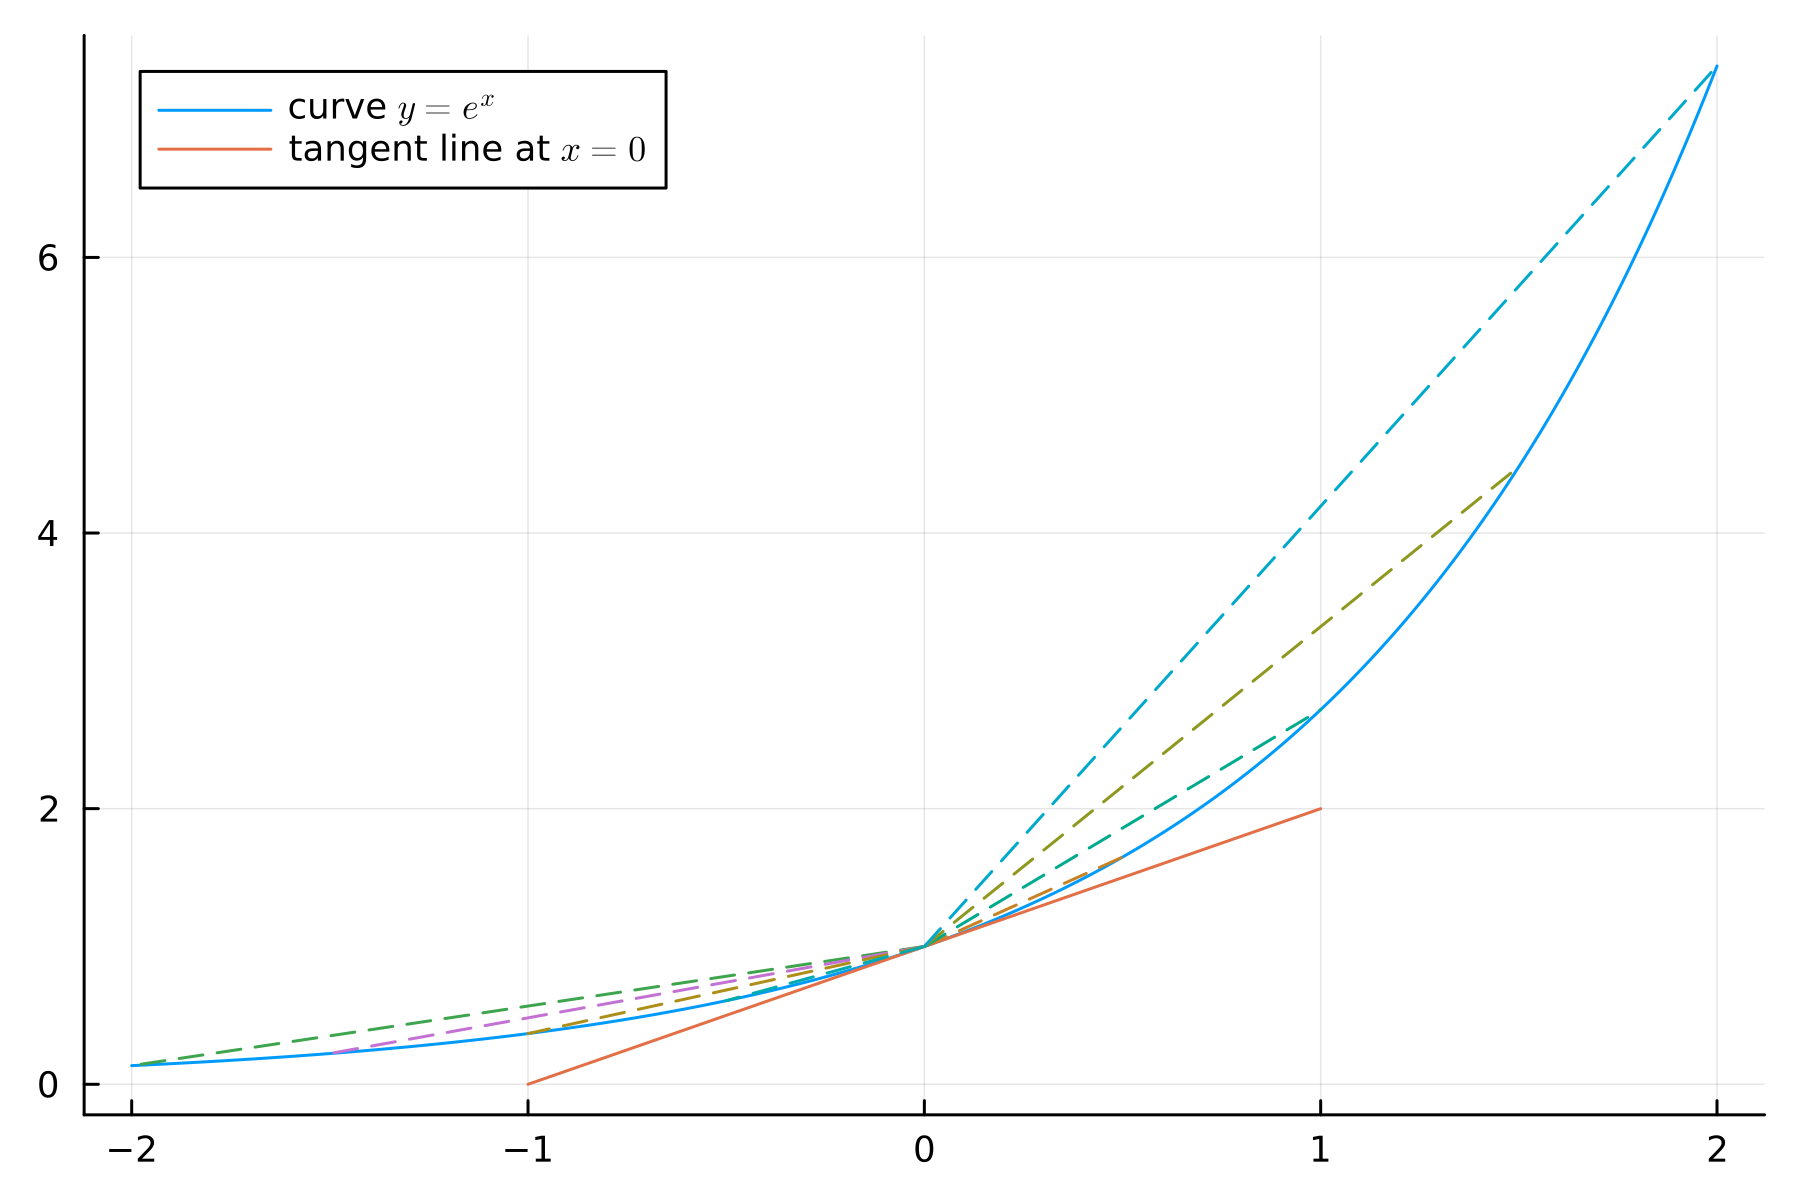
\includegraphics[scale=0.2]{figures/secant-lines-and-a-tangent-line.png}
    \caption{Secant lines and a tangent line of curve $y=e^x$.}
    \label{fig:1}
\end{figure}

\noindent All secant lines have a common point of intersection, $(0, 1)$. And as the other intersection point gets closer and closer to $(0, 1)$, the slope of the secant line tends to converge to some number. This number, the limiting slope, is precisely the \textbf{derivative} of this curve/function at $x=0$, which we shall soon define. We can draw a straight line passing through the point $(0,1)$ with the limiting slope. This line is then called the tangent of the curve at point $(0,1)$, as illustrated in Figure~\ref{fig:1}. 

\begin{definition}
    Let $f$ be defined on an open interval $(a, b)$, and let $c \in (a, b)$ an interior point. Then $f$ is said to be \textbf{differentiable}\index{differentiable functions} at $c$ if the limit 
    \begin{align*}
        \lim_{x \to c} \frac{f(x) - f(c)}{x - c}        
    \end{align*}
    exists. This limit, denoted by $f^\prime(c)$, is called the \textbf{derivative} \index{derivative} of $f$ at point $c$.
\end{definition}

If $f^\prime(c)$ exists $\forall c \in I$ for some interval $I$, then we can define a function $f^\prime$ on $I$, which is called the derivative of $f$. Here the word \textit{derivative} means a function instead of just a number. 

%------------------------------

The definition of derivatives we present here involves the limit obtained by letting one point approach the other one, $x \to c$. For computational convenience, we can treat the derivative of $f$ at $c$ as the limit of the fraction $[ f(c+h) - f(c) ] / h$ as $h \to 0$. That is, the limit is reached when the distance between points $x$ and $c$, $h = \abs{x-c}$, is small. The following proposition states this idea formally.

\begin{proposition} \label{pro:1}
    Let $f$ be defined on $(a, b)$. Then $f$ is differentiable at $c \in (a, b)$ if and only if 
    \begin{align}
        \lim_{h \to 0} \frac{f(c+h) - f(c)}{h} 
        \label{eq:3}
    \end{align}
    exists. In that case, $f^\prime(c) = \lim_{h \to 0} [ f(c+h) - f(c) ] / h$.
\end{proposition}

\begin{proof}
    Suppose $f$ is differentiable at $c$. For an arbitrary $\varepsilon > 0$, there exists $\delta > 0$ such that 
    \begin{align*}
        \abs{x - c} < \delta
        \implies \abs{\frac{f(x) - f(c)}{x - c} - f^\prime(c)} < \varepsilon
    \end{align*}
    Let number $h$ be such that $\abs{h} < \delta$. Then since $\abs{(c+h) - c} = \abs{h} < \delta$, we have 
    \begin{align*}
        \abs{\frac{f(c+h) - f(h)}{h} - f^\prime(c)}
        = \abs{\frac{f(c+h) - f(h)}{(c+h) - c} - f^\prime(c)} < \varepsilon
    \end{align*}
    This implies the limit \eqref{eq:3} exists, and it equals $f^\prime(c)$.

    Conversely, suppose the limit \eqref{eq:3} exists, say it equals $L$. Then for $\varepsilon > 0$ there exists $\delta > 0$ such that 
    \begin{align*}
        \abs{h} < \delta
        \implies \abs{\frac{f(c+h) - f(c)}{h} - L} < \varepsilon
    \end{align*}
    Choose $x$ such that $\abs{x - c} < \delta$, we have 
    \begin{align*}
        \abs{
            \frac{f(x) - f(c)}{x - c} - L
        } = \abs{
            \frac{f(c + (x - c)) - f(c)}{x - c} - L
        } < \varepsilon
    \end{align*}
    Therefore, the limit $[f(x) - f(c)]/(x - c)$ exists, which is equal to $L$. By the definition of derivatives, $f$ is differentiable at $c$, and $f^\prime(c) = L$.
\end{proof}

\begin{exercise}
    Calculate the derivative of $e^x$ at $x = 0$. 

    \noindent [Hint: You may use the fact $e^x = \sum_{n=0}^\infty \frac{x^n}{n!} =  1 + x + \frac{1}{2} x^2 + \frac{1}{6} x^3 + \cdots$.]
\end{exercise}

\begin{exercise}
    Calculate the derivative of
    \begin{align*}
        f(x) 
        = x^2 \sin \frac{1}{x^2} \ind\{x \neq 0\}
        = \begin{cases}
            x^2 \sin \frac{1}{x^2} &x \neq 0 \\ 
            0 &x=0
        \end{cases}
    \end{align*}
    at $x = 0$.
    \label{ex:1}
\end{exercise}

\begin{solution}
    We have 
    \begin{align*}
        \frac{f(0+h) - f(0)}{h}
        = h \sin \frac{1}{h^2}
    \end{align*}
    Note the limit of the above expression is zero as $h \to 0$ by Proposition~\ref{pro:2} since $\lim_{h\to 0} h = 0$ and $\sin (1/h^2)$ is bounded by $1$. Hence, $f^\prime(0) = 0$ by Proposition~\ref{pro:1}.

    The graph of $f(x)$ is shown in Figure~\ref{fig:2}. As we can see, $f(x)$ is clamped between curves $y=x^2$ and $y=-x^2$ with the same tangents $y=0$ at $x=0$. And we have shown $f^\prime(0)=0$, which means that the tangent of $f(x)$ is also $y=0$ at $x=0$. What conjecture can you make?

    \begin{figure}[ht]
        \centering
        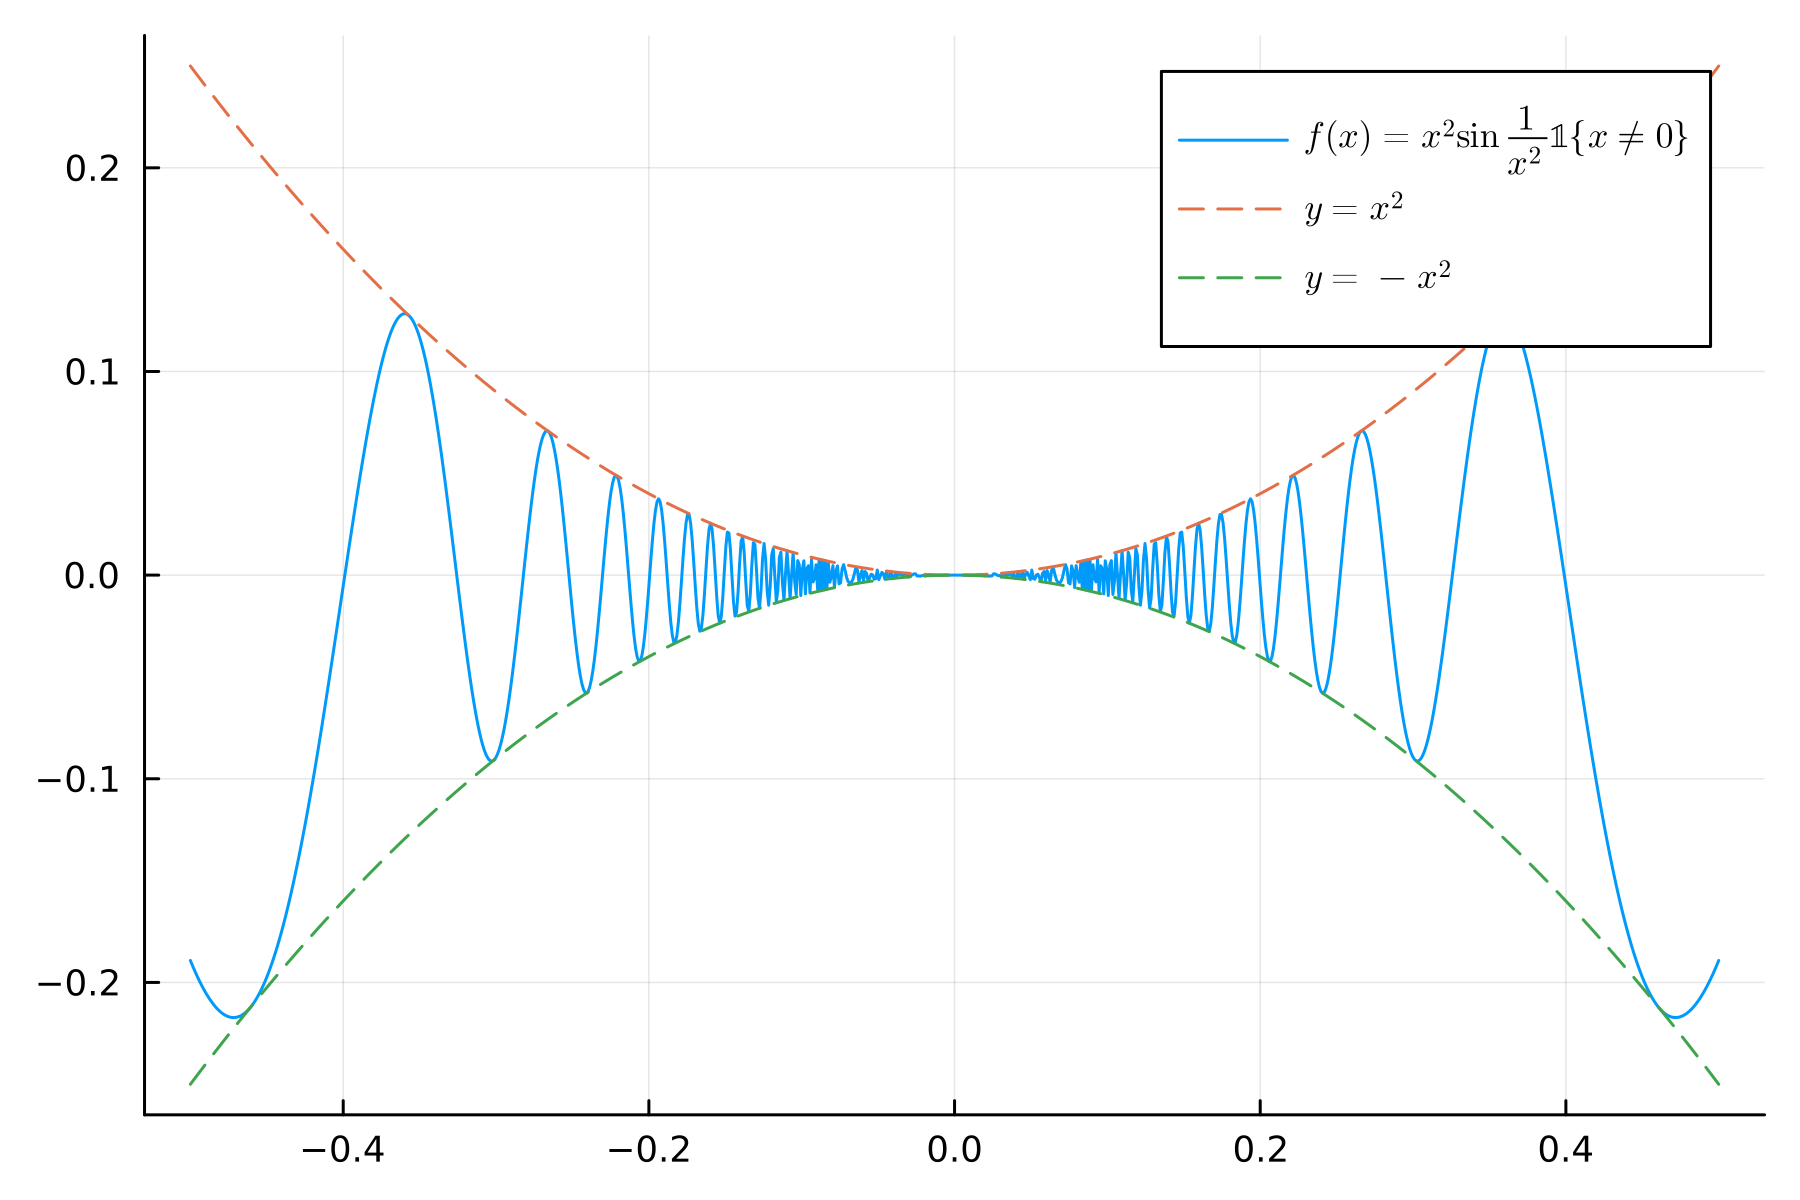
\includegraphics[scale=0.2]{figures/graph-001.png}
        \caption{Graph of $f(x) = x^2 \sin \frac{1}{x^2} \ind\{x \neq 0\}$.}
        \label{fig:2}
    \end{figure}

    Moreover, we observe that $f(x)$ crosses its tangent line at $x=0$ infinitely many times. This example shows that the tangent line does not have to touch the curve only at one point.
\end{solution}

%------------------------------

\subsection{One-Sided Derivatives and Infinite Derivatives}

So far, the point at which the derivative is defined has to be an \textit{interior} point. Sometimes, we are required to consider the derivatives at the endpoints of the interval. For example, as we shall see in more detail in Chapter~\ref{chap:1}, we need to take the derivative of function $F(x) = \int_a^x f(t) \mathrm{d}t$ at $x=a$. Hence, we are motivated to define the \textbf{one-sided derivatives}\index{one-sided derivatives}. 

If we consider the derivative of $f$, $f^\prime$ as a function, then $f^\prime(x)$ may tend to infinity as $x$ approaches an endpoint. In addition, sometimes we need to interpret the meaning of vertical tangent lines. This leads to the definition of \textbf{infinite derivatives}\index{infinite derivative}.

\begin{definition}
    Let $f$ be defined on a closed interval $I$. Suppose $f$ is continuous at point $c \in I$. Then $f$ is said to have a \textbf{right-hand derivative}\index{right-hand derivative} at $c$ if the right-hand limit 
    \begin{align*}
        \lim_{x \to c^{+}} \frac{f(x) - f(c)}{x - c}
    \end{align*}
    exists as a finite number, or the limit is $\infty$ or $-\infty$. This right-hand derivative shall be denoted by $f^\prime_{+}(c)$. The \textbf{left-hand derivative}\index{left-hand derivative}, denoted by $f^\prime_{-}(c)$, is defined similarly. In addition, if $c$ is an interior point, and $f^\prime_{+}(c) = f^\prime_{-}(c) = \infty$, then we write $f^\prime(c) = \infty$. $f^\prime(c) = -\infty$ is similarly defined.
\end{definition}

\begin{remark}
    Note that though we write $f^\prime(c) = \infty$ or $f^\prime(c) = -\infty$, we do not say $f$ is differentiable there.
\end{remark}

It is not very intuitive to imagine, at first thought, a continuous function having infinite derivatives. But there are quite a lot of such examples.

\begin{example}
    The first example is constructed by cutting a circle in the middle. If we cut a circle in half and stick the lower half to the right of the upper one, then we have a function with a vertical tangent line in the middle. The explicit expression of this function is 
    \begin{align*}
        f(x) = \begin{cases}
            \sqrt{1 - (x-1)^2} &0 \leq x \leq 2 \\ 
            - \sqrt{1 - (x-3)^2} &2 < x \leq 4
        \end{cases}
    \end{align*}

    \begin{figure}[ht]
        \centering
        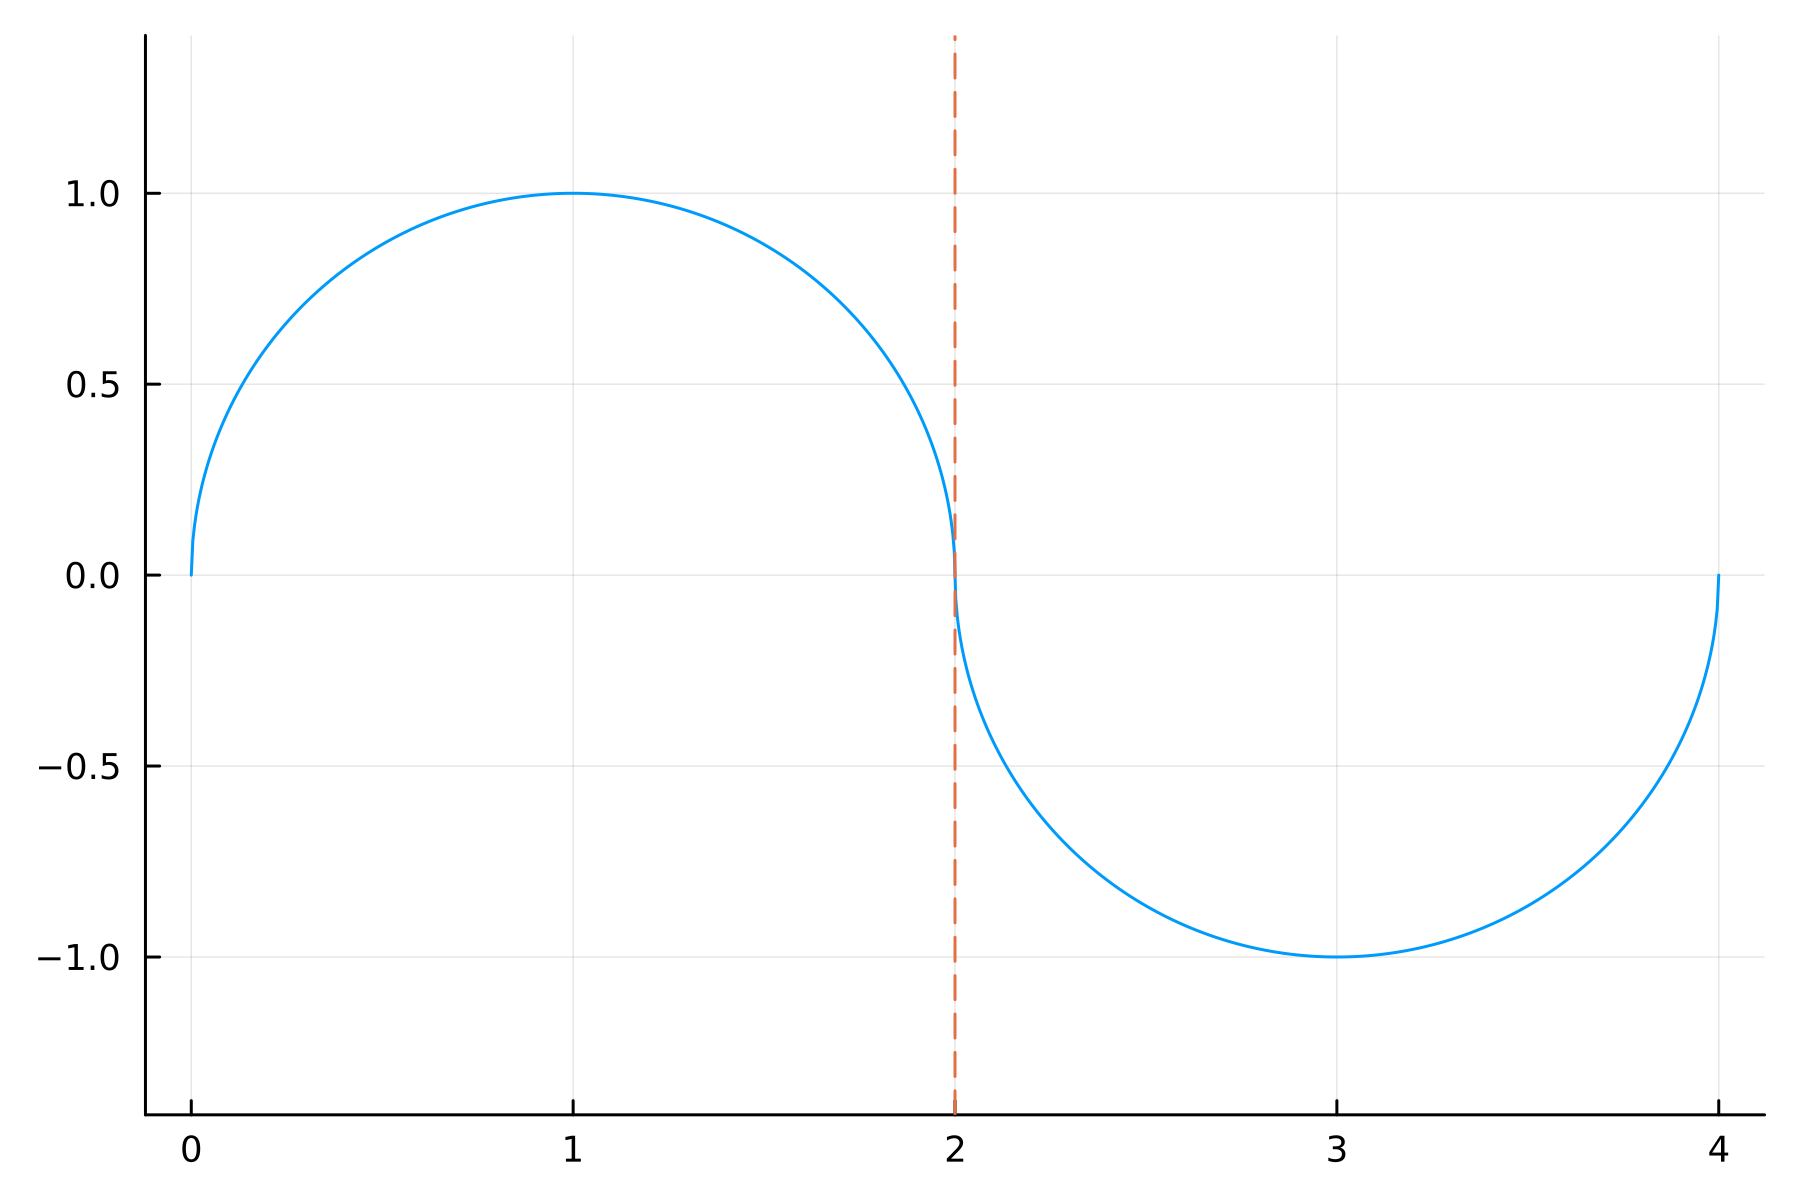
\includegraphics[scale=0.2]{figures/graph-002.png}
        \caption{Graph of $f(x) = \sqrt{1-(x-1)^2}\ind\{0 \leq x \leq 2\} - \sqrt{1-(x-3)^2}\ind\{2 < x \leq 4\}$.}
    \end{figure}

    \noindent The function is continuous and one can show that $f^\prime(2) = -\infty$.
    \label{eg:1}
\end{example}

\begin{example}
    The following next example includes both positive and negative intuitive derivatives, and a point at which the right and left-hand side derivatives are $\infty$ and $-\infty$, respectively. Consider the function 
    \begin{align*}
        f(x) = \sqrt[3]{x^2 (x-1) (x-2)}
    \end{align*}
    Its graph is shown in Figure~\ref{fig:3}.

    \begin{figure}[ht]
        \centering
        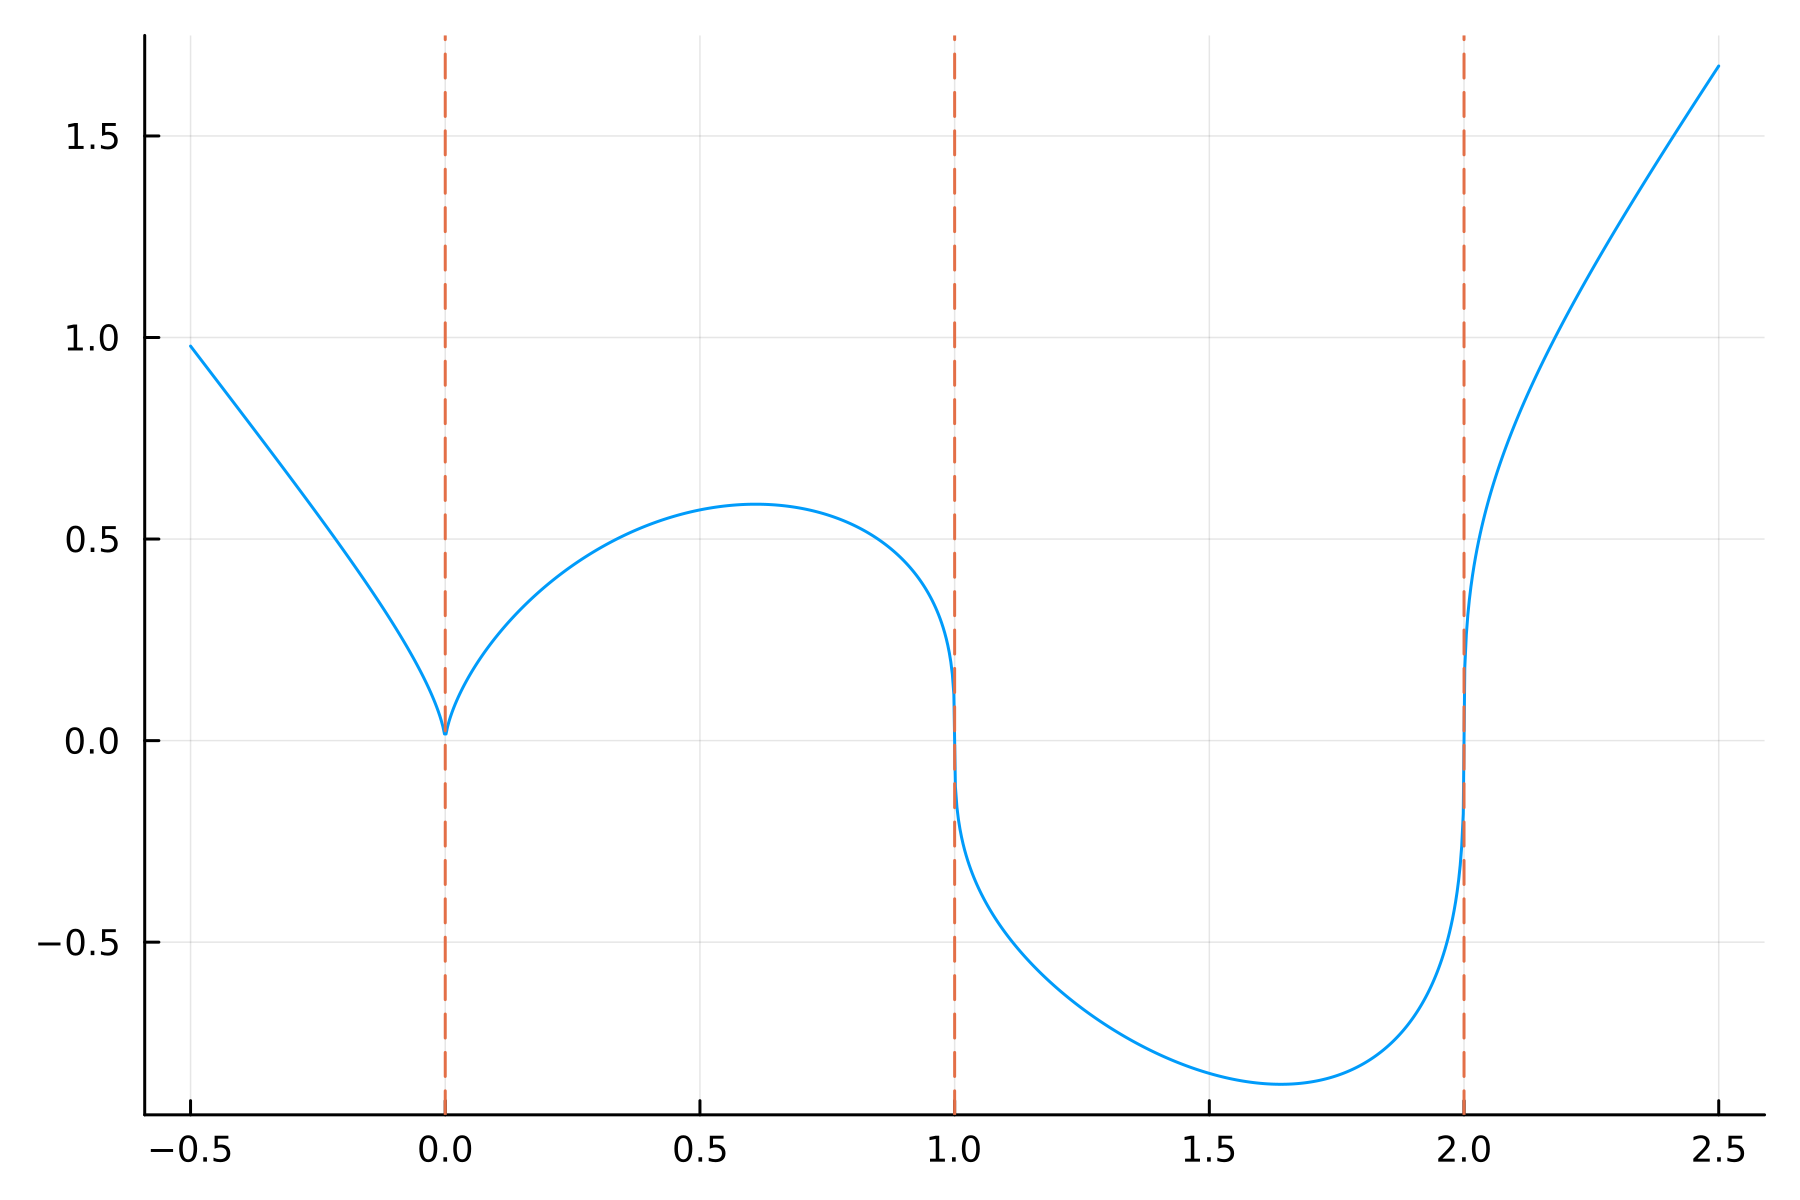
\includegraphics[scale=0.2]{figures/graph-003.png}
        \caption{Graph of $f(x) = \sqrt[3]{x^2 (x-1) (x-2)}$.}
        \label{fig:3}
    \end{figure}    

    It is an exercise to show $f^\prime(1) = -\infty$ and $f^\prime(2) = \infty$. We now consider the one-sided derivatives at $x = 0$. We have 
    \begin{align*}
        \frac{f(x) - f(0)}{x - 0}
        = \sqrt[3]{\frac{(x-1)(x-2)}{x}}
    \end{align*}
    Letting $x \to 0^{+}$ leads to $f^\prime_{+}(0) = \infty$, while $x \to 0^{-}$ yields $f^\prime_{-}(0) = -\infty$. Hence, we say the derivative of $f$ does not exist at $x = 0$.
    \label{eg:2}
\end{example}

%------------------------------

\section{Derivatives and Continuity}

The next theorem helps to reduce some theorems on derivatives to theorems on continuity.

\begin{theorem} \label{thm:1}
    Let $f$ be a function defined on $(a, b)$, and $c \in (a, b)$ a fixed point in that interval. We have the following statements:
    \begin{enumerate}
        \item If $f$ is differentiable at $c$, then there exists a function $\phi$ on $(a, b)$ which is continuous at $c$, and satisfies 
        \begin{align}
            f(x) - f(c) = (x - c) \phi(x)
            \quad \forall x \in (a, b)
            \label{eq:1}
        \end{align}
        And $f^\prime(c) = \phi(c)$.
        \item Conversely, if there exists a function $\phi$ on $(a, b)$ which is continuous at $c$, and satisfies \eqref{eq:1}, then $f$ is differentiable at $c$ with $f^\prime(c) = \phi(c)$.
    \end{enumerate}
\end{theorem}

The function $\phi$ is precisely the slope of function $f$'s secant line.

\begin{proof}
    (Proof of 1) Suppose $f$ is differentiable at $c$. Define 
    \begin{align*}
        \phi(x) = \frac{f(x) - f(c)}{x - c}, 
        \quad x \neq c
        \quad\text{and}\quad 
        \phi(c) = \lim_{x \to c} \frac{f(x) - f(c)}{x - c}
    \end{align*}
    Note that $\phi(c)$ is well-defined since the limit (which equals $f^\prime(c)$) indeed exists by the definition of the derivative of $f$ at $c$. Notice also that by defining function $\phi$ in this way, it is automatically continuous at $c$. And of course, the equation \eqref{eq:1} holds.

    (Proof of 2) It follows from \eqref{eq:1} that 
    \begin{align*}
        \phi(x) = \frac{f(x) - f(c)}{x - c}
        \quad \forall x \neq c
    \end{align*}
    Since $\phi$ is continuous at $c$, by sending $x \to c$, we have 
    \begin{align*}
        \phi(c) = \lim_{x \to c} \phi(x)
        = \lim_{x \to c} \frac{f(x) - f(c)}{x - c}
    \end{align*}
    This implies $f$ is differentiable at $c$, and $f^\prime(c) = \phi(c)$.
\end{proof}

%------------------------------

With the help of Theorem~\ref{thm:1}, we can easily show that $f$ must be continuous at $c$ if it is differentiable there.

\begin{theorem} \label{thm:2}
    Let $f$ be defined on $(a, b)$. If $f$ is differentiable at $c \in (a, b)$, then it is continuous at $c$.
\end{theorem}

\begin{proof}
    By Theorem~\ref{thm:1}, there exists a function $\phi$ on $(a, b)$ such that $\phi$ is continuous at $c$, and
    \begin{align}
        f(x) - f(c) = (x - c) \phi(x)
        \quad \forall x \in (a, b)
        \label{eq:2}
    \end{align}
    Since the limit of the right-hand side in \eqref{eq:2} exists as $x \to c$, the limit of the left-hand side also exists, and 
    \begin{align*}
        \lim_{x \to c} f(x) - f(c)
        = \lim_{x \to c}(x - c) \phi(x)
        = 0
    \end{align*}
    This implies 
    \begin{align*}
        \lim_{x \to c} f(x) = f(c)
    \end{align*}
    Hence, $f$ is continuous at $c$.
\end{proof}

%------------------------------

\section{Computing Derivatives}

It is difficult in practice to compute the derivative of any function only using the definition. In this section, we shall introduce some theorems and standard rules that are helpful with computation. If one knows the derivatives of elementary functions (e.g., $x^a$, $e^x$, $\ln x$, $\sin x$, $\cos x$, etc.), then by applying these theorems, one should be able to compute the derivatives of any functions that are built up out of elementary functions using summations, differences, products, quotients, and compositions.

\begin{note}
    In fact, these so-called elementary functions are not elementary at all. We shall present their definitions as well as their derivatives rigorously in later chapters.
\end{note}

%------------------------------

\subsection{Algebra of Derivatives}

%------------------------------

\begin{theorem}
    Suppose $f$ and $g$ are defined on $(a, b)$ and are both differentiable at $c \in (a, b)$. Then the functions $f + g$, $f - g$, $fg$ are also differentiable at $c$. If $g(c) \neq 0$, then the quotient $f / g$ is also differentiable at $c$. And the formulas of their derivatives are given by 
    \begin{enumerate}
        \item $(f \pm g)^\prime(c) = f^\prime(c) \pm g^\prime(c)$, 
        \item $(f g)^\prime(c) = f^\prime(c) g(c) + f(c) g^\prime(c)$, 
        \item $(f / g)^\prime(c) = \frac{f^\prime(c) g(c) - f(c) g^\prime(c)}{ g^2(c) }$, provided $g(c) \neq 0$.
    \end{enumerate}
\end{theorem}

\begin{remark}
    One might be worried about the possibility that the quotient $f / g$ may only be defined at point $c$ if we only require $g(c) \neq 0$. Then how can we say $f / g$ is differentiable at some point? However, the condition that $g$ is differentiable at $c$ implicitly implies that $g(x) \neq 0$ for $x$ in some interval about $c$ if we assume $g(c) \neq 0$. Take a few seconds and think about why this is true. Note that $g$ is continuous at $c$ by Theorem~\ref{thm:2}. Then, if $g(c) \neq 0$, by the continuity, $g$ is also nonzero in some neighborhood of $c$. Hence, in this case, $f / g$ is actually well-defined in an interval instead of at just one point.
\end{remark}

The proof we present here is done by exploiting Theorem~\ref{thm:1}, and it may differ from a traditional proof that is solely based on the definition.

\begin{proof}
    Since $f$ and $g$ are differentiable at $c$. It follows from Theorem~\ref{thm:1} that there exists functions $\phi_1$ and $\phi_2$ on $(a, b)$ that are continuous at $c$, and satisfy
    \begin{align}
        f(x) - f(c) = (x - c) \phi_1^\prime(x) \label{eq:4}
    \end{align}
    \begin{align}
        g(x) - g(c) = (x - c) \phi_2^\prime(x) \label{eq:5}  
    \end{align}
    with
    \begin{align}
        \phi_1 (c) = f^\prime(c)
        \quad \text{and} \quad 
        \phi_2 (c) = g^\prime(c)
        \label{eq:6}
    \end{align}

    (Proof of 1) Applying \eqref{eq:4} and \eqref{eq:5} to $(f \pm g)(x) - (f \pm g)(c)$, we have 
    \begin{align*}
        (f \pm g)(x) - (f \pm g)(c)
        = (x - c) (
            \phi_1(x) \pm \phi_2(x)
        )
    \end{align*}
    Since $\phi_1(x) \pm \phi_2(x)$ is continuous at $c$, $(f \pm g)$ is differentiable at $c$ by Theorem~\ref{thm:1}. Then by applying \eqref{eq:6}, we obtain
    \begin{align*}
        (f \pm g)^\prime (c)
        = \phi_1(c) \pm \phi_2(c)
        = f^\prime(c) \pm g^\prime(c)
    \end{align*}

    (Proof of 2) Again by applying \eqref{eq:4} and \eqref{eq:5}, we have 
    \begin{align*}
        (f g)(x) - (f g)(c)
        = (x - c) [
            \phi_1(x) g(c) 
            + f(c) \phi_2(x)
            + (x - c) \phi_1(x) \phi_2(x)
        ]
    \end{align*}
    after a few steps of algebraic calculation. It then follows from Theorem~\ref{thm:1} that $f g$ is differentiable at $c$ since the function 
    \begin{align*}
        \phi_1(x) g(c) 
            + f(c) \phi_2(x)
            + (x - c) \phi_1(x) \phi_2(x)
    \end{align*}
    is continuous at $c$. And 
    \begin{align*}
        (f g)^\prime (c)
        = \phi_1(c) g(c) 
        + f(c) \phi_2(c)
        + (c - c) \phi_1(c) \phi_2(c)
        = f^\prime(c) g(c) + f(c) g^\prime(c)
    \end{align*}

    (Proof of 3) Note that the quotient $(f / g)$ can be regarded as a product of $f$ and $1 / g$. Hence, we are going to show $1/g$ is differentiable at $c$, and then apply statement 2, which we have just proved, to conclude the proof. As explained in the remark of this theorem, $1/g$ is well-defined in a neighborhood of $c$. It follows from \eqref{eq:5} that 
    \begin{align*}
        \frac{1}{g(x)} - \frac{1}{g(c)}
        = (x - c) \frac{-\phi_2(x)}{g(x)g(c)}
    \end{align*}
    Since $-\phi_2(x) / [g(x)g(c)]$ is continuous at $c$, we conclude from Theorem~\ref{thm:1} that $1/g$ is differentiable at $c$, and 
    \begin{align*}
        \left( \frac{1}{g} \right)^\prime (c)
        = \frac{-\phi_2(c)}{g(c)g(c)}
        = \frac{-g^\prime(c)}{g^2(c)}
    \end{align*}
    Then by applying statement 2, we conclude that $f / g$ is also differentiable at $c$ with 
    \begin{align*}
        (f / g)^\prime(c) = \frac{f^\prime(c) g(c) - f(c) g^\prime(c)}{ g^2(c) }
    \end{align*}
\end{proof}

%------------------------------

\subsection{The Chain Rule}

Taking compositions is a more fundamental and natural way of combining two functions apart from summations, products, etc. The next result, the \textbf{chain rule}\index{chain rule}, provides a method of computing the derivative of a composite function.

\begin{theorem} \label{thm:4}
    Let $f$ be a function defined on an open interval $I$, and $g$ a function defined on $f(I)$. We consider the composite function $g \circ f$. If $f$ is differentiable at $c \in I$, $f(c)$ is an interior of $f(I)$, and $g$ is differentiable at $f(c)$, then $g \circ f$ is differentiable at $c$ with 
    \begin{align}
        (g \circ f)^\prime (c)
        = g^\prime(f(c)) f^\prime(c)
        \label{eq:9}
    \end{align}
\end{theorem}

With the help of Theorem~\ref{thm:1}, we can reduce the proof of this theorem to that of Theorem~\ref{thm:3}.

\begin{proof}
    Since $f$ is differentiable at $c$, using Theorem~\ref{thm:1}, we have 
    \begin{align}
        f(x) - f(c) = (x-c) \phi_1(x)
        \quad \forall x \in I
        \label{eq:10}
    \end{align}
    where $\phi_1$ is some function that is continuous at $c$ with $\phi_1(c) = f^\prime(c)$. Using the same argument, since $g$ is differentiable at $f(c)$, we have 
    \begin{align}
        g(y) - g(f(c)) = (y-f(c)) \phi_2(y)
        \quad \forall y \in f(I)
        \label{eq:11}
    \end{align}
    where $\phi_2$ is some function that is continuous at $f(c)$ with $\phi_2(c) = g^\prime(f(c))$. Replace $y$ with $f(x)$ in \eqref{eq:11} yields 
    \begin{align*}
        g(f(x)) - g(f(c)) = (f(x)-f(c)) \phi_2(f(x))
        \quad \forall x \in I
    \end{align*}
    Then by replacing $f(x)-f(c)$ with the right-hand side of \eqref{eq:10}, we have 
    \begin{align*}
        g(f(x)) - g(f(c)) = (x-c) \phi_1(x) \phi_2(f(x))
        \quad \forall x \in I
    \end{align*}
    Note that $\phi_2(f(x))$ is continuous at $c$ by Theorem~\ref{thm:3}. And the product $\phi_1(x) \phi_2(f(x))$ is also continuous. This implies $f \circ f$ is differentiable at $c$ by Theorem~\ref{thm:1}. And its derivative at $x = c$ equals
    \begin{align*}
        (g \circ f)^\prime(c)
        = \phi_1(c) \phi_2(f(c))
        = f^\prime(c) g^\prime(f(c))
    \end{align*}
    which is exactly \eqref{eq:9}.
\end{proof}

\begin{exercise}
    Calculate the derivative of
    \begin{align*}
        g(x) = x \sin \frac{1}{x} \ind\{x \neq 0\}
    \end{align*}
    for $x \neq 0$. Does the derivative exist at $x = 0$?
    \label{ex:2}
\end{exercise}

\begin{exercise}
    Calculate the derivative of 
    \begin{align*}
        f(x) = x^2 \sin \frac{1}{x^2} \ind\{x \neq 0\}
    \end{align*}
    for all $x \in \R$. Recall we have already calculated its derivative at $x = 0$ in Exercise~\ref{ex:1}, which is $f^\prime(0) = 0$.

    \noindent [Hint: Make use of the result in Exercise~\ref{ex:2} and the chain rule (Theorem~\ref{thm:4}).]
    \label{ex:3}
\end{exercise}

%------------------------------

\section{The Mean Value Theorem} 

%------------------------------

\subsection{Local Extrema}

\par One may be familiar with the fact that if the derivative of function $f$ is positive at some point, i.e., $f^\prime(c) > 0$, then $f$ is increasing near $c$, and if $f^\prime(c) < 0$, it is decreasing. However, we can extend this result a little further for we have defined one-sided and infinite derivatives.

\begin{theorem} \label{thm:14}
    Let $f$ be defined on a subset $A \subseteq \R$ and $c \in A$. If $f^\prime_+(c) > 0$, possibly $f^\prime_+(c) = \infty$, then there exists a half-open ball $(c, c+\delta) \subseteq A$ in which
    \begin{align}
        x > c \implies f(x) > f(c)
        \label{eq:12}
    \end{align}
    Similarly, if $f^\prime_{-}(c) > 0$, then $\exists (c-\delta, c) \subseteq A$ in which
    \begin{align*}
        x < c \implies f(x) < f(c)
    \end{align*}
    Analogous results hold if we instead assume $f^\prime_{+}(c) < 0$ or $f^\prime_{-}(c) < 0$.
\end{theorem}

\begin{proof}
    We only prove \eqref{eq:12} since the proofs of the rest of the results are similar. First suppose $f^\prime_{+}(c) < \infty$. Because the right-hand limit exists, and it equals $f^\prime_{+}(c)$, there exists $\delta > 0$ such that
    \begin{align*}
        \abs{
            \frac{f(x) - f(c)}{x - c}
            - f^\prime_{+}(c)
        } < \frac{f^\prime_{+}(c)}{2}
        \quad \forall x \in (c, c+\delta)
    \end{align*}
    This implies
    \begin{align*}
        \frac{f(x) - f(c)}{x - c} > \frac{f^\prime_{+}(c)}{2} > 0
        \quad \forall x \in (c, c+\delta)
    \end{align*}
    Then $f(x) > f(c)$ provided $x > c$ since they have the same sign.
    
    We also need to consider $f^\prime_{+}(c) = \infty$. Because the limit is infinity, there exists $\delta > 0$ such that the following fraction exceeds any predetermined number, in particular,
    \begin{align*}
        \frac{f(x) - f(c)}{x - c} > 0
        \quad \forall x \in (c, c+\delta)
    \end{align*}
    One can instead choose any large number (non-negative of course, to prove this theorem). This completes the proof since both the numerator and denominator share the same sign.
\end{proof}

\par The following corollary is the version that is more familiar to the reader and is more common in practice.

\begin{corollary} \label{cor:1}
    Let $f$ be defined on $(a, b)$, and $c \in (a, b)$ an interior point. If $f^\prime(c) > 0$, possibly $f^\prime(c) = \infty$, then there exists an open ball $B_\delta(c) \subseteq (a, b)$ in which
    \begin{align}
        x > c \implies f(x) > f(c)
        \quad \text{and} \quad 
        x < c \implies f(x) < f(c)
        \label{eq:14}
    \end{align}
    An analogous result holds if $f^\prime(c) < 0$.
\end{corollary}

\begin{exercise}
    Prove Corollary~\ref{cor:1} assuming $f^\prime(c) < \infty$ using Theorem~\ref{thm:1}.
\end{exercise}

\begin{solution}
    It follows from Theorem~\ref{thm:1} that 
    \begin{align}
        f(x) - f(c) = (x - c) \phi(x)
        \quad \forall x \in (a, b)
        \label{eq:13}
    \end{align}
    where $\phi(x)$ is continuous at $c$ with $\phi(c) = f^\prime(c) > 0$. Since $\phi(c) > 0$ and it is continuous there, there exists some neighborhood $B_\delta(c) \subseteq (a, b)$ such that $\phi(x) > 0 \; \forall x \in B_\delta(c)$. And then \eqref{eq:14} follows from \eqref{eq:13}.
\end{solution}

%------------------------------

\par The \textbf{local extremum}\index{local extremum} of a function is the largest or smallest value within some \textit{open ball}.

\begin{definition}
    Let $f$ be a real-valued function defined on a subset $A$ of a metric space $(X, d)$, and suppose $p \in A$. Then $f$ is said to have a \textbf{local maximum}\index{local maximum} at $p$ if 
    \begin{align*}
        f(x) \leq f(p)
        \quad \forall x \in B_\delta(p) \cap A
    \end{align*} 
    for some open ball $B_\delta(p)$. An analogous definition exists for \textbf{local minimum}\index{local minimum}.
\end{definition}

%------------------------------

\par The reader should be very familiar with the exercise of finding a local extremum by solving the equation in which the derivative vanishes. The following Theorem is the theory behind that.

\begin{theorem} \label{thm:5}
    Let $f$ be defined on $(a, b)$, and suppose $f$ has a local extremum at an interior point $c \in (a, b)$. If $f^\prime(c)$ exists as a finite or infinite number, then $f^\prime(c) = 0$.
\end{theorem}

\begin{remark}
    Since the conclusion is $f^\prime(c) = 0$, we may as well just assume $f$ is differentiable at $c$. The reason why we suppose $f^\prime(c)$ exists is that it makes the assumption somewhat looser.
\end{remark}

\begin{proof}
    We shall prove by contradiction. Assume $f^\prime(c) \neq 0$, then either $f^\prime(c) > 0$ or $f^\prime(c) < 0$. (We do not exclude the possibilities that $f^\prime(c) = \infty$ or $f^\prime(c) = -\infty$.) If $f^\prime(c) > 0$, then follows from Corollary~\ref{cor:1} that there acts some open ball $B_\delta(c)$ in which $f(x) > f(c)$ for $x > c$ and $f(x) < f(c)$ for $x < c$. This contradicts the fact that $f(c)$ is a local extremum. Similarly, $f^\prime(c) < 0$ will also lead to a contradiction. 
\end{proof}

\par The converse of this Theorem is not true. 

\begin{example}
    Consider $f(x) = x^3$. Its derivative is $f^\prime(x) = 3x^2$. We note that $f^\prime(0) = 0$. But it is clear that $f(0) = 0$ is neither a local maximum nor a local minimum. In fact, $f(x)$ does not have any local extremum.
\end{example}

\begin{exercise}
    Recall the function 
    \begin{align*}
        f(x) = x^2 \sin \frac{1}{x^2} \ind\{x \neq 0\}
    \end{align*}
    defined in Exercise~\ref{ex:1}. Show that $f(0)$ is not a local extremum. Recall we have shown that $f^\prime(0) = 0$. This is another example that the converse of Theorem~\ref{thm:5} does not hold.
\end{exercise}

\par Moreover, it should be emphasized that we conclude in Theorem~\ref{thm:5} that $f^\prime(c) = 0$ under the condition that $f^\prime(c)$ exists. $f(c)$ may be a local extremum without having a derivative there.

\begin{example}
    The simplest example is $f(x) = \abs{x}$. Note that $f(0) = 0$ is a local minimum. But the derivative does not exist at $x = 0$ since $f^\prime_{+}(0) = 1 \neq -1 = f^\prime_{-}(0)$.
\end{example}

%------------------------------

\subsection{Rolle's Theorem and Mean Value Theorem}

\par If a function starts from point $a$ and ends at point $b$ with the same level of height as its initial position, then there must be a turning point somewhere in between. 

\begin{theorem}[Rolle] \label{thm:9}
    Let $f$ be defined on $[a, b]$. Suppose $f^\prime(x)$ exists (as finite or infinite number) for each $x \in (a, b)$, and $f$ is continuous at the endpoints $a$ and $b$. If $f(a) = f(b)$, then there exists $c \in (a, b)$ such that 
    \begin{align*}
        f^\prime(c) = 0
    \end{align*}
\end{theorem}

\begin{proof}
    If $f$ is a constant function, i.e., $f(x) = f(a) = f(b) \; \forall x \in [a, b]$, then the conclusion is trivial since $f^\prime(x) = 0 \; \forall x \in (a, b)$.

    We now suppose $f$ is non-constant. We know that $f$ is continuous on $[a, b]$ since $f^\prime$ exists throughout $(a, b)$ and $f$ is continuous at endpoints. It then follows from Theorem~\ref{thm:6} that $f$ attains its maximum and minimum on $[a, b]$. Because we assume $f$ is non-constant and $f(a) = f(b)$, at least one of the maximum and the minimum of $f$ is reached at an interior point $c \in (a, b)$. Note that $f(c)$ is a global extremum, and of course also a local extremum. Then by applying Theorem~\ref{thm:5}, we conclude $f^\prime(c) = 0$.
\end{proof}

\begin{example}
    Review Example~\ref{eg:1}. Note that $f(0) = f(4) = 0$. And the derivative vanishes at $x = 1$ and $x = 3$. 
\end{example}

%------------------------------

\par The \textbf{mean value theorem}\index{mean value theorem} is a generalization of Rolle's theorem. Roughly speaking it says $f$ has a derivative value that equals the slope of the secant line joining two endpoints of the graph of $f$. The mean value theorem itself can be treated as a special case of an even more generalized version, the \textbf{generalized mean value theorem}\index{generalized mean value theorem} (Theorem~\ref{thm:7}).

\begin{theorem}[Mean Value Theorem] \label{thm:8}
    Suppose $f$ has a derivative (finite or infinite) at each point of $(a, b)$, and suppose $f$ is continuous at endpoints $a$ and $b$. Then there exists $c \in (a, b)$ such that 
    \begin{align*}
        f(b) - f(a) = f^\prime(c) (b - a)
    \end{align*}
\end{theorem}

\begin{theorem}[Generalized Mean Value Theorem] \label{thm:7}
    Let $f$ and $g$ be two functions, each having a derivative (finite or infinite) at each point in $(a, b)$. Suppose $f$ and $g$ are both continuous at endpoints $a$ and $b$, and $f^\prime(x)$ and $g^\prime(x)$ do not assume infinite values simultaneously. Then there exists $c \in (a, b)$ such that 
    \begin{align}
        f^\prime(c) [g(b) - g(a)]
        = g^\prime(c) [f(b) - f(a)]
        \label{eq:15}
    \end{align} 
\end{theorem}

\begin{remark}
    By taking $g(x) = x$, this theorem reduces to the standard mean value theorem, Theorem~\ref{thm:8}.
\end{remark}

\par Though it is a generalized version of the mean value theorem, and hence Rolle's theorem, it can be proved easily using Rolle's theorem by constructing a function out of $f$ and $g$.

\begin{proof}
    Define 
    \begin{align*}
        \psi(x) = f(x)[g(b) - g(a)] - g(x) [f(b) - f(a)]
    \end{align*}
    It is clear that $\psi$ is continuous on $[a, b]$. Since $f^\prime(x)$ and $g^\prime(x)$ can never both be infinity, the following equation holds:
    \begin{align*}
        \psi^\prime(x)
        = f^\prime(x)[g(b) - g(a)] - g^\prime(x) [f(b) - f(a)]
        \quad \forall x \in (a, b)
    \end{align*}
    Furthermore, we note that 
    \begin{align*}
        \psi(a) = f(a)g(b) - f(b)g(a)
        = \psi(b)
    \end{align*}
    Applying Rolle's theorem (Theorem~\ref{thm:9}) to $\psi$ leads to $\psi^\prime(c) = 0$ for some $c \in (a, b)$, which is exactly \eqref{eq:15}.
\end{proof}

%------------------------------

\par Sometimes, functions $f$ and $g$ in Theorem~\ref{thm:7} may not be defined at endpoints. But all the one-sided limits exist as finite values. In this case, we still wish to apply the theorem. The following is a slight extension of Theorem~\ref{thm:7}.

\begin{theorem}
    Let $f$ and $g$ be two functions, each having a derivative (finite or infinite) at each point in $(a, b)$. Suppose that $f^\prime(x)$ and $g^\prime(x)$ do not assume infinite values simultaneously, and one-sided limits $f(a+)$, $f(b-)$, $g(a+)$ and $g(b-)$ all exist as finite values. Then there exists $c \in (a, b)$ such that 
    \begin{align}
        f^\prime(c) [g(b-) - g(a+)]
        = g^\prime(c) [f(b-) - f(a+)]
        \label{eq:16}
    \end{align} 
\end{theorem}

\par The proof is done by simply defining the function values at the endpoints.

\begin{proof}
    Define
    \begin{align*}
        \tilde{f}(x) = f(x) \quad \forall x \in (a, b),
        \quad
        \tilde{f}(a) = f(a+),
        \quad \text{and} \quad
        \tilde{f}(b) = f(b-) \\ 
        \tilde{g}(x) = g(x) \quad \forall x \in (a, b),
        \quad
        \tilde{g}(a) = g(a+),
        \quad \text{and} \quad
        \tilde{g}(b) = g(b-)
    \end{align*}
    It is evident that $\tilde{f}$ and $\tilde{g}$ are both continuous on $[a, b]$. Furthermore, the derivatives $\tilde{f}^\prime(x) = f^\prime(x)$ and $\tilde{g}^\prime(x) = g^\prime(x)$ for each $x \in (a, b)$. Applying Theorem~\ref{thm:7} to functions $\tilde{f}$ and $\tilde{g}$ leads to \eqref{eq:16}.
\end{proof}

\par The following theorem is an immediate result of the mean value theorem, which provides a sufficient condition for determining strictly increasing and decreasing functions. It also says a function is constant if its derivative vanishes everywhere.

\begin{theorem} \label{thm:10}
    Suppose $f$ has a derivative (finite or infinite) at each point in $(a, b)$, and itself is continuous at the endpoints $a$ and $b$.
    \begin{enumerate}
        \item If $f^\prime(x) > 0 \; \forall x \in (a, b)$, then $f$ is strictly increasing on $[a, b]$.
        \item If $f^\prime(x) < 0 \; \forall x \in (a, b)$, then $f$ is strictly decreasing on $[a, b]$.
        \item If $f^\prime(x) = 0 \; \forall x \in (a, b)$, then $f$ is constant on $[a, b]$.
    \end{enumerate}
\end{theorem}

\begin{proof}
    (Proof of 1) Let $x_1, x_2 \in [a, b]$ with $x_1 < x_2$. Applying Theorem~\ref{thm:8} to $f$ on the interval $[x_1, x_2]$ leads to 
    \begin{align*}
        f(x_2) - f(x_1) = f^\prime(c) (x_2 - x_1)
    \end{align*}
    for some $c \in (x_1, x_2)$. Since $f^\prime(c) > 0$ and $x_2 - x_1 > 0$, we have $f(x_2) > f(x_1)$. Because $x_1$ and $x_2$ are arbitrarily chosen, this implies $f$ is strictly increasing on $[a, b]$.

    (Proof of 2) Similarly, for any $x_1, x_2 \in [a, b]$ with $x_1 < x_2$, we have 
    \begin{align*}
        f(x_2) - f(x_1) = f^\prime(c) (x_2 - x_1) < 0
    \end{align*}

    (Proof of 3) For any $x_1, x_2 \in [a, b]$ with $x_1 < x_2$, by applying Theorem~\ref{thm:8}, we have
    \begin{align*}
        f(x_2) - f(x_1) = f^\prime(c) (x_2 - x_1) = 0
    \end{align*}
    This implies $f$ is a constant function.
\end{proof}

\par If $f$ and $g$ have the same derivatives everywhere in $(a, b)$, then they only differ by a constant. 

\begin{corollary}
    If $f$ and $g$ are continuous on $[a, b]$, and $f^\prime(x) = g^\prime(x) \; \forall x \in (a, b)$, then $f - g$ is constant on $[a, b]$.
\end{corollary}

\begin{proof}
    Note that the difference $f-g$ is continuous on $[a, b]$ and $(f-g)^\prime(x) = 0 \; \forall x \in (a, b)$. It then follows from Theorem~\ref{thm:10} that $f-g$ is a constant.
\end{proof}

%------------------------------

\section{Intermediate Value Theorem}

\par In Exercise~\ref{ex:3}, we have shown that the derivative of function $f(x) = x^2 \sin(1/x^2) \ind\{x \neq 0\}$ is given by 
\begin{align*}
    f^\prime(x) = \begin{cases}
        2x \sin \frac{1}{x^2} 
        - \frac{2}{x} \cos \frac{1}{x^2}
        & x \neq 0 \\
        0 & x = 0
    \end{cases}
\end{align*}
We plot the original function $f$ along with its derivative $f^\prime$ side by side in Figure~\ref{fig:4}.
\begin{figure}[ht]
    \centering
    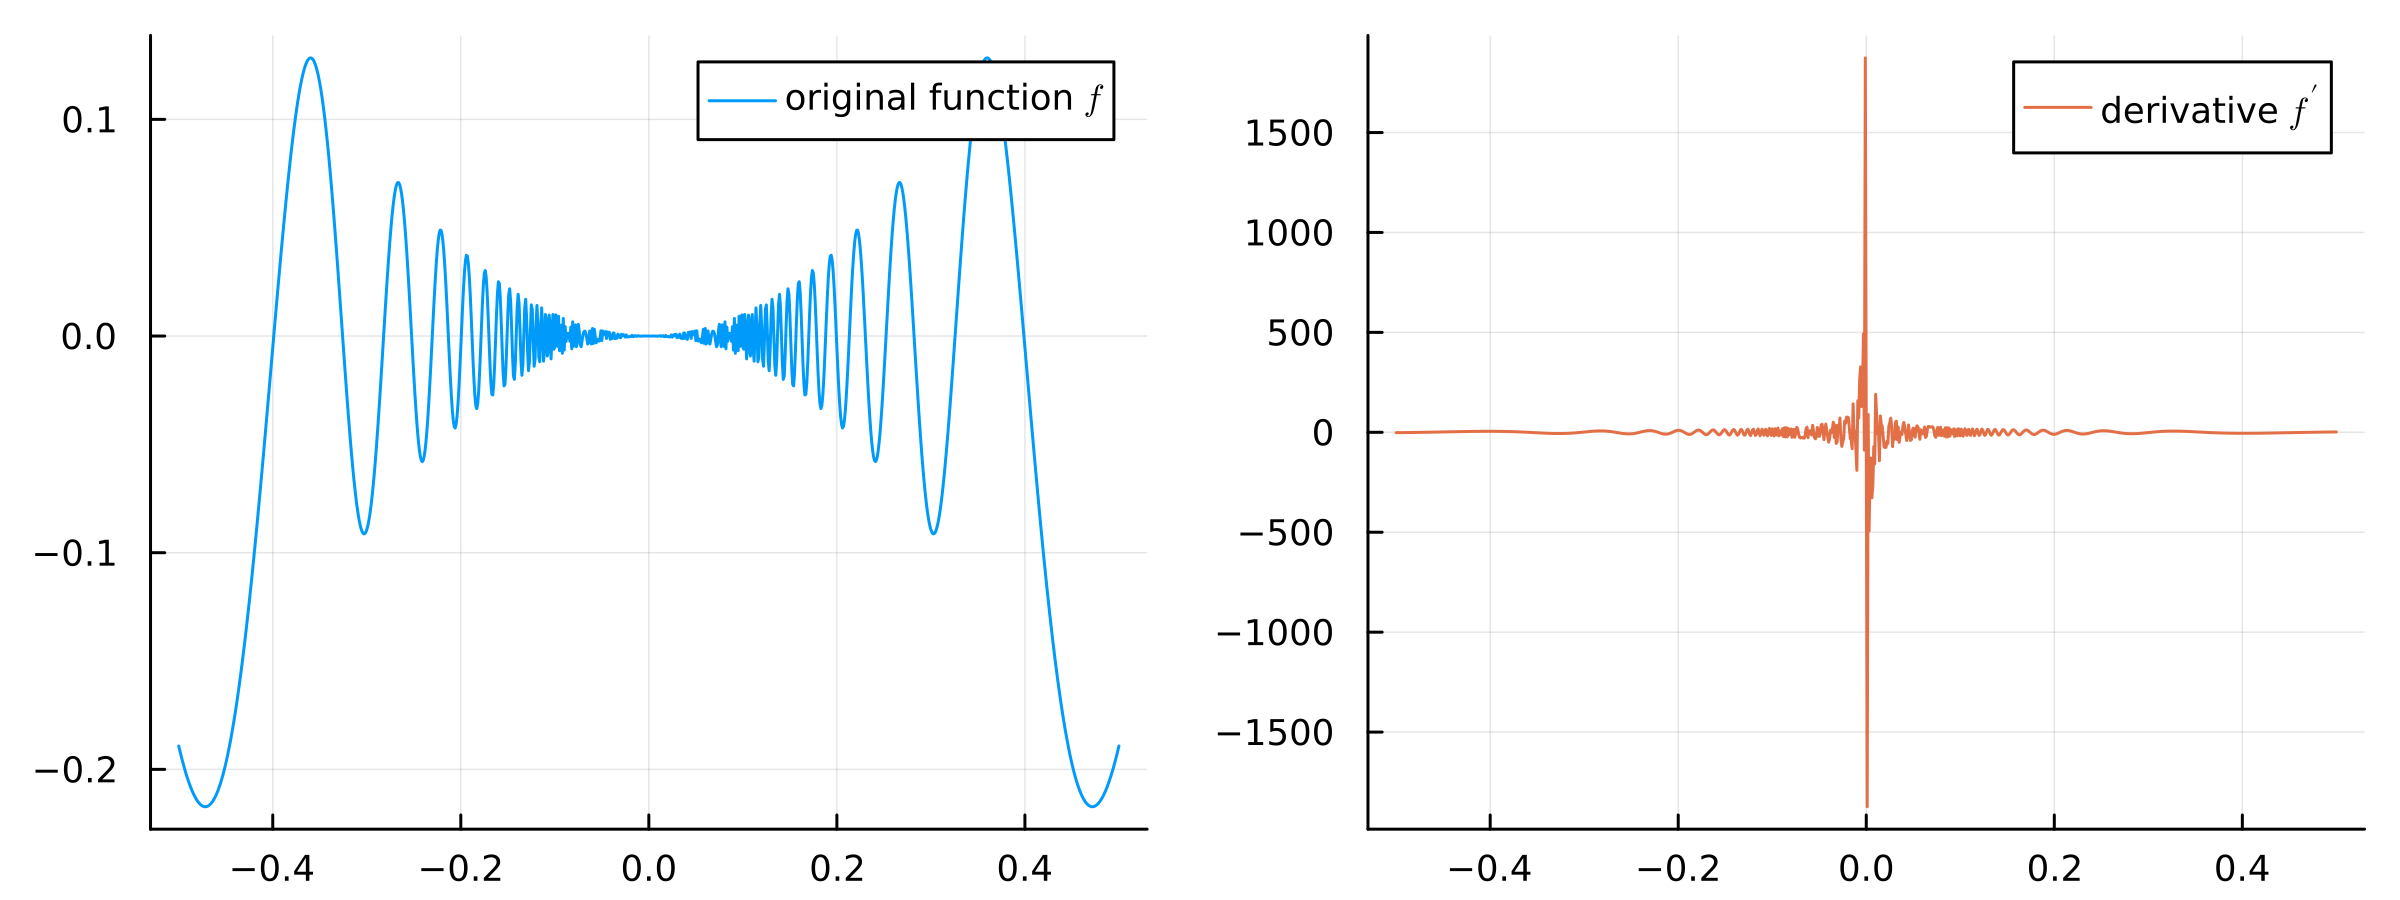
\includegraphics[scale=0.2]{figures/graph-004.png}
    \caption{Left: original function. Right: derivative.}
    \label{fig:4}
\end{figure}

\noindent Note that the derivative $f^\prime$ is not continuous at $x = 0$ since the limit of $f^\prime(x)$ does not exist as $x \to 0$. This example shows that the derivative of a function may not be continuous, and hence theorems for continuous functions do not apply to derivatives in general. However, the \textbf{intermediate value theorem}\index{intermediate value theorem for derivatives} is an exception. The intermediate value theorem for derivatives is also known as the \textbf{Darboux's theorem}\index{Darboux's theorem}.

\begin{theorem}[Darboux] \label{thm:12}
    Suppose $f$ is defined on $[a, b]$, and it has a derivative (finite or infinite) at each point in $(a, b)$. Assume also that the one-sided derivatives $f^\prime_{+}(a)$ and $f^\prime_{-}(b)$ both exist as finite numbers, and $f^\prime_{+}(a) \neq f^\prime_{-}(b)$. If $k$ is a number in between $f^\prime_{+}(a)$ and $f^\prime_{-}(b)$, then there exists an interior point $c \in (a, b)$ such that 
    \begin{align*}
        f^\prime(c) = k
    \end{align*}
\end{theorem}

\begin{proof}
    Note that $f$ is continuous on the entire closed interval $[a, b]$.

    \par We first consider the case where $k = [f(b) - f(a)] / (b-a)$. Then by applying the mean value theorem (Theorem~\ref{thm:8}), there exists $c \in (a, b)$ such that $f^\prime(c) = [f(b) - f(a)] / (b-a) = k$.

    \par Now, we suppose $k \neq [f(b) - f(a)] / (b-a)$. We note that either $f^\prime_{+}(a) \neq [f(b) - f(a)] / (b-a)$ or $f^\prime_{-}(b) \neq [f(b) - f(a)] / (b-a)$ since $f^\prime_{+}(a) \neq f^\prime_{-}(b)$. In other words, $k$ is either in between $f^\prime_{+}(a)$ and $[f(b) - f(a)] / (b-a)$ to it is in between $f^\prime_{-}(b)$ and $[f(b) - f(a)] / (b-a)$.

    \par Without loss of generality, we may assume $k$ is in between $f^\prime_{+}(a)$ and $[f(b) - f(a)] / (b-a)$. Define a function $\phi$ on $[a, b]$ by
    \begin{align*}
        \phi(x) = \begin{cases}
            \frac{f(x) - f(a)}{x - a}
            &x \neq a \\ 
            f^\prime_{+}(a)
            &x = a
        \end{cases}
    \end{align*}
    Note that $\phi$ is continuous on $[a, b]$, and $k$ is in between $\phi(a)$ and $\phi(b)$. Hence, we may apply the intermediate values theorem for continuous functions (Theorem~\ref{thm:11}) to $\phi$, there is a number $d \in (a, b)$ such that 
    \begin{align*}
        k = \phi(d) = \frac{f(d) - f(a)}{d - a}
    \end{align*}
    Then applying the mean value theorem (Theorem~\ref{thm:8}) to the fraction on the right-hand side of the above equation, we have 
    \begin{align*}
        k = \frac{f(d) - f(a)}{d - a}
        = f^\prime(c)
    \end{align*}
    for some $c$ in between $a$ and $d$.

    \par For the case where $k$ lying in between $f^\prime_{-}(b)$ and $[f(b) - f(a)] / (b-a)$, it can be proved with a similar argument, started by defining
    \begin{align*}
        \phi(x) = \begin{cases}
            \frac{f(x) - f(b)}{x - b}
            &x \neq b \\ 
            f^\prime_{-}(b)
            &x = b
        \end{cases}
    \end{align*}
\end{proof}

\par Essentially, Darboux's theorem tells us that though the derivative may not be continuous, it cannot have any \textit{jump discontinuities}. The following is another classical example in addition to the one in Exercise~\ref{ex:1}.

\begin{example}
    Consider the function 
    \begin{align*}
        f(x) = x^2 \sin\frac{1}{x} \ind\{x \neq 0\}
        = \begin{cases}
            x^2 \sin\frac{1}{x}
            &x \neq 0 \\ 
            0 & x = 0
        \end{cases}
    \end{align*}
    Its derivative is given by 
    \begin{align*}
        f^\prime(x)
        = \begin{cases}
            2x \sin\frac{1}{x} - \cos\frac{1}{x}
            &x \neq 0 \\ 
            0 & x = 0
        \end{cases}
    \end{align*}
    Note that the derivative $f^\prime$ is not continuous at $x = 0$. The graphs of $f$ and $f^\prime$ are shown in Figure~\ref{fig:6}.
    \begin{figure}[ht]
        \centering
        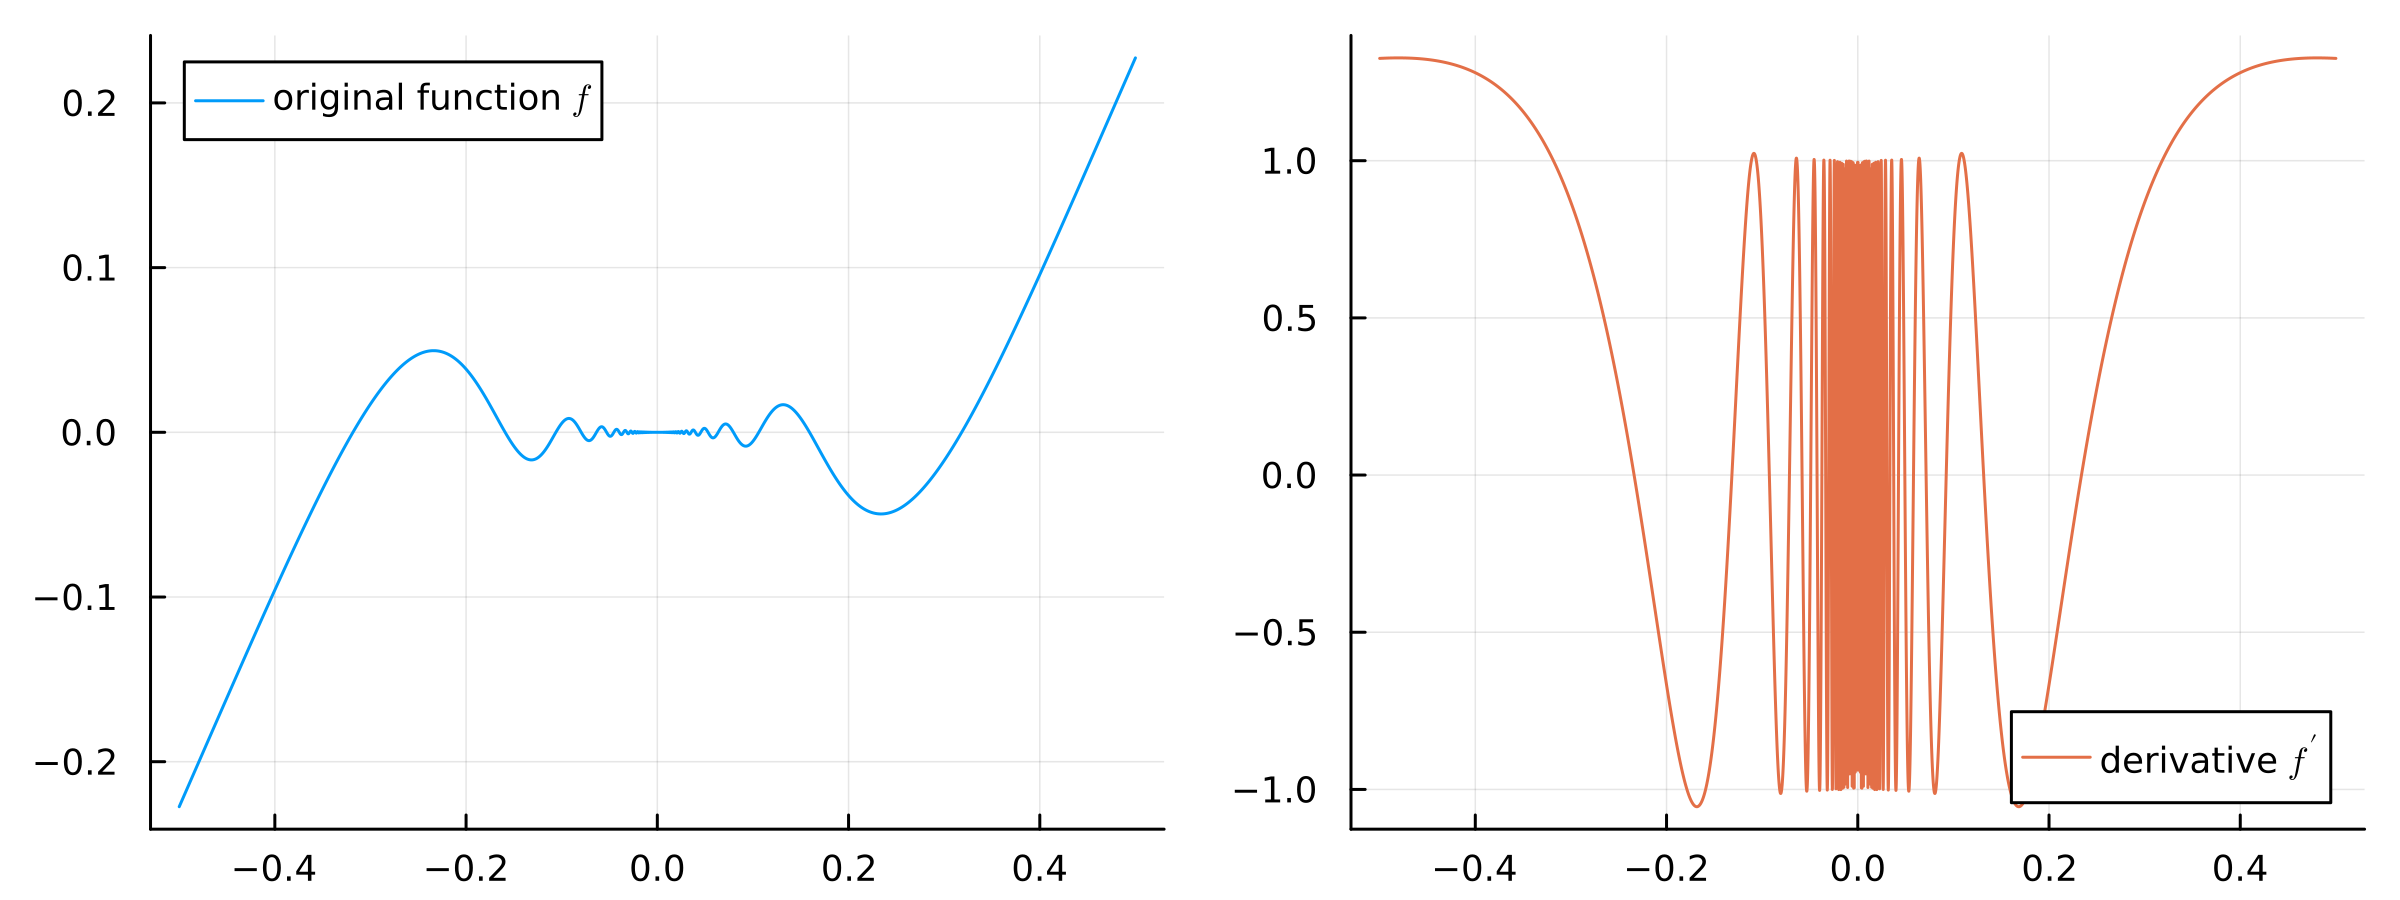
\includegraphics[scale=0.2]{figures/graph-007.png}
        \caption{Left: original function. Right: derivative.}
        \label{fig:6}
    \end{figure}
\end{example}

\par Actually, there is no need to require that $f^\prime_{+}(a)$ and $f^\prime_{-}(b)$ to be finite numbers in Theorem~\ref{thm:12}. The following theorem is an extension, and its proof is somewhat neater and more interesting than that of Theorem~\ref{thm:12}.

\begin{theorem} \label{thm:13}
    Suppose $f$ is defined on $[a, b]$, and it has a derivative (finite or infinite) at each point in $(a, b)$. Assume also that the one-sided derivatives $f^\prime_{+}(a)$ and $f^\prime_{-}(b)$ both exist (each of the two can either be finite or infinite), and $f^\prime_{+}(a) \neq f^\prime_{-}(b)$. If $k$ is a number in between $f^\prime_{+}(a)$ and $f^\prime_{-}(b)$, then there exists an interior point $c \in (a, b)$ such that 
    \begin{align*}
        f^\prime(c) = k
    \end{align*}
\end{theorem}

\begin{proof}
    Without loss of generality, we may assume $f^\prime_{+}(a) < k <  f^\prime_{-}(b)$. Define a function $g$ on $[a, b]$ by the equation
    \begin{align*}
        g(x) = f(x) - kx
    \end{align*}
    Note that $g$ is continuous on $[a, b]$, and the derivative of $g$ exists at each point in $(a, b)$. Furthermore, the one-sided derivatives of $g$, $g^\prime_{+}(a)$ and $g^\prime_{-}(b)$, both exist, which are given by
    \begin{align}
        g^\prime_{+}(a) = f^\prime_{+}(a) - k
        \quad \text{and} \quad 
        g^\prime_{-}(b) = f^\prime_{-}(b) - k
        \label{eq:17}
    \end{align} 
    It should be emphasized that \eqref{eq:17} also holds for infinite values. 

    \par Because we assume $f^\prime_{+}(a) < k <  f^\prime_{-}(b)$, \eqref{eq:17} yields
    \begin{align*}
        g^\prime_{+}(a) < 0
        \quad \text{and} \quad 
        g^\prime_{-}(b) > 0
    \end{align*} 
    It then follows from Theorem~\ref{thm:14} that there exist points $t_1$ and $t_2$ at which
    \begin{align*}
        g(t_1) < g(a)
        \quad \text{and} \quad 
        g(t_2) < g(b)
    \end{align*}
    This implies that $g$ must attain its minimum at some interior point $c \in (a, b)$ rather than at the endpoints. Then by applying Theorem~\ref{thm:5}, we have 
    \begin{align*}
        g^\prime(c) = 0
    \end{align*}
    Because $g^\prime(x) = f^\prime(x) - k \; \forall x \in (a, b)$, it follows that
    \begin{align*}
        f^\prime(c) = k
    \end{align*}
    This completes the proof.
\end{proof}

\begin{example}
    Consider a function defined on $[0, 1]$ given by 
    \begin{align*}
        f(x) = \sqrt[3]{x(x-1)},
        \quad x \in [0, 1]
    \end{align*}
    Note that the derivative exists as a finite number in $(0, 1)$. And it can be shown that $f^\prime_{+}(0) = -\infty$ and $f^\prime_{-}(1) = \infty$. Then Theorem~\ref{thm:13} tells us $f^\prime$ takes all the real numbers in $(0, 1)$. See Figure~\ref{fig:5}.
    \begin{figure}[ht]
        \centering
        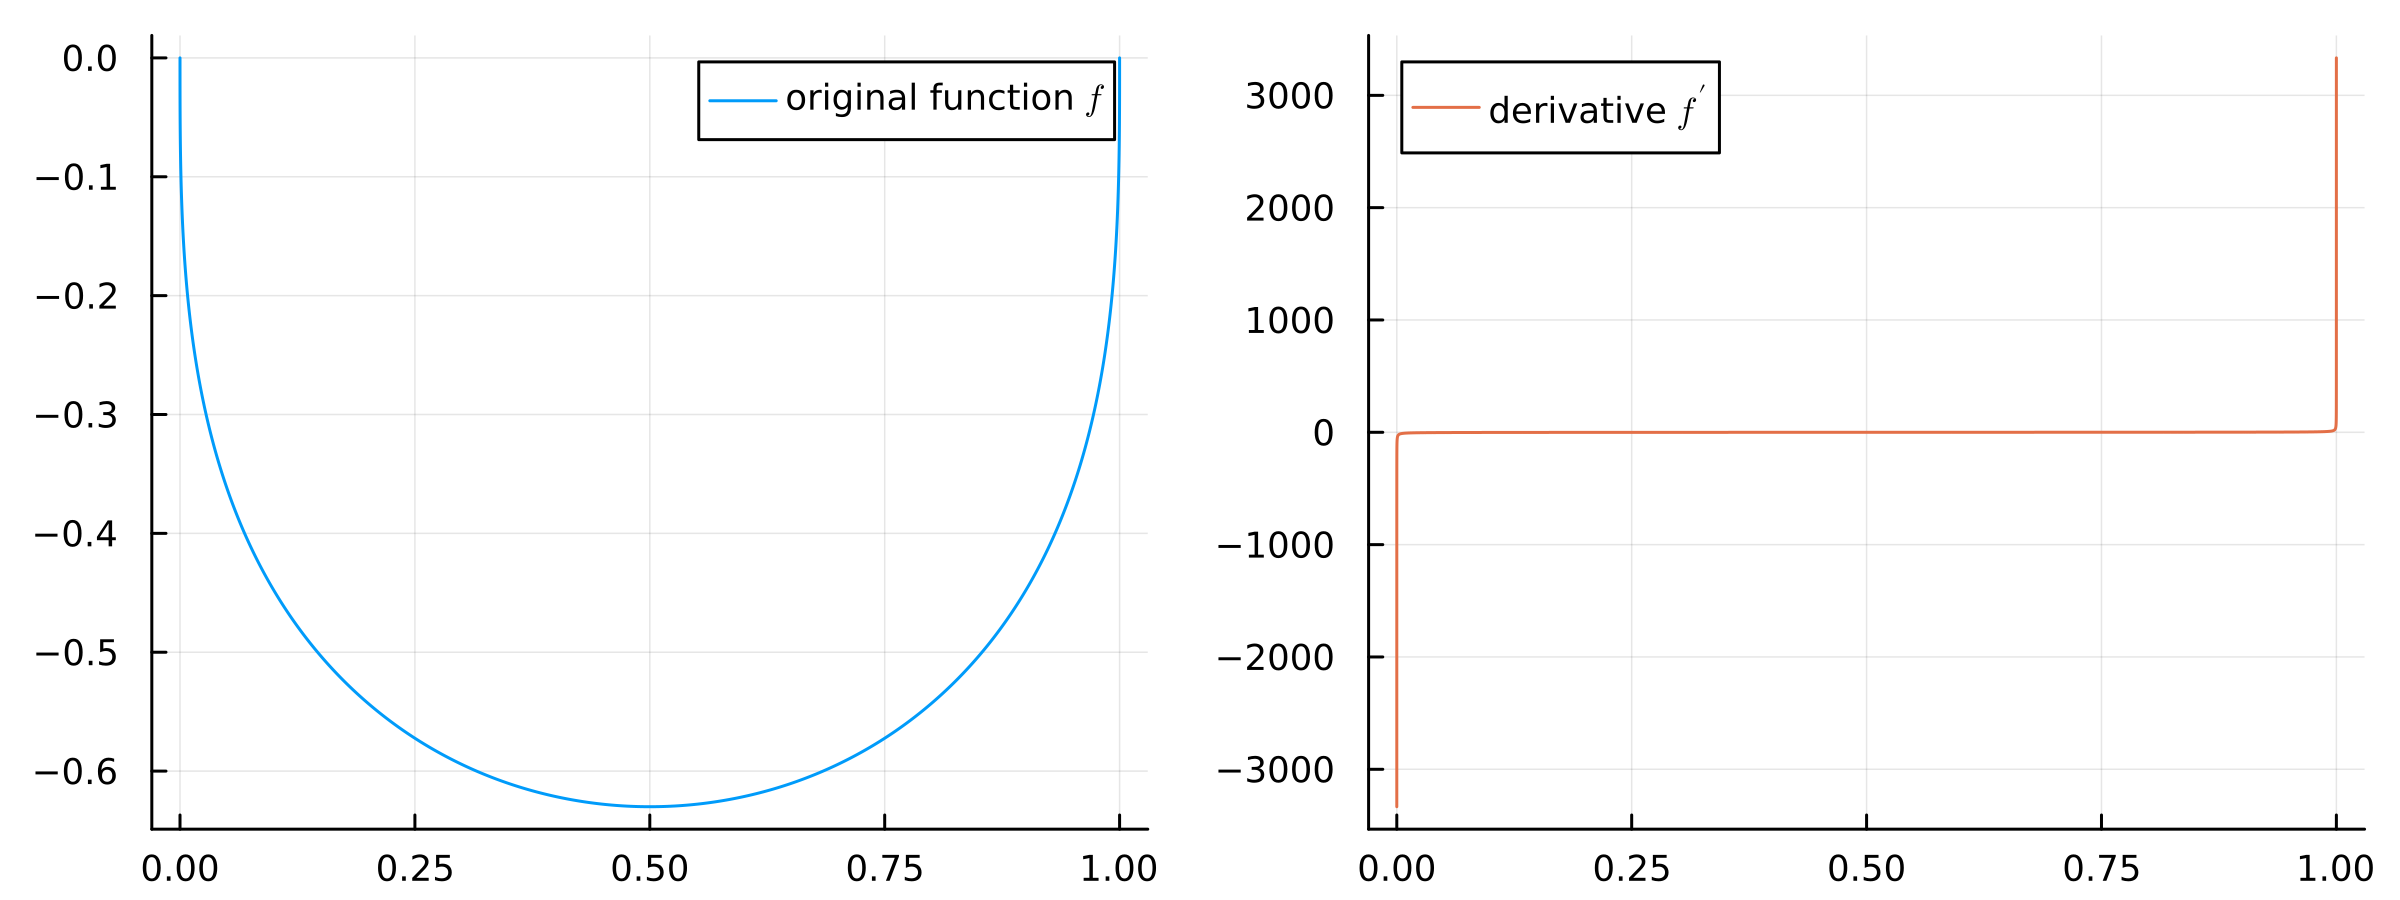
\includegraphics[scale=0.2]{figures/graph-006.png}
        \caption{Left: original function. Right: derivative.}
        \label{fig:5}
    \end{figure}

    \begin{note}
        Theoretically, the graph of $f^\prime$ in Figure~\ref{fig:5} will tend to $-\infty$ and $\infty$ as $x$ approaches $0$ and $1$, respectively. The reason why the absolute values of the derivatives near the endpoints shown in the graph are only about $3000$ is because of the limited computational precision of the computer.
    \end{note}
\end{example}

%------------------------------

\par By Theorem~\ref{thm:10}, we know a function is strictly increasing if its derivative is always positive, and it is strictly decreasing if its derivative is always negative. Suppose now we only know that $f^\prime$ is nonzero in some open interval, what can we conclude? Thanks to the intermediate value theorem, or Darboux's theorem, $f^\prime$ is either always positive or always negative. Hence, we can conclude that $f$ must be strictly monotonic. 

\begin{theorem}
    Suppose $f$ has a derivative (finite or infinite) in $(a, b)$, and is continuous at endpoints $a$ and $b$. If $f^\prime(x) \neq 0 \; \forall x \in (a, b)$, then $f$ is strictly monotonic on $[a, b]$.
\end{theorem}

\begin{proof}
    Pick a point $x_1 \in (a, b)$. Suppose $f^\prime(x_0) > 0$. Let $x_0$ be fixed, and choose an arbitrary point $x \in (a, b)$ other than $x_0$. We claim that $f^\prime(x) > 0$. Otherwise, if $f^\prime(x) < 0$, then by Theorem~\ref{thm:13}, there exists some point $c$ in between $x_0$ and $x$ such that $f^\prime(c) = 0$, which contradicts the given condition that $f^\prime$ is nonzero in $(a, b)$. In this case, we have $f^\prime(x) > 0 \; \forall x \in (a, b)$. It then follows from Theorem~\ref{thm:10} that $f$ is strictly increasing on $[a, b]$.

    \par If $f^\prime(x_0) < 0$, then a similar argument will show that $f$ is strictly decreasing on $[a, b]$.
\end{proof}

%------------------------------

\par It is because the derivatives cannot have jump discontinuities that monotonic derivatives are necessarily continuous.

\begin{theorem}
    Suppose $f^\prime$ exits, and is monotonic in $(a, b)$. Then $f^\prime$ is continuous in $(a, b)$.
\end{theorem}

\begin{proof}
    Without loss of generality, suppose that $f^\prime$ is increasing. We shall prove by contradiction. Assume that $f^\prime$ is discontinuous at $x = c \in (a, b)$. By Theorem~\ref{thm:15}, we have $f^\prime(c-)$ and $f^\prime(c+)$ both exist, and 
    \begin{align*}
        f^\prime(c-) \leq f(c) \leq f^\prime(c+)
    \end{align*}
    But because we assume $f^\prime$ is not continuous at $x = c$, it holds that 
    \begin{align*}
        f^\prime(c-) < f^\prime(c+)
    \end{align*}
    Let $[c-\delta, c+\delta]$ ($\delta > 0$) be a closed interval contained in $(a, b)$. We have 
    \begin{align*}
        f^\prime(c-\delta) \leq f^\prime(c-) < f^\prime(c+) \leq f^\prime(c+\delta)
    \end{align*}
    Let $k$ be a number in between $f^\prime(c-)$ and $ f^\prime(c+)$ other than $f^\prime(c)$. That is, 
    \begin{align*}
        f^\prime(c-) < k < f^\prime(c+) 
        \quad \text{and} \quad 
        k \neq f^\prime(c)
    \end{align*}
    
    \par Applying Theorem~\ref{thm:13} to $f^\prime$ on $[c-\delta, c+\delta]$, we conclude that there exists $x_0 \in (c-\delta, c+\delta)$ such that $f^\prime(x_0) = k$. But since $f^\prime$ is increasing, $f^\prime(c-) < k = f^\prime(x_0)$ and $k \neq f^\prime(c)$, we have $x_0 > c$. On the other hand, because $ f^\prime(x_0) = k < f^\prime(c+) $ and $k \neq f^\prime(c)$, we have $x_0 < c$. This leads to a contradiction. 
\end{proof}

%------------------------------

\section{Taylor's Theorem}

\par If $f$ is differentiable at $x = c$, then it can be approximated by 
\begin{align}
    f(x) \approx f(c) + f^\prime(c)(x-c)
    \label{eq:19}
\end{align}
when $\abs{x-c}$ is small. Geometrically, $f$ is close to its tangent line at $x=c$ near the point of tangency. Another way to look at \eqref{eq:19} is that $f$ is approximated by a polynomial of degree one whose first-order derivative at $x=c$ is exactly $f^\prime(c)$. And the value of this polynomial at $x=c$ is $f(c)$, that is, its zeroth-order derivative is $f(c)$. We can extend this idea by approximating $f$ with higher degree polynomials whose derivatives of all orders match with that of $f$ at $x = c$.

\begin{example}
    Suppose we know any order derivative of the function $f(x) = e^x$ is itself. That is,
    \begin{align*}
        f^{(k)}(x) = f(x) = e^x \quad \forall k = 0, 1, 2, \ldots
    \end{align*}
    Consider the polynomial 
    \begin{align*}
        p_n(x) 
        = \sum_{k=0}^n \frac{x^k}{k!}
        = 1 + x + \frac{x^2}{2} + \frac{x^3}{6} + \cdots + \frac{x^n}{n!}
    \end{align*}
    One can check that 
    \begin{align*}
        p^{(k)}_n(0) = f^{(k)}(0)
        \quad \forall k = 0, 1, \ldots, n
    \end{align*}
    Hence, it is reasonable to approximate $f(x)$ with $p_n(x)$ near point $x = 0$. Figure~\ref{fig:7} compares $f$ with $p_n$ with several choices of $n$.

    \begin{figure}[ht]
        \centering
        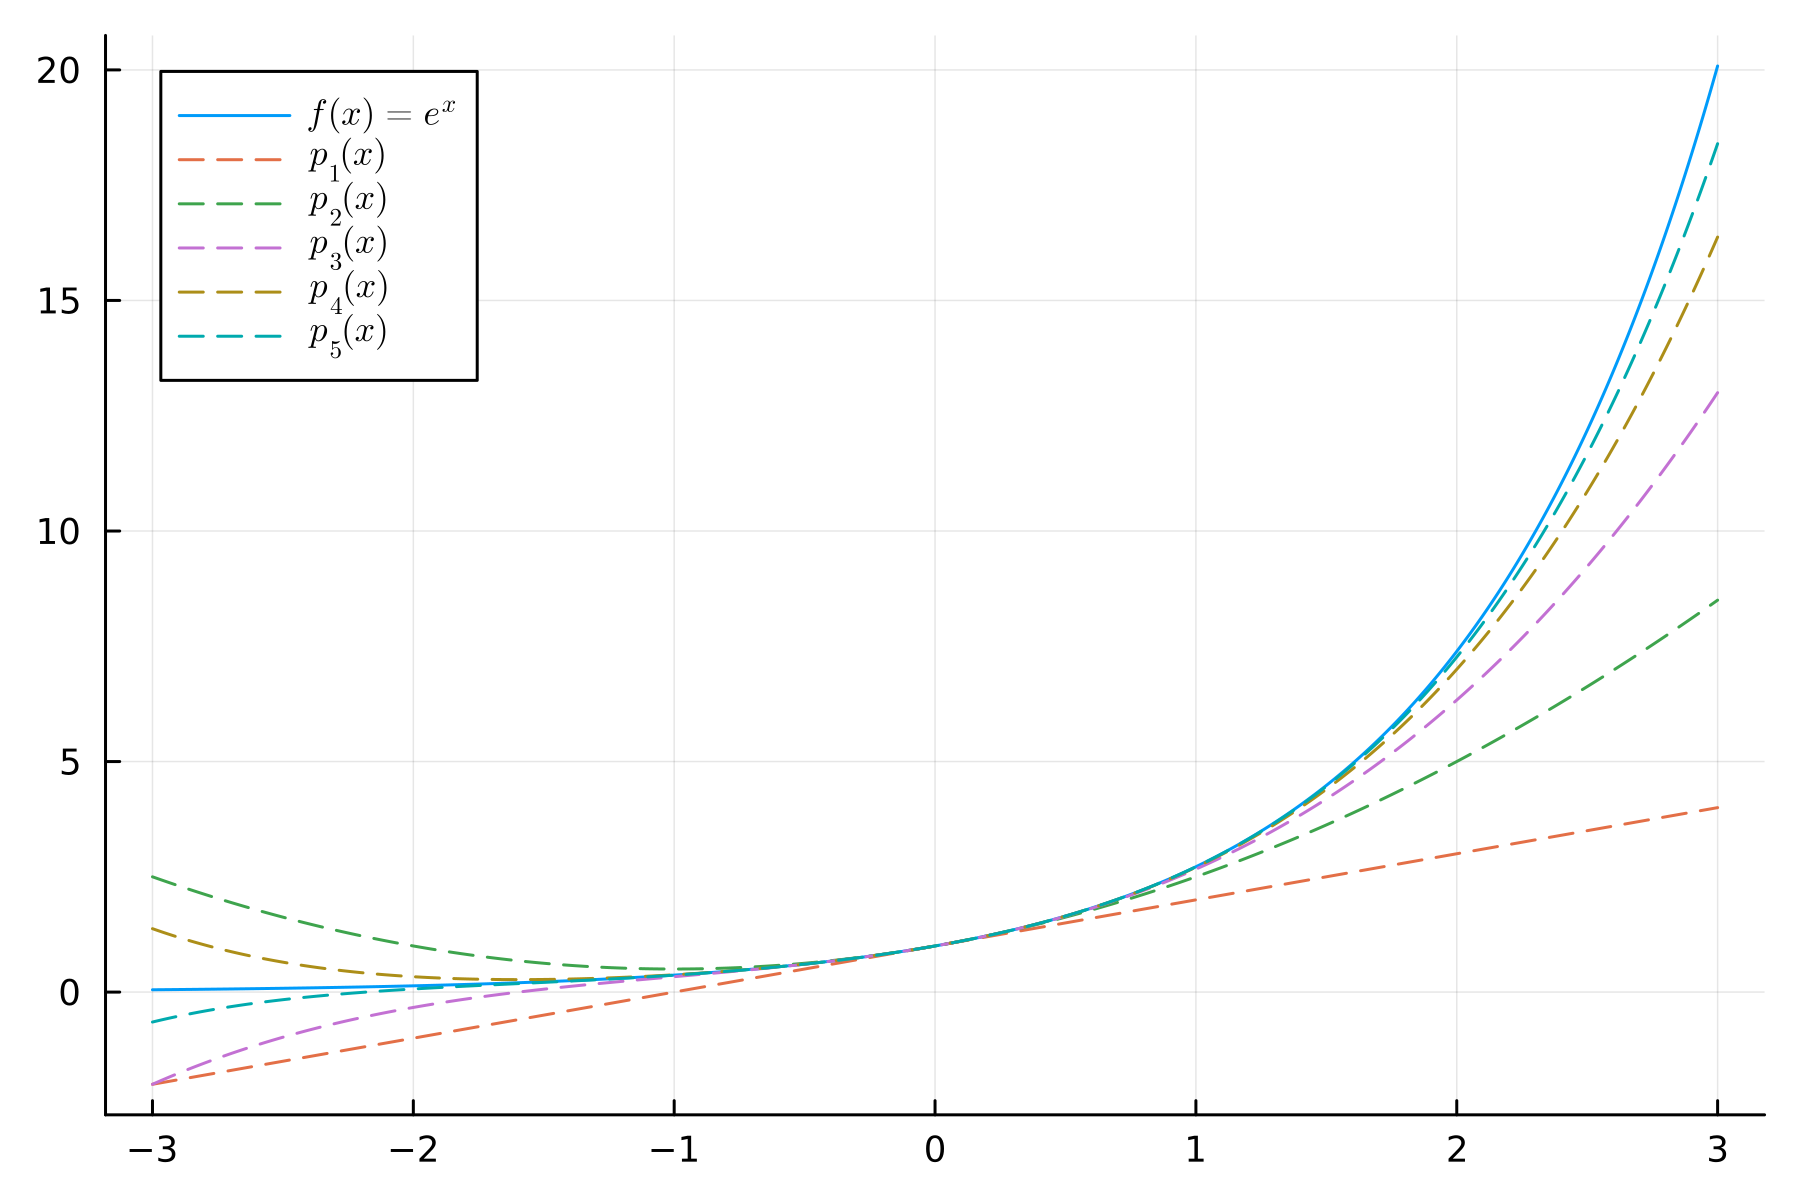
\includegraphics[scale=0.2]{figures/graph-008.png}
        \caption{Approximations of $f$ at $x=0$.}
        \label{fig:7}
    \end{figure}
\end{example}

%------------------------------

In general, a function $f$ can be approximated by the polynomial
\begin{align*}
    \sum_{k=0}^{n-1} \frac{f^{(k)}(c)}{k}(x-c)^k
    = f(c) + f^\prime(c)(x-c) + \cdots + \frac{f^{(n)}(c)}{n!} (x-c)^{n}
\end{align*}
at point $c$ provided that $f$ has up to $(n+1)$-th order derivative. The reason why we approximate $f$ with a polynomial of $n$ degree is that we have a remainder term, which makes use of the $(n+1)$-th order derivative. The remainder tells us how accurate the approximation is. The formal statement is described in the following theorem, the \textbf{Taylor's theorem}\index{Taylor's theorem}.

\begin{theorem}[Taylor] \label{thm:16}
    Let $f$ be a function having $(n+1)$-th order derivative everywhere in $(a, b)$, and suppose $f^{(n)}$ is continuous on $[a, b]$. Let $c \in (a, b)$ be an interior point. Then for every $x \in [a, b]$ other than $c$, we have 
    \begin{align}
        f(x) = \sum_{k=0}^{n} \frac{f^{(k)}(c)}{k!}(x-c)^k + \frac{f^{(n+1)}(\xi)}{(n+1)!} (x-c)^{n+1}
        \label{eq:20}
    \end{align}
    where $\xi$ is some number in between $x$ and $c$.
\end{theorem}

\par This theorem can be obtained as an immediate corollary of the following extension of the mean value theorem.

\begin{theorem} \label{thm:17}
    Let $f$ and $g$ be two functions each having $(n+1)$-th order derivative everywhere in $(a, b)$. Suppose that $f^{(n)}$ and $g^{(n)}$ are both continuous on $[a, b]$. Let $c \in (a, b)$ be an interior point. Then for every $x \in [a, b]$ other than $c$, we have 
    \begin{align}
        \left[
            f(x) - \sum_{k=0}^{n} \frac{f^{(k)}(c)}{k!}(x-c)^k
        \right] g^{(n+1)}(\xi)
        = f^{(n+1)}(\xi) \left[
            g(x) - \sum_{k=0}^{n} \frac{g^{(k)}(c)}{k!}(x-c)^k
        \right] 
        \label{eq:21}
    \end{align}
    where $\xi$ is some number in between $x$ and $c$.
\end{theorem}

\begin{remark}
    Taking $g(x) = (x-c)^{n+1}$, we have
    \begin{align*}
        g^{(n+1)}(\xi) = (n+1)!
        \quad \text{and} \quad
        \sum_{k=0}^{n} \frac{g^{(k)}(c)}{k!}(x-c)^k = 0
    \end{align*}
    Then \eqref{eq:21} reduces to \eqref{eq:20}, and hence this theorem reduces to Theorem~\ref{thm:16}.
\end{remark}

\begin{proof}
    Define functions $F(t)$ and $G(t)$ on $[a, b]$ by 
    \begin{align*}
        F(t) = \sum_{k=0}^{n} \frac{f^{(k)}(t)}{k!}(x-t)^k
        \quad \text{and} \quad 
        G(t) = \sum_{k=0}^{n} \frac{g^{(k)}(t)}{k!}(x-t)^k
        \quad \forall t \in [a, b]
    \end{align*}
    Note that $F$ and $G$ are continuous on $[a, b]$, and they have derivatives everywhere in $(a, b)$. Applying the generalized mean value theorem (Theorem~\ref{thm:7}) to $F(t)$ and $G(t)$ on the closed interval joining points $x$ and $c$, we have 
    \begin{align}
        [F(x) - F(c)] G^\prime(\xi)
        = F^\prime(\xi) [G(x) - G(c)]
        \label{eq:22}
    \end{align}
    for some number $\xi$ in between $x$ and $c$.

    \par After a few steps of computation, we obtain derivatives $F^\prime(t)$ and $G^\prime(t)$ as follows.
    \begin{align}
        F^\prime(t) = \frac{f^{(n+1)}(t)}{n!}(x-t)^{n}
        \quad \text{and} \quad 
        G^\prime(t) = \frac{g^{(n+1)}(t)}{n!}(x-t)^{n}
        \quad \forall t \in (a, b)
        \label{eq:23}
    \end{align}
    We also note that 
    \begin{align}
        F(x) = f(x), 
        \quad
        F(c) = \sum_{k=0}^{n} \frac{f^{(k)}(c)}{k!}(x-c)^k, 
        \quad
        G(x) = g(x), 
        \quad \text{and} \quad
        G(c) = \sum_{k=0}^{n} \frac{g^{(k)}(c)}{k!}(x-c)^k
        \label{eq:24}
    \end{align}
    Plugging \eqref{eq:23} and \eqref{eq:24} into \eqref{eq:22} leads to \eqref{eq:21}.
\end{proof}

\par We can rewrite \eqref{eq:20} as 
\begin{align*}
    f(x) = p_n(x) + r_n(x)
\end{align*}
where 
\begin{align*}
    p_n(x) = \sum_{k=0}^{n} \frac{f^{(k)}(c)}{k!}(x-c)^k
\end{align*}
is the polynomial approximation, and 
\begin{align*}
    r_n(x) = \frac{f^{(n+1)}(\xi)}{(n+1)!} (x-c)^{n+1}
\end{align*}
is the remainder. The smaller the absolute value of $r_n(x)$ is, the more accurate the approximation will be.


\begin{exercise}
    Use Taylor's theorem (Theorem~\ref{thm:16}) to approximate the value of $\ln(0.6)$ so that the absolute error is less than $0.1$.
\end{exercise}

\begin{solution}
    Putting $f(x) = \ln(x)$ in \eqref{eq:20}, we have
    \begin{align*}
        p_n(x;c) &= \sum_{k=0}^{n} \frac{f^{(k)}(c)}{k!}(x-c)^k
        = \ln(c) + \sum_{k=1}^{n} \frac{(-1)^{k+1}}{k c^n}(x-c)^k \\ 
        r_n(x;c) &= \frac{(-1)^{n+2}}{(n+1) \xi^{n+1}}(x-c)^{n+1}
    \end{align*}
    Since the value of $\ln(x)$ at $x=1$ is known, i.e., $\ln(1) = 0$, we can expand it about that point by putting $c=1$. Then we have 
    \begin{align*}
        p_n(x) = \sum_{k=1}^{n} \frac{(-1)^{k+1}}{k}(x-1)^k
        \quad \text{and} \quad
        r_n(x) = \frac{(-1)^{n+2}}{(n+1) \xi^{n+1}}(x-1)^{n+1}
    \end{align*}
    To approximate $\ln(0.6)$ by $p_n(0.6)$ within the error bounds, we need to estimate the remainder $r_n(0.6)$. Note that $\xi$ is now some number in between $0.6$ and $1$ since $x=0.6$ and $c=1$. The absolute value of $r_n(0.6)$ is bounded above by 
    \begin{align}
        \abs{r_n(0.6)} = \frac{1}{n+1} \abs{\frac{0.6-1}{\xi}}^{n+1}
        < \frac{1}{n+1} \left(\frac{0.4}{0.6}\right)^{n+1}
        = \frac{1}{n+1} \left(\frac{2}{3}\right)^{n+1}
        \label{eq:25}
    \end{align}


    \par We then estimate $\abs{r_n(0.6)}$ using \eqref{eq:25} by trying the first few values of $n$. We have 
    \begin{align*}
        r_1(0.6) = \frac{2}{9} > 0.1
        \quad \text{and} \quad 
        r_2(0.6) = \frac{8}{81} < 0.1
    \end{align*}
    Hence, it is adequate to approximate $\ln(0.6)$ by $p_2(0.6)$. The approximated value is
    \begin{align*}
        \ln(0.6) \approx p_2(0.6) = (0.6-1) - \frac{1}{2} \times (0.6-1)^2 = -0.48
    \end{align*}
    We can also visualize the result in Figure~\ref{fig:8}. As we can see, the approximated value is quite close to the true value. And the absolute error is actually much less than the required bound, $0.1$.
    \begin{figure}[ht]
        \centering
        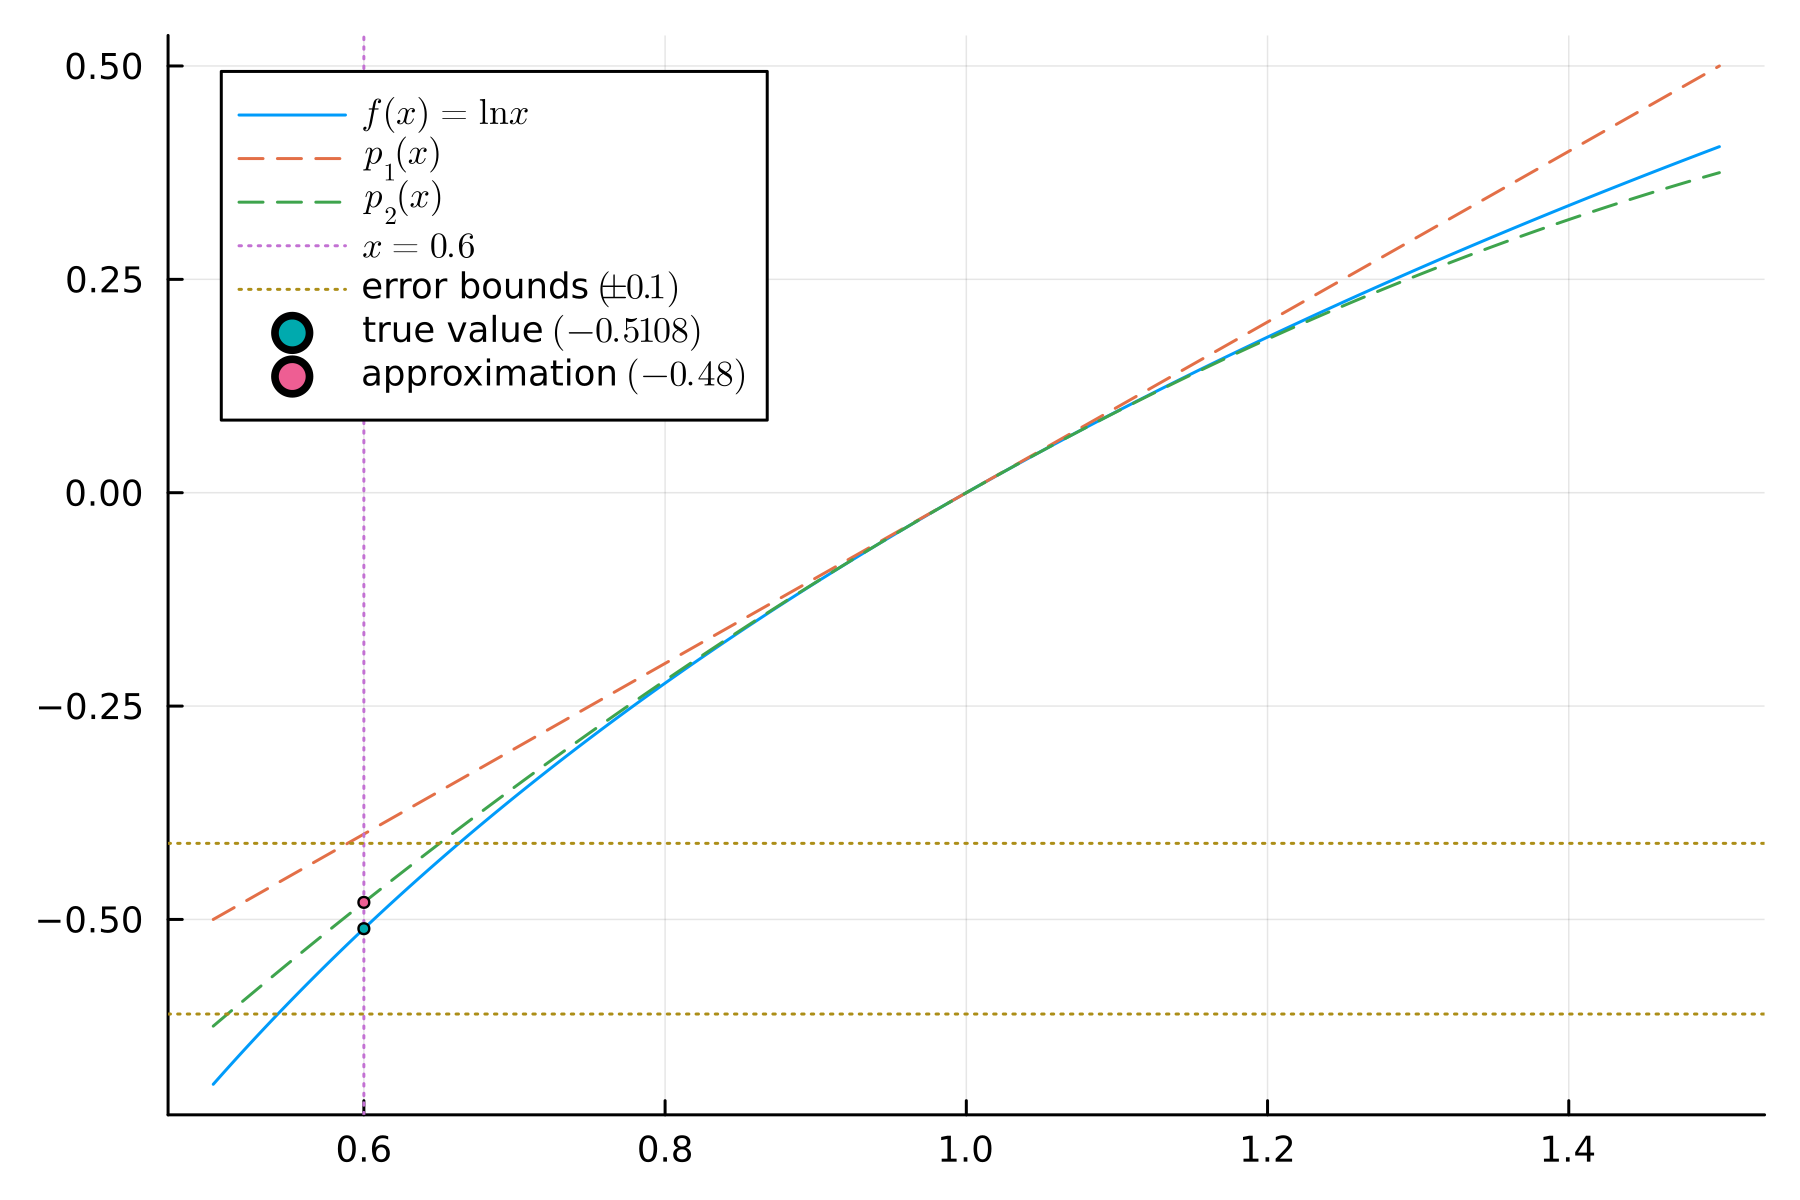
\includegraphics[scale=0.2]{figures/taylor-approx.png}
        \caption{Approximation of $\ln(0.6)$.}
        \label{fig:8}
    \end{figure}
\end{solution}

%==============================

\chapter{Functions of Bounded Variation}

%------------------------------

\section{Definition of Functions of Bounded Variation}

%------------------------------

\begin{definition}
    Let $f: [a, b] \to \R$ be a function. For a partition $P = \{ x_0, x_1, \ldots, x_n \}$ on $[a, b]$, write
    \begin{align*}
        V(P, f) := \sum_{k=1}^n \abs{\Delta f_k} = \sum_{k=1}^n \abs{f(x_k) - f(x_{k-1})}
    \end{align*}
    If there exists $M > 0$ such that
    \begin{align*}
        V(P, f) < M
    \end{align*}
    holds for all partition $P$, then we say $f$ is of bounded variation on $[a, b]$.
\end{definition}

%------------------------------

\begin{theorem} \label{thm:35}
    If $f$ is of bounded variation on $[a, b]$, then $f$ is bounded on $[a, b]$.
\end{theorem}

\begin{remark}
    The converse is not true. That is, if $f$ is a bounded function, then it may not be of bounded variation (see Example~\ref{eg:6}).
\end{remark}

\begin{proof}
    Pick any $x \in [a, b]$. Consider the partition $P = \left\{a, b\right\} \cup \left\{x\right\}$. Since $f$ is of bounded variation, we have 
    \begin{align*}
        \abs{\abs{f(x)} - \abs{f(a)}}
        \leq \abs{f(x) - f(a)}
        \leq V(P, f)
        < M
    \end{align*}
    where $M$ is a constant that is independent of $x$. It follows that 
    \begin{align*}
        \abs{f(x)} \leq \abs{f(a)} + M
        \quad \forall x \in [a, b]
    \end{align*}
    Therefore, $f$ is bounded on $[a, b]$.
\end{proof}

\begin{example}
    Let $f: [0, 1] \to \R$ be given by 
    \begin{align*}
        f(x) = \begin{cases}
            x\cos \frac{\pi}{x} &0 < x \leq 1 \\
            0 &x = 0
        \end{cases}
    \end{align*}
    Note that $f$ is a bounded continuous function on $[0, 1]$. We now show that $f$ is however not of bounded variation. Consider a sequence of partitions 
    \begin{align*}
        P_1 &= \left\{
            0, \frac{1}{3}, \frac{1}{2}, 1
        \right\} \\ 
        P_2 &= \left\{
            0, 
            \frac{1}{5}, \frac{1}{4},
            \frac{1}{3}, \frac{1}{2}, 
            1
        \right\} \\ 
        P_3 &= \left\{
            0, 
            \frac{1}{7}, \frac{1}{6},
            \frac{1}{5}, \frac{1}{4},
            \frac{1}{3}, \frac{1}{2}, 
            1
        \right\} \\ 
        &\vdots \\ 
        P_n &= \left\{
            0, 1
        \right\} \cup \bigcup_{k=1}^n \left\{
            \frac{1}{2k+1}, \frac{1}{2k}
        \right\} \\ 
        &\vdots
    \end{align*}
    For partition $P_n$, the sum 
    \begin{align*}
        V(P, f)
        &> \sum_{k=1}^n \abs{
            f\left( \frac{1}{2k} \right) 
            - f\left( \frac{1}{2k+1} \right)
        } \\
        &= \sum_{k=1}^n \abs{
            \frac{1}{2k}\cos(2k\pi) 
            - \frac{1}{2k+1}\cos((2k+1)\pi)
        } \\ 
        &= \sum_{k=1}^n (
            \frac{1}{2k}
            + \frac{1}{2k+1}
        ) \\ 
        &= \sum_{k=2}^{2n+1} \frac{1}{k}
    \end{align*}
    Since the series $\sum \frac{1}{k} = \infty$, we can always find a partition such that the sum $\sum \abs{\Delta f_k}$ exceeds any given positive number. Therefore, $f$ is not of bounded variation on $[0, 1]$ though it is bounded.
    \label{eg:6}
\end{example}

\par Recall the definition of uniform continuity. The condition of uniform continuity, to some extent, eliminates the functions that tend to infinity at some points while the condition of bounded variation eliminates the functions that \textit{oscillate}. 

%------------------------------

\begin{theorem} \label{thm:36}
    If $f$ is a monotonic function on $[a, b]$, then $f$ is of bounded variation on $[a, b]$.
\end{theorem}

\begin{proof}
    Without loss of generality, we assume $f$ is increasing. For any partition $P = \left\{x_0, \ldots, x_n\right\}$ on $[a, b]$, we have 
    \begin{align*}
        \sum_{k=1}^n \abs{\Delta f_k}
        = \sum_{k=1}^n \abs{f(x_k) - f(x_{k-1})}
        = \sum_{k=1}^n f(x_k) - f(x_{k-1})
        = f(b) - f(a)
    \end{align*}
    This completes the proof since $f(b) - f(a)$ is independent of $P$.
\end{proof}

%------------------------------

\section{Total Variation}

%------------------------------

\begin{definition}
    Let $f$ be of bounded variation on $[a, b]$. The total variation of $f$ on $[a, b]$ is defined by 
    \begin{align*}
        V_a^b (f) 
        := \sup_{P \in \mathcal{P}[a, b]} V(P, f) 
    \end{align*}
    where $\mathcal{P}[a, b]$ is the collection of all partitions on $[a, b]$.
\end{definition}

\begin{note}
    We will sometimes write $V(f)$ instead of $V_a^b (f)$ to ease the notation if it does not confuse.
\end{note}

%------------------------------

\begin{theorem} \label{thm:33}
    If $f$ and $g$ are each of bounded variation on $[a, b]$, then $f \pm g$ and $f g$ are also of bounded variation. Moreover, 
    \begin{align}
        V(f \pm g) \leq V(f) + V(g) 
        \label{eq:77}
    \end{align}
    and 
    \begin{align}
        V(f g) &\leq \sup_{x\in [a, b]} \abs{g(x)} V(f) + \sup_{x \in [a, b]} \abs{f(x)} V(g)
        \label{eq:78}
    \end{align}
\end{theorem}

\begin{proof}
    (Proof of $f \pm g$ being of bounded variation) We have 
    \begin{align*}
        V(P, f \pm g)
        &= \sum_{k=1}^n \abs{(f \pm g)(x_k) - (f \pm g)(x_{k-1})} \\ 
        &= \sum_{k=1}^n \abs{( f(x_k) - f(x_{k-1}) ) \pm ( g(x_k) - g(x_{k-1}) )} \\ 
        &\leq \sum_{k=1}^n \abs{\Delta f_k} + \abs{\Delta g_k} \\ 
        &= V(P, f) + V(P, g) \\ 
        &\leq V(f) + V(g)
    \end{align*}
    Since $f$ and $g$ are both of bounded variation, $V(f), V(g) < \infty$. Therefore, $V(P, f \pm g)$ is bounded above by a finite number for any partition $P$, which implies the function $f \pm g$ is of bounded variation. Taking supremum over all $P$'s on 
    \begin{align*}
        V(P, f \pm g) \leq V(f) + V(g)
    \end{align*}
    we obtain \eqref{eq:77}.
    
    \par (Proof of $f g$ being of bounded variation) For any partition $P$ on $[a, b]$, we have 
    \begin{align*}
        V(P, f g)
        &= \sum_{k=1}^n \abs{f(x_k) g(x_k) - f(x_{k-1}) g(x_{k-1})} \\ 
        &= \sum_{k=1}^n \abs{
            f(x_k) g(x_k) 
            - f(x_{k-1}) g(x_k) 
            + f(x_{k-1}) g(x_k) 
            - f(x_{k-1}) g(x_{k-1})
        } \\  
        &= \sum_{k=1}^n \abs{
            g(x_k) \Delta f_k
            + f(x_{k-1}) \Delta g_k
        } \\ 
        &\leq \sup\abs{g} V(P, f) + \sup\abs{f} V(P, g) \\ 
        &\leq \sup\abs{g} V(f) + \sup\abs{f} V(g)
    \end{align*}
    Similarly, because $f$ and $g$ are of bounded variation, $V(f)$ and $V(g)$ are finite. Moreover, by Theorem~\ref{thm:35}, $f$ and $g$ are bounded on $[a, b]$, which implies $\sup\abs{f}, \sup\abs{g} < \infty$. Hence, $V(P, f g)$ is bounded above by a finite number for any partition, which implies $fg$ is also of bounded variation, and \eqref{eq:78} holds.
\end{proof}

%------------------------------

\section{Additive Property of Total Variation}

%------------------------------

\begin{theorem} \label{thm:34}
    Let $f$ be of bounded variation on $[a, b]$. For a point $c \in (a, b)$, we have $f$ is of bounded variation on $[a, c]$ and $[c, b]$, and 
    \begin{align}
        V_a^b(f) = V_a^c(f) + V_c^b(f)
        \label{eq:79}
    \end{align}
\end{theorem}

\begin{proof}
    Let $P^\prime$ be a partition on $[a, c]$ and $P^{\prime\prime}$ a partition on $[c, b]$. Note that $P = P^\prime \cup P^{\prime\prime}$ forms a partition on $[a, b]$. We have
    \begin{align*}
        V_a^b(P, f) = V_a^c(P^\prime, f) + V_c^b(P^{\prime\prime}, f)
    \end{align*}
    Since $f$ is of bounded variation on $[a, b]$, it follows that 
    \begin{align}
        \infty > V_a^b(f) 
        \geq V_a^b(P, f) 
        = V_a^c(P^\prime, f) + V_c^b(P^{\prime\prime}, f)
        \label{eq:80}
    \end{align}
    Note that \eqref{eq:80} holds for any partition $P^\prime$ on $[a, c]$ and any partition $P^{\prime\prime}$ on $[c, b]$. Therefore, $f$ is of bounded variation on $[a, c]$ and $[c, b]$, i.e., $V_a^c(f), V_c^b(f) < \infty$.

    Taking the supremum over all partitions on $[a, c]$ followed by taking the supremum over all partitions on $[a, c]$ on \eqref{eq:80}, we obtain
    \begin{align}
        V_a^b(f) 
        \geq \sup_{P^\prime \in \mathcal{P}[a, c]} V_a^c(P^\prime, f) 
        + \sup_{P^{\prime\prime} \in \mathcal{P}[c, b]} V_c^b(P^{\prime\prime}, f)
        = V_a^c(f) + V_c^b(f)
        \label{eq:81}
    \end{align}

    \par Now, let $P$ be a partition on $[a, b]$. Let
    \begin{align*}
        P^\prime &= (P \cap [a, c]) \cup \{ c \} & 
        P^{\prime\prime} &= P \cap [c, b] \cup \{ c \}
    \end{align*}
    There are two cases. If $c \in P$, then
    \begin{align*}
        V_a^b(P, f) 
        = V_a^c(P^\prime, f) + V_c^b(P^{\prime\prime}, f)
    \end{align*}
    If $c \notin P$, then 
    \begin{align*}
        V_a^b(P, f) 
        \leq V_a^c(P^\prime, f) + V_c^b(P^{\prime\prime}, f)
    \end{align*}
    Either way, it holds that 
    \begin{align}
        V_a^b(P, f) 
        \leq V_a^c(P^\prime, f) + V_c^b(P^{\prime\prime}, f)
        \leq V_a^c(f) + V_c^b(f)
        \label{eq:82}
    \end{align}
    Taking the supremum over all partitions on $[a, b]$ on \eqref{eq:82}, we have 
    \begin{align}
        V_a^b(f)
        = \sup_{P \in \mathcal{P}[a, b]} V_a^b(P, f) 
        \leq V_a^c(f) + V_c^b(f)
        \label{eq:83}
    \end{align}

    Equation \eqref{eq:79} then follows from \eqref{eq:80} and \eqref{eq:83}.
\end{proof}

The total variation of a function with the same lower and upper limits is defined as zero, i.e., $V_x^x(f) = 0$ so that \eqref{eq:79} holds for $c = a$ and $c = b$.

\begin{definition} \label{def:3}
    Suppose that $f$ is of bounded variation on $[a, b]$. The total variation
    \begin{align*}
        V_a^x(f) \quad a \leq x \leq b
    \end{align*}
    can be regarded as a function of $x$ on $[a, b]$ with an addition definition $V_a^a(f) := 0$.
\end{definition}

%------------------------------

\section{Characterization of Functions of Bounded Variation}

In fact, all functions of bounded variation can be written as a difference between two increasing functions.

%------------------------------

\begin{lemma} \label{lem:2}
    Let $f$ be of bounded variation on $[a, b]$. Define $V(x) := V_a^x(f)$ ($a \leq x \leq b$). Then 
    \begin{enumerate}
        \item $V$ is increasing on $[a, b]$
        \item $V-f$ is increasing on $[a, b]$
    \end{enumerate}
\end{lemma}

\begin{proof}
    (Proof of 1) By Theorem~\ref{thm:34} and Definition~\ref{def:3}, we know $V(x)$ is well-defined, and 
    \begin{align*}
        V(x+h) - V(x) = V_x^{x+h}(f) \geq 0
    \end{align*}
    where $h > 0$. Therefore, $V$ is indeed increasing on $[a, b]$.

    (Proof of 2) Fix $x \in [a, b]$. Let $h$ be such that $0 \leq x < x+h \leq b$. Let a partition $P$ on $[x, x+h]$ be given by 
    \begin{align*}
        P = \{ x, x+h \}
    \end{align*}
    We have 
    \begin{align}
        V_x^{x+h}(P, f) = \abs{f(x+h) - f(x)} 
        \leq V_x^{x+h}(f)
        \label{eq:84}
    \end{align}
    It then follows from \eqref{eq:84} that 
    \begin{align*}
        (V-f)(x+h) - (V-f)(x)
        &= V_x^{x+h}(f) - (f(x+h) - f(x)) \\ 
        &\geq V_x^{x+h}(f) - \abs{f(x+h) - f(x)} \\ 
        &\geq 0
    \end{align*}
    Hence, $V-f$ is also an increasing function on $[a, b]$.
\end{proof}

%------------------------------

\begin{theorem}[Characterization of Functions of Bounded Variation] \label{thm:22}
    Let $f$ be a real-valued function on $[a, b]$. Then, the following statements are equivalent.
    \begin{enumerate}
        \item $f$ is of bounded variation on $[a, b]$.
        \item There exist two increasing functions $g$ and $h$ on $[a, b]$ such that $f = g - h$.
        \item There exist two \textbf{strictly} increasing functions $g$ and $h$ on $[a, b]$ such that $f = g - h$.
    \end{enumerate}
\end{theorem}

%==============================

\chapter{Riemann-Stieltjes Integral} \label{chap:1}

\section{Definition of the Riemann-Stieltjes Integral}

%------------------------------

\begin{definition} \label{def:1}
    Suppose that $f$ and $\alpha$ are \textbf{real-valued bounded} functions on $[a,b]$. Let $P = \left\{x_0, x_1, \ldots, x_n\right\}$ be a partition on $[a, b]$ and $t_k$ a point in the sub-interval $[x_{k-1}, x_k]$. A sum of the form 
    \begin{align*}
        S(P,f,\alpha)
        = \sum_{k=1}^n f(t_k) \Delta \alpha_k
    \end{align*}
    is called a Riemann-Stieltjes sum of $f$ with respect to $\alpha$. We say $f$ is Riemann-integrable with respect to $\alpha$, and write $f \in \mathfrak{R}(\alpha)$ on $[a,b]$ if there exists a number $A$ having the following property: for any given $\varepsilon > 0$, there exists a partition $P_\varepsilon$ such that 
    \begin{align*}
        \abs{S(P,f,\alpha) - A} < \varepsilon
    \end{align*}
    for any refinement $P$ of $P_\varepsilon$ and for any choice of points $t_k$. (Note that $S(P,f,\alpha)$ depends on $t_k$.) Moreover, the number $A$ is \textbf{uniquely} determined if it exists (this is proved in Proposition~\ref{pro:3}) and is denoted by \begin{align*}
        \int_a^b f \; \mathrm{d}\alpha
    \end{align*}
\end{definition}

\begin{note}
    To ease the nation, we will sometimes write
    \begin{align*}
        \sum_{k} f(t_k) \Delta \alpha_k
    \end{align*}
    without specifying the lower and upper limits of $k$ if no confusion will be caused.
\end{note}

%------------------------------

\par Recall Definition~\ref{def:1} only requires the existence of $A$. We now show that such number $A$ is also unique.

\begin{proposition} \label{pro:3}
    Let $S(P,f,\alpha)$ be as in Definition~\ref{def:1}. If $A$ and $A^\prime$ both satisfy the property stated in Definition~\ref{def:1}, then $A = A^\prime$.
\end{proposition}

\begin{proof}
    Given $\varepsilon > 0$, by the property in Definition~\ref{def:1}, there exist partitions $P_1$ and $P_2$ such that  
    \begin{align*}
        \abs{S(P_1,f,\alpha) - A} &< \varepsilon / 2 &
        \abs{S(P_2,f,\alpha) - A^\prime} &< \varepsilon / 2
    \end{align*}
    Let $P = P_1 \cup P_2$. We have
    \begin{align*}
        \abs{S(P,f,\alpha) - A} &< \varepsilon / 2 &
        \abs{S(P,f,\alpha) - A^\prime} &< \varepsilon / 2
    \end{align*}
    It then follows that
    \begin{align*}
        \abs{A - A^\prime}
        \leq \abs{S(P,f,\alpha) - A} +
        \abs{S(P,f,\alpha) - A^\prime} 
        < \varepsilon / 2 + \varepsilon / 2
        = \varepsilon
    \end{align*}
    Since $\varepsilon > 0$ is arbitrary, we must have $A = A^\prime$.
\end{proof}

%------------------------------

\section{Linear Properties}

%------------------------------

\par The integral is linear in the integrand. In other words, the integral of a linear combination of functions is equal to the linear combination of integrals of each function.

\begin{theorem} \label{thm:18}
    Suppose that $f, g \in \mathfrak{R}(\alpha)$ on $[a,b]$. Then $c_1 f + c_2 g \in \mathfrak{R}(\alpha)$ on $[a,b]$ where $c_1$ and $c_2$ are constants. In that case, 
    \begin{align*}
        \int_a^b c_1 f + c_2 g \; \mathrm{d}\alpha
        = c_1 \int_a^b f \; \mathrm{d}\alpha
        + c_2 \int_a^b g \; \mathrm{d}\alpha
    \end{align*}
\end{theorem}

\begin{proof}
    Let $P$ be a partition on $[a,b]$. The Riemann-Stieltjes sum of $c_1 f + c_2 g$ can be written as 
    \begin{align*}
        S(P, c_1 f + c_2 g, \alpha)
        &= \sum_{k} c_1 f(t_k) + c_2 g(t_k) \Delta\alpha_k \\ 
        &= c_1 \sum_{k} f(t_k) \Delta\alpha_k
        + c_2 \sum_{k} g(t_k) \Delta\alpha_k \\ 
        &= c_1 S(P, f, \alpha) + c_2 S(P, g, \alpha)
    \end{align*}
    Given $\varepsilon > 0$. Since $f \in \mathfrak{R}(\alpha)$ on $[a,b]$ then there exists a partition $P_\varepsilon^{\prime}$
    such that 
    \begin{align*}
        \abs{S(P, f, \alpha) - \int_a^b f \; \mathrm{d}\alpha} < \frac{\varepsilon / 2}{1 + \abs{c_1}}
        \quad \forall P \supseteq P_\varepsilon^{\prime}
    \end{align*}
    Similarly, since $g \in \mathfrak{R}(\alpha)$, there exists a partition $P_\varepsilon^{\prime\prime}$ such that 
    \begin{align*}
        \abs{S(P, g, \alpha) - \int_a^b g \; \mathrm{d}\alpha} < \frac{\varepsilon / 2}{1 + \abs{c_2}}
        \quad \forall P \supseteq P_\varepsilon^{\prime\prime}
    \end{align*}
    Let $P_\varepsilon$ be the refinement of $P_\varepsilon^{\prime}$ and $P_\varepsilon^{\prime\prime}$, i.e., $P = P_\varepsilon^{\prime} \cup P_\varepsilon^{\prime\prime}$. Then for any $P \supseteq P_\varepsilon$, we have 
    \begin{align*}
        &\abs{
            S(P, c_1 f + c_2 g, \alpha) 
            - c_1 \int_a^b f \; \mathrm{d}\alpha
            - c_2 \int_a^b g \; \mathrm{d}\alpha
        } \\
        &\leq \abs{c_1} \abs{S(P,f,\alpha) - \int_a^b f \; \mathrm{d}\alpha}
        + \abs{c_2} \abs{S(P,g,\alpha) - \int_a^b g \; \mathrm{d}\alpha} \\ 
        &< \abs{c_1} \frac{\varepsilon / 2}{1 + \abs{c_1}}
        + \abs{c_2} \frac{\varepsilon / 2}{1 + \abs{c_2}} \\ 
        &< \varepsilon
    \end{align*}
    This completes the proof.
\end{proof}

%------------------------------

\par The integral is also linear in the integrator.

\begin{theorem} \label{thm:19}
    If $f \in \mathfrak{R}(\alpha)$ and $f \in \mathfrak{R}(\beta)$ on $[a,b]$, then $f \in \mathfrak{R}(c_1 \alpha + c_2 \beta)$ where $c_1$ and $c_2$ are constants. In that case, 
    \begin{align*}
        \int_a^b f \; \mathrm{d}(c_1 \alpha + c_2 \beta)
        = c_1 \int_a^b f \; \mathrm{d}\alpha
        + c_2 \int_a^b f \; \mathrm{d}\beta
    \end{align*}
\end{theorem}

\begin{proof}
    Let $P$ be a partition on $[a,b]$. We have 
    \begin{align*}
        S(P, f, c_1 \alpha + c_2 \beta)
        &= \sum_{k=0} f(t_k) + \Delta(c_1 \alpha + c_2 \beta)_k \\ 
        &= c_1 \sum_{k=0} f(t_k) \Delta\alpha_k
        + c_2 \sum_{k=0} f(t_k) \Delta\beta_k \\ 
        &= c_1 S(P, f, \alpha) + c_2 S(P, f, \beta)
    \end{align*}
    Given $\varepsilon > 0$. Since $f \in \mathfrak{R}(\alpha)$ on $[a,b]$ then there exists a partition $P_\varepsilon^{\prime}$
    such that 
    \begin{align*}
        \abs{S(P, f, \alpha) - \int_a^b f \; \mathrm{d}\alpha} < \frac{\varepsilon / 2}{1 + \abs{c_1}}
        \quad \forall P \supseteq P_\varepsilon^{\prime}
    \end{align*}
    Similarly, since $f \in \mathfrak{R}(\beta)$, there exists a partition $P_\varepsilon^{\prime\prime}$ such that 
    \begin{align*}
        \abs{S(P, f, \beta) - \int_a^b f \; \mathrm{d}\beta} < \frac{\varepsilon / 2}{1 + \abs{c_2}}
        \quad \forall P \supseteq P_\varepsilon^{\prime\prime}
    \end{align*}
    Let $P = P_\varepsilon^{\prime} \cup P_\varepsilon^{\prime\prime}$. Then for any $P \supseteq P_\varepsilon$, we have 
    \begin{align*}
        &\abs{
            S(P, f, c_1 \alpha + c_2 \beta) 
            - c_1 \int_a^b f \; \mathrm{d}\alpha
            - c_2 \int_a^b f \; \mathrm{d}\beta
        } \\
        &\leq \abs{c_1} \abs{S(P,f,\alpha) - \int_a^b f \; \mathrm{d}\alpha}
        + \abs{c_2} \abs{S(P,f,\beta) - \int_a^b f \; \mathrm{d}\beta} \\ 
        &< \abs{c_1} \frac{\varepsilon / 2}{1 + \abs{c_1}}
        + \abs{c_2} \frac{\varepsilon / 2}{1 + \abs{c_2}} \\ 
        &< \varepsilon
    \end{align*}
\end{proof}

%------------------------------

\par If we divide the interval $[a, b]$ into two parts with some point $c \in (a, b)$ in the middle, then the integral over the entire interval is the sum of the integrals on these two sub-intervals. This is also a kind of linearity of integrals considering the interval of integration. 

\begin{lemma}
    Suppose $c \in (a, b)$. We have 
    \begin{align}
        \int_a^b f \; \mathrm{d}\alpha
        = \int_a^c f \; \mathrm{d}\alpha
        + \int_c^b f \; \mathrm{d}\alpha
        \label{eq:27}
    \end{align}
    The existence of two integrals in \eqref{eq:27} will imply the existence of the third one.
\end{lemma}

\begin{proof}
    We have 
    \begin{align}
        S(P,f,\alpha) = S(P^\prime, f, \alpha) + S(P^{\prime\prime}, f, \alpha)
        \quad
        \forall P = P^\prime \cup P^{\prime\prime}
        \label{eq:26}
    \end{align}
    where $P$, $P^\prime$ and $P^{\prime\prime}$ are partitions on $[a, b]$, $[a, c]$ and $[c, b]$, respectively. Let $\varepsilon > 0$ be chosen arbitrarily.

    \par (Proof of existence of $\int_a^b f \; \mathrm{d}\alpha$) Assume $\int_a^c f \; \mathrm{d}\alpha$ and $\int_c^b f \; \mathrm{d}\alpha$ exist. Then 
    \begin{align*}
        \abs{S(P^\prime, f, \alpha) - \int_a^c f \; \mathrm{d}\alpha} < \varepsilon / 2
        \quad \forall P^\prime \supseteq P_\varepsilon^\prime
    \end{align*}
    for some $P_\varepsilon^\prime$ on $[a, c]$. And 
    \begin{align*}
        \abs{S(P^{\prime\prime}, f, \alpha) - \int_a^c f \; \mathrm{d}\alpha} < \varepsilon / 2
        \quad \forall P^{\prime\prime} \supseteq P_\varepsilon^{\prime\prime}
    \end{align*}
    for some $P_\varepsilon^{\prime\prime}$ on $[c, b]$. Let
    \begin{align*}
        P_\varepsilon = P_\varepsilon^\prime \cup P_\varepsilon^{\prime\prime}
    \end{align*}
    (Note that $c \in P_\varepsilon$.) Let
    \begin{align*}
        P &\supseteq P_\varepsilon &
        P^\prime &= P \cap [a, c] &
        P^{\prime\prime} &= P \cap [c, b]
    \end{align*}
    Observe that
    \begin{align*}
        P^\prime &\supseteq P_\varepsilon^\prime & 
        P^{\prime\prime} &\supseteq P_\varepsilon^{\prime\prime}
    \end{align*}
    It then follows from \eqref{eq:26} that
    \begin{align*}
        &\abs{
            S(P, f, \alpha)
            - \int_a^c f \; \mathrm{d}\alpha
            - \int_c^b f \; \mathrm{d}\alpha 
        } \\ 
        &\leq \abs{
            S(P^\prime, f, \alpha)
            - \int_a^c f \; \mathrm{d}\alpha
        } + \abs{
            S(P^{\prime\prime}, f, \alpha)
            - \int_c^b f \; \mathrm{d}\alpha
        } \\ 
        &< \varepsilon / 2 + \varepsilon / 2 \\ 
        &= \varepsilon
    \end{align*} 
    Therefore, $f \in \mathfrak{R}(\alpha)$ on $[a, b]$ and \eqref{eq:27} holds.

    \par (Proof of existence of $\int_c^b f \; \mathrm{d}\alpha$) Assume $\int_a^b f \; \mathrm{d}\alpha$ and $\int_a^c f \; \mathrm{d}\alpha$ exist. Then 
    \begin{align*}
        \abs{S(P, f, \alpha) - \int_a^b f \; \mathrm{d}\alpha} < \varepsilon / 2
        \quad \forall P \supseteq P_\varepsilon
    \end{align*}
    for some $P_\varepsilon$ on $[a, b]$. And
    \begin{align*}
        \abs{S(P^\prime, f, \alpha) - \int_a^c f \; \mathrm{d}\alpha} < \varepsilon / 2
        \quad \forall P^\prime \supseteq P_\varepsilon^\prime
    \end{align*}
    for some $P_\varepsilon^\prime$ on $[a, c]$.
    Let
    \begin{align*}
        P_\varepsilon^{\prime\prime} = (P_\varepsilon \cup P_\varepsilon^\prime) \cap [c, b]
    \end{align*}
    Let
    \begin{align*}
        P^{\prime\prime} &\supseteq P_\varepsilon^{\prime\prime} &
        P^\prime &\supseteq (P_\varepsilon \cup P_\varepsilon^\prime) \cap [a, c] &
        P &= P^\prime \cup P^{\prime\prime}
    \end{align*} 
    Observe that 
    \begin{align*}
        P^\prime &\supseteq P_\varepsilon^\prime &
        P &= P^\prime \cup P^{\prime\prime}
        \supseteq (P_\varepsilon \cap [a, c]) \cup (P_\varepsilon \cap [c, b])
        = P_\varepsilon
    \end{align*}
    It then follows from \eqref{eq:26} that
    \begin{align*}
        &\abs{
            S(P^{\prime\prime}, f, \alpha)
            - \int_a^b f \; \mathrm{d}\alpha
            + \int_a^c f \; \mathrm{d}\alpha 
        } \\ 
        &\leq \abs{
            S(P, f, \alpha)
            - \int_a^b f \; \mathrm{d}\alpha
        } + \abs{
            S(P^\prime, f, \alpha)
            - \int_a^c f \; \mathrm{d}\alpha
        } \\ 
        &< \varepsilon / 2 + \varepsilon / 2 \\ 
        &= \varepsilon
    \end{align*} 
    Therefore, $f \in \mathfrak{R}(\alpha)$ on $[c, b]$ and \eqref{eq:27} holds.



    \par (Proof of existence of $\int_a^c f \; \mathrm{d}\alpha$) Assume $\int_a^b f \; \mathrm{d}\alpha$ and $\int_c^b f \; \mathrm{d}\alpha$ exist. Then 
    \begin{align*}
        \abs{S(P, f, \alpha) - \int_a^b f \; \mathrm{d}\alpha} < \varepsilon / 2
        \quad \forall P \supseteq P_\varepsilon
    \end{align*}
    for some $P_\varepsilon$ on $[a, b]$. And
    \begin{align*}
        \abs{S(P^{\prime\prime}, f, \alpha) - \int_c^b f \; \mathrm{d}\alpha} < \varepsilon / 2
        \quad \forall P^{\prime\prime} \supseteq P_\varepsilon^{\prime\prime}
    \end{align*}
    for some $P_\varepsilon^{\prime\prime}$ on $[c, b]$.
    Let
    \begin{align*}
        P_\varepsilon^\prime = (P_\varepsilon \cup P_\varepsilon^{\prime\prime}) \cap [a, c]
    \end{align*}
    Let
    \begin{align*}
        P^\prime &\supseteq P_\varepsilon^\prime &
        P^{\prime\prime} &\supseteq (P_\varepsilon \cup P_\varepsilon^{\prime\prime}) \cap [c, b] &
        P &= P^\prime \cup P^{\prime\prime}
    \end{align*} 
    Observe that 
    \begin{align*}
        P^{\prime\prime} &\supseteq P_\varepsilon^{\prime\prime} &
        P &= P^\prime \cup P^{\prime\prime}
        \supseteq (P_\varepsilon \cap [a, c]) \cup (P_\varepsilon \cap [c, b])
        = P_\varepsilon
    \end{align*}
    It then follows from \eqref{eq:26} that
    \begin{align*}
        &\abs{
            S(P^\prime, f, \alpha)
            - \int_a^b f \; \mathrm{d}\alpha
            + \int_c^b f \; \mathrm{d}\alpha 
        } \\ 
        &\leq \abs{
            S(P, f, \alpha)
            - \int_a^b f \; \mathrm{d}\alpha
        } + \abs{
            S(P^{\prime\prime}, f, \alpha)
            - \int_c^b f \; \mathrm{d}\alpha
        } \\ 
        &< \varepsilon / 2 + \varepsilon / 2 \\ 
        &= \varepsilon
    \end{align*} 
    Therefore, $f \in \mathfrak{R}(\alpha)$ on $[a, c]$ and \eqref{eq:27} holds.

\end{proof}

\begin{theorem} \label{thm:25}
    The existence of two integrals in \eqref{eq:44} will imply the existence of the third one.
    \begin{align}
        \int_a^b f \; \mathrm{d}\alpha
        = \int_a^c f \; \mathrm{d}\alpha
        + \int_c^b f \; \mathrm{d}\alpha
        \label{eq:44}
    \end{align}
\end{theorem}

%------------------------------

\section{Reduction to Riemann-Stieltjes Integrals}

\par In the definition of Riemann-Stieltjes integral, $\mathrm{d} \alpha$ is merely a symbol which emphasizes that the integrator is $\alpha$. However, it is tempting to associate this symbol with the concept of differentials, and then replace it with $\alpha^\prime(x) \; \mathrm{d} x$. As stated in the following theorem, we can indeed do this under some conditions.

\begin{theorem} \label{thm:23}
    Suppose $f \in \mathfrak{R}(\alpha)$ on $[a, b]$, and $\alpha$ has a continuous derivative $\alpha^\prime$ on $[a, b]$. Then the Riemann integral $f \alpha^\prime$ exits, i.e., $f \alpha^\prime \in \mathfrak{R}$ on $[a, b]$, and we have 
    \begin{align}
        \int_{a}^{b} f(x) \; \mathrm{d}\alpha(x)
        = \int_{a}^{b} f(x) \alpha^\prime(x) \; \mathrm{d}x
        \label{eq:38}
    \end{align}
\end{theorem}

\begin{proof}
    We first do some preliminary work. Suppose $f$ is bounded by a positive number $M > 0$, i.e., $\abs{f(x)} \leq M \; \forall x \in [a, b]$, and let $\varepsilon > 0$ be chosen arbitrarily. 

    \par Then, we make use of the continuity of $\alpha^\prime$. Note that $\alpha^\prime$ is uniformly continuity on $[a, b]$ since the closed interval is compact. Then there exists $\delta > 0$ such that 
    \begin{align}
        \abs{s-t} < \delta
        \implies \abs{\alpha^\prime(s) - \alpha^\prime(t)} < \frac{\varepsilon / 2}{M(b-a)}
        \label{eq:34}
    \end{align}
    Let $P_\varepsilon^\prime$ be a partition on $[a, b]$ with mesh less than $\delta$, i.e., $\norm{P} < \delta$.

    \par Because $f \in \mathfrak{\alpha}$, there exists a partition, say $P_\varepsilon^{\prime\prime}$, such that 
    \begin{align}
        \abs{S(P,f,\alpha) - \int_{a}^{b} f \; \mathrm{d}\alpha} < \varepsilon / 2
        \quad \forall P \supseteq P_\varepsilon^{\prime\prime}
        \label{eq:35}
    \end{align}
    holds for any refinement $P$.

    Let partition $P_\varepsilon$ be the refinement of both partitions $P_\varepsilon^\prime$ and $P_\varepsilon^{\prime\prime}$, i.e., $P = P_\varepsilon^\prime \cup P_\varepsilon^{\prime\prime}$. Then for any refinement $P$ of $P_\varepsilon$, we have 
    \begin{multline}
        \abs{S(P, f\alpha^\prime) - \int_{a}^{b}f \; \mathrm{d}\alpha}
        \leq \abs{S(P, f\alpha^\prime) - S(P, f, \alpha)} 
            + \abs{S(P, f, \alpha) - \int_{a}^{b}f \; \mathrm{d}\alpha} \\
        < \abs{S(P, f\alpha^\prime) - S(P, f, \alpha)} + \varepsilon / 2
        \label{eq:36}
    \end{multline}
    where the last inequality follows from \eqref{eq:35}. 

    \par We now work on $\abs{S(P, f\alpha^\prime) - S(P, f, \alpha)}$. We have 
    \begin{align*}
        \abs{S(P, f\alpha^\prime) - S(P, f, \alpha)}
        = \abs{
            \sum_{k} f(t_k) \alpha^\prime(t_k) (x_k - x_{k-1})
            - \sum_{k} f(t_k) [\alpha(x_{k}) - \alpha(x_{k-1})]
        }
    \end{align*}
    Applying the mean value theorem (Theorem~\ref{thm:8}) to $\alpha$ on each sub-interval $[x_{k-1}, x_k]$ leads to 
    \begin{align*}
        \sum_{k} f(t_k) \alpha^\prime(t_k) (x_k - x_{k-1})
            - \sum_{k} f(t_k) [\alpha(x_{k}) - \alpha(x_{k-1})]
        = \sum_{k} f(t_k) [\alpha^\prime(t_k) - \alpha^\prime(\xi_k)] (x_k - x_{k-1})
    \end{align*}
    where $\xi_k \in (x_{k-1}, x_k)$. It then follows that 
    \begin{alignat*}{2}
        \abs{S(P, f\alpha^\prime) - S(P, f, \alpha)}
        &=& \; & \abs{\sum_{k} f(t_k) [\alpha^\prime(t_k) - \alpha^\prime(\xi_k)] (x_k - x_{k-1})} \\ 
        &\leq&& \sum_{k} \abs{f(t_k)} \abs{\alpha^\prime(t_k) - \alpha^\prime(\xi_k)} \Delta x_k \\ 
        &&&\text{recall $\abs{f} \leq M$} \\
        &\leq&& M \sum_{k} \abs{\alpha^\prime(t_k) - \alpha^\prime(\xi_k)} \Delta x_k
    \end{alignat*}
    Note that $\abs{t_k - \xi_k} \leq \norm{P} \leq \norm{P_\varepsilon^\prime} < \delta$. Hence, by \eqref{eq:34}, we have 
    \begin{align*}
        \abs{\alpha^\prime(t_k) - \alpha^\prime(\xi_k)}
        < \frac{\varepsilon / 2}{M(b-a)}
    \end{align*}
    Then, $\abs{S(P, f\alpha^\prime) - S(P, f, \alpha)}$ is finally bounded by
    \begin{align}
        \abs{S(P, f\alpha^\prime) - S(P, f, \alpha)}
        < M \frac{\varepsilon / 2}{M(b-a)} \sum_k \Delta x_k
        =  M \frac{\varepsilon / 2}{M(b-a)} (b-a)
        = \varepsilon / 2
        \label{eq:37}
    \end{align}

    \par Combining \eqref{eq:36} and \eqref{eq:37}, we obtain
    \begin{align*}
        \abs{S(P, f\alpha^\prime) - \int_{a}^{b}f \; \mathrm{d}\alpha} < \varepsilon
    \end{align*}
    where $P$ is an arbitrary refinement of the chosen $P_\varepsilon$. This implies $f \alpha^\prime$ is Riemann integrable, and \eqref{eq:38} indeed holds. 
\end{proof}

%------------------------------

\section{Integration by Parts}

%------------------------------

\begin{theorem}[Integration by Parts] \label{thm:20}
    If $f \in \mathfrak{R}(\alpha)$ on $[a, b]$, then $\alpha \in \mathfrak{R}(f)$ on $[a, b]$, and 
    \begin{align*}
        \int_a^b f \; \mathrm{d}\alpha
        + \int_a^b \alpha \; \mathrm{d}f
        = f(b)\alpha(b) - f(a)\alpha(a)
    \end{align*}
\end{theorem}

\begin{remark}
    This can be treated as the \textit{reciprocity law} for integrals.
\end{remark}

\begin{proof}
    Given $\varepsilon > 0$, since $f \in \mathfrak{R}(\alpha)$ on $[a, b]$, there exists a partition $P_\varepsilon$ such that 
    \begin{align}
        \abs{S(P, f, \alpha) - \int_a^b f \; \mathrm{d}\alpha} < \varepsilon
        \quad \forall P \supseteq P_\varepsilon
        \label{eq:28}
    \end{align}
    Let $P = \left\{x_0, x_1, \ldots, x_n\right\} \supseteq P_\varepsilon$ be any refinement of $P_\varepsilon$. The Riemann-Stieltjes sum of $\alpha$ with respect to $f$ is 
    \begin{align}
        S(P, \alpha, f)
        = \sum_{k=1}^n \alpha(t_k) (f(x_k) - f(x_{k-1}))
        = \sum_{k=1}^n \alpha(t_k) f(x_k)
        - \sum_{k=1}^n \alpha(t_k) f(x_{k-1})
        \label{eq:29}
    \end{align}
    Let 
    \begin{align}
        P^\ast = P \cup \set{t_k}{1 \leq k \leq n}
        \label{eq:30}
    \end{align}
    Denote by $A$ the value 
    \begin{align*}
        A = f(b)\alpha(b) - f(a)\alpha(a)
    \end{align*}
    Note that $A$ can be written as 
    \begin{align}
        A = \sum_{k=1}^n f(x_k) \alpha(x_k)
        - \sum_{k=1}^n f(x_{k-1}) \alpha(x_{k-1})
        \label{eq:31}
    \end{align}
    Subtracting \eqref{eq:29} from \eqref{eq:31}, we obtain
    \begin{align*}
        A - S(P, \alpha, f)
        = \sum_{k=1}^n f(x_k) (\alpha(x_k) - \alpha(t_k))
        + \sum_{k=1}^n f(x_{k-1}) (\alpha(t_k) - \alpha(x_{k-1}))
    \end{align*}
    By recalling the construction of $P^\ast$ in \eqref{eq:30}, we observe that the right-hand side of the above equation is precisely the Riemann-Stieltjes sum $S(P^\ast, f, \alpha)$. That is, 
    \begin{align*}
        A - S(P, \alpha, f) = S(P^\ast, f, \alpha)
    \end{align*}
    Since $P^\ast \supseteq P \supseteq P_\varepsilon$, it follows from \eqref{eq:28} that 
    \begin{align*}
        \abs{A - S(P, \alpha, f) - \int_a^b f \; \mathrm{d}\alpha} 
        = \abs{S(P^\ast, f, \alpha) - \int_a^b f \; \mathrm{d}\alpha}
        < \varepsilon
    \end{align*}
    Recall $A = f(b)\alpha(b) - f(a)\alpha(a)$, we have 
    \begin{align*}
        \abs{S(P, \alpha, f) + \int_a^b f \; \mathrm{d}\alpha - f(b)\alpha(b) + f(a)\alpha(a)} < \varepsilon
        \quad \forall P \supseteq P_\varepsilon
    \end{align*}
    This implies that $\alpha \in \mathfrak{R}(f)$ on $[a, b]$, and 
    \begin{align*}
        \int_a^b \alpha \;\mathrm{d} f
        = -\int_a^b f \;\mathrm{d}\alpha 
        + f(b)\alpha(b) - f(a)\alpha(a)
    \end{align*}
\end{proof}

%------------------------------

\begin{exercise}
    Evaluate the integral 
    \begin{align*}
        \int_{a}^{b} x \cos(x) \; \mathrm{d}x
    \end{align*}
\end{exercise}

%------------------------------

\section{Change of Variables}

%------------------------------

\begin{theorem} \label{thm:21}
    Suppose $f \in \mathfrak{R}(\alpha)$ on $[a, b]$, and $\phi$ is a \textbf{strictly monotonic continuous} function on a closed interval $I$ with endpoints $c$ and $d$. ($I$ is either $[c, d]$ or $[d, c]$.) Assume
    \begin{align*}
        a &= \phi(c) & b &= \phi(d)
    \end{align*}
    Define two composite functions:
    \begin{align*}
        h &= f(\phi(x)) & 
        \beta &= \alpha(\phi(x))
    \end{align*}
    Then $h \in \mathfrak{R}(\beta)$ on $I$, and $\int_a^b f \; \mathrm{d}\alpha = \int_c^d h \; \mathrm{d}\beta$, i.e., 
    \begin{align*}
        \int_a^b f(x) \; \mathrm{d}\alpha(x) = \int_{\phi^{-1}(a)}^{\phi^{-1}(b)} f(\phi(x)) \; \mathrm{d}\alpha(\phi(x))
    \end{align*}
\end{theorem}

\begin{remark}
    The reason why we assume that $\phi$ is strictly monotonic and continuous is to ensure that it is a bijective function. It is equivalent to assuming $\phi$ is strictly monotonic and injective.
\end{remark}

\par The main idea of this proof is exploiting the one-to-one relation between the partitions on $[a, b]$ and $[c, d]$. 

\begin{proof}
    (One-To-One Relation of Partitions) Without loss of generality, we may assume that $g$ is strictly \textit{increasing} and continuous. Then $I = [c, d]$. From the conditions of $g$, we can immediately conclude that it has a bijective inverse function
    \begin{align*}
        \phi^{-1}: [a, b] \to [c, d]
    \end{align*}
    For any partition $P^\prime = \left\{x_0, \ldots, x_n\right\}$ on $[a, b]$, we can associate it with a partition $P$ on $[c, d]$, which is given by 
    \begin{align*}
        P := \phi^{-1}(P^\prime) 
        := \left\{\phi^{-1}(x_0), \ldots, \phi^{-1}(x_n)\right\}
    \end{align*}
    On the other hand, for any partition $P = \left\{y_0, \ldots, y_n\right\}$ on $[c, d]$, we can define a partition $P^\prime$ on $[a, b]$ by 
    \begin{align*}
        P^\prime := \phi(P) := \left\{\phi(y_0), \ldots, \phi(y_n)\right\}
    \end{align*}

    \par (Existence of the Integral) Given $\varepsilon > 0$, since $f \in \mathfrak{R}(\alpha)$ on $[a, b]$, there exists a partition $P^\prime_\varepsilon$ on $[a, b]$ such that 
    \begin{align}
        \abs{S(P^\prime, f, \alpha) - \int_a^b f \; \mathrm{d}\alpha} < \varepsilon
        \quad \forall P^\prime \supseteq P^\prime_\varepsilon
        \label{eq:32}
    \end{align}
    Let partition $P_\varepsilon$ on $[c, d]$ be given by $P_\varepsilon = \phi^{-1}(P^\prime_\varepsilon)$. For any refinement $P \supseteq P_\varepsilon$, we have 
    \begin{align*}
        S(P, h, \beta)
        = \sum h(s_i) \Delta\beta_i
        = \sum h(s_i) (\beta(s_i) - \beta(s_{i-1}))
    \end{align*}
    For each point $s_i$, we can map it to $[a, b]$ by $t_i = \phi(s_i)$. It then follows that 
    \begin{align*}
        S(P, h, \beta)
        &= \sum h(\phi^{-1}(t_i)) (\beta(\phi^{-1}(t_i)) - \beta(\phi^{-1}(t_{i-1}))) \\ 
        &= \sum f(t_i) (\alpha(t_i) - \alpha(t_{i-1})) \\ 
        &= S(P^\prime, f, \alpha)
    \end{align*}
    where $P^\prime = \phi(P)$. In summary,
    \begin{align}
        S(P, h, \beta) = S(P^\prime, \phi, \alpha)
        \label{eq:33}
    \end{align}
    What is left to show is that $P^\prime \supseteq P^\prime_\varepsilon$. For any point $x \in P^\prime_\varepsilon$, we have $\phi^{-1}(x) \in P_\varepsilon$ since $P_\varepsilon = \phi^{-1}(P_\varepsilon)$. Recall that $P \supseteq P_\varepsilon$. Thus, $\phi^{-1}(x) \in P$. And because $P^\prime = \phi(P)$, we have $x = \phi(\phi^{-1}(x)) \in P^\prime$. Therefore, indeed $P^\prime \supseteq P^\prime_\varepsilon$. It then follows from \eqref{eq:32} and \eqref{eq:33} that 
    \begin{align*}
        \abs{S(P, h, \beta) - \int_a^b f \; \mathrm{d}\alpha} < \varepsilon
        \quad \forall P \supseteq P_\varepsilon
    \end{align*}
    This completes the proof.
\end{proof}

%------------------------------

\section{Step Functions as Integrators}

\par If the integrator $\alpha$ is a constant function on $[a, b]$, then the $f$ is always integrable with $\int_{a}^{b} f\; \mathrm{d}\alpha = 0$ since the Stieltjes sum $S(P,f,\alpha) = 0$ for any partition. 

\par What if $\alpha$ is constant except for one jump or removable discontinuity at $c \in (a, b)$? For example, $\alpha$ may look like functions shown in Figure~\ref{fig:9}.

\begin{figure}[ht]
    \centering
    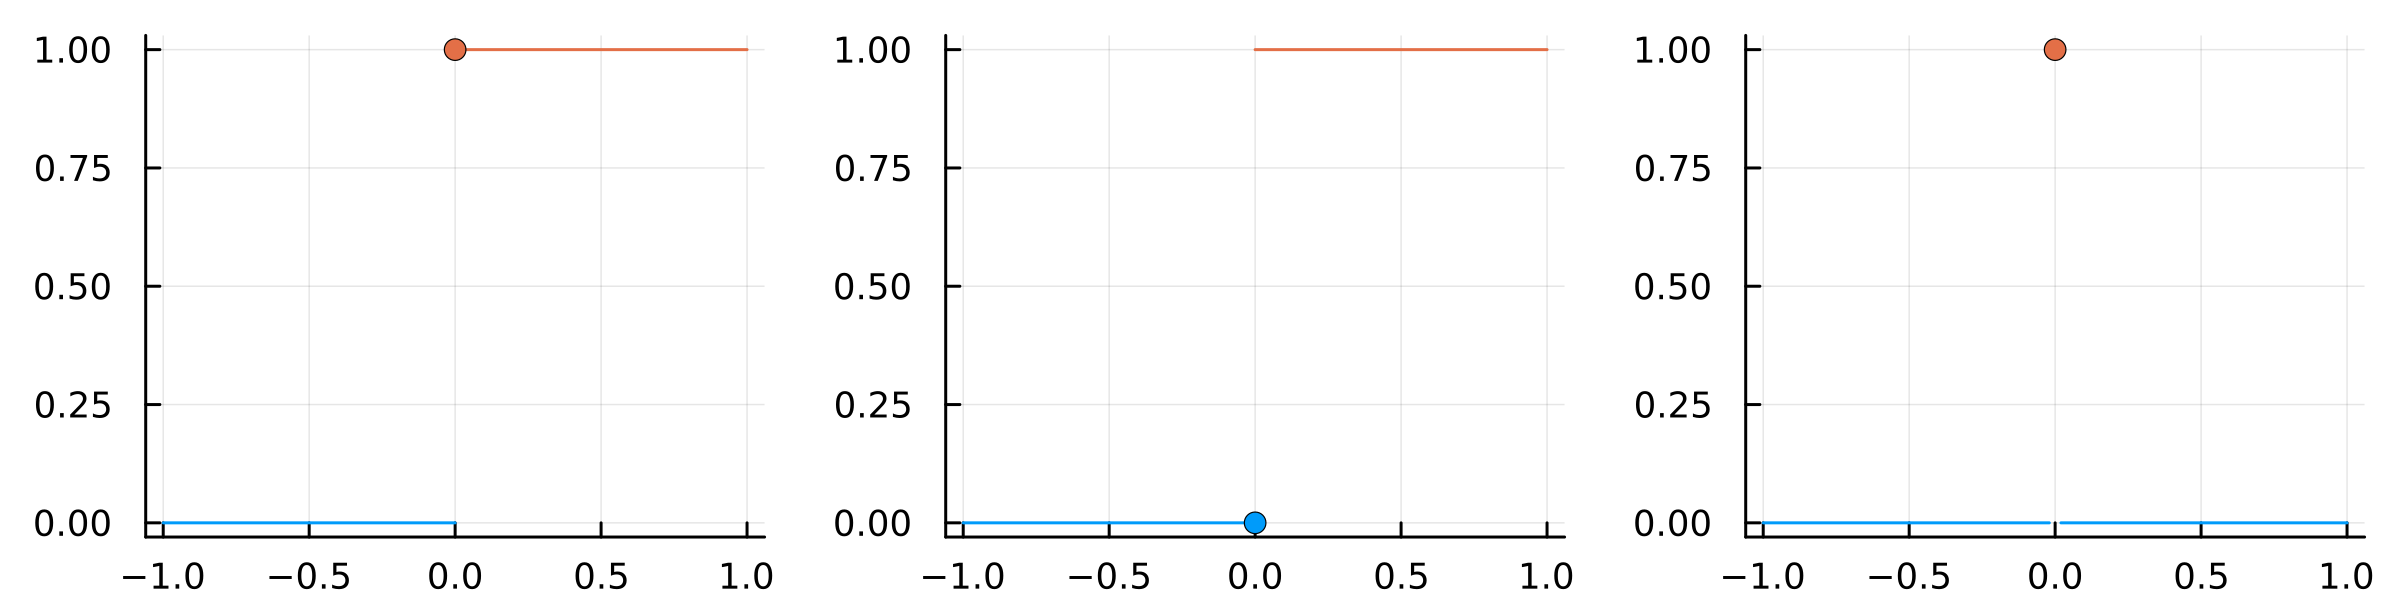
\includegraphics[scale=0.2]{figures/step-func-integrator.png}
    \caption{Left: $\alpha(x)$ is continuous from the right at $x=0$. Middle: $\alpha(x)$ is continuous from the left at $x=0$. Right: $\alpha(x)$ has a removable discontinuity at $x=0$.}
    \label{fig:9}
\end{figure}

\noindent In this case, $f$ may not be even integrable, and if it is, $\int_{a}^{b} f \; \mathrm{d}\alpha$ may not be zero.

\begin{theorem} \label{thm:24}
    Let $c \in (a, b)$. Define a function $\alpha$ on $[a, b]$ as follows. The values of $\alpha(a)$, $\alpha(b)$ and $\alpha(c)$ are chosen arbitrarily, and elsewhere
    \begin{align*}
        \alpha(x) = \begin{cases}
            \alpha(a) & a \leq x < c \\
            \alpha(b) & c < x \leq b
        \end{cases}
    \end{align*}
    Suppose $f$ is a bounded function defined on $[a, b]$ in such a way that
    \begin{enumerate}
        \item at least one of $f$ and $\alpha$ is continuous from the left at $c$, and
        \item at least one of $f$ and $\alpha$ is continuous from the right at $c$.
    \end{enumerate}
    Then, $f \in \mathfrak{R}(\alpha)$ on $[a, b]$ with 
    \begin{align}
        \int_{a}^{b} f \; \mathrm{d}\alpha
        = f(c) [\alpha(b) - \alpha(a)]
        \label{eq:40}
    \end{align}
\end{theorem}

\begin{proof}
    (Possible expressions of $S(P,f,\alpha)$) We first investigate the expression of the Stieltjes sum $S(P,f,\alpha)$. Given any partition $P$ on $[a, b]$. If $c \notin P$, then we have 
    \begin{align*}
        S(P,f,\alpha) = f(c) [\alpha(b) - \alpha(a)]
    \end{align*}
    And if $c \in P$, we have 
    \begin{align*}
        S(P,f,\alpha) 
        = f(c-\delta_1) [\alpha(c) - \alpha(a)]
        + f(c+\delta_2) [\alpha(b) - \alpha(c)]
    \end{align*}
    where $c-\delta_1$ and $c+\delta_2$ ($\delta_1, \delta_2 \geq 0$) are two points in the adjacent sub-intervals sharing the same endpoint $c$. Note that $\delta_1$ and $\delta_2$ can not be too large. In fact, they satisfy that 
    \begin{align*}
        0 \leq \delta_1, \delta_2 \leq \norm{P}
    \end{align*}
    Taking into consideration both cases, we have the following inequality for any partition $P$:
    \begin{multline}
        \abs{
            S(P,f,\alpha)
            - f(c) [\alpha(b) - \alpha(a)]
        } \\
        \leq \abs{f(c-\delta_1) - f(c)} \abs{\alpha(c) - \alpha(a)}
        + \abs{f(c+\delta_2) - f(c)} \abs{\alpha(b) - \alpha(c)}
        \label{eq:39}
    \end{multline}
    where of course $0 \leq \delta_1, \delta_2 \leq \norm{P}$. 

    \begin{note}
        In fact, the left-hand side of \eqref{eq:39} reduces to zero when $c \notin P$ and the equality holds if $c \in P$.
    \end{note}

    \par There are altogether four scenarios concerning the continuity of $f$ and $\alpha$ at point $c$, which are 
    \begin{enumerate}
        \item $\alpha(x)$ is continuous at $x=c$.
        \item $\alpha(x)$ is continuous from the right at $x=c$, and $f(x)$ is continuous from the left at $x=c$.
        \item $\alpha(x)$ is continuous from the left at $x=c$, and $f(x)$ is continuous from the right at $x=c$.
        \item $f(x)$ is continuous at $x=c$.
    \end{enumerate}

    \par (Proof of 1) If $\alpha(x)$ is continuous at $x=c$, then $\alpha$ is a constant function. In this case, $f$ is certainly integrable with respect to $\alpha$ with $\int_{a}^{b} f \; \mathrm{d}\alpha = 0$. And \eqref{eq:40} holds since its right-hand side is also zero for $\alpha(a) = \alpha(b)$.

    \par (Proof of 2) Because $\alpha(x)$ is continuous from the right at $x=c$, we have $\alpha(c) = \alpha(b)$, and the inequality \eqref{eq:39} reduces to 
    \begin{align}
        \abs{
            S(P,f,\alpha)
            - f(c) [\alpha(b) - \alpha(a)]
        }
        \leq \abs{f(c-\delta_1) - f(c)} \abs{\alpha(c) - \alpha(a)}
        \label{eq:41}
    \end{align} 
    Given $\varepsilon > 0$, since $f(x)$ is continuous from the left at $x=c$, there exists $\delta > 0$ such that 
    \begin{align}
        -\delta < x - c < 0
        \implies \abs{f(x) - f(c)} < \frac{\varepsilon}{\abs{\alpha(c) - \alpha(a)} + 1}
        \label{eq:42}
    \end{align}
    Choose a partition $P_\varepsilon$ on $[a, b]$ with $\norm{P_\varepsilon} < \delta$. Let $P \supseteq P_\varepsilon$ be an arbitrary refinement. Applying \eqref{eq:41} to $P$, we have $\delta_1 < \norm{P} \leq \norm{P_\varepsilon}<\delta$. We may then apply \eqref{eq:42}, and obtain
    \begin{multline*}
        \abs{
            S(P,f,\alpha)
            - f(c) [\alpha(b) - \alpha(a)]
        }
        \leq \abs{f(c-\delta_1) - f(c)} \abs{\alpha(c) - \alpha(a)} \\
        < \frac{\varepsilon}{\abs{\alpha(c) - \alpha(a)} + 1} \abs{\alpha(c) - \alpha(a)}
        < \varepsilon
    \end{multline*}
    This implies $f \in \mathfrak{R}(\alpha)$ on $[a, b]$, and \eqref{eq:40} holds.

    \par (Proof of 3) The proof, in this case, is similar to that of 2.

    \par (Proof of 4) Given $\varepsilon > 0$. Because $f(x)$ is continuous at $x=c$, there exists $\delta > 0$ such that 
    \begin{align}
        \abs{x - c} < \delta
        \implies \abs{f(x) - f(c)} < \frac{\varepsilon}{\abs{\alpha(c) - \alpha(a)} + \abs{\alpha(b) - \alpha(c)} + 1}
        \label{eq:43}
    \end{align}
    Choose a partition $P_\varepsilon$ with $\norm{P_\varepsilon} < \delta$. Let $P \supseteq P_\varepsilon$. Applying \eqref{eq:39} to $P$, we have $0 \leq \delta_1, \delta_2 \leq \norm{P} \leq \norm{P_\varepsilon} < \delta$. Then \eqref{eq:39} and \eqref{eq:43} yield 
    \begin{multline*}
        \abs{
            S(P,f,\alpha)
            - f(c) [\alpha(b) - \alpha(a)]
        } \\
        <   \frac{\varepsilon}{\abs{\alpha(c) - \alpha(a)} + \abs{\alpha(b) - \alpha(c)} + 1} (\abs{\alpha(c) - \alpha(a)}
        + \abs{\alpha(b) - \alpha(c)})
        < \varepsilon
    \end{multline*}
    Hence, $f \in \mathfrak{R}(\alpha)$, and \eqref{eq:40} holds. This completes the proof.
\end{proof}

It should be emphasized that there are cases where $f \in \mathfrak{R}(\alpha)$ on $[a, b]$ while the conditions in the above theorem are not satisfied.

\begin{example}
    Let 
    \begin{align*}
        f(x) = \alpha(x) = \begin{cases}
            -1 &x < 0 \\ 
            0 &x=0 \\ 
            1 &x > 0
        \end{cases}, 
        \quad x \in [-1, 1]
    \end{align*}
    Note that neither $f$ nor $\alpha$ is continuous from the left at $0$. (And also neither $f$ nor $\alpha$ is continuous from the right at $0$.) Hence, the conditions in Theorem~\ref{thm:24} are not satisfied.
    
    However, we now show that $f$ is integrable. Let $P$ be any partition on $[-1, 1]$. If $0 \notin P$, then 
    \begin{align*}
        S(P,f,\alpha) = f(0)[\alpha(1) - \alpha(-1)] = 0
    \end{align*}
    And if $0 \in P$, we then have
    \begin{align*}
        S(P,f,\alpha) = f(-\delta_1)[\alpha(0) - \alpha(-1)] + f(\delta_2)[\alpha(1) - \alpha(0)]
        = (-1)[0-(-1)] + 1 \cdot [1 - 0]
        = 0
    \end{align*}
    where $\delta_1, \delta_2 \geq 0$. Hence, $S(P,f,\alpha) = 0$ no matter what partition and representative points we choose. It follows that $f \in \mathfrak{R}(\alpha)$ on $[-1, 1]$ with $\int_{-1}^{1} f \; \mathrm{d}\alpha = 0$.
\end{example}

\begin{example}
    Let 
    \begin{align*}
        f(x) = \begin{cases}
            \frac{\abs{\sin(x)}}{x} &x \neq 0 \\
            -1 &x = 0
        \end{cases}
        \quad\text{and}\quad 
        \alpha(x) = \begin{cases}
            -1 &x < 0 \\
            1 &x \geq 0
        \end{cases},
        \quad x \in [-3\pi, 3\pi]
    \end{align*}
    Let us take for granted that the following limit exists:
    \begin{align*}
        \lim_{x \to 0} \frac{\sin (x)}{x} = 1
    \end{align*}
    Then we note that the left and right limits of $f$ both exist but are not equal. Figure~\ref{fig:10} exhibits the graphs of these two functions. 

    \begin{figure}[ht]
        \centering
        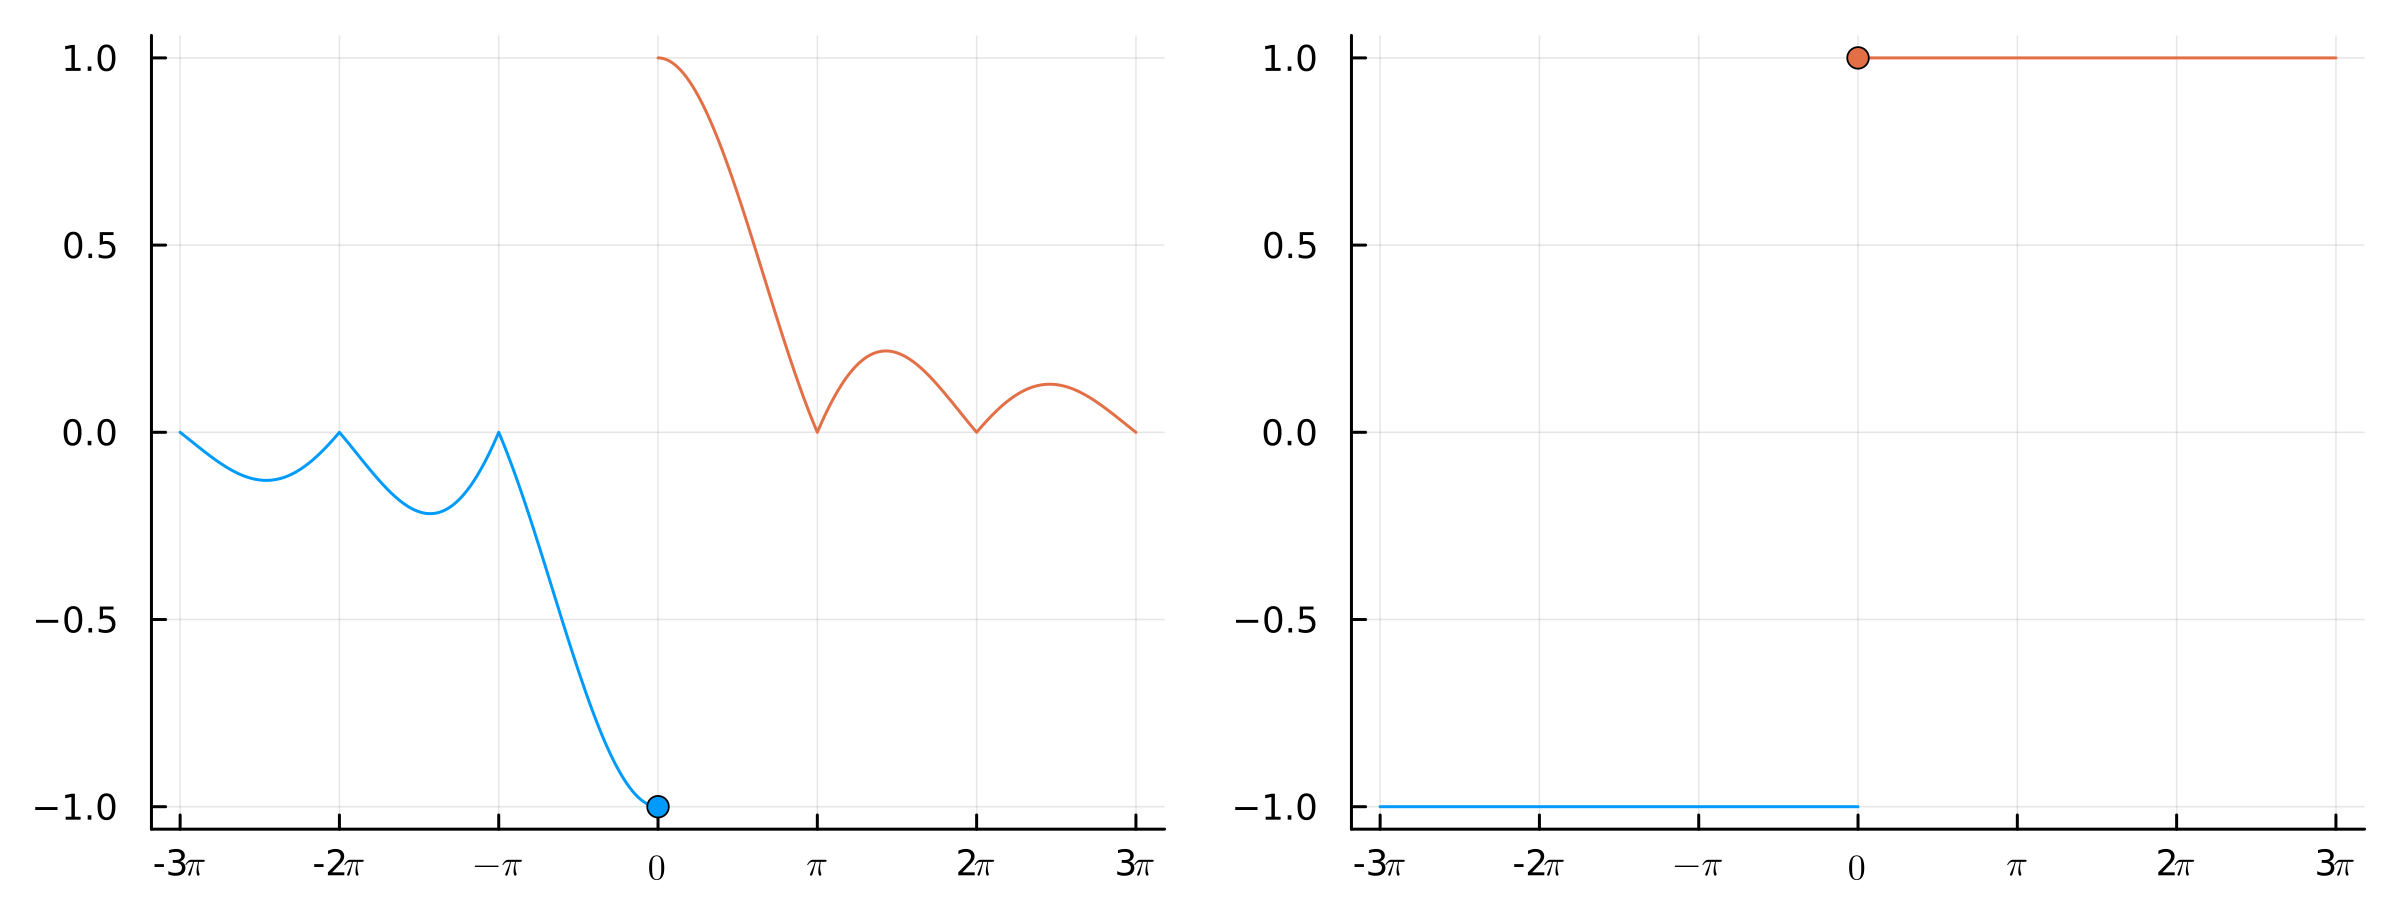
\includegraphics[scale=0.2]{figures/graph-009.png}
        \caption{Left: integrand $f$ is continuous from the left at $0$. Right: integrator $\alpha$ is continuous from the right at $0$.}
        \label{fig:10}
    \end{figure}
    
    The integrator $\alpha$ is constant except for a jump discontinuity at $0$. We note that $\alpha$ is continuous from the \textit{right} at $0$, and $f$ is continuous from the \textit{left} at $0$. Hence, the conditions in Theorem~\ref{thm:24} are satisfied, and we conclude $f \in \mathfrak{R}(\alpha)$ on $[-3\pi, 3\pi]$ with 
    \begin{align*}
        \int_{-3\pi}^{3\pi}f \; \mathrm{d}\alpha
        = f(0)[\alpha(3\pi) - \alpha(-3\pi)]
        = f(0) \cdot 2 = -2
    \end{align*} 
    \label{eg:3}
\end{example}

\begin{example}
    If we alter the function $f$ in the example above (Example~\ref{eg:3}) by re-defining $f(0) = 1$ while keeping the integrator $\alpha$ unchanged, then $f$ is no longer integrable w.r.t. $\alpha$. Now, 
    \begin{align*}
        f(x) = \begin{cases}
            \frac{\abs{\sin(x)}}{x} &x \neq 0 \\
            1 &x = 0
        \end{cases}
        \quad\text{and}\quad 
        \alpha(x) = \begin{cases}
            -1 &x < 0 \\
            1 &x \geq 0
        \end{cases},
        \quad x \in [-3\pi, 3\pi]
    \end{align*}
    Note that we cannot apply Theorem~\ref{thm:24} here since neither the integrand nor the integrator is continuous from the left of $0$.

    To show that $f$ is indeed not integrable, we consider $f$ and $\alpha$ on $[-3\pi, 0]$ and $[0, 3\pi]$ separately. It is evident that $f \in \mathfrak{R}(\alpha)$ on $[0, 3\pi]$ with $\int_{0}^{3\pi}f \; \mathrm{d}\alpha = 0$. We now consider the other half interval $[-3\pi, 0]$. Given any partition $P = \{x_0, x_1, \ldots, x_n\}$ on $[-3\pi, 0]$, we have 
    \begin{align*}
        S(P,f,\alpha)
        = f(t_n) [\alpha(x_n) - \alpha(x_{n-1})]
        = 2 f(t_n)
        = \begin{cases}
            2 \abs{\sin(t_n)} / t_n &t_n < 0\\ 
            2 &t_n = 0
        \end{cases}
    \end{align*}

    \begin{note}
        Intuitively, we know $f$ is not integrable w.r.t. $\alpha$ on $[-3\pi, 0]$ since for any partition $P$, we can always choose the last point $t_n$ such that the Stieltjes sum $S(P,f,\alpha)$ does not fall in any neighborhood of some number. But we still have to prove this rigorously by the definition.
    \end{note}

    We shall prove by contradiction. Assume $f \in \mathfrak{R}(\alpha)$ on $[-3\pi, 0]$ with $\int_{-3\pi}^{0} f \; \mathrm{d}\alpha = A$. Since $2\abs{\sin x} / x \to -2$ as $x \to 0^{-}$, there exists $\delta > 0$ such that 
    \begin{align*}
        -3 < \frac{2\abs{\sin x}}{x} < -1
        \quad \forall x \in (-\delta, 0)
    \end{align*}
    Choose $\varepsilon = 1$. For all partitions $P_\varepsilon$, we can always find a refinement $P=\{x_0, x_1, \ldots, x_n\}$ such that $x_{n-1} > -\delta$. We choose the last representative $t_n \in [x_{n-1}, x_n]$ in two ways. Letting $t_n$ be some number in that sub-interval other than $0$ yields a Riemann-Stieltjes sum in between $-3$ and $-2$, i.e., 
    \begin{align*}
        S(P,f,\alpha) = 2 \abs{\sin(t_n)} / t_n \in (-3, -1)
    \end{align*}
    since $-\delta < t_n < 0$. On the other hand, letting $t^\prime_n = 0$ leads to another Riemann-Stieltjes sum
    \begin{align*}
        S^\prime(P,f,\alpha) = 2
    \end{align*}
    We have the following inequality:
    \begin{align*}
        \abs{S(P,f,\alpha) - A} + \abs{S^\prime(P,f,\alpha) - A} 
        \geq \abs{S(P,f,\alpha) - S^\prime(P,f,\alpha)}
        > 3 > 2\varepsilon
    \end{align*}
    This implies that at least one of $\abs{S(P,f,\alpha) - A} $ and $ \abs{S^\prime(P,f,\alpha) - A} $ is greater than $\varepsilon$, which leads to a contradiction. Hence, $f$ is not integrable on $[-3\pi, 0]$.
    
    Finally, by Theorem~\ref{thm:25}, $f$ cannot be integrable with respect to $\alpha$ on the whole interval $[-3\pi, 3\pi]$.

    As a matter of fact, $f \notin \mathfrak{R}(\alpha)$ on $[-3\pi, 3\pi]$ if we re-define $f(0)$ other than $1$ while keep $\alpha$ unchanged.
    \label{eg:4}
\end{example}

\begin{exercise}
    Let $f$ be a constant function on $[a, b]$ except for \textit{finitely} many points. Show that $f$ is Riemann integrable on $[a, b]$.

    \noindent [Hint: You may find the theorem of integration by parts (Theorem~\ref{thm:20}) helpful.]
\end{exercise}

%------------------------------

\section{Reduction of Riemann-Stieltjes Integrals to Finite Sums}


%------------------------------

\section{Darboux Integrals with Monotonically Increasing Integrators}

In this section, we shall introduce another formulation of integrals, which is known as the \textbf{Darboux integrals}\index{Darboux integrals}. As we noted before, the Riemann-Stieltjes sum $S(P,f,\alpha)$ also depends on the choice of representatives, $ t_k$s. This uncertainty increases the difficulty of proving assertions related to integrals. For example, as we have seen in Example~\ref{eg:4}, it takes quite a lot of work to prove that integral does not exist. Hence, we need Darboux's formulation, which has the advantage of being easier to apply in computations or proofs. 

\begin{definition} \label{def:2}
    Let $f$ be a bounded function on $[a, b]$, and $P = \{a=x_0, x_1, \ldots, x_n=b\}$ a partition. In each sub-interval $[x_{k-1}, x_k]$, we use the symbols $M_k$ and $m_k$ to denote
    \begin{align*}
        M_k = \sup\set{f(x)}{x \in [x_{k-1}, x_k]}
        \quad\text{and}\quad
        m_k = \inf\set{f(x)}{x \in [x_{k-1}, x_k]}
    \end{align*}
    (The supremum and infimum are well-defined since we assume $f$ is bounded.) The \textbf{upper Riemann-Stieltjes sum}\index{upper Riemann-Stieltjes sum} $U(P,f,\alpha)$ and \textbf{lower Riemann-Stieltjes sum}\index{lower Riemann-Stieltjes sum} $L(P,f,\alpha)$ are defined by 
    \begin{align*}
        U(P,f,\alpha) = \sum_{k=1}^n M_k \Delta \alpha_k 
        \quad\text{and}\quad
        L(P,f,\alpha) = \sum_{k=1}^n m_k \Delta \alpha_k 
    \end{align*}
\end{definition}

If $\alpha(x) = x$, we write $U(P,f)$ and $L(P,f)$ with the specification of $\alpha$ dropped. And in this case, $U(P,f)$ and $L(P,f)$ are called the \textbf{upper and lower Darboux sum}\index{upper Darboux sum}\index{lower Darboux sum}.

\begin{note}
    From the definition, we note that, unlike $S(P,f,\alpha)$, $U(P,f,\alpha)$ and $L(P,f,\alpha)$ only depend on $P$, $f$ and $\alpha$.
\end{note}

On each sub-interval $[x_{k-1}, x_k]$, by definition, we have 
\begin{align}
    m_k \leq f(x) \leq M_k
    \quad \forall x \in [x_{k-1}, x_k]
    \label{eq:46}
\end{align}
It follows that 
\begin{align}
    L(P,f,\alpha) \leq U(P,f,\alpha)
    \label{eq:45}
\end{align}
If we pick a representative $t_k \in [x_{k-1}, x_k]$ in each interval and assume $\alpha$ is monotonically increasing, then \eqref{eq:46} yields
\begin{align*}
    L(P,f,\alpha) \leq S(P,f,\alpha) \leq U(P,f,\alpha)
\end{align*}
The following theorem states that not only $L(P,f,\alpha) \leq U(P,f,\alpha)$ for the same partition $P$, but also $L(P_1,f,\alpha) \leq U(P_2,f,\alpha)$ for any two partitions $P_1$ and $P_2$. The theorem also says the upper sums will decrease as the partition gets finer and finer while the lower sums will increase.

\begin{theorem} \label{thm:26}
    Suppose $\alpha$ is increasing on $[a, b]$. We have the following statements.
    \begin{enumerate}
        \item If $P^\prime \supseteq P$, then 
        \begin{align*}
            U(P^\prime,f,\alpha) \leq U(P,f,\alpha)
            \quad\text{and}\quad
            L(P^\prime,f,\alpha) \geq L(P,f,\alpha)
        \end{align*}
        \item For any two partitions $P_1$ and $P_2$ on $[a, b]$, we have 
        \begin{align*}
            L(P_1, f, \alpha) \leq U(P_2, f, \alpha)
        \end{align*}
    \end{enumerate}
\end{theorem}

\begin{proof}
    (Proof of 1) We only prove $U(P^\prime,f,\alpha) \leq U(P,f,\alpha)$ since the proof for lower sums is similar. Note that it suffices to prove the case where $P^\prime$ has exactly one point, say $c$, more than $P$.
    \begin{note}
        If $P^\prime$ has $m$ points more than $P$, then we can construct a chain of partitions:
        \begin{align*}
            P^\prime = P_1 \supseteq P_2 \cdots \supseteq P_m = P
        \end{align*}
        in such a way that $P_i$ has one point more than $P_{i+1}$. Then by applying the inequality $U(P_i,f,\alpha) \leq U(P_{i+1},f,\alpha)$, which is assumed proved, we obtain
        \begin{align*}
            U(P^\prime,f,\alpha) \leq U(P_2,f,\alpha) \leq \cdots \leq U(P,f,\alpha)
        \end{align*}
    \end{note}
    Suppose $P=\{x_0,x_1,\ldots,x_n\}$, and point $c$ is in between $x_{i-1}$ and $x_i$. The upper sum $U(P^\prime,f,\alpha)$ is then 
    \begin{align*}
        U(P^\prime,f,\alpha)
        = \sum_{k=1, k \neq i}^n M_k \Delta \alpha_k
            + M^\prime[\alpha(c) - \alpha(x_{i-1})]
            + M^{\prime\prime}[\alpha(x_{i})-\alpha(c)]
    \end{align*}
    where 
    \begin{align*}
        M^\prime = \sup\set{f(x)}{x \in [x_{i-1}, c]}
        \quad\text{and}\quad
        M^{\prime\prime} = \sup\set{f(x)}{x \in [c, x_i]}
    \end{align*}
    Since $M_i \geq M^\prime, M^{\prime\prime}$, we have 
    \begin{align*}
        M^\prime[\alpha(c) - \alpha(x_{i-1})]
        + M^{\prime\prime}[\alpha(x_{i})-\alpha(c)]
        \leq M_i \Delta \alpha_i
    \end{align*}
    Hence, $U(P^\prime,f,\alpha) \leq U(P,f,\alpha)$.

    (Proof of 2) Let $P$ be a common refinement of $P_1$ and $P_2$, say $P = P_1 \cup P_2$. Applying what we have just proved, it follows that 
    \begin{align*}
        L(P,f,\alpha) \geq L(P_1,f,\alpha)
        \quad \text{and} \quad
        U(P,f,\alpha) \leq U(P_2,f,\alpha)
    \end{align*}
    As noted before in \eqref{eq:45}, $L(P,f,\alpha) \leq U(P,f,\alpha)$. Therefore, 
    \begin{align*}
        L(P_1,f,\alpha) \leq L(P,f,\alpha)
        \leq U(P,f,\alpha) \leq U(P_2,f,\alpha)
    \end{align*}
\end{proof}

%------------------------------

In particular, since every partition is a refinement of the trivial partition $P_0 = \{a, b\}$, Theorem~\ref{thm:26} leads to 
\begin{align}
    \inf_{x\in[a,b]} f(x) [\alpha(b) - \alpha(a)] 
    \leq L(P_1, f, \alpha) \leq U(P_2, f, \alpha)
    \leq \sup_{x\in[a,b]} f(x) [\alpha(b) - \alpha(a)] 
    \label{eq:47}
\end{align}
What \eqref{eq:47} implies is that all the upper and lower Riemann-Stieltjes sums are bounded. Therefore, the infimum of upper sums and supremum of lower sums both exist as \textit{finite} numbers, which gives rise to the definition of \textbf{upper and lower Riemann-Stieltjes integrals}\index{upper Riemann-Stieltjes integral}\index{lower Riemann-Stieltjes integral}.

\begin{definition}
    Suppose $f$ is bounded and $\alpha$ is monotonically increasing on $[a, b]$. The upper and lower Riemann-Stieltjes integrals, written as $\upint_a^b f \; \mathrm{d}\alpha$ and $\lowint_a^b f \; \mathrm{d}\alpha$, are defined by 
    \begin{align*}
        \upint_a^b f \; \mathrm{d}\alpha
        = \inf \set{U(P,f,\alpha)}{P \in \mathcal{P}[a,b]}
        \quad \text{and} \quad
        \lowint_a^b f \; \mathrm{d}\alpha
        = \sup \set{L(P,f,\alpha)}{P \in \mathcal{P}[a,b]}
    \end{align*}
\end{definition}

%------------------------------

Sometimes, we will just say upper and lower integrals for short.

As indicated by the names, one should expect that the lower integral should be less than or equal to the upper integral. This is indeed the case.

\begin{theorem}
    Suppose $\alpha$ is increasing on $[a, b]$. We have 
    \begin{align}
        \lowint_a^b f \; \mathrm{d}\alpha
        \leq \upint_a^b f \; \mathrm{d}\alpha
        \label{eq:48}
    \end{align}
\end{theorem}

\begin{proof}
    Given $\varepsilon > 0$, there exists a partition $P_\varepsilon$ such that 
    \begin{align*}
        U(P_\varepsilon,f,\alpha) < \upint_a^b f \; \mathrm{d}\alpha + \varepsilon
    \end{align*}
    By Theorem~\ref{thm:26}, for any partition $P$, we have 
    \begin{align*}
        L(P,f,\alpha) \leq U(P_\varepsilon,f,\alpha)
    \end{align*}
    It then follows that 
    \begin{align*}
        L(P,f,\alpha) < \upint_a^b f \; \mathrm{d}\alpha + \varepsilon
        \quad \forall P \in \mathcal{P}[a,b]
    \end{align*}
    This implies that $\upint_a^b f \; \mathrm{d}\alpha + \varepsilon$ is an upper bound of all the lower Riemann-Stieltjes sums. Thus, it must be no less than their supremum, that is, 
    \begin{align*}
        \lowint_a^b f \; \mathrm{d}\alpha
        \leq
        \upint_a^b f \; \mathrm{d}\alpha + \varepsilon
    \end{align*}
    Since the above inequality holds for any positive number $\varepsilon > 0$, we have 
    \begin{align*}
        \lowint_a^b f \; \mathrm{d}\alpha
        \leq \upint_a^b f \; \mathrm{d}\alpha
    \end{align*}
\end{proof}

There exist cases where the inequality \eqref{eq:48} is strict.

\begin{example}
    Consider the Dirichlet function
    \begin{align*}
        \ind_{\Q} (x) = \begin{cases}
            1 &x \in \Q\\ 
            0 &x \notin \Q
        \end{cases}
    \end{align*}
    restricted on $[0,1]$. For any partition $P = \{0=x_0, x_1, \ldots, x_n=1\}$, the infimum of $\ind_{\Q}$ on each sub-interval $[x_{k-1}, x_k]$ is $0$. Hence, $L(P,\ind_{\Q}) = \sum_{k=1}^n 0 \cdot (x_k - x_{k-1}) = 0$, which implies the lower Darboux sum is always $0$. Therefore, the lower integral is $0$, i.e., $\lowint_0^1 \ind_\Q(x) \; \mathrm{d}x = 0$. Similarly, because the supremum of the Dirichlet function is $1$ in each sub-interval, the upper Darboux sum is always $1$. Hence, $\upint_0^1 \ind_\Q(x) \; \mathrm{d}x = 1$. In this case, the lower integral is strictly less than the upper integral.
    \label{eg:5}
\end{example}

%------------------------------

In the following theorems, we introduce some properties of upper and lower integrals.

\begin{theorem}
    Suppose that $f$ is bounded and $\alpha$ is increasing on $[a, b]$. Let $c \in (a, b)$. We have 
    \begin{enumerate}
        \item $\upint_a^b f \; \mathrm{d}\alpha = \upint_a^c f \; \mathrm{d}\alpha + \upint_c^b f \; \mathrm{d}\alpha$
        \item $\lowint_a^b f \; \mathrm{d}\alpha = \lowint_a^c f \; \mathrm{d}\alpha + \lowint_c^b f \; \mathrm{d}\alpha$
    \end{enumerate}
\end{theorem}

\begin{proof}
    We only prove 1, the equality concerning the upper integrals, since 2 can be proved similarly. 

    Given $\varepsilon > 0$, there exist a partition $P_1$ on $[a, c]$ and a partition $P_2$ on $[c, b]$ such that 
    \begin{align}
        U(P_1,f,\alpha) < \upint_a^c f \; \mathrm{d}\alpha + \varepsilon/2
        \quad \text{and} \quad
        U(P_2,f,\alpha) < \upint_c^b f \; \mathrm{d}\alpha + \varepsilon/2
        \label{eq:49}
    \end{align}
    Let $P = P_1 \cup P_2$. Note that $P$ is a partition on $[a, b]$, Furthermore, the upper Riemann-Stieltjes sum $U(P,f,\alpha)$ is given by 
    \begin{align}
        U(P,f,\alpha) = U(P_1,f,\alpha) + U(P_2,f,\alpha)
        \label{eq:50}
    \end{align}
    But 
    \begin{align}
        U(P,f,\alpha) \geq \upint_a^b f \; \mathrm{d}\alpha
        \label{eq:51}
    \end{align}
    Combining \eqref{eq:49}, \eqref{eq:50} and \eqref{eq:51} together, we have 
    \begin{align*}
        \upint_a^b f \; \mathrm{d}\alpha
        < \upint_a^c f \; \mathrm{d}\alpha + \upint_c^b f \; \mathrm{d}\alpha + \varepsilon
    \end{align*}
    Since the above inequality holds for any $\varepsilon > 0$. It follows that 
    \begin{align}
        \upint_a^b f \; \mathrm{d}\alpha
        \leq \upint_a^c f \; \mathrm{d}\alpha + \upint_c^b f \; \mathrm{d}\alpha
        \label{eq:52}
    \end{align}

    On the other hand, letting $\varepsilon > 0$ be chosen arbitrarily, there exists a partition $P$ on $[a, b]$ such that 
    \begin{align}
        U(P,f,\alpha) < \upint_a^b f \; \mathrm{d}\alpha + \varepsilon
        \label{eq:53}
    \end{align}
    We want to split $P$ into two partitions, one on $[a,c]$ and the other on $[c, b]$. But we need to ensure that $c$ is in $P$. To do so, we consider a refinement $P^\prime = P \cup \{c\}$. By Theorem~\ref{thm:26}, we know that the upper Riemann-Stieltjes sum concerning $P^\prime$ is reduced, i.e., 
    \begin{align}
        U(P^\prime,f,\alpha) \leq U(P,f,\alpha) < \upint_a^b f \; \mathrm{d}\alpha + \varepsilon
        \label{eq:54}
    \end{align}
    where the second inequality follows from \eqref{eq:53}. Let $P_1$ and $P_2$ be given by 
    \begin{align*}
        P_1 = \set{x \in P^\prime}{x \leq c}
        \quad \text{and} \quad 
        P_2 = \set{x \in P^\prime}{x \geq c}
    \end{align*}
    Note that indeed $P_1$ and $P_2$ are partitions on $[a, c]$ and $[c, b]$, respectively. We have 
    \begin{align}
        U(P^\prime,f,\alpha) = U(P_1,f,\alpha) + U(P_2,f,\alpha)
        \label{eq:55}
    \end{align}
    Moreover, The two upper Riemann-Stieltjes sums are bounded below by the corresponding upper integrals, that is, 
    \begin{align}
        U(P_1,f,\alpha) \geq \upint_a^c f \; \mathrm{d}\alpha
        \quad\text{and}\quad 
        U(P_2,f,\alpha) \geq \upint_c^b f \; \mathrm{d}\alpha
        \label{eq:56}
    \end{align}
    Then, by combining \eqref{eq:54}, \eqref{eq:55} and \eqref{eq:56}, we obtain
    \begin{align*}
        \int_a^b f \; \mathrm{d}\alpha + \varepsilon
        > \int_a^c f \; \mathrm{d}\alpha
        + \int_c^b f \; \mathrm{d}\alpha
    \end{align*}
    Similarly, since the above inequality holds for any $\varepsilon > 0$, we have 
    \begin{align}
        \int_a^b f \; \mathrm{d}\alpha
        \geq \int_a^c f \; \mathrm{d}\alpha
        + \int_c^b f \; \mathrm{d}\alpha
        \label{eq:57}
    \end{align}

    Finally, the equation 
    \begin{align*}
        \upint_a^b f \; \mathrm{d}\alpha = \upint_a^c f \; \mathrm{d}\alpha + \upint_c^b f \; \mathrm{d}\alpha
    \end{align*}
    follows from \eqref{eq:52} and \eqref{eq:57}.
\end{proof}

%------------------------------

However, some equations of integrals will not be valid for upper and lower integrals. For example, the following equation is a special case of Theorem~\ref{thm:18}.
\begin{align*}
    \int_{a}^{b} (f+g) \; \mathrm{d}\alpha
    = \int_{a}^{b} f \; \mathrm{d}\alpha
    + \int_{a}^{b} g \; \mathrm{d}\alpha
\end{align*}
It will not hold if we replace the integrals with upper and lower integrals. To fix this, we also need to replace equality with inequality, as stated in the next theorem. 

\begin{theorem}
    Suppose that $f$ and $g$ are bounded and $\alpha$ is increasing on $[a, b]$. We have 
    \begin{enumerate}
        \item $\upint_a^b (f+g) \; \mathrm{d}\alpha \leq \upint_a^b f \; \mathrm{d}\alpha + \upint_a^b g \; \mathrm{d}\alpha$
        \item $\lowint_a^b (f+g) \; \mathrm{d}\alpha \geq \lowint_a^b f \; \mathrm{d}\alpha + \lowint_a^b g \; \mathrm{d}\alpha$
    \end{enumerate}
\end{theorem}

\begin{proof}
    We only prove 1. Given $\varepsilon > 0$, there exist partitions $P_1$ and $P_2$ on $[a, b]$ such that 
    \begin{align*}
        U(P_1,f,\alpha) < \upint_a^b f \; \mathrm{d}\alpha + \varepsilon/2
        \quad \text{and} \quad
        U(P_2,g,\alpha) < \upint_a^b g \; \mathrm{d}\alpha + \varepsilon/2
    \end{align*}
    Let $P = P_1 \cup P_2$. It follows from Theorem~\ref{thm:26} that 
    \begin{align*}
        U(P,f,\alpha) \leq U(P_1,f,\alpha) < \upint_a^b f \; \mathrm{d}\alpha + \varepsilon/2
        \quad \text{and} \quad
        U(P,g,\alpha) \leq U(P_2,g,\alpha) < \upint_a^b g \; \mathrm{d}\alpha + \varepsilon/2
    \end{align*}
    Adding the two inequalities above yields 
    \begin{align}
        U(P,f,\alpha) + U(P,g,\alpha) 
        < \upint_a^b f \; \mathrm{d}\alpha +  \upint_a^b g \; \mathrm{d}\alpha + \varepsilon
        \label{eq:58}
    \end{align}

    Write $P=\{ x_0, x_1, \ldots, x_n \}$. Let $M_k$, $M_k^\prime$ and $M_k^{\prime\prime}$ denote
    \begin{align*}
        M_k &= \sup \set{f(x) + g(x)}{x \in [x_{k-1}, x_k]} \\ 
        M_k^\prime &= \sup \set{f(x)}{x \in [x_{k-1}, x_k]} \\ 
        M_k^{\prime\prime} &= \sup \set{g(x)}{x \in [x_{k-1}, x_k]}
    \end{align*}
    It is clear that 
    \begin{align*}
        M_k \leq M_k^\prime + M_k^{\prime\prime}
        \quad \forall k = 1, \ldots, n
    \end{align*}
    since $f(x) + g(x) \leq M_k^\prime + M_k^{\prime\prime} \; \forall x \in [x_{k-1}, x_k]$. It then follows that 
    \begin{align*}
        U(P,f+g,\alpha) \leq U(P,f,\alpha) + U(P,g,\alpha)
    \end{align*}
    Because $U(P,f+g,\alpha)$ is bounded below by its upper integral, we further have
    \begin{align}
        \upint_a^b (f+g) \; \mathrm{d}\alpha
        \leq U(P,f+g,\alpha) \leq U(P,f,\alpha) + U(P,g,\alpha)
        \label{eq:59}
    \end{align}

    Combining inequalities \eqref{eq:58} and \eqref{eq:59}, we obtain
    \begin{align*}
        \upint_a^b (f+g) \; \mathrm{d}\alpha
        < \upint_a^b f \; \mathrm{d}\alpha +  \upint_a^b g \; \mathrm{d}\alpha + \varepsilon
    \end{align*}
    Because the above inequality holds for any $\varepsilon > 0$, we finally have the inequality
    \begin{align*}
        \upint_a^b (f+g) \; \mathrm{d}\alpha
        \leq \upint_a^b f \; \mathrm{d}\alpha +  \upint_a^b g \; \mathrm{d}\alpha
    \end{align*}
    as desired.
\end{proof}

The following is an example where both inequalities are strict.

\begin{example}
    Let functions
    \begin{align*}
        f = \ind_\Q 
        \quad \text{and} \quad 
        g = -\ind_\Q
    \end{align*}
    be restricted on $[0, 1]$. We have calculated the upper and lower integrals of $f$ in Example~\ref{eg:5}. We can do the same for $g$ similarly. The results are as follows.
    \begin{align*}
        \upint_0^1 f(x) \; \mathrm{d}x = 1,
        \quad 
        \lowint_0^1 f(x) \; \mathrm{d}x = 0,
        \quad
        \upint_0^1 g(x) \; \mathrm{d}x = 0,
        \quad \text{and} \quad
        \lowint_0^1 g(x) \; \mathrm{d}x = -1,
    \end{align*}
    Note that the sum of the two functions is zero, i.e., $f + g = 0$. Hence, we have
    \begin{align*}
        \upint_0^1 (f+g)(x) \; \mathrm{d}x 
        = 0 
        < 1 
        = \upint_0^1 f(x) \; \mathrm{d}x + \upint_0^1 g(x) \; \mathrm{d}x \\
        \lowint_0^1 (f+g)(x) \; \mathrm{d}x 
        = 0
        > -1 
        = \lowint_0^1 f(x) \; \mathrm{d}x + \lowint_0^1 g(x) \; \mathrm{d}x
    \end{align*}
\end{example}

%------------------------------

\section{Riemann's Condition}

In Darboux's formulation, the integral exists if and only if the upper and lower integrals are equal to each other. We now show that this is equivalent to the criterion of the existence of integrals from our definition (Definition~\ref{def:1}). Furthermore, we will introduce another equivalent condition, \textbf{Riemann's condition}\index{Riemann's condition}, which is convenient to use in proofs.

\begin{definition}[Riemann's Condition]
    Suppose $f$ is bounded and $\alpha$ is increasing on $[a, b]$. Function $f$ is said to satisfy \textbf{Riemann's condition} w.r.t. $\alpha$ on $[a, b]$ if for any $\varepsilon > 0$, there exists a partition $P_\varepsilon$ on $[a, b]$ such that 
    \begin{align*}
        U(P,f,\alpha) - L(P,f,\alpha) < \varepsilon
    \end{align*}
    for any refinement $P \supseteq P_\varepsilon$.
\end{definition}

Essentially, Riemann's condition requires that the upper and lower sums should be arbitrarily close.

%------------------------------

The following states that the existence of Riemann-Stieltjes integrals, the existence of Darboux integrals and Riemann's condition are equivalent.

\begin{theorem} \label{thm:28}
    Suppose $f$ is bounded and $\alpha$ is increasing on $[a, b]$. Then the following statements are equivalent.
    \begin{enumerate}
        \item $f$ is integrable w.r.t. $\alpha$ on $[a, b]$, i.e., $f \in \mathfrak{R}(\alpha)$ on $[a, b]$.
        \item $f$ satisfies Riemann's condition w.r.t. $\alpha$ on $[a, b]$.
        \item The upper and lower integrals are equal to each other, i.e., $\upint_a^b f \; \mathrm{d}\alpha = \lowint_a^b f \; \mathrm{d}\alpha$.
    \end{enumerate}
\end{theorem}

\begin{proof}
    If $\alpha$ is constant, then this theorem holds trivially. We assume $\alpha$ is non-constant in the rest of the proof.

    (Proof of 1 $\implies$ 2) Given $\varepsilon > 0$, since $f \in \mathfrak{R}(\alpha)$, there exists a partition $P_\varepsilon$ on $[a, b]$ such that 
    \begin{align}
        \abs{S(P,f,\alpha) - \int_{a}^{b} f \; \mathrm{d}\alpha} < \varepsilon / 6
        \label{eq:60}
    \end{align}
    for any refinement $P \supseteq P_\varepsilon$ and for any choice of representative $t_k$ in each sub-interval $[x_{k-1}, x_k]$. Let this partition $P$ be fixed for now. 

    Let $M_k$ and $m_k$ be as in Definition~\ref{def:2}. We can choose each $t_k^\prime \in [x_{k-1}, x_k]$ such that 
    \begin{align*}
        M_k - \frac{\varepsilon / 3}{\alpha(b) - \alpha(a)}
        < f(t_k^\prime)
        \leq M_k
    \end{align*}
    Multiplying by $\Delta \alpha_k$ and then summing up over $k$ yields
    \begin{align}
        U(P,f,\alpha) - \varepsilon / 3
        < S^\prime(P,f,\alpha)
        \leq U(P,f,\alpha)
        \label{eq:61}
    \end{align}
    where $S^\prime(P,f,\alpha) = \sum_{k} f(t_k^\prime) \Delta\alpha_k$. We can instead choose each $t_k^{\prime\prime} \in [x_{k-1}, x_k]$ such that 
    \begin{align*}
        m_k + \frac{\varepsilon / 3}{\alpha(b) - \alpha(a)}
        > f(t_k^{\prime\prime}) 
        \geq m_k 
    \end{align*}
    Similarly, we then have 
    \begin{align}
        L(P,f,\alpha) + \varepsilon / 3
        > S^{\prime\prime}(P,f,\alpha)
        \geq L(P,f,\alpha) 
        \label{eq:62}
    \end{align}
    where $S^{\prime\prime}(P,f,\alpha) = \sum_{k} f(t_k^{\prime\prime}) \Delta\alpha_k$. By combining \eqref{eq:61} and \eqref{eq:62}, we will obtain the following two inequalities. 
    \begin{align}
        0
        \leq U(P,f,\alpha) - S^{\prime}(P,f,\alpha) 
        < \varepsilon / 3
        \label{eq:63}
    \end{align}
    \begin{align}
        0
        \leq S^{\prime\prime}(P,f,\alpha) - L(P,f,\alpha)
        < \varepsilon / 3
        \label{eq:64}
    \end{align}

    Recall the Riemann-Stieltjes sums $S^{\prime}(P,f,\alpha)$ and $S^{\prime\prime}(P,f,\alpha)$ are formed with the same partition $P$. Hence, they both satisfy \eqref{eq:61}. Their difference is then bounded by 
    \begin{align}
        \abs{S^{\prime}(P,f,\alpha) - S^{\prime\prime}(P,f,\alpha)}
        \leq \abs{S^{\prime}(P,f,\alpha) - \int_{a}^{b} f \; \mathrm{d}\alpha}
        + \abs{S^{\prime\prime}(P,f,\alpha) - \int_{a}^{b} f \; \mathrm{d}\alpha}
        < \varepsilon / 3
        \label{eq:65}
    \end{align} 

    Then, the difference between the upper and lower sums can be bounded as follows.
    \begin{alignat*}{2}
        &&\;& U(P,f,\alpha) - L(P,f,\alpha) \\
        &\leq&& \abs{U(P,f,\alpha) - S^\prime(P,f,\alpha)}
        + \abs{S^\prime(P,f,\alpha) - S^{\prime\prime}(P,f,\alpha)}
        + \abs{S^{\prime\prime}(P,f,\alpha) - L(P,f,\alpha)} \\
        &<&& \varepsilon / 3 + \varepsilon / 3 + \varepsilon / 3 \\
        &=&& \varepsilon
    \end{alignat*}
    where the last inequality follows from \eqref{eq:63}, \eqref{eq:64} and \eqref{eq:65}. Therefore, Riemann's condition is satisfied since the above inequality holds for any refinement $P$ of $P_\varepsilon$.

    (Proof of 2 $\implies$ 3) Let $\varepsilon > 0$ be arbitrary. By Riemann's condition, there exists a partition $P_\varepsilon$ such that 
    \begin{align*}
        U(P,f,\alpha) - L(P,f,\alpha) < \varepsilon
    \end{align*}
    for any refinement $P \supseteq P_\varepsilon$. Because $\upint_a^b f \; \mathrm{d}\alpha \leq U(P,f,\alpha)$ and $\lowint_a^b f \; \mathrm{d}\alpha \geq L(P,f,\alpha)$, it follows that 
    \begin{align*}
        0 \leq \upint_a^b f \; \mathrm{d}\alpha - \lowint_a^b f \; \mathrm{d}\alpha
        < \varepsilon
    \end{align*}
    Therefore, the upper and lower integrals are equal to each other since the above inequality holds for any $\varepsilon > 0$.

    (Proof of 3 $\implies$ 1) Given $\varepsilon > 0$. There exist partitions $P_1$ and $P_2$ on $[a, b]$ such that 
    \begin{align*}
        U(P_1,f,\alpha) < \upint_a^b f \; \mathrm{d}\alpha + \varepsilon
        \quad \text{and} \quad 
        L(P_2,f,\alpha) > \lowint_a^b f \; \mathrm{d}\alpha - \varepsilon
    \end{align*}
    Let $P_\varepsilon = P_1 \cup P_2$ and $P$ be any of its refinements. By Theorem~\ref{thm:26} and \eqref{eq:46}, it is clear
    \begin{align*}
        \lowint_a^b f \; \mathrm{d}\alpha - \varepsilon
        < L(P,f,\alpha)
        \leq S(P,f,\alpha)
        \leq U(p,f,\alpha)
        < \upint_a^b f \; \mathrm{d}\alpha + \varepsilon
    \end{align*}
    holds for any choice of $t_k$ in each sub-interval $[x_{k-1}, x_k]$. Since the upper and lower integrals have the same value, say $A$, it then follows that 
    \begin{align*}
        \abs{S(P,f,\alpha) - A} < \varepsilon
    \end{align*}
    Therefore, indeed $f \in \mathfrak{R}(\alpha)$. This completes the proof.
\end{proof}

As one should expect, the integral $\int_{a}^{b} f \; \mathrm{d}\alpha$ has to be equal to the upper and lower integrals whenever $f$ is integrable.

\begin{corollary}
    Suppose $\alpha$ be increasing on $[a, b]$. If $f \in \mathfrak{R}(\alpha)$ on $[a, b]$, then 
    \begin{align*}
        \int_{a}^{b} f \; \mathrm{d}\alpha
        = \upint_{a}^{b} f \; \mathrm{d}\alpha
        = \lowint_{a}^{b} f \; \mathrm{d}\alpha
    \end{align*}
\end{corollary}

\begin{proof}
    Given $\varepsilon > 0$, there exist partitions $P_1$ and $P_2$ on $[a, b]$ such that 
    \begin{align*}
        U(P_1,f,\alpha) < \upint_{a}^{b} f \; \mathrm{d}\alpha + \varepsilon
        \quad\text{and}\quad
        L(P_2,f,\alpha) > \upint_{a}^{b} f \; \mathrm{d}\alpha - \varepsilon
    \end{align*}
    Let $P_\varepsilon = P_1 \cup P_2$. For any refinement $P \supseteq P_\varepsilon$, we have 
    \begin{align*}
        \upint_{a}^{b} f \; \mathrm{d}\alpha - \varepsilon
        < L(P,f,\alpha)
        \leq S(P,f,\alpha)
        \leq U(P,f,\alpha)
        < \upint_{a}^{b} f \; \mathrm{d}\alpha + \varepsilon
    \end{align*}
    The upper and lower integrals are equal, say to $A$, by Theorem~\ref{thm:8}. It follows that 
    \begin{align*}
        \abs{S(P,f,\alpha) - A} < \varepsilon
    \end{align*}
    By Definition~\ref{def:1}, $A = \int_{a}^{b} f \; \mathrm{d}\alpha$.
\end{proof}

As an exercise, we reconsider Example~\ref{eg:4} and prove that $f$ is not integrable w.r.t. $\alpha$.

\begin{exercise}
    Let functions $f$ and $\alpha$ be given by
    \begin{align*}
        f(x) = \begin{cases}
            \frac{\abs{\sin(x)}}{x} &x \neq 0 \\
            1 &x = 0
        \end{cases}
        \quad\text{and}\quad 
        \alpha(x) = \begin{cases}
            -1 &x < 0 \\
            1 &x \geq 0
        \end{cases},
        \quad x \in [-3\pi, 3\pi]
    \end{align*}
    Show that $f \notin \mathfrak{R}(\alpha)$ on $[-3\pi, 3\pi]$.

    \noindent [Hint: $\sin x < x \; \forall x > 0$.]
\end{exercise}

\begin{solution}
    It suffices to prove $f$ is not integrable w.r.t. $\alpha$ on $[-3\pi, 0]$ since $f \in \mathfrak{R}(\alpha)$ on $[0, 3\pi]$.

    Note that For any partition $P = \{x_0, x_1, \ldots, x_n\}$ on $[-3\pi, 0]$, only the last sub-integral $[x_{n-1}, x_n = 0]$ contributes to the upper and lower sums. Furthermore, using the hint, we know 
    \begin{align*}
        M_n = 1
        \quad \text{and} \quad 
        m_n = -1
    \end{align*} 
    Then the upper and lower sums are given by
    \begin{align*}
        U(P,f,\alpha) = M_n [\alpha(0) - \alpha(x_{n-1})] = 2
        \quad\text{and}\quad
        L(P,f,\alpha) = m_n [\alpha(0) - \alpha(x_{n-1})] = -2
    \end{align*}
    Since the above equations hold for any partition $P$ on $[-3\pi, 0]$, we have 
    \begin{align*}
        \upint_{-3\pi}^0 = 2
        \quad\text{and}\quad
        \lowint_{-3\pi}^0 = -2
    \end{align*}
    Therefore, by Theorem~\ref{thm:28}, $f$ is not integrable w.r.t. $\alpha$ on $[-3\pi, 0]$, and hence on $[-3\pi, 3\pi]$.

    This proof is way cleaner than the one given in Example~\ref{eg:4} thanks to Darboux's formulation of integrals.
\end{solution}

%------------------------------

\section{Properties of Riemann-Stieltjes Integrals With Respect to Increasing Integrators}

It is much easier to study and prove some properties of the Riemann-Stieltjes integrals if we require that $\alpha$ is monotonically increasing. 

Thanks to Theorem~\ref{thm:37}, which we will prove in Section~\ref{sec:1}, almost all the properties introduced in this section can be extended with ease to integrators of bounded variation.

%------------------------------

\subsection{Integrability on Sub-Intervals}

Let $c \in (a, b)$ be a point that splits the interval into two parts. If $f$ is integrable w.r.t. $\alpha$ on the entire interval $[a, b]$, then it is also integrable on both of the sub-intervals.

\begin{lemma} \label{lem:3}
    Suppose $\alpha$ is increasing on $[a, b]$. Let $c \in (a, b)$ be an interior point. If $f \in \mathfrak{R}(\alpha)$ on $[a, b]$, then $f \in \mathfrak{R}(\alpha)$ on $[a, c]$ and $f \in \mathfrak{R}(\alpha)$ on $[c, b]$
\end{lemma}

\begin{proof}
    We only prove $f \in \mathfrak{R}(\alpha)$ on $[a, c]$. Given $\varepsilon > 0$. By Theorem~\ref{thm:28}, there exists a partition $P_\varepsilon$ on $[a, b]$ such that 
    \begin{align*}
        U(P,f,\alpha) - L(P,f,\alpha) < \varepsilon
        \quad \forall P \supseteq P_\varepsilon
    \end{align*}
    Let $P_\varepsilon^\prime = (P_\varepsilon \cup \{ c \}) \cap [a, c]$. Note that $P_\varepsilon^\prime$ is a partition on $[a, c]$. Now, let $P^\prime$ be a refinement of $ P_\varepsilon^\prime$ on $[a, c]$, and $P$ a refinement of $P_\varepsilon$ on $[a, b]$. It is evident that 
    \begin{align*}
        P^{\prime\prime} = P^\prime \cup (P \cap [c, b])
    \end{align*} 
    is a refinement of $P_\varepsilon$. Therefore, we have 
    \begin{align*}
        U(P^{\prime\prime},f,\alpha) - L(P^{\prime\prime},f,\alpha) < \varepsilon
    \end{align*}
    \begin{note}
        $P^{\prime\prime}$ can be regarded as a partition formed by adding points to $P^\prime$ that are greater than $c$.
    \end{note}
    Then it is clear 
    \begin{multline*}
        U(P^{\prime},f,\alpha) - L(P^{\prime},f,\alpha)
        = \sum_{k \text{ such that } x_k \leq c} (M_k - m_k) \Delta \alpha_k \\
        \leq \sum_{k} (M_k - m_k) \Delta \alpha_k
        \leq U(P^{\prime\prime},f,\alpha) - L(P^{\prime\prime},f,\alpha)
    \end{multline*}
    Hence,
    \begin{align*}
        U(P^{\prime},f,\alpha) - L(P^{\prime},f,\alpha) < \varepsilon
    \end{align*}
    which implies $f \in \mathfrak{R}(\alpha)$ on $[a, c]$ by Theorem~\ref{thm:28}.
\end{proof}

In fact, $f$ is integrable on all sub-intervals of $[a, b]$.


\begin{theorem} \label{thm:40}
    Suppose $\alpha$ is increasing on $[a, b]$. Let $[c, d] \subseteq [a, b]$ be a sub-interval. If $f \in \mathfrak{R}(\alpha)$ on $[a, b]$, then $f \in \mathfrak{R}(\alpha)$ on $[c, d]$.
\end{theorem}

\begin{proof}
    Without loss of generality, assume $a < c < d < b$. Lemma~\ref{lem:3} implies that $f$ is integrable w.r.t. $\alpha$ on $[a, c]$ and $[a, d]$. We then conclude the proof using Theorem~\ref{thm:18}.
\end{proof}

%------------------------------

\subsection{Comparison Theorem}

It is very common in practice to compare the values of two integrals. Intuitively,
\begin{align}
    \int_{a}^{b} f \; \mathrm{d}\alpha
    \leq \int_{a}^{b} g \; \mathrm{d}\alpha
    \label{eq:69}
\end{align}
provided that $f \leq g$ and $\alpha$ is increasing. The proof of this inequality follows from the following lemma, which says the integral of $f$ w.r.t. $\alpha$ is non-negative whenever $f$ stays non-negative and $\alpha$ is increasing on $[a, b]$. Note that this is a special case of inequality \eqref{eq:69}.

\begin{lemma} \label{lem:1}
    Suppose that $\alpha$ is increasing and $f \in \mathfrak{R}(\alpha)$ on $[a, b]$. If $f(x) \geq 0 \; \forall x \in [a, b]$, then 
    \begin{align*}
        \int_{a}^{b} f \; \mathrm{d}\alpha \geq 0
    \end{align*}
\end{lemma}

\begin{proof}
    Consider the trivial partition $P = \{a, b\}$. We have
    \begin{align*}
        L(P,f,\alpha) = \inf_{x \in [a, b]} f(x) [\alpha(b) - \alpha(a)]
        \geq 0
    \end{align*}
    It then follows that 
    \begin{align*}
        \lowint_a^b f \; \mathrm{d}\alpha
        \geq L(P,f,\alpha)
        \geq 0
    \end{align*}
    Note that $\int_{a}^{b} f \; \mathrm{d}\alpha = \lowint_a^b f \; \mathrm{d}\alpha$ since $f \in \mathfrak{R}(\alpha)$. The proof is then complete.
\end{proof}

Inequality \eqref{eq:69} can be proved easily by applying the above lemma and Theorem~\ref{thm:18}.

\begin{theorem} \label{thm:30}
    Suppose that $\alpha$ is increasing and $f, g \in \mathfrak{R}(\alpha)$ on $[a, b]$. If $f(x) \leq g(x) \; \forall x \in [a, b]$, then we have the inequality
    \begin{align*}
        \int_{a}^{b} f \; \mathrm{d}\alpha 
        \leq \int_{a}^{b} g \; \mathrm{d}\alpha
    \end{align*}
\end{theorem}

\begin{proof}
    Note that the difference $(g-f)(x) \geq 0 \; \forall x \in [a, b]$. Furthermore, $(g-f) \in \mathfrak{R}(\alpha)$ on $[a, b]$ by Theorem~\ref{thm:18}. Then Lemma~\ref{lem:1} gives 
    \begin{align*}
        \int_{a}^{b} (g-f) \; \mathrm{d}\alpha \geq 0
    \end{align*}
    Using Theorem~\ref{thm:18} again to split the integrand, we have
    \begin{align*}
        \int_{a}^{b} g \; \mathrm{d}\alpha
        - \int_{a}^{b} f \; \mathrm{d}\alpha
        \geq 0
    \end{align*}
\end{proof}

%------------------------------

\subsection{Applying Continuous Functions to Integrable Functions}

Suppose we know $f \in \mathfrak{R}(\alpha)$ on $[a, b]$. The following theorem tells us that we can produce more integrable functions by applying continuous functions to $f$.

\begin{theorem} \label{thm:29}
    Suppose that $\alpha$ is increasing and $f \in \mathfrak{R}(\alpha)$ on $[a, b]$. Let $M$ and $m$ denote the supremum and infimum of $f$ on $[a, b]$. If function $\phi: [m, M] \to \R$ is continuous, then the composite function $\phi \circ f$ is also integrable w.r.t. $\alpha$ on $[a, b]$, i.e., $\phi \circ f \in \mathfrak{R}(\alpha)$.
\end{theorem}

\begin{proof}
    In the following proof, we assume that $\alpha$ is non-constant.

    Given $\varepsilon > 0$. Since $\phi$ is uniformly continuous on $[m, M]$, there exists $\delta > 0$ such that 
    \begin{align}
        \abs{s - t} < \delta
        \implies \abs{\phi(s) - \phi(t)} < \frac{\varepsilon / 2}{\alpha(b) - \alpha(a)}
        \label{eq:70}
    \end{align}
    Suppose that $\phi$ is bounded by a positive number $A > 0$, i.e., 
    \begin{align*}
        \abs{\phi} < A
    \end{align*}
    Because $f \in \mathfrak{R}(\alpha)$, there exists a partition $P_\varepsilon$ on $[a, b]$ such that 
    \begin{align}
        U(P,f,\alpha) - L(P,f,\alpha) < \frac{\varepsilon \delta}{4A}
        \label{eq:71}
    \end{align}
    for any refinement $P \supseteq P_\varepsilon$.

    Write $P = \{x_0,x_1, \ldots, x_n\}$. We now separate the indices of sub-intervals into two sets in the following way.
    \begin{align*}
        I &= \set{k=1,\ldots,n}{M_k(f) - m_k(f) < \delta} \\ 
        J &= \set{k=1,\ldots,n}{M_k(f) - m_k(f) \geq \delta}
    \end{align*}

    We first consider the sub-intervals whose indices belong to $I$. Suppose $k \in I$. Since $M_k(f) - m_k(f) < \delta$, it follows from \eqref{eq:70} that 
    \begin{align*}
        \abs{\phi[f(s)] - \phi[f(t)]}
        < \frac{\varepsilon / 2}{\alpha(b) - \alpha(a)}
        \quad \forall s,t \in [x_{k-1}, x_{k}]
    \end{align*}
    Then by Theorem~\ref{thm:27}, we have 
    \begin{align*}
        M_k(\phi \circ f) - m_k(\phi \circ f)
        = \sup_{s,t \in [x_{k-1}, x_k]} \abs{\phi[f(s)] - \phi[f(t)]}
        \leq \frac{\varepsilon / 2}{\alpha(b) - \alpha(a)}
    \end{align*}
    Summing up over $k \in I$ yields
    \begin{align}
        \sum_{k \in I} \left[ M_k(\phi \circ f) - m_k(\phi \circ f) \right] \Delta \alpha_k
        \leq \varepsilon / 2
        \label{eq:72}
    \end{align}
    
    Now, suppose $k \in J$. Note that 
    \begin{align*}
        \sum_{k \in I} \left[ M_k(\phi \circ f) - m_k(\phi \circ f) \right] \Delta \alpha_k
        \leq U(P,f,\alpha)
        < \frac{\varepsilon \delta}{4 A}
    \end{align*}
    where the last inequality follows from \eqref{eq:71}. Because $M_k(f) - m_k(f) \geq \delta$, we have 
    \begin{align*}
        \delta \sum_{k \in I} \Delta \alpha_k
        \leq \sum_{k \in I} \left[ M_k(\phi \circ f) - m_k(\phi \circ f) \right] \Delta \alpha_k
        < \frac{\varepsilon \delta}{4 A}
    \end{align*}
    which further implies
    \begin{align}
        \sum_{k \in I} \Delta \alpha_k
        < \frac{\varepsilon}{4 A}
        \label{eq:73}
    \end{align}
    Recall that $\abs{\phi} < A$. Hence, the difference $M_k(\phi \circ f) - m_k(\phi \circ f)$ is bounded above by 
    \begin{align}
        M_k(\phi \circ f) - m_k(\phi \circ f)
        < 2A
        \label{eq:74}
    \end{align}
    Combining inequalities \eqref{eq:73} and \eqref{eq:74}, we obtain 
    \begin{align}
        \sum_{k \in I} \left[ M_k(\phi \circ f) - m_k(\phi \circ f) \right] \Delta \alpha_k
        < \varepsilon / 2
        \label{eq:75}
    \end{align}

    Note that the difference $U(P,\phi \circ f, \alpha) - L(P,\phi \circ f, \alpha)$ can be summed up as follows.
    \begin{multline*}
        U(P,\phi \circ f, \alpha) - L(P,\phi \circ f, \alpha)
        = \sum_{k=1}^n \left[ M_k(\phi \circ f) - m_k(\phi \circ f) \right] \Delta \alpha_k \\ 
        = \sum_{k \in I} \left[ M_k(\phi \circ f) - M_k(\phi \circ f) \right] \Delta \alpha_k
        + \sum_{k \in J} \left[ M_k(\phi \circ f) - m_k(\phi \circ f) \right] \Delta \alpha_k
    \end{multline*}
    Finally, by applying \eqref{eq:72} and \eqref{eq:75}, the difference of upper and lower sums are bounded by 
    \begin{align*}
        U(P,\phi \circ f, \alpha) - L(P,\phi \circ f, \alpha) < \varepsilon
    \end{align*}
    Therefore, the composite function $\phi \circ f$ satisfies Riemann's condition, and hence $\phi \circ f \in \mathfrak{R}(\alpha)$ on $[a, b]$ by Theorem~\ref{thm:28}.
\end{proof}

%------------------------------

Note that the absolute value function $\phi(x) = \abs{x}$ is continuous. Applying it to an integrable function $f \in \mathfrak{R}(\alpha)$, we immediately conclude that $\abs{f}$ is also integrable.

\begin{theorem} \label{thm:31}
    Suppose $\alpha$ is increasing. If$f \in \mathfrak{R}(\alpha)$ on $[a, b]$, then $\abs{f} \in \mathfrak{R}(\alpha)$ on $[a, b]$, and we have 
    \begin{align}
        \abs{\int_{a}^{b} f \; \mathrm{d}\alpha}
        \leq \int_{a}^{b} \abs{f} \; \mathrm{d}\alpha
        \label{eq:76}
    \end{align}
\end{theorem}

\begin{proof}
    First, we note that $\abs{f} \in \mathfrak{R}(\alpha)$ on $[a, b]$ by Theorem~\ref{thm:29} since $\phi(x) = \abs{x}$ is continuous.

    It then follows from the inequality
    \begin{align*}
        -\abs{f} \leq f \leq \abs{f}
    \end{align*}
    and Theorem~\ref{thm:30} that 
    \begin{align*}
        -\int_{a}^{b} \abs{f} \; \mathrm{d}\alpha
        = \int_{a}^{b} -\abs{f} \; \mathrm{d}\alpha
        \leq \int_{a}^{b} f \; \mathrm{d}\alpha
        \leq \int_{a}^{b} \abs{f} \; \mathrm{d}\alpha
    \end{align*}
    This completes the proof.
\end{proof}

The converse of this theorem is not true. That is, $f$ is not necessarily integrable if $\abs{f}$ is integrable.

\begin{example}
    Let 
    \begin{align*}
        f(x) = \ind_{\Q}(x) - \ind_{\R \setminus \Q}(x),
        \quad x \in [a, b]
    \end{align*}
    and $\alpha$ be any \textit{non-constant} increasing function on $[a, b]$.
    
    Note that the absolute value of $f$, $\abs{f} = 1$ is constant, and hence $f \in \mathfrak{R}(\alpha)$ on $[a, b]$. And 
    \begin{align*}
        \int_{a}^{b} f \; \mathrm{d}\alpha = 0
    \end{align*}

    But $f$ is not integrable w.r.t. $\alpha$ on $[a,b]$ since 
    \begin{align*}
        \upint_a^b f \; \mathrm{d}\alpha = \alpha(b) - \alpha(a) > 0
        \quad \text{and} \quad 
        \lowint_a^b f \; \mathrm{d}\alpha = \alpha(a) - \alpha(b) < 0
    \end{align*}
    The upper and lower integrals are not equal to each other for we have assumed $\alpha$ is non-constant.
\end{example}

\begin{exercise}
    Prove the existence of $\int_a^b \abs{f} \; \mathrm{d}\alpha$ in Theorem~\ref{thm:31} without using Theorem~\ref{thm:29}.
\end{exercise}

\begin{solution}
    % TODO
\end{solution}

%------------------------------

Put $\phi(x) = x^2$ in Theorem~\ref{thm:29}, and we will have another remarkable conclusion which says the square of $f$, $f^2$, is integrable w.r.t. $\alpha$ whenever $f \in \mathfrak{R}(\alpha)$.

\begin{theorem} \label{thm:32}
    Suppose $\alpha$ is increasing. If $f \in \mathfrak{R}(\alpha)$ on $[a, b]$, then its square $f^2$ is also integrable w.r.t. $\alpha$, i.e., $f^2 \in \mathfrak{R}(\alpha)$ on $[a, b]$.
\end{theorem}

\begin{proof}
    Because $\phi(x) = x^2$ is continuous on $\R$, it is, of course, continuous on the closed interval joining the infimum and supremum of $f$, $[m, M]$. Then by Theorem~\ref{thm:29}, $f^2 \in \mathfrak{R}(\alpha)$ on $[a, b]$. 
\end{proof}

An alternative proof without using Theorem~\ref{thm:29} is left as an exercise.

\begin{exercise}
    Prove Theorem~\ref{thm:32} without using Theorem~\ref{thm:29}. But feel free to use Theorem~\ref{thm:31}.
\end{exercise}

\begin{solution}
    % TODO
\end{solution}

%------------------------------

An immediate consequence of the above theorem is as follows, which states the product of two integrable functions is also integrable.

\begin{theorem} \label{thm:38}
    Suppose $\alpha$ is increasing. If $f, g \in \mathfrak{R}(\alpha)$ on $[a, b]$, then $fg \in \mathfrak{R}(\alpha)$ on $[a, b]$.
\end{theorem}

\begin{proof}
    Note that the product $fg$ can be written as 
    \begin{align*}
        f g = \frac{1}{4} [
            (f + g)^2 - (f - g)^2
        ]
    \end{align*}
    Then this theorem follows directly from Theorem~\ref{thm:18} and Theorem~\ref{thm:32}.
\end{proof}

%------------------------------

\subsection{Riemann-Stieltjes Integral with a Variable Upper Limit}

We know by Theorem~\ref{thm:38} that the product $fg$ is integrable w.r.t. $\alpha$ whenever $f$ and $g$ are integrable. The next theorem provides an alternative view of the integral $\int_{a}^{b} f g \; \mathrm{d}\alpha$. As we will see, we can define a function $G$ in such a way that the symbol $g \; \mathrm{d}\alpha$ in the original integral can be replaced with $\mathrm{d}G$. Or we can replace $f \; \mathrm{d}\alpha$ with $\mathrm{d}F$ by defining a function $F$.

\begin{theorem} \label{thm:39}
    Suppose that $\alpha$ is increasing, and $f, g \in \mathfrak{R}(\alpha)$ on $[a, b]$. Define 
    \begin{align*}
        F(x) = \int_{a}^{x} f \; \mathrm{d}\alpha
        \quad\text{and}\quad
        G(x) = \int_{a}^{x} g \; \mathrm{d}\alpha,
        \quad x \in [a, b]
    \end{align*}
    Then $f \in \mathfrak{R}(G)$ and $g \in \mathfrak{R}(F)$ on $[a, b]$ (of course $fg \in \mathfrak{R}(\alpha)$ by Theorem~\ref{thm:38}), and we have 
    \begin{align*}
        \int_{a}^{b} fg \; \mathrm{d}\alpha
        = \int_{a}^{b} f \; \mathrm{d}G
        = \int_{a}^{b} g \; \mathrm{d}F
    \end{align*}
\end{theorem}

\begin{proof}
    We only prove $f \in \mathfrak{R}(G)$ and $\int_{a}^{b} f g \; \mathrm{d}\alpha = \int_{a}^{b} f \; \mathrm{d}G$. Suppose $g$ is bounded by some positive number, say $A$, i.e., $\abs{g(x)} < A \; \forall x \in [a, b]$. Given $\varepsilon > 0$, since $f g \in \mathfrak{R}(\alpha)$, there exists a partition $P_\varepsilon$ on $[a, b]$ such that 
    \begin{align}
        \abs{U(P,f,\alpha) - L(P,f,\alpha)} < \varepsilon / A
        \label{eq:96}
    \end{align}
    holds for any refinement $P$ of $P_\varepsilon$. Let $P = \{x_0, x_1, \ldots, x_n\} \supseteq P_\varepsilon$ and $t_k \in [x_{k-1}, x_k]$. We have
    \begin{align}
        S(P,f, G) 
        &= \sum_k f(t_k) \Delta G \nonumber \\
        &= \sum_k f(t_k) \int_{x_{k-1}}^{x_k} g \; \mathrm{d}\alpha \nonumber \\ 
        &= \sum_k \int_{x_{k-1}}^{x_k} f(t_k) g(t) \; \mathrm{d}\alpha(t)
        \label{eq:94}
    \end{align}
    On the other hand, we can write
    \begin{align}
        \int_{a}^{b} f g  \; \mathrm{d}\alpha
        = \sum_k \int_{x_{k-1}}^{x_k} f(t) g(t) \; \mathrm{d}\alpha(t)
        \label{eq:95}
    \end{align}
    Subtracting \eqref{eq:94} and \eqref{eq:95} yields
    \begin{align*}
        S(P,f, G) - \int_{a}^{b} f g  \; \mathrm{d}\alpha
        = \sum_k \int_{x_{k-1}}^{x_k} [f(t_k) - f(t)] g(t) \; \mathrm{d}\alpha(t)
    \end{align*}
    
    It then follows from Theorem~\ref{thm:31} that 
    \begin{align*}
        \abs{S(P,f, G) - \int_{a}^{b} f g  \; \mathrm{d}\alpha}
        &\leq \sum_k \abs{
                \int_{x_{k-1}}^{x_k} [f(t_k) - f(t)] g(t) \; \mathrm{d}\alpha(t)
            } \\
        &\leq \sum_k \int_{x_{k-1}}^{x_k} \abs{f(t_k) - f(t)} \abs{g(t)} \; \mathrm{d}\alpha(t) \\
        &\leq \sum_k \int_{x_{k-1}}^{x_k} (M_k - m_k) \abs{g(t)} \; \mathrm{d}\alpha(t) \\
        &= \sum_k (M_k - m_k) \int_{x_{k-1}}^{x_k} \abs{g(t)} \; \mathrm{d}\alpha(t)
    \end{align*}
    Recall $\abs{g} \leq A$. Using Theorem~\ref{thm:30}, we obtain
    \begin{align*}
        \abs{S(P,f, G) - \int_{a}^{b} f g  \; \mathrm{d}\alpha}
        &\leq \sum_k (M_k - m_k) \int_{x_{k-1}}^{x_k} A \; \mathrm{d}\alpha(t) \\
        &= A \sum_k (M_k - m_k) \Delta\alpha_k \\ 
        &= A (U(P,f,\alpha) - L(P,f,\alpha))
    \end{align*}
    Hence, 
    \begin{align*}
        \abs{S(P,f,G) - \int_{a}^{b} f g  \; \mathrm{d}\alpha} < \varepsilon
    \end{align*}
    by \eqref{eq:96}. Therefore, $f$ is integrable w.r.t. $G$ on $[a, b]$ with $\int_{a}^{b} f \; \mathrm{d}G = \int_{a}^{b} f g  \; \mathrm{d}\alpha$.
\end{proof}

\begin{example}
    Let
    \begin{align*}
        \alpha(x)
        = \begin{cases}
            1 &x \geq 0 \\ 
            0 &x < 0
        \end{cases},
        \quad
        -1 \leq x \leq 1
    \end{align*}
    Suppose $f$ and $g$ are any two functions defined on $[-1, 1]$ being continuous from the left at $x=0$. By Theorem~\ref{thm:24} and Theorem~\ref{thm:40}, we know both functions are integrable w.r.t. $\alpha$ on $[-1, x]$ if $-1 < x \leq 1$ with 
    \begin{align*}
        F(x) = \int_{-1}^x f \; \mathrm{d}\alpha = \begin{cases}
            f(0) &x \geq 0 \\ 
            0 &x < 0
        \end{cases}
        \quad \text{and} \quad 
        G(x) = \int_{-1}^x g \; \mathrm{d}\alpha = \begin{cases}
            g(0) &x \geq 0 \\ 
            0 &x < 0
        \end{cases}
    \end{align*}
    Note that $F$ and $G$ are also step functions that are continuous from the right at $x = 0$. Hence, by applying Theorem~\ref{thm:24} again, we have 
    \begin{align*}
        \int_{-1}^{1} f \; \mathrm{d}G = f(0)g(0)
        \quad \text{and} \quad 
        \int_{-1}^{1} g \; \mathrm{d}F = f(0)g(0)
    \end{align*}

    On the other hand, since the product $f g$ is continuous from the left at $x=0$, it follows from Theorem~\ref{thm:24} that \begin{align*}
        \int_{-1}^{1} f g \; \mathrm{d}\alpha
        = f(0)g(0)
    \end{align*}

    The results agree with Theorem~\ref{thm:39} as expected.
\end{example}

%------------------------------

\section{Integrators of Bounded Variation}
\label{sec:1}

If $f \in \mathfrak{R}(\alpha_1)$ and $f \in \mathfrak{R}(\alpha_2)$ on $[a, b]$ where $\alpha_1$ and $\alpha_2$ are both increasing functions, then we know from Theorem~\ref{thm:19} that $f \in \mathfrak{R}(\alpha)$ where $\alpha = \alpha_1 - \alpha_2$. Moreover, by Theorem~\ref{thm:22}, we are immediately informed that $\alpha$ is of bounded variation. 

Now, let us think about the converse of this statement. Suppose $f \in \mathfrak{R}(\alpha)$ on $[a, b]$ where $\alpha$ if of bounded variation. Can we assert that $f \in \mathfrak{R}(\alpha_1)$ and $f \in \mathfrak{R}(\alpha_2)$ on $[a, b]$ where $\alpha_1$ and $\alpha_2$ are any increasing functions satisfying $\alpha = \alpha_1 - \alpha_2$? Unfortunately, this is not true in general. For example, the Dirichlet function $\ind_\Q$ is integrable w.r.t. $\alpha(x) = 0$ on $[0, 1]$. We can write $\alpha(x) = 0 = x - x$. But clearly $\ind_\Q \notin \mathfrak{R}$ on $[0, 1]$.

However, as the next theorem will state, $f$ is always integrable w.r.t. the total variation $V_a^x(\alpha)$ of $\alpha$ provided that $f \in \mathfrak{R}(\alpha)$.

\begin{theorem} \label{thm:37}
    If $f \in \mathfrak{R}(\alpha)$ on $[a, b]$, then $f \in \mathfrak{R}(V_a^x(\alpha))$ on $[a, b]$ where $V_a^x(\alpha)$ is the total variation of $\alpha$, which is regarded as a function of $x$ as in Definition~\ref{def:3}.
\end{theorem}

Before presenting the proof, we first introduce some notations we shall use as well as the general strategy of this proof.

For a sub-interval $[x_{k-1}, x_k]$ in the partition $P = \{ x_0, \ldots, x_n \}$ on $[a, b]$, we adopt the following notation:
\begin{align*}
    M_k = \sup_{x \in [x_{k-1}, x_k]} f(x),
    \quad
    m_k = \inf_{x \in [x_{k-1}, x_k]} f(x)
    \quad\text{and}\quad
    \Delta V_k = V_{x_{k-1}}^{x_k}(\alpha)
\end{align*}
And we write $V(x)$ instead of $V_a^x(\alpha)$ to emphasize that the total variation is a function of $x$.

Observe that $V(x)$ is monotonically increasing, hence we shall prove $f$ is integrable w.r.t. $V(x)$ mainly relies on Riemann's condition (Theorem~\ref{thm:28}). We intend to bound the difference between the upper and the lower sum, which is shown in the following, with an arbitrarily small positive number.
\begin{align*}
    U(P,f,V) - L(P,f,V)
    &= \sum_k (M_k - m_k) \Delta V_k \\ 
    &= \sum_k (M_k - m_k) \left( \Delta V_k - \abs{\Delta\alpha_k} \right)
    + \sum_k (M_k - m_k) \abs{\Delta\alpha_k}
\end{align*}
Therefore, we shall focus on bounding each of the two terms on the right-hand side of the above equation.

We now present the proof as follows.

\begin{proof}
    If $f$ is a constant function, then this theorem holds trivially. We assume that $f$ is non-constant in the rest of the proof. Let $A$ be given by 
    \begin{align*}
        A = \sup_{x \in [a, b]} f(x) - \inf_{x \in [a, b]} f(x)
    \end{align*}
    Since $f$ is non-constant, it is clear that $A > 0$.
    
    Let $\varepsilon > 0$ be chosen arbitrarily. Since $\alpha$ is of bounded variation on $[a, b]$, by the definition of total variations, there exists a partition $P^\prime_\varepsilon$ on $[a, b]$ such that 
    \begin{align}
        V_a^b(\alpha) 
        < V(P, \alpha)
        + \frac{\varepsilon}{3A}
        \quad \forall P \supseteq P^\prime_\varepsilon
        \label{eq:85}
    \end{align}
    We shall use this inequality later.

    \par Now, we prepare another inequality that will be in use. Because $f \in \mathfrak{R}(\alpha)$, there exists a partition $P^{\prime\prime}_\varepsilon$ such that
    \begin{align}
        \abs{
            \sum \left(f(s_k) - f(t_k)\right) 
            \Delta \alpha_k
        } < \frac{\varepsilon}{3}
        \quad \forall P \supseteq P^{\prime\prime}_\varepsilon
        \label{eq:86}
    \end{align}
    where $s_k$ and $t_k$ are any two points in the $k$-th subinterval of $P$.

    \par Let $P_\varepsilon = P^\prime_\varepsilon \cup P^{\prime\prime}_\varepsilon$, and let $P = \left\{x_0, \ldots, x_n\right\} \supseteq P_\varepsilon$ be a refinement. We have 
    \begin{align*}
        U(P,f,V) - L(P,f,V)
        &= \sum_{k=1}^n (M_k - m_k) \Delta V_k \\ 
        &= \sum_{k=1}^n (M_k - m_k) \left( \Delta V_k - \abs{\Delta\alpha_k} \right)
        + \sum_{k=1}^n (M_k - m_k) \abs{\Delta\alpha_k}
    \end{align*}
    Recall $A = \sup f - \inf f$. Hence, the right-hand side of the equality above can be further enlarged to
    \begin{align}
        U(P,f,V) - L(P,f,V)
        \leq A \sum_{k=1}^n \left( \Delta V_k - \abs{\Delta\alpha_k} \right)
        + \sum_{k=1}^n (M_k - m_k) \abs{\Delta\alpha_k}
        \label{eq:87}
    \end{align}
    Note that $P \supseteq P_\varepsilon \supseteq P^\prime_\varepsilon$. It then follows from \eqref{eq:85} that 
    \begin{align*}
        \sum_{k=1}^n \Delta V_k
        = V_a^b(\alpha) 
        < V(P, \alpha)
        + \frac{\varepsilon}{3A}
        = \sum_{k=1}^n \abs{\Delta\alpha_k}
        + \frac{\varepsilon}{3A}
    \end{align*}
    Rearranging the terms, we obtain 
    \begin{align}
        \sum_{k=1}^n \left( \Delta V_k - \abs{\Delta\alpha_k} \right)
        < \frac{\varepsilon}{3A}
        \label{eq:88}
    \end{align}
    By combining \eqref{eq:87} and \eqref{eq:88}, we have 
    \begin{align}
        U(P,f,V) - L(P,f,V)
        < \frac{\varepsilon}{3}
        + \sum_{k=1}^n (M_k - m_k) \abs{\Delta\alpha_k}
        \label{eq:89}
    \end{align}

    It requires much more work to bound the term $\sum_{k=1}^n (M_k - m_k) \abs{\Delta\alpha_k}$ in \eqref{eq:89}. Let $h$ be a positive number given by 
    \begin{align*}
        h = \frac{\varepsilon}{3(V_a^b (\alpha) + 1)}
    \end{align*}
    Let $I(P), J(P) \subseteq \left\{0, 1, \ldots, n\right\}$ be defined as 
    \begin{align*}
        I(P) &= \set{k}{\Delta\alpha_k \geq 0} & 
        J(P) &= \set{k}{\Delta\alpha_k < 0}
    \end{align*}

    For $k \in I(P)$, we can choose a pair of points, $s_k$ and $t_k$, in the $k$-th subinterval of $P$ such that 
    \begin{align*}
        M_k - m_k < f(s_k) - f(t_k) + h
    \end{align*}
    In this case, 
    \begin{align}
        (M_k - m_k)\abs{\Delta\alpha_k}
        < \left(f(s_k) - f(t_k) + h\right)\abs{\Delta\alpha_k}
        =  \left(f(s_k) - f(t_k) + h\right) \Delta\alpha_k
        \label{eq:90}
    \end{align}

    On the other hand, for $k \in J(P)$, we can choose a pair of points, $s_k$ and $t_k$, in the $k$-th subinterval of $P$ such that 
    \begin{align*}
        M_k - m_k < -f(s_k) + f(t_k) + h
    \end{align*}
    It then follows that
    \begin{align}
        (M_k - m_k)\abs{\Delta\alpha_k}
        < \left(-f(s_k) + f(t_k) + h\right)\abs{\Delta\alpha_k}
        =  \left(f(s_k) - f(t_k) - h\right) \Delta\alpha_k
        \label{eq:91}
    \end{align}

    Compare \eqref{eq:90} and \eqref{eq:91}, we conclude
    \begin{align*}
        (M_k - m_k)\abs{\Delta\alpha_k}
        < \left(f(s_k) - f(t_k)\right) \Delta\alpha_k
        + h \abs{\Delta\alpha_k}
        \quad \forall k \in \left\{0, 1, \ldots, n\right\}
    \end{align*}
    Therefore, 
    \begin{align*}
        \sum_{k=1}^n (M_k - m_k) \abs{\Delta\alpha_k}
        &< \sum_{k=1}^n \left(f(s_k) - f(t_k)\right) \Delta\alpha_k + h \sum_{k=1}^n \abs{\Delta\alpha_k} \\ 
        &\leq \sum_{k=1}^n \left(f(s_k) - f(t_k)\right) \Delta\alpha_k + h V_a^b (\alpha) \\ 
        &< \frac{\varepsilon}{3} + \sum_{k=1}^n \left(f(s_k) - f(t_k)\right)\Delta\alpha_k \\ 
        &\leq \frac{\varepsilon}{3} + \abs{\sum_{k=1}^n \left(f(s_k) - f(t_k)\right)\Delta\alpha_k}
    \end{align*}
    In summary,
    \begin{align}
        \sum_{k=1}^n (M_k - m_k) \abs{\Delta\alpha_k}
        < \frac{\varepsilon}{3} + \abs{\sum_{k=1}^n \left(f(s_k) - f(t_k)\right)\Delta\alpha_k}
        \label{eq:92}
    \end{align}
    Since $P \supseteq P_\varepsilon \supseteq P^{\prime\prime}_\varepsilon$, we may apply \eqref{eq:86} to \eqref{eq:92} and obtain that 
    \begin{align}
        \sum_{k=1}^n (M_k - m_k) \abs{\Delta\alpha_k}
        < \frac{\varepsilon}{3} + \frac{\varepsilon}{3}
        = \frac{2\varepsilon}{3}
        \label{eq:93}
    \end{align}

    \par Finally, by combining \eqref{eq:89} and \eqref{eq:93}, we have 
    \begin{align*}
        U(P,f,V) - L(P,f,V)
        < \frac{\varepsilon}{3} + \frac{2\varepsilon}{3}
        = \varepsilon
    \end{align*}
    Therefore, $f \in \mathfrak{R}(V(x))$ by Theorem~\ref{thm:28} since $V(x)$ is increasing.
\end{proof}

%------------------------------

\section{Existence of Riemann-Stieltjes Integrals}

%------------------------------

\subsection{Sufficient Conditions}



%------------------------------

\subsection{Necessary Conditions}

%==============================

\chapter{Sequences and Series of Functions}

%------------------------------

\section{Uniform Convergence}

As mentioned, only assuming $f_n(x) \to f(x)$ for each $x \in S$ is not enough to preserve certain properties of $f_n$. Hence, we need a stronger version of convergence than pointwise convergence. The condition $\lim_{n \to \infty} f_n(x) = f(x)$ says at a given point $x$, $f_n(x)$ will get closer and closer to $f(x)$. Chances are that $f_n(x_1)$ and $f_n(x_2)$ may not converge to $f(x_1)$ and $f(x_2)$ at the same speed. Now, we want $f_n(x)$ to get close to $f(x)$ \textit{uniformly} at the same pace for all $x \in S$. This gives rise to the definition of \textbf{uniform convergence}\index{uniform convergence}.

\begin{definition}
    Let $S$ be a subset of a metric space. A sequence of functions $\{f_n\}$ is said to converge to $f$ uniformly on $S$ if for every $\varepsilon > 0$, there exists an integer $N \in \N^\ast$ such that 
    \begin{align*}
        \abs{f_n(x) - f(x)} < \varepsilon
        \quad \forall n \geq N \;
        \forall x \in S
    \end{align*}
    Symbolically, we write $f_n \to f$ uniformly on $S$.
\end{definition}

%------------------------------

The next theorem is useful to check whether $\{f_n\}$ converges uniformly.

\begin{theorem} \label{thm:46}
    Suppose $f_n \to f$ on $S$. Then $f_n \to f$ uniformly on $S$ if and only if
    \begin{align*}
        M_n = \sup_{x \in S} \abs{f_n(x) - f(x)} < \infty
        \quad \forall n \geq N_0
    \end{align*}
    for some $N_0 \in \N^\ast$, and 
    \begin{align*}
        \lim_{n \to \infty} M_n = 0
    \end{align*}
\end{theorem}

\begin{note}
    To be clear, $M_n$ is only defined when $n \geq N_0$ for it has to be a real number.
\end{note}

\begin{proof}
    (Sufficiency) If $\lim_{n \to \infty} M_n = 0$, then for any $\varepsilon > 0$ there exists $N \in \N^\ast$ (of course, $N \geq N_0$) such that 
    \begin{align*}
        \sup_{x \in S} \abs{f_n(x) - f(x)} < \varepsilon
        \quad \forall n \geq N
    \end{align*}
    Therefore, $f_n \to f$ uniformly on $S$ by definition since $\abs{f_n(x) - f(x)} \leq \sup_{x \in S} \abs{f_n(x) - f(x)}$ for all $x \in S$.

    (Necessity) Suppose $f_n \to f$ uniformly on $S$. Given $\varepsilon > 0$, there exists $N \in \N^\ast$ such that 
    \begin{align*}
        \abs{f_n(x) - f(x)} < \varepsilon
        \quad \forall n \geq N \; 
        \forall x \in S
    \end{align*}
    Taking the supremum over $x$, we have 
    \begin{align*}
        M_n
        = \sup_{x \in S} \abs{f_n(x) - f(x)} \leq \varepsilon
        \quad \forall n \geq N
    \end{align*}
    This implies that the sequence $\{M_n\}$ converges to $0$.
\end{proof}

\begin{example}
    Let
    \begin{align*}
        f_n(x) = \frac{1}{nx},
        \quad x \in (0, 1)
    \end{align*}
    The limit of $\{f_n(x)\}$ at each $x$ is zero as $n \to \infty$. Hence, $f_n \to f = 0$. Note that 
    \begin{align*}
        \sup_{x \in (0, 1)} \abs{f_n(x) - f(x)}
        = \sup_{x \in (0, 1)} \frac{1}{nx}
        = \infty
    \end{align*}
    for every $n \in \N^\ast$. Therefore, by Theorem~\ref{thm:46}, the convergence is not uniform.
\end{example}

\begin{example}
    Let 
    \begin{align*}
        f_n(x) = \frac{1}{x} + \frac{1}{n},
        \quad x \in (0, 1)
    \end{align*}
    Note that $f(x) = \lim_{n \to \infty} f_n(x) = 1 / x$. We have
    \begin{align*}
        M_n = \sup_{x \in (0, 1)} \abs{f_n(x) - f(x)}
        = \frac{1}{n}
    \end{align*}
    Since $\lim_{n \to \infty} M_n = 0$, $f_n \to f$ uniformly on $(0, 1)$.
\end{example}

%------------------------------

A sequence of functions $\{f_n\}$ is said to be \textbf{uniformly bounded}\index{uniformly bounded functions} on $S$ if there exists a positive constant $M > 0$ such that 
\begin{align*}
    \abs{f_n(x)} \leq M
    \quad \forall n \in \N^\ast \; 
    \forall x \in S
\end{align*}


\begin{theorem}
    Suppose $\{f_n\}$ is uniformly bounded on $S$. Then $f_n \to f$ uniformly on $S$ if and only if
    \begin{align*}
        \lim_{n \to \infty} \norm{f_n - f} = 0
    \end{align*}
    where $\norm{\cdot}$ is the uniform norm on the set of bounded functions on $S$, $\mathcal{B}(S)$.
\end{theorem}


%------------------------------

Similar to the situation we encountered when dealing with numerical sequences and series, sometimes we want to prove that $\{f_n\}$ converges uniformly without knowing its limit. 

\begin{theorem}[Cauchy's Criterion] \label{thm:42}
    A sequence of functions $\{f_n\}$ converges uniformly on $S$ if and only if for any $\varepsilon > 0$, there exists $N \in N^\ast$ such that 
    \begin{align*}
        \abs{f_m(x) - f_n(x)} < \varepsilon
        \quad \forall m, n \geq N \;
        \forall x \in S
    \end{align*}
    We say $\{f_n\}$ satisfies \textbf{Cauchy's criterion}\index{Cauchy's criterion for uniform convergence} if the above condition is met.
\end{theorem}

\begin{proof}
    (Sufficiency) Suppose $\{f_n\}$ satisfies Cauchy's criterion. Fix $x \in S$, we know that the numerical sequence $\{f_n(x)\}$ is a Cauchy sequence. Hence, it has a limit, and we denote this limit by $f(x)$. In this way, we can define a function $f$ on $S$ such that 
    \begin{align*}
        f(x) = \lim_{n \to \infty} f_n(x)
        \quad \forall x \in S
    \end{align*}
    Given $\varepsilon > 0$. By Cauchy's criterion, there exists $N \in \N^\ast$ such that 
    \begin{align*}
        \abs{f_m(x) - f_n(x)} < \varepsilon / 2
        \quad \forall m, n \geq N \;
        \forall x \in S
    \end{align*}
    \begin{note}
        The reason why we choose $\varepsilon / 2$ is that when $m \to \infty$, the strict inequality will become a non-strict one.
    \end{note}
    Letting $m \to \infty$, we have
    \begin{align*}
        \abs{f(x) - f_n(x)}
        = \lim_{m \to \infty} \abs{f_m(x) - f_n(x)} \leq \varepsilon / 2
        < \varepsilon
        \quad \forall n \geq N \;
        \forall x \in S
    \end{align*}
    Therefore, $f_n \to f$ uniformly on $S$.

    (Necessity) Conversely, suppose $f_n \to f$ uniformly on $S$ for some function $f$. Given $\varepsilon > 0$, by definition, there exists $N \in \N^\ast$ such that 
    \begin{align*}
        \abs{f_n(x) - f(x)} < \varepsilon / 2
        \quad \forall n \geq N \; 
        \forall x \in S
    \end{align*}
    Let $m, n \geq N$, we have 
    \begin{align*}
        \abs{f_m(x) - f_n(x)}
        \leq \abs{f_m(x) - f(x)}
        + \abs{f_n(x) - f(x)}
        < \varepsilon / 2 + \varepsilon / 2
        = \varepsilon
        \quad \forall x \in S
    \end{align*}
    Hence, Cauchy's criterion is satisfied.
\end{proof}

%------------------------------

\section{Uniform Convergence and Continuity}

%------------------------------

If we assume $f_n$ converges to $f$ uniformly, then we can interchange the two limit processes, that is, 
\begin{align*}
    \lim_{x \to p} \lim_{n \to \infty} f_n(x)
    = \lim_{n \to \infty} \lim_{x \to p} f_n(x)
\end{align*}

\begin{theorem} \label{thm:43}
    Suppose $f_n \to f$ uniformly on $S$, and let $p$ be an accumulation point $S$. If the limit
    \begin{align*}
        A_n = \lim_{x \to p} f(x)
    \end{align*}
    exist for all $n \in \N^\ast$, then the sequence $\{A_n\}$ converges, say to $A$. Furthermore, the limit $\lim_{x \to p}f(x)$ also exists, and we have 
    \begin{align*}
        \lim_{x \to p}f(x) = A
    \end{align*}
    In other words, we can write 
    \begin{align}
        \lim_{x \to p} \lim_{n \to \infty} f_n(x)
        = \lim_{n \to \infty} \lim_{x \to p} f_n(x)
        \label{eq:97}
    \end{align}
\end{theorem}

\begin{note}
    One way to remember this theorem is that if the inner limits on both sides of \eqref{eq:97} exist, then the outer limits also exist and are equal to each other.
\end{note}

\begin{proof}
    We first show that the sequence of limits $\{A_n\}$ converges. Given $\varepsilon > 0$, by Cauchy's criterion (Theorem~\ref{thm:42}), there exists an integer $N \in \N^\ast$ such that
    \begin{align*}
        \abs{f_m(x) - f_n(x)} < \varepsilon
        \quad \forall m,n \geq N \; \forall x \in S
    \end{align*}
    Note that the absolute value function is continuous and both $f_m(x)$ and $f_n(x)$ have limits at point $p$. Using the rules of computing limits, we obtain
    \begin{align*}
        \varepsilon \geq \lim_{x \to p} \abs{f_m(x) - f_n(x)}
        = \abs{ \lim_{x \to p} f_m(x) - \lim_{x \to p} f_n(x) }
        = \abs{A_m - A_n}
    \end{align*}
    Therefore $\{A_n\}$ indeed converges by Cauchy's criterion for sequences. Let $A$ denote the limit of $\{A_n\}$.

    Next, we shall prove $f(x)$ has a limit as $ x \to p$. We choose (another) arbitrary positive number $\varepsilon > 0$. Since $f_n \to f$ uniformly on $S$, there exist $N_1 \in \N^\ast$ such that 
    \begin{align}
        \abs{f(x) - f_n(x)} < \varepsilon
        \quad \forall n \geq N_1
        \label{eq:98}
    \end{align}
    Meanwhile, since we have proved $\{A_n\}$ converges to $A$, there exist $N_2 \in \N^\ast$ such that 
    \begin{align}
        \abs{A_n - A}
        < \varepsilon / 3
        \quad \forall n \geq N_2
        \label{eq:99}
    \end{align}
    Let $N = \max\{N_1, N_2\}$. Because the limit of $\lim_{x \to p} f_N(x) = A_N$, there exist a neighborhood $V$ of $p$ in which
    \begin{align}
        \abs{f_N(x) - A_n} < \varepsilon / 3
        \quad \forall x \in V \cap S
        \label{eq:100}
    \end{align}
    We have 
    \begin{align*}
        \abs{f(x) - A}
        \leq \abs{f(x) - f_N(x)}
        + \abs{f_N(x) - A_N}
        + \abs{A_N - A}
        < \varepsilon
        \quad \forall x \in V \cap S
    \end{align*}
    where the last inequality follows from \eqref{eq:98}, \eqref{eq:99} and \eqref{eq:100}. This completes the proof.
\end{proof}

%------------------------------

The version of Theorem~\ref{thm:43} concerning the series of functions is as follows.

\begin{theorem} \label{thm:65}
    Suppose $\sum f_n \to f$ uniformly on $S$. If $f_n$ is continuous on $S$ for every $n \in \N^\ast$, then $f$ is also continuous on $S$. In particular, if $p$ is an accumulation point $S$, then 
    \begin{align*}
        \lim_{x \to p} \sum_{n=1}^\infty f_n(x)
        = \sum_{n=1}^\infty \lim_{x \to p} f_n(x)
    \end{align*}
\end{theorem}

%------------------------------

\section{Uniform Convergence and Differentiation}

In this section, we study the conditions that allow us to swap the limit and derivative symbols:
\begin{align}
    \odvs{\lim_{n \to \infty} f_n(x)}{x}
    = \lim_{n \to \infty} \odvs{f_n(x)}{x}
    \label{eq:104}
\end{align}

However, assuming $f_n \to f$ uniformly on $S$ is not sufficient to guarantee that \eqref{eq:104} holds. The following is an example.

\begin{example}
    Let 
    \begin{align*}
        f_n(x) = \frac{\sin nx}{\sqrt{n}}, 
        \quad x \in \R
    \end{align*}
    Because $\abs{\sin nx}$ is bounded by $1$ and $1 / \sqrt{n} \to 0$ as $n \to \infty$, the limit of $f_n$ is $f(x) = 0$. Note that 
    \begin{align*}
        M_n = \sup_{x \in \R} \abs{f_n(x) - f(x)}
        = \sup_{x \in \R} \frac{\abs{\sin nx}}{\sqrt{n}}
        = \frac{1}{\sqrt{n}}
    \end{align*}
    Since $\lim_{n \to \infty} M_n = 0$, $f_n \to f$ uniformly on $\R$.

    It is clear $f^\prime(x) = 0$. We now show that the limiting derivative of $f_n$ is not $f^\prime$ in general. We have 
    \begin{align*}
        f^\prime_n(x) = \sqrt{n} \cos nx
    \end{align*}
    We note that the limit of $f^\prime_n(x)$ will not exist as a finite number for most of $x$s as $n \to \infty$. In particular, $f^\prime_n(0) = \sqrt{n}$ and hence $\lim_{n \to \infty} f^\prime_n(0) = \infty$. A plot of $f_n$ and $f^\prime_n$ is shown in Figure~\ref{fig:11}.

    \begin{figure}[ht]
        \centering
        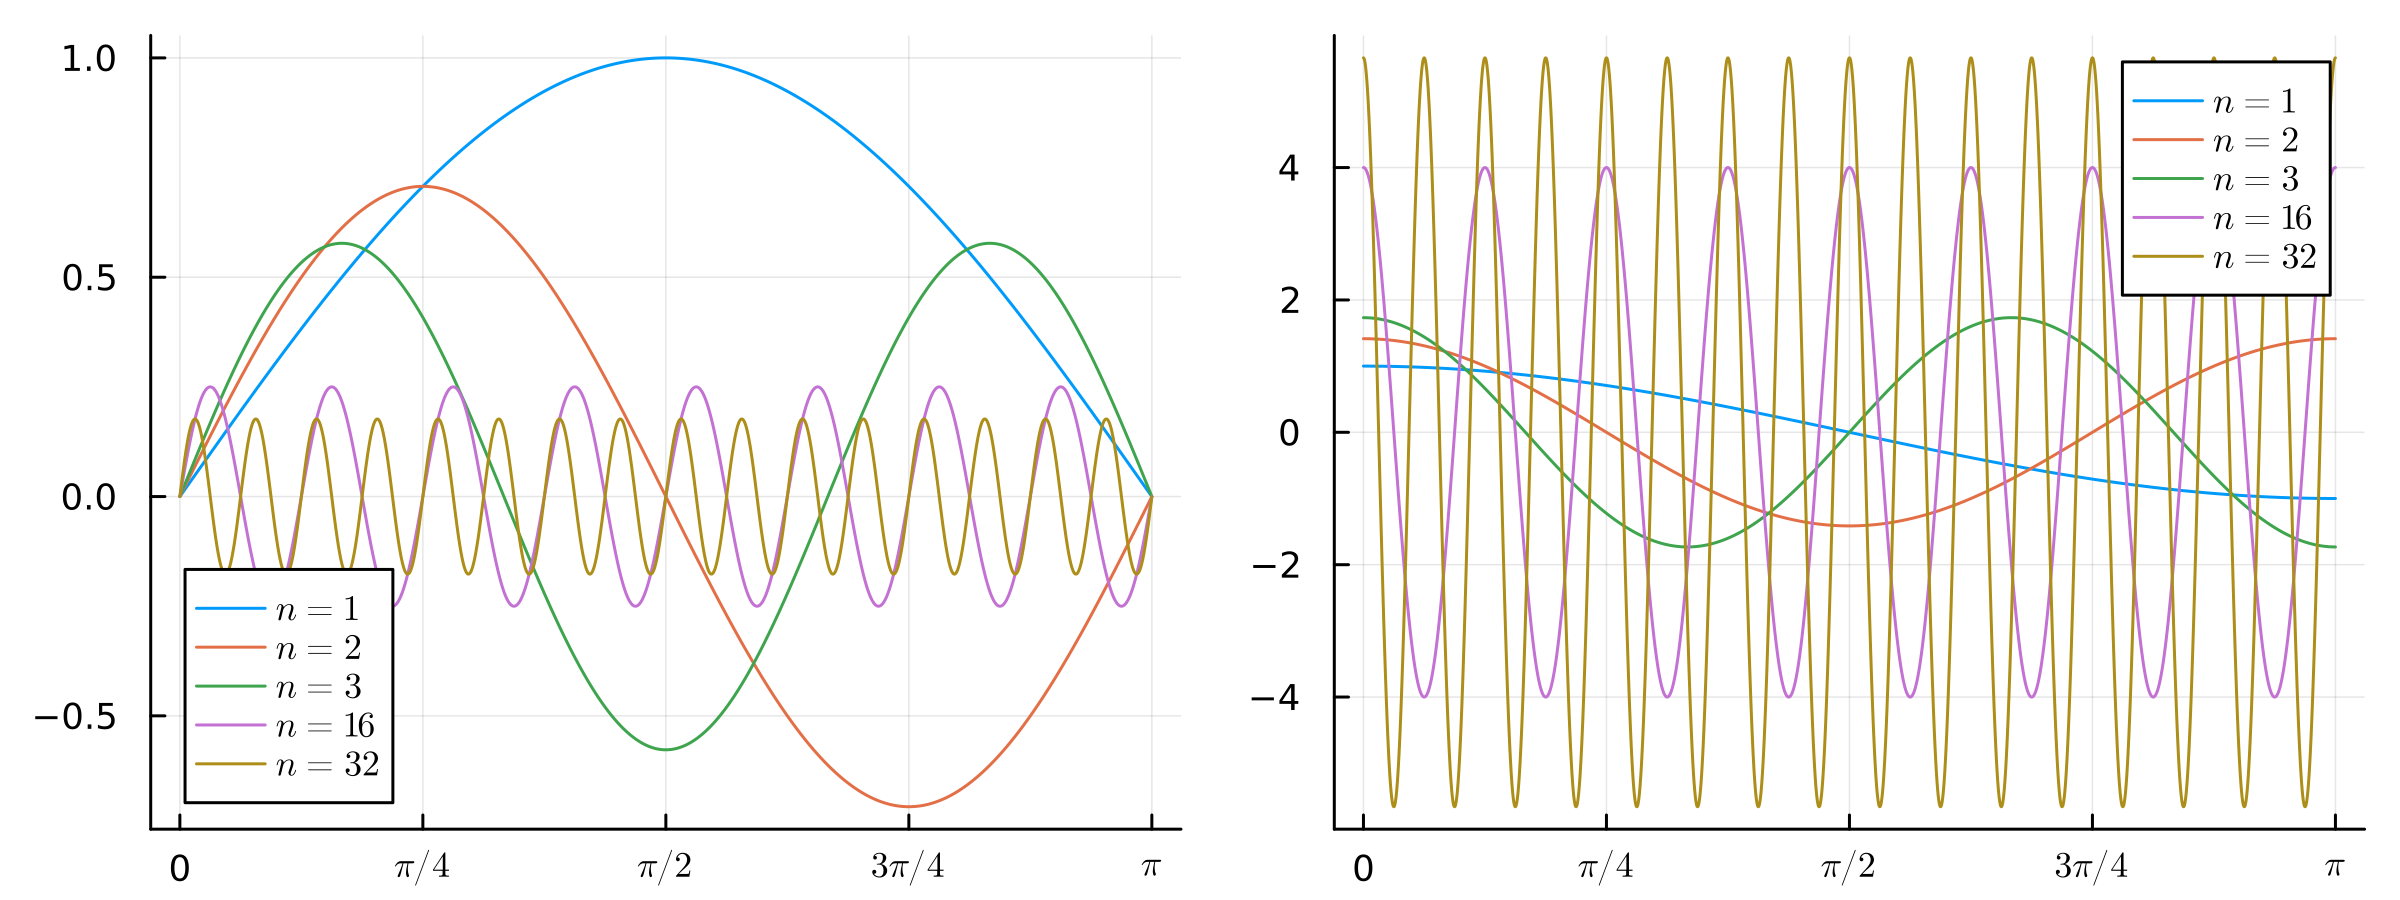
\includegraphics[scale=0.2]{figures/graph-010.png}
        \caption{Left: $f_n(x) = (\sin nx) / \sqrt{n}$. Right: $f^\prime_n(x)$.}
        \label{fig:11}
    \end{figure}
\end{example}

\begin{theorem} \label{thm:44}
    Let $\{f_n\}$ be a sequence of real-valued functions each of which has a finite derivative at every point in $(a, b)$. Suppose there exists a point $x_0 \in (a, b)$ such that the numerical sequence $\{f_n(x_0)\}$ converges. Suppose further that there exists a function $g$ such that $f^\prime_n \to g$ uniformly on $(a, b)$. Then 
    \begin{enumerate}
        \item there exists a function $f$ such that $f_n \to f$ uniformly on $(a, b)$, and
        \item $f^\prime(x)$ exists everywhere in $(a, b)$ with $f^\prime(x) = g(x)$.
    \end{enumerate}
    In this case, we can write
    \begin{align*}
        \odvs{\lim_{n \to \infty} f_n(x)}{x}
        = \lim_{n \to \infty} \odvs{f_n(x)}{x}
    \end{align*}
\end{theorem}

\begin{proof}
    We first show that $\{f_n\}$ converges uniformly on $(a, b)$. Given $\varepsilon > 0$, since $\{f_n(x_0)\}$ converges, by Cauchy's criterion for sequences,
    \begin{align}
        \abs{f_m(x_0) - f_n(x_0)} < \varepsilon / 2
        \quad \forall m,n \geq N_1
        \label{eq:101}
    \end{align}
    for some integer $N_1 \in \N^\ast$. Meanwhile, since $f^\prime_n \to g$ uniformly on $(a, b)$, it follows from Cauchy's criterion for uniform convergence (Theorem~\ref{thm:42}) that there exists $N_2 \in \N^\ast$ such that
    \begin{align}
        \abs{f^\prime_m(x) - f^\prime_n(x)} < \frac{\varepsilon / 2}{\abs{x - x_0} + 1}
        \quad \forall m, n \geq N_2 \;
        \forall x \in (a, b)
        \label{eq:102}
    \end{align}
    Let $N = \max\{N_1, N_2\}$ and let $m, n \geq N$. Define function $h$ by 
    \begin{align*}
        h(x) = f_m(x) - f_n(x)
    \end{align*}
    Applying the mean value theorem (Theorem~\ref{thm:8}) to $h$, we obtain
    \begin{align*}
        [f_m(x) - f_n(x)] - [f_m(x_0) - f_n(x_0)]
        = [f^\prime_m(\xi) - f^\prime_n(\xi)] (x - x_0)
    \end{align*} 
    where $x \neq x_0$ and $\xi$ is some number in between $x$ and $x_0$. We can then use \eqref{eq:101} and \eqref{eq:102} to bound the value of $\abs{f_m(x) - f_n(x)}$ ($x \neq x_0$) as follows:
    \begin{align*}
        \abs{f_m(x) - f_n(x)}
        &\leq \abs{f_m(x_0) - f_n(x_0)}
        + \abs{f^\prime_m(\xi) - f^\prime_n(\xi)} \abs{x - x_0} \\
        &\leq \varepsilon / 2 + \frac{\varepsilon / 2}{\abs{x - x_0} + 1} \cdot \abs{x - x_0} \\ 
        &< \varepsilon 
        \quad \forall m,n \geq N \;
        \forall x \in (a, b) \setminus \{x_0\}
    \end{align*}
    But since $m,n \geq N \geq N_1$, the inequality
    \begin{align*}
        \abs{f_m(x_0) - f_n(x_0)} < \varepsilon / 2 < \varepsilon
    \end{align*}
    also holds by \eqref{eq:101}. Therefore, we have
    \begin{align*}
        \abs{f_m(x) - f_n(x)}
        < \varepsilon
        \quad \forall m,n \geq N \;
        \forall x \in (a, b)
    \end{align*}
    which implies that $\{f_n\}$ converges uniformly on $(a, b)$. Suppose that the limit function is $f$.

    Let $c \in (a, b)$. By Theorem~\ref{thm:1}, there exists a continuous function $\phi$ defined on $(a, b)$ such that
    \begin{align*}
        f_n(x) - f_n(c) = (x - c) \phi_n(x)
    \end{align*}
    with $\phi_n(c) = f^\prime_n(c)$, i.e., 
    \begin{align*}
        \lim_{x \to c} \phi_n(x)=  f^\prime_n(c)
    \end{align*}
    \begin{note}
        We want to show 
        \begin{align*}
            \lim_{x \to c} \lim_{n \to \infty} \phi_n(x)
            = \lim_{n \to \infty} \lim_{x \to c} \phi_n(x)
        \end{align*}
        using Theorem~\ref{thm:43}.
    \end{note}
    Note that $\lim_{n \to \infty}\phi_n(x)$ exists, and 
    \begin{align*}
        \lim_{n \to \infty}\phi_n(x) = \frac{f(x) - f(c)}{x - c} =: \phi(x)
    \end{align*}
    We claim that $\phi_n \to \phi$ uniformly on $(a, b)$. The proof of this assertion is left as an exercise. (See Exercise~\ref{ex:4}.) Since both the limits $\lim_{x \to c} \phi_n(x)$ and $\lim_{n \to \infty} \phi_n(x)$ exist, and $\phi_n(x)$ converges uniformly on $(a, b)$, by Theorem~\ref{thm:43}, the limits $\lim_{n \to \infty} f^\prime_n(c)$ and $\lim_{x \to c} [f(x) - f(c)] / (x - c)$ both exist and are equal to each other, that is, 
    \begin{align*}
        \lim_{x \to c} \frac{f(x) - f(c)}{x - c}
        = \lim_{n \to \infty} f^\prime_n(c)
    \end{align*}
    Therefore, $f$ has a derivative at $c$, and 
    \begin{align*}
        f^\prime(c) = \lim_{n \to \infty} f^\prime_n(c) = g(c)
    \end{align*}
    This completes the proof.
\end{proof}

\begin{exercise}
    Complete the above proof by showing $\phi_n \to \phi$ uniformly on $(a, b)$.
    \label{ex:4}
\end{exercise}

\begin{solution}
    Given $\varepsilon > 0$, since $f_n \to f$ uniformly on $(a, b)$, there exist an integer $N \in \N^\ast$ such that 
    \begin{align*}
        \abs{f_n(x) - f(x)} < (b - a) \varepsilon / 2
        \quad \forall n \geq N \;
        \forall x \in (a, b)
    \end{align*}
    Let $n \geq N$. We then have
    \begin{align*}
        \abs{\phi_n(x) - \phi(x)}
        &\leq \frac{\abs{ [f_n(x) - f(x)] - [f_n(c) - f(c)] }}{\abs{x - c}} \\ 
        &\leq \frac{\abs{f_n(x) - f(x)} + \abs{f_n(c) - f(c)}}{b - a} \\
        &< \frac{(b - a) \varepsilon / 2 + (b - a) \varepsilon / 2}{b - a} \\
        &= \varepsilon
    \end{align*}
    Because 
    \begin{align*}
        \abs{\phi_n(x) - \phi(x)} < \varepsilon
    \end{align*}
    holds for all $n \geq N$ and for all $x \in (a, b)$, we conclude that $\phi_n \to \phi$ uniformly on $(a, b)$.
\end{solution}

%------------------------------

The following theorem is another version of Theorem~\ref{thm:44} in terms of a series of functions $\sum f_n$.

\begin{theorem} \label{thm:45}
    Let $\sum f_n$ be a series of real-valued functions each of which has a finite derivative at every point in $(a, b)$. Suppose there exists a point $x_0 \in (a, b)$ such that the numerical series $\sum f_n(x_0)$ converges. Suppose further that there exists a function $g$ such that $\sum f^\prime_n \to g$ uniformly on $(a, b)$. Then 
    \begin{enumerate}
        \item there exists a function $f$ such that $\sum f_n \to f$ uniformly on $(a, b)$, and
        \item $f^\prime(x)$ exists everywhere in $(a, b)$ with $f^\prime(x) = g(x)$.
    \end{enumerate}
    In this case, we can write
    \begin{align}
        \odvs{\sum f_n(x)}{x}
        = \sum \odvs{f_n(x)}{x}
        \label{eq:103}
    \end{align}
\end{theorem}

\begin{note}
    Equation \eqref{eq:103} is also known as \textbf{term-by-term differentiation}\index{term-by-term differentiation}.
\end{note}

%------------------------------

\section{Power Series} \label{sec:2}

A \textbf{power series}\index{power series} (in variable $z \in \C$) has the form 
\begin{align*}
    \sum_{n=0}^\infty a_n (z - z_0)^n
\end{align*}
where $a_n \in \C$ is called the coefficient of the $n$-th term, and $z_0 \in \C$ is often referred to as the center of the series. 

With every power series, there is associated a \textbf{disk of convergence}\index{disk of convergence} such that the series converges if $\abs{z - z_0} < r$ whereas diverges if $\abs{z - z_0} > r$. The number $r$ is called \textbf{radius of convergence}\index{radius of convergence}. If $r$ is a \textit{finite positive} number, then the disk of convergence is exactly the open ball in the complex plane with radius $r$, $B_r(z_0)$. However, we allow $r$ to take the value of $0$ or $\infty$ in extreme cases. When the power series is nowhere convergent except for $z = z_0$, then we say the radius of convergence is zero, i.e., $r = 0$. And if the power series converges everywhere in the complex plane, then we write $r = \infty$.

%------------------------------

\begin{theorem} \label{thm:66}
    Given a power series $\sum_{n=0}^\infty a_n (z - z_0)^n$, let 
    \begin{align*}
        \lambda = \limsup_{n \to \infty} \sqrt[n]{\abs{a_n}}
        \quad \text{and} \quad
        r = \frac{1}{\lambda}
    \end{align*}
    (where $r = 0$ if $\lambda = \infty$ and $r = \infty$ if $\lambda = 0$.) Then 
    \begin{enumerate}
        \item the power series converges absolutely if $\abs{z - z_0} < r$, and
        \item diverges if $\abs{z - z_0} > r$.
    \end{enumerate}
    Furthermore, the power series, regarded as a series of functions in variable $z$, converges uniformly on any compact subset $K$ interior to the disk of convergence.
\end{theorem}

\begin{proof}
    (Proof of 1 and 2) Applying the root test (Theorem~\ref{thm:55}), we find 
    \begin{align*}
        \limsup_{n \to \infty} \sqrt[n]{\abs{a_n(z - z_0)^n}}
        = \abs{z - z_0} \limsup_{n \to \infty} \sqrt[n]{\abs{a_n}}
        = \abs{z - z_0} \lambda
    \end{align*}
    We investigate the value of $\abs{z - z_0} \lambda$ case by case.

    (Case Where $\lambda = \infty$ and $r = 0$) If $\lambda = \infty$, then for any $z$ such that $\abs{z - z_0} > r = 0$, we have $\abs{z - z_0} \lambda = \infty > 1$. Hence, the power series diverges.
    \begin{note}
        Note that, in this case, statement 1 is \textbf{vacuously true} since the hypothesis $\abs{z - z_0} < r = 0$ is false. In fact, this theorem does not conclude that $\sum a_n (z-z_0)^n$ converges (absolutely) if $z = z_0$ when $\lambda = \infty$. But we know this is true.
    \end{note}

    (Case Where $\lambda = 0$ and $r = \infty$) In this case, $\abs{z - z_0} \lambda = 0$. Hence, the power series converges absolutely for any $z \in \C$. And we note that statement 2 is vacuously true in this case.

    (Case Where $0 < r < \infty$) If $\abs{z-z_0} < r$, then
    \begin{align*}
        \abs{z - z_0} \lambda
        < r \lambda
        = \frac{1}{\lambda} \cdot \lambda
        = 1
    \end{align*}
    Hence, the power series converges absolutely. And if $\abs{z-z_0} < r$, we then have
    \begin{align*}
        \abs{z - z_0} \lambda
        > r \lambda
        = \frac{1}{\lambda} \cdot \lambda
        = 1
    \end{align*}
    Therefore, it diverges when $\abs{z - z_0} > r$.

    (Proof of Uniform Convergence) We intend to prove that the power series converges uniformly using the Weierstrass M-test (Theorem~\ref{thm:56}). Define
    \begin{align*}
        g(z) = \abs{z - z_0},
        \quad z \in K
    \end{align*}
    Note that $g$ is a continuous real-valued function defined on a compact set. Hence, $g$ attains its maximum on $K$ by Theorem~\ref{thm:6}, that is, there exist $p \in K$ such that 
    \begin{align*}
        g(p) = \sup_{z \in K} g(z)
        = \sup_{z \in K} \abs{z - z_0}
    \end{align*}
    It then follows that 
    \begin{align*}
        \abs{a_n (z - z_0)^n}
        = \abs{a_n} \abs{z - z_0}^n
        \leq \abs{a_n} [g(p)]^n
        = \abs{a_n} \abs{p - z_0}^n
    \end{align*}
    Let 
    \begin{align*}
        M_n = \abs{a_n} \abs{p - z_0}^n
    \end{align*}
    Then the power series converges uniformly on $K$ if we can show that $\sum M_n$ converges. Indeed, by applying the root test, we have 
    \begin{align*}
        \limsup_{n \to \infty} \sqrt[n]{\abs{M_n}}
        = \abs{p - z_0} \limsup_{n \to \infty} \sqrt[n]{\abs{a_n}}
        = \abs{p - z_0} \lambda
        < r \lambda
        = 1
    \end{align*}
    This completes the proof.
\end{proof}

%------------------------------

\subsection{Derivatives of Power Series}

In fact, derivatives of the power series $f(z) = \sum a_n (z - z_0)^n$ exist throughout its disk of convergence. To show $f^\prime(z_1)$ exists, we need to consider the fraction 
\begin{align*}
    \frac{f(z) - f(z_1)}{z - z_1}
\end{align*}
The difficulty is that $f$ consists of terms in powers of $z - z_0$ while the denominator is $z - z_1$. What if we can rewrite $f$ by expanding it about $z_1$? Indeed, we are allowed to do so, as stated in the following theorem.

\begin{theorem} \label{thm:63}
    Suppose the series $\sum_{n=0}^\infty a_n (z - z_0)^n$ converges (absolutely) for $z \in B_R(z_0)$. Define
    \begin{align*}
        f(z) = \sum_{n=0}^\infty a_n (z - z_0)^n,
        \quad z \in B_R(z_0)
    \end{align*}
    Let $S$ be an open subset in $B_R(z_0)$ and $z_1 \in S$. Then there exists an open disk $B_r(z_1) \subset S$ in which $f$ has a power series expansion about $z_1$ of the form
    \begin{align*}
        f(z) = \sum_{k=0}^\infty b_k (z - z_1)^k
    \end{align*}
    where 
    \begin{align*}
        b_k = \sum_{n=k}^\infty \binom{n}{k} a_n (z_1 - z_0)^{n-k}
    \end{align*}
\end{theorem}

\begin{figure}[ht]
    \centering
    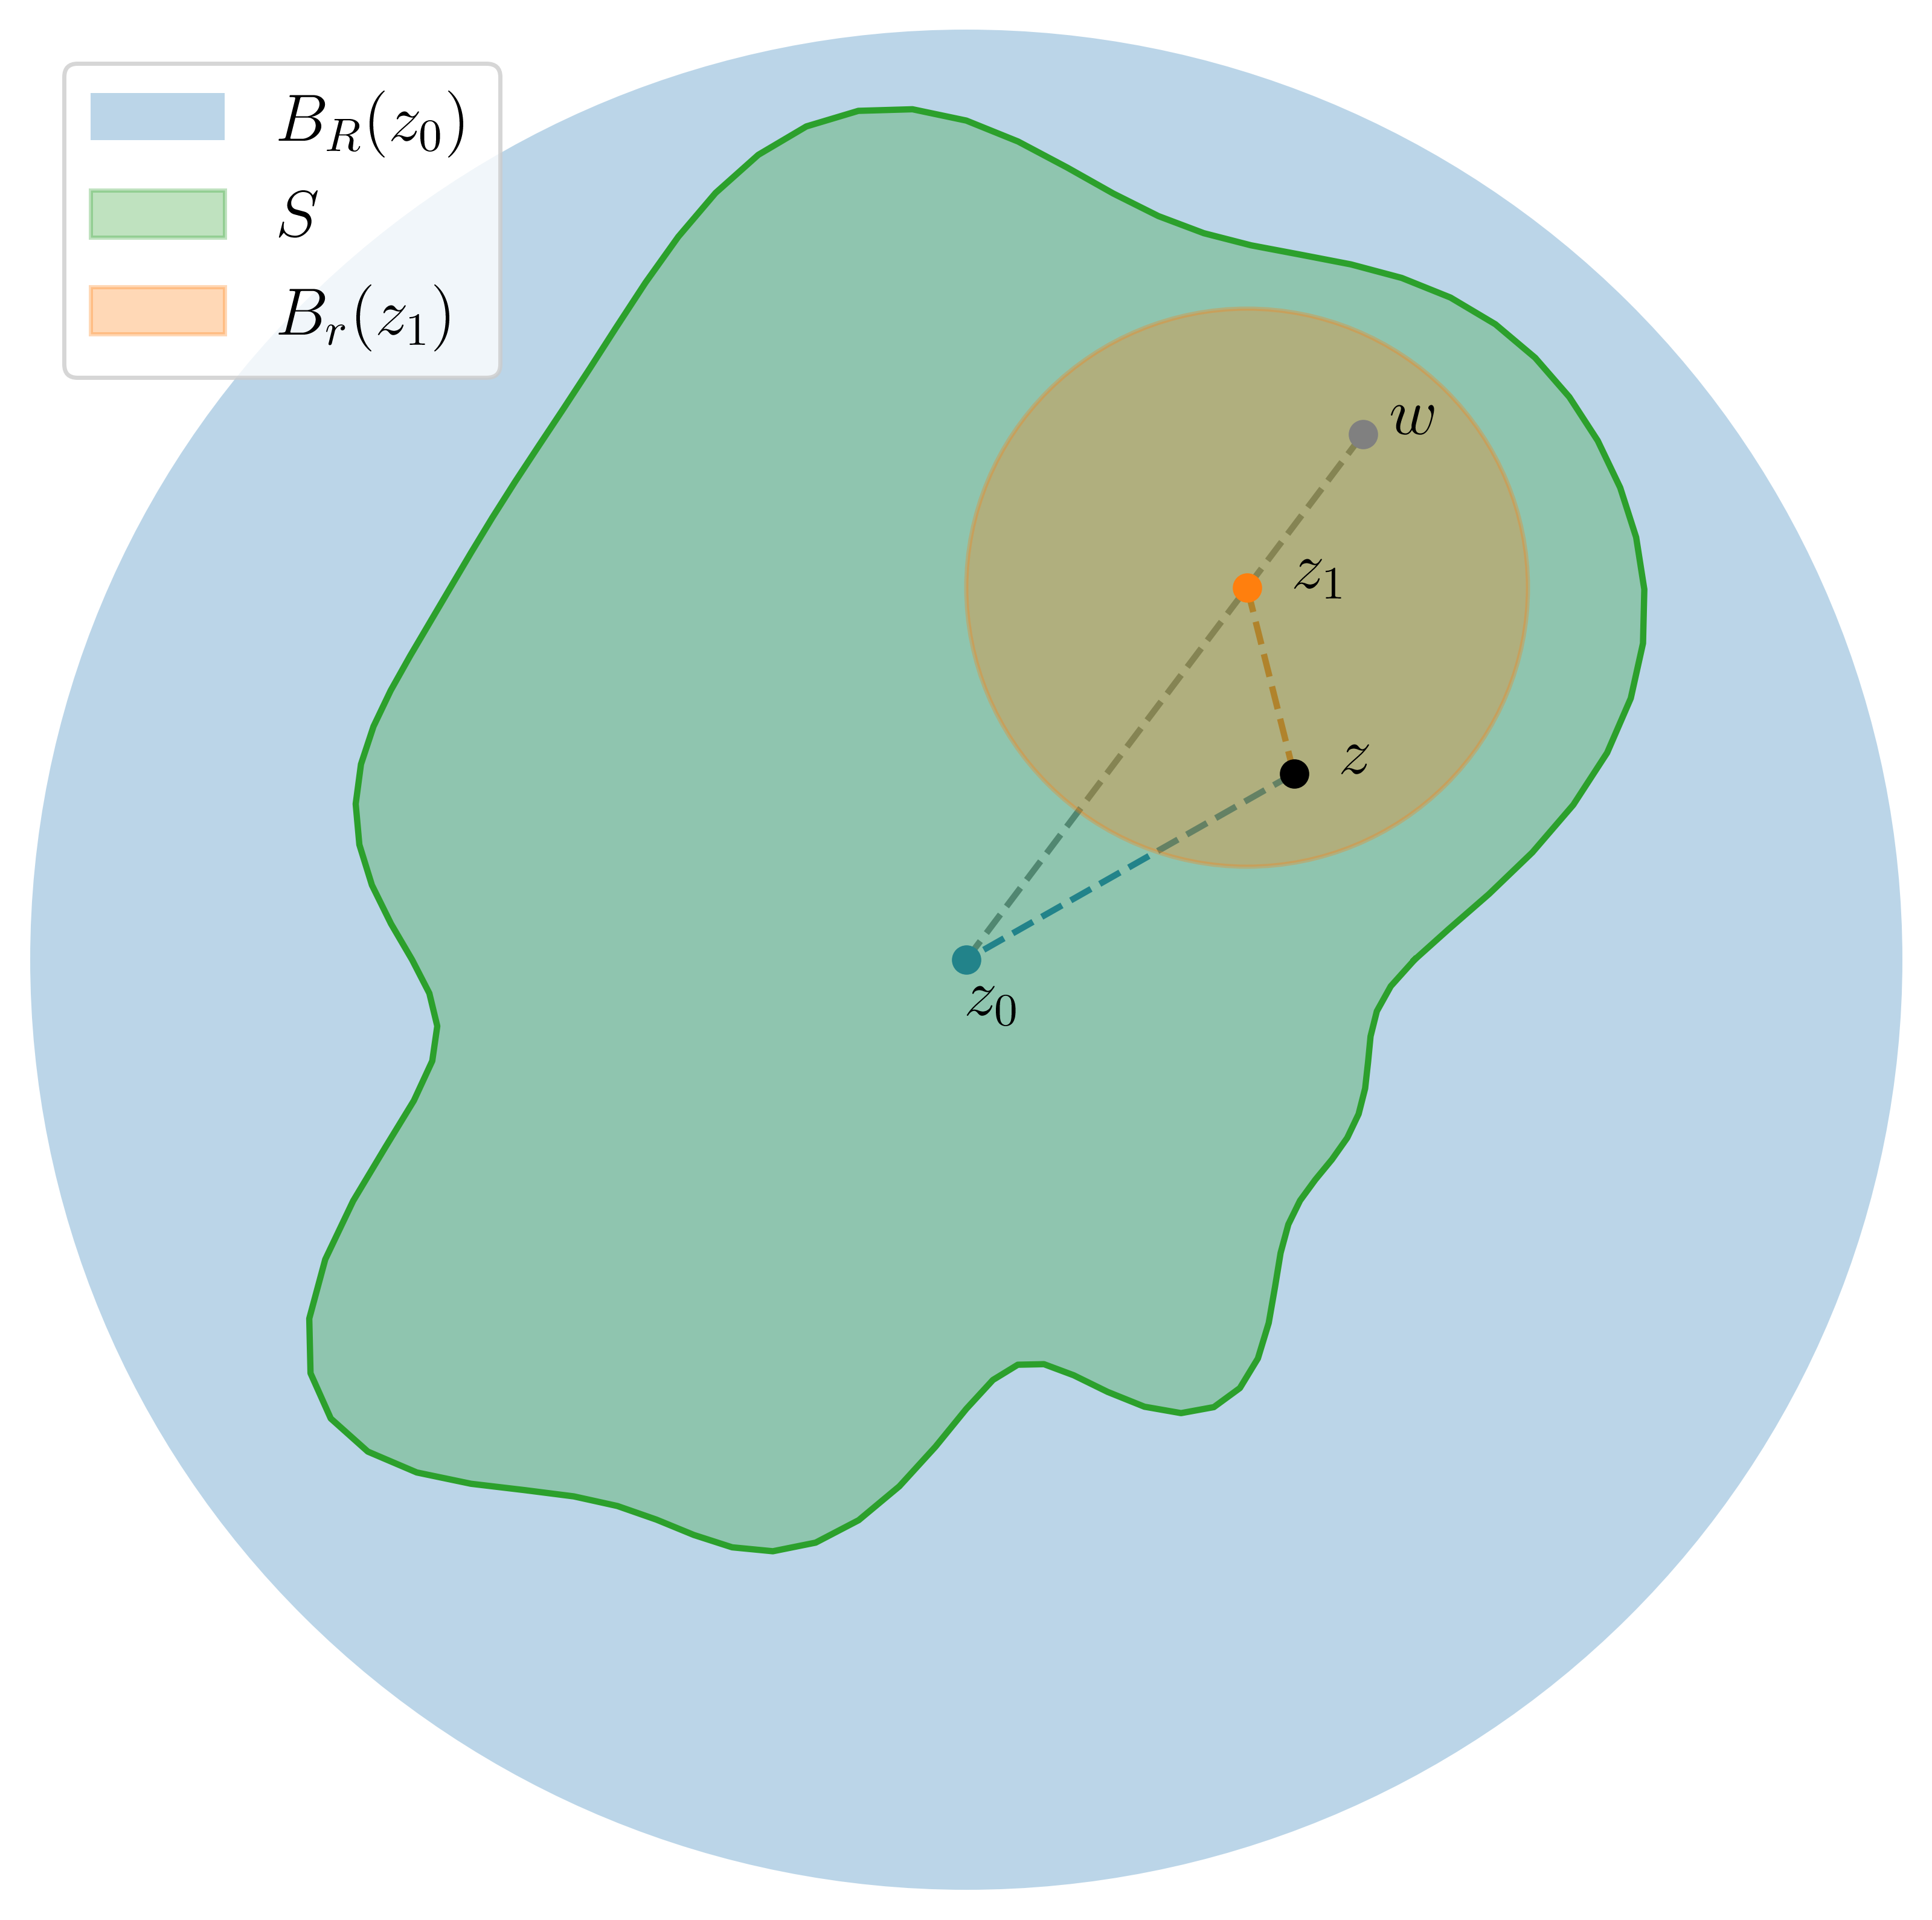
\includegraphics[scale=0.4]{figures/domain-001.png}
    \caption{Domains of power series expansions about different points.}
    \label{fig:13}
\end{figure}

\begin{proof}
    Since $S$ is open, we can find a neighborhood $B_r(z_1)$ contained in $S$. Let $z \in B_r(z_1)$. Expanding the expression $(z-z_0)^n = [(z_1 - z_0) + (z  - z_1)]^n$ in $f(z)$ using the binomial theorem, we have 
    \begin{align}
        f(z) = \sum_{n=0}^\infty a_n (z - z_0)^n
        = \sum_{n=0}^\infty a_n \sum_{k=0}^n \binom{n}{k} (z_1 - z_0)^{n-k} (z - z_1)^k
        \label{eq:126}
    \end{align}
    Define
    \begin{align*}
        c_{n,k} = \begin{cases}
            a_n \binom{n}{k} (z_1 - z_0)^{n-k} (z - z_1)^k,
            &0 \leq k \leq n \\ 
            0,
            & \text{otherwise}
        \end{cases}
    \end{align*}
    In this way, we can rewrite the right-hand side of \eqref{eq:126} as an iterated series:
    \begin{align}
        f(z) = \sum_{n=0}^\infty \sum_{k=0}^\infty c_{n,k}
        \label{eq:127}
    \end{align}
    
    We desire to interchange the order of summations in \eqref{eq:127} using Theorem~\ref{thm:61}. To do so, we need to show 
    \begin{enumerate}
        \item $\sum_{k=0}^\infty \abs{c_{n,k}}$ converges, and 
        \item $\sum_{n=0}^\infty \sum_{k=0}^\infty \abs{c_{n,k}}$ 
    \end{enumerate}
    For the first one, we note that $\sum_{k=0}^\infty \abs{c_{n,k}} = \sum_{k=0}^n c_{n,k}$ is just a finite sum. Hence, it of course converges. As for the second one, we have 
    \begin{multline*}
        \sum_{n=0}^\infty \sum_{k=0}^\infty \abs{c_{n,k}}
        = \sum_{n=0}^\infty \abs{a_n} \sum_{k=0}^n \binom{n}{k} \abs{z_1 - z_0}^{n-k} \abs{z - z_1}^k \\
        = \sum_{n=0}^\infty \abs{a_n} \brk{\abs{z_1 - z_0} + \abs{z - z_1}}^n
        = \sum_{n=0}^\infty \abs{a_n} \brk{z_2 - z_0}^n
    \end{multline*}
    where 
    \begin{align}
        z_2 = \abs{z_1 - z_0} + \abs{z - z_1} + z_0
        \label{eq:128}
    \end{align}
    Since the series $\sum_{n=0}^\infty a_n (z - z_0)^n$ converges absolutely for all $z \in B_{R}(z_0)$, $\sum_{n=0}^\infty \abs{a_n} \abs{z_2 - z_0}^n$ converges since $z_2 \in B_R(z_0)$ (Exercise~\ref{ex:7}). Note that $\brk{z_2 - z_0}^n = \abs{z_2 - z_0}^n$ since $z_2 - z_0$ is in fact a non-negative number. Hence, indeed $\sum_{n=0}^\infty \sum_{k=0}^\infty \abs{c_{n,k}}$ converges and Theorem~\ref{thm:62} is applicable. We conclude that $\sum_{n=0}^\infty c_{n,k}$ converges absolutely, and $\sum_{k=0}^\infty \sum_{n=0}^\infty c_{n,k}$ also converges absolutely. By interchanging the summations in \eqref{eq:127}, we obtain
    \begin{align*}
        f(z) = \sum_{k=0}^\infty \sum_{n=0}^\infty c_{n,k}
        = \sum_{k=0}^\infty \sum_{n=k}^\infty c_{n,k}
        = \sum_{k=0}^\infty \sum_{n=k}^\infty a_n \binom{n}{k} (z_1 - z_0)^{n-k} (z - z_1)^k
        = \sum_{k=0}^\infty b_k (z - z_1)^k
    \end{align*}
    This completes the proof.
\end{proof}

\begin{exercise}
    Complete the above proof by showing $z_2 \in B_R(z_0)$. By \eqref{eq:128}, it is equivalent to show $\abs{z_1 - z_0} + \abs{z - z_1} < R$.
    \label{ex:7}
\end{exercise}

Though it is intuitive to see $\abs{z_1 - z_0} + \abs{z - z_1} < R$, the proof is not trivial.

\begin{solution}
    Without loss of generality, we may assume $z_1 \neq z_0$. Define
    \begin{align*}
        w = z_1 + \frac{\abs{z - z_1}}{\abs{z_1 - z_0}} (z_1 - z_0)
    \end{align*}
    Refer to Figure~\ref{fig:13} to see the geometric meaning of $w$. We have 
    \begin{align*}
        \abs{w - z_1} = \abs{z - z_1} < r
    \end{align*}
    since $z \in B_r(z_1)$. This implies that $w \in B_r(z_1)$. But 
    \begin{align*}
        w \in B_r(z_1) \subset S \subset B_R(z_0)
    \end{align*}
    We have $\abs{w - z_0} < R$. Plugging the expression of $w$, we find
    \begin{align*}
        \abs{w - z_0} &= \abs{(z_1 - z_0) + \frac{\abs{z - z_1}}{\abs{z_1 - z_0}} (z_1 - z_0)} \\
        &= \abs{z_1 - z_0} \abs{1 + \frac{\abs{z - z_1}}{\abs{z_1 - z_0}}} \\
        &= \abs{z_1 - z_0} \brk{1 + \frac{\abs{z - z_1}}{\abs{z_1 - z_0}}} \\
        &= \abs{z_1 - z_0} + \abs{z - z_1}
    \end{align*}
    Therefore, indeed
    \begin{align*}
        \abs{z_1 - z_0} + \abs{z - z_1} < R
    \end{align*}
\end{solution}

%------------------------------

\begin{theorem} \label{thm:64}
    Suppose the series $\sum_{n=0}^\infty a_n (z - z_0)^n$ converges (absolutely) for $z \in B_r(z_0)$. Define
    \begin{align*}
        f(z) = \sum_{n=0}^\infty a_n (z - z_0)^n,
        \quad z \in B_r(z_0)
    \end{align*}
    Then $f$ is differentiable in $B_r(z_0)$ with the derivative given by 
    \begin{align}
        f^\prime(z)
        = \sum_{n=1}^\infty n a_n (z - z_0)^{n-1},
        \quad z \in B_r(z_0)
        \label{eq:130}
    \end{align}
\end{theorem}

\begin{note}
    Note that the power series expansions of $f$ and $f^\prime$ have the same radius of convergence since
    \begin{align*}
        \limsup{\sqrt[n]{\abs{a_n}}}
        = \limsup{\sqrt[n]{\abs{n a_n}}}
    \end{align*}
    Notice also that \eqref{eq:130} is referred to as the term-by-term differentiation formula for power series.
\end{note}

\begin{proof}
    Pick a point $z_1 \in B_r(z_0)$. We can expand $f$ in some neighborhood $B_{\varepsilon}(z_1) \subseteq B_r(z_0)$ about $z_1$ by Theorem~\ref{thm:63}. We have 
    \begin{align*}
        f(z) = \sum_{k=0}^\infty b_k (z - z_1)^k
    \end{align*}
    where $b_k = \sum_{n=k}^\infty \binom{n}{k} a_n (z_1 - z_0)^{n-k}$. Note that $f(z_1) = b_0$. Subtracting $f(z_1)$ from $f(z)$, we find 
    \begin{align*}
        f(z) - f(z_1)
        = \sum_{k=1}^\infty b_k (z - z_1)^k
        = b_1 (z - z_1) + \sum_{k=2}^\infty b_k (z - z_1)^k
    \end{align*}
    Dividing both sides by $z - z_1$ ($z \in B_\varepsilon(z_1) \setminus \{z_1\}$) yields 
    \begin{align}
        \frac{f(z) - f(z_1)}{z - z_1}
        = \sum_{k=1}^\infty b_k (z - z_1)^k
        = b_1 + \sum_{k=2}^\infty b_k (z - z_1)^{k-1}
        \label{eq:129}
    \end{align}
    Because, by Theorem~\ref{thm:66}, we can find a closed disk $D \subseteq B_{\varepsilon}(z_1)$ containing $z_1$ on which the series $\sum_{k=2}^\infty b_k (z - z_1)^{k-1}$ in $z$ converges uniformly, the limit exists as $z \to z_1$ (Theorem~\ref{thm:65}). Letting $z \to z_1$ on both sides of \eqref{eq:129}, we find
    \begin{align*}
        f^\prime(z_1)
        = b_1
        = \sum_{n=1}^\infty \binom{n}{1} a_n (z_1 - z_0)^{n-1}
        = \sum_{n=1}^\infty n a_n (z_1 - z_0)^{n-1}
    \end{align*}
    This completes the proof.
\end{proof}

If we treat $f^\prime$ as the original function, then we may differentiate it using Theorem~\ref{thm:64} to obtain the second derivative of $f$ in the same disk of convergence. Hence, by applying Theorem~\ref{thm:64} repeatedly, we can obtain the derivative of $f$ of any order in the form of 
\begin{align}
    f^{(k)}(z)
        = \sum_{n=k}^\infty \frac{n!}{(n-k)!} a_n (z - z_0)^{n-k},
        \quad z \in B_r(z_0)
    \label{eq:131}
\end{align}

In particular, putting $z = z_0$ in \eqref{eq:131}, and we will obtain a very important formula 
\begin{align*}
    f^{(k)} (z_0) = n! a_k 
    \quad \text{or equivalently} \quad
    a_k = \frac{f^{(k)}(z_0)}{n!},
    \quad \forall k \in \N
\end{align*}
This tells us that if a function $f$ has a power series expansion, then each coefficient $a_k$ is determined. In other words, the power series expansion of a function is \textit{unique}. 

%------------------------------

\subsection{Multiplication of Power Series}

\begin{theorem} \label{thm:69}
    Suppose functions $f$ and $g$ 
	both have power series expansions about the origin, 
	which are given by 
    \begin{align*}
        f(z) = \sum_{n=0}^\infty a_n z^n, 
        \quad z \in B_r(0)
    \end{align*}
    and 
    \begin{align*}
        g(z) = \sum_{n=0}^\infty b_n z^n, 
        \quad z \in B_R(0)
    \end{align*}
    Then their product $f(z)g(z)$ also has a power series expansion with 
    \begin{align*}
        f(z)g(z)
        = \sum_{n=0}^\infty c_n z^n,
        \quad z \in B_r(0) \cap B_R(0)
    \end{align*}
    where 
    \begin{align*}
        c_n = \sum_{k=0}^n a_{n-k} b_{k}
    \end{align*}
\end{theorem}

\begin{proof}
    Both series $\sum_{n=0}^\infty a_n z^n$ and $\sum_{n=0}^\infty b_n z^n$ converge absolutely for $z \in B_r(0) \cap B_R(0)$ by Theorem~\ref{thm:66}. (In fact, we only need one of them to converge absolutely for Theorem~\ref{thm:67} to hold.) Hence, their Cauchy product converges by Theorem~\ref{thm:67}, and it is given by 
    \begin{align*}
        f(z) g(z)
        = \sum_{n=0}^\infty \sum_{k=0}^n a_{n-k} z^{n-k} b_{k} z^k
        = \sum_{n=0}^\infty \sum_{k=0}^n a_{n-k} b_{k} z^n
    \end{align*}
    This completes the proof.
\end{proof}

%==============================

\chapter{Transcendental Functions}

%------------------------------

\section{Exponential Function}

Consider the power series $\sum a_n (z - z_0)^n$ given by  
\begin{align}
	\sum_{n=0}^\infty \frac{z^n}{n!}
	\label{eq:132}
\end{align}
It can be regarded as a expansion of a function in $z$ 
about the origin. 
Recall we can find its radius of convergence 
using methods based on 
either the root test or the ratio test.
By applying the root test, we find 
\begin{align*}
	\limsup \sqrt[n]{\abs{a_n}}
	= \limsup \frac{1}{\sqrt[n]{n!}}
	= 0
\end{align*}
Therefore, the radius of convergence is $\infty$.
On the other hand, the ratio test shows that 
\begin{align*}
	\liminf \abs{\frac{a_n}{a_{n+1}}}
	= \liminf \frac{1 / n!}{1 / (n+1)!}
	= \liminf (n+1) 
	= \infty
\end{align*}
This implies that the sequence 
$\{\abs{a_{n} /  a_{n+1}}\}$ diverges to infinity, 
which means the radius of convergence is infinity.

Either way, by referring to Theorem~\ref{thm:66},
we see that the power series \eqref{eq:132}
converges absolutely for each $z \in \C$.
And it converges uniformly on the entire complex plane
if we regard it as a function of $z$.
It is by this power series that we define
the well-known exponential function,
which is personally I think the most fundamental
and the most important function in mathematics.

\begin{definition}\label{def:4}
	The \textbf{exponential function}\index{exponential function} 
	is defined by 
	\begin{align*}
		\exp(z) := \sum_{n=0}^\infty \frac{z^n}{n!},
		\quad z \in \C 
	\end{align*}
\end{definition}

%------------------------------

The following addition formula 
captures the central behavior of 
the exponential function.

\begin{theorem} \label{thm:68}
    Given any two complex numbers $z, w \in \C$, we have 
	 \begin{align*}
	    \exp(z + w) = \exp(z) \exp(w)
	\end{align*}
\end{theorem}

\begin{proof}
	Since the power series expansion of the exponential function
	converges absolutely for every $z \in \C$, 
	we may multiply these two power series together
	by applying Mertens Theorem (Theorem~\ref{thm:69}).
	We have
	\begin{align*}
	    \exp(z) \exp(w)
		&= \sum_{n=0}^\infty \sum_{k=0}^n
		\frac{1}{(n-k)!} \frac{1}{k!} z^{n-k} w^k \\
		&= \sum_{n=0}^\infty \sum_{k=0}^n
		\frac{1}{n!} \binom{n}{k} z^{n-k} w^k \\
		&= \sum_{n=0}^\infty 
		\frac{1}{n!} (z+w)^n \\
		&= \exp(z+w)
	\end{align*}
\end{proof}

%==============================

% references
\printbibliography[heading=bibintoc, title=References]

%==============================

% print index page
\printindex

%==============================
\end{document}
